% Options for packages loaded elsewhere
\PassOptionsToPackage{unicode}{hyperref}
\PassOptionsToPackage{hyphens}{url}
%
\documentclass[
]{book}
\usepackage{amsmath,amssymb}
\usepackage{lmodern}
\usepackage{iftex}
\ifPDFTeX
  \usepackage[T1]{fontenc}
  \usepackage[utf8]{inputenc}
  \usepackage{textcomp} % provide euro and other symbols
\else % if luatex or xetex
  \usepackage{unicode-math}
  \defaultfontfeatures{Scale=MatchLowercase}
  \defaultfontfeatures[\rmfamily]{Ligatures=TeX,Scale=1}
\fi
% Use upquote if available, for straight quotes in verbatim environments
\IfFileExists{upquote.sty}{\usepackage{upquote}}{}
\IfFileExists{microtype.sty}{% use microtype if available
  \usepackage[]{microtype}
  \UseMicrotypeSet[protrusion]{basicmath} % disable protrusion for tt fonts
}{}
\makeatletter
\@ifundefined{KOMAClassName}{% if non-KOMA class
  \IfFileExists{parskip.sty}{%
    \usepackage{parskip}
  }{% else
    \setlength{\parindent}{0pt}
    \setlength{\parskip}{6pt plus 2pt minus 1pt}}
}{% if KOMA class
  \KOMAoptions{parskip=half}}
\makeatother
\usepackage{xcolor}
\usepackage{color}
\usepackage{fancyvrb}
\newcommand{\VerbBar}{|}
\newcommand{\VERB}{\Verb[commandchars=\\\{\}]}
\DefineVerbatimEnvironment{Highlighting}{Verbatim}{commandchars=\\\{\}}
% Add ',fontsize=\small' for more characters per line
\usepackage{framed}
\definecolor{shadecolor}{RGB}{248,248,248}
\newenvironment{Shaded}{\begin{snugshade}}{\end{snugshade}}
\newcommand{\AlertTok}[1]{\textcolor[rgb]{0.94,0.16,0.16}{#1}}
\newcommand{\AnnotationTok}[1]{\textcolor[rgb]{0.56,0.35,0.01}{\textbf{\textit{#1}}}}
\newcommand{\AttributeTok}[1]{\textcolor[rgb]{0.77,0.63,0.00}{#1}}
\newcommand{\BaseNTok}[1]{\textcolor[rgb]{0.00,0.00,0.81}{#1}}
\newcommand{\BuiltInTok}[1]{#1}
\newcommand{\CharTok}[1]{\textcolor[rgb]{0.31,0.60,0.02}{#1}}
\newcommand{\CommentTok}[1]{\textcolor[rgb]{0.56,0.35,0.01}{\textit{#1}}}
\newcommand{\CommentVarTok}[1]{\textcolor[rgb]{0.56,0.35,0.01}{\textbf{\textit{#1}}}}
\newcommand{\ConstantTok}[1]{\textcolor[rgb]{0.00,0.00,0.00}{#1}}
\newcommand{\ControlFlowTok}[1]{\textcolor[rgb]{0.13,0.29,0.53}{\textbf{#1}}}
\newcommand{\DataTypeTok}[1]{\textcolor[rgb]{0.13,0.29,0.53}{#1}}
\newcommand{\DecValTok}[1]{\textcolor[rgb]{0.00,0.00,0.81}{#1}}
\newcommand{\DocumentationTok}[1]{\textcolor[rgb]{0.56,0.35,0.01}{\textbf{\textit{#1}}}}
\newcommand{\ErrorTok}[1]{\textcolor[rgb]{0.64,0.00,0.00}{\textbf{#1}}}
\newcommand{\ExtensionTok}[1]{#1}
\newcommand{\FloatTok}[1]{\textcolor[rgb]{0.00,0.00,0.81}{#1}}
\newcommand{\FunctionTok}[1]{\textcolor[rgb]{0.00,0.00,0.00}{#1}}
\newcommand{\ImportTok}[1]{#1}
\newcommand{\InformationTok}[1]{\textcolor[rgb]{0.56,0.35,0.01}{\textbf{\textit{#1}}}}
\newcommand{\KeywordTok}[1]{\textcolor[rgb]{0.13,0.29,0.53}{\textbf{#1}}}
\newcommand{\NormalTok}[1]{#1}
\newcommand{\OperatorTok}[1]{\textcolor[rgb]{0.81,0.36,0.00}{\textbf{#1}}}
\newcommand{\OtherTok}[1]{\textcolor[rgb]{0.56,0.35,0.01}{#1}}
\newcommand{\PreprocessorTok}[1]{\textcolor[rgb]{0.56,0.35,0.01}{\textit{#1}}}
\newcommand{\RegionMarkerTok}[1]{#1}
\newcommand{\SpecialCharTok}[1]{\textcolor[rgb]{0.00,0.00,0.00}{#1}}
\newcommand{\SpecialStringTok}[1]{\textcolor[rgb]{0.31,0.60,0.02}{#1}}
\newcommand{\StringTok}[1]{\textcolor[rgb]{0.31,0.60,0.02}{#1}}
\newcommand{\VariableTok}[1]{\textcolor[rgb]{0.00,0.00,0.00}{#1}}
\newcommand{\VerbatimStringTok}[1]{\textcolor[rgb]{0.31,0.60,0.02}{#1}}
\newcommand{\WarningTok}[1]{\textcolor[rgb]{0.56,0.35,0.01}{\textbf{\textit{#1}}}}
\usepackage{longtable,booktabs,array}
\usepackage{calc} % for calculating minipage widths
% Correct order of tables after \paragraph or \subparagraph
\usepackage{etoolbox}
\makeatletter
\patchcmd\longtable{\par}{\if@noskipsec\mbox{}\fi\par}{}{}
\makeatother
% Allow footnotes in longtable head/foot
\IfFileExists{footnotehyper.sty}{\usepackage{footnotehyper}}{\usepackage{footnote}}
\makesavenoteenv{longtable}
\usepackage{graphicx}
\makeatletter
\def\maxwidth{\ifdim\Gin@nat@width>\linewidth\linewidth\else\Gin@nat@width\fi}
\def\maxheight{\ifdim\Gin@nat@height>\textheight\textheight\else\Gin@nat@height\fi}
\makeatother
% Scale images if necessary, so that they will not overflow the page
% margins by default, and it is still possible to overwrite the defaults
% using explicit options in \includegraphics[width, height, ...]{}
\setkeys{Gin}{width=\maxwidth,height=\maxheight,keepaspectratio}
% Set default figure placement to htbp
\makeatletter
\def\fps@figure{htbp}
\makeatother
\setlength{\emergencystretch}{3em} % prevent overfull lines
\providecommand{\tightlist}{%
  \setlength{\itemsep}{0pt}\setlength{\parskip}{0pt}}
\setcounter{secnumdepth}{5}
\usepackage{booktabs}
\ifLuaTeX
  \usepackage{selnolig}  % disable illegal ligatures
\fi
\usepackage[]{natbib}
\bibliographystyle{plainnat}
\IfFileExists{bookmark.sty}{\usepackage{bookmark}}{\usepackage{hyperref}}
\IfFileExists{xurl.sty}{\usepackage{xurl}}{} % add URL line breaks if available
\urlstyle{same} % disable monospaced font for URLs
\hypersetup{
  pdftitle={Bayesian Data Analysis},
  pdfauthor={Anthony R. Colombo, Dr.~Paul Marjoram},
  hidelinks,
  pdfcreator={LaTeX via pandoc}}

\title{Bayesian Data Analysis}
\author{Anthony R. Colombo, Dr.~Paul Marjoram}
\date{2022-09-01}

\usepackage{amsthm}
\newtheorem{theorem}{Theorem}[chapter]
\newtheorem{lemma}{Lemma}[chapter]
\newtheorem{corollary}{Corollary}[chapter]
\newtheorem{proposition}{Proposition}[chapter]
\newtheorem{conjecture}{Conjecture}[chapter]
\theoremstyle{definition}
\newtheorem{definition}{Definition}[chapter]
\theoremstyle{definition}
\newtheorem{example}{Example}[chapter]
\theoremstyle{definition}
\newtheorem{exercise}{Exercise}[chapter]
\theoremstyle{definition}
\newtheorem{hypothesis}{Hypothesis}[chapter]
\theoremstyle{remark}
\newtheorem*{remark}{Remark}
\newtheorem*{solution}{Solution}
\begin{document}
\maketitle

{
\setcounter{tocdepth}{1}
\tableofcontents
}
\hypertarget{about}{%
\chapter*{About}\label{about}}
\addcontentsline{toc}{chapter}{About}

This is an independent study of the text \textbf{Bayesian Data Analysis} by Andrew Gelman and the more introductory text \textbf{A First Course In Bayesian Statistical Methods} by Peter D. Hoff. We will read through most of the chapters and typeset the major definitions. The Gelman text can be difficult, and for difficult chapters, we will lean more on the Hoff textbook.

\hypertarget{independent-study}{%
\section*{Independent study}\label{independent-study}}
\addcontentsline{toc}{section}{Independent study}

We will typeset each chapter of the Gelman text book, unless the chapter is too difficult, then we will use the introductory text \textbf{A First Course In Bayesian Statistical Methods} by Hoff. Each chapter will summarize the definitions, and attempt several problems selected.

\hypertarget{supervised-learning}{%
\section*{Supervised learning}\label{supervised-learning}}
\addcontentsline{toc}{section}{Supervised learning}

Dr.~Paul Marjoram will supervise the learning and have a general oversight to the learning process.

\hypertarget{fundamentals-of-bayesian-inference}{%
\chapter{Fundamentals of Bayesian Inference}\label{fundamentals-of-bayesian-inference}}

The first few chapters of Gelman's text are introductory, and we attempt to highlight the key definitions and summarize each chapter. At the end of each chapter we attempt several problems. Probability and inference is defined using three steps

\begin{enumerate}
\def\labelenumi{\arabic{enumi}.}
\tightlist
\item
  setting up the full probability model for a joint distribution for all observable and unobservable quantities.
\item
  Conditioning on observed data: computing the appropriate \emph{posterior} distribution, the conditional probability distribution of the unobserved quantities of oltimate interest, given the observed data.
\item
  Evaluating the fit of the model.
\end{enumerate}

\hypertarget{general-notation-for-statistical-inference}{%
\section{General notation for statistical inference}\label{general-notation-for-statistical-inference}}

There are two different kinds of estimands, the first are potentially observable quantities, such as future observations of a process, and the second are quantities that are not directly observable, namely the parameters that govern a process being investigated.

\hypertarget{exchangeability}{%
\subsection*{Exchangeability}\label{exchangeability}}
\addcontentsline{toc}{subsection}{Exchangeability}

One key assumption is that the n values \(y_i\) are regarded as \emph{exchangeable}, meaning that the uncertainty can be expressed as a joint probability \(p(y_1,...,y_n)\) that is invariant to permutations of indexes. Often times the exchangeable distribution is modeled as \emph{iid}.

\hypertarget{explanatory-variables}{%
\subsection*{Explanatory variables}\label{explanatory-variables}}
\addcontentsline{toc}{subsection}{Explanatory variables}

It is common to have observations on each unit which have non-random variables called \emph{explanatory variables} or \emph{covariates}. The explanatory variables are usually denoted by X. However treating X as random then exchangeability can be extended \((x,y)_i\) which is invariant to permutations of the indexes. Further, it is always appropriate to assume exchangeability of y, conditioned on sufficient information of X, where the indexes can be thought of as randomly assigned. It follows that if two units have the same value of x, then the distributions of y are the same.

\hypertarget{hierarchical-modeling}{%
\subsection*{Hierarchical modeling}\label{hierarchical-modeling}}
\addcontentsline{toc}{subsection}{Hierarchical modeling}

for a model across patients across different cities, we can assume exchangability to patients within a city. Further conditioned on the explanatory variables at the individual, the conditional distribution given these explanatory variables would be exchangeable.

\hypertarget{bayesian-inference}{%
\section{Bayesian inference}\label{bayesian-inference}}

The prior, p(\(\theta\)), and the sampling distribution, or the \emph{data distribution}, \(p(y|\theta)\) is related to the joint distribution by

\[ p(\theta,y) = p(\theta)p(y | \theta)\]

Where using Bayes' rule the posterior distribution
\begin{equation}
p(\theta | y ) = \frac{p(\theta)p(y| \theta)}{p(y)}
\label{eq:bayes}
\end{equation}

Where \(p(y) = \int p(\theta)p(y | \theta)d\theta\), or a sum in discrete case. An equivalent form of \eqref{eq:bayes} is the \emph{unnormalized posterior density} given as

\begin{equation}
p(\theta | y ) \propto p(\theta)p(y | \theta)
\label{eq:unnorm}
\end{equation}

Note that \(p(y | \theta)\) is taken as a function of \(\theta\), not of y.

\hypertarget{prediction}{%
\section*{Prediction}\label{prediction}}
\addcontentsline{toc}{section}{Prediction}

Inferences about an unknown \emph{observable} variable, are called predictive inferences. Before the data y are considered, the distribution of the unknown, observable, y is \[ p(y) = \int p(y,\theta)d\theta = \int p(\theta)p(y | \theta)d\theta\]

this is defined as the marginal distribution of y, and also called \emph{prior predictive distribution}. Prior refers that the data is not conditional on any previous observation, and predictive refers to the data being observable.

The \emph{posterior predictive distribution} is conditional on the observed y, but is predictive because it is predicting observable values.

\begin{equation}
\begin{split}
p(\hat{y} | y) &= \int p(\hat{y}, \theta | y) d\theta \\
&= \int p(\hat{y} |\theta, y) p(\theta|y) d\theta \\
& = \int p(\hat{y}| \theta) p(\theta | y) d\theta \\
\end{split}
\label{eq:postpred}
\end{equation}

\hypertarget{likelihood}{%
\section*{Likelihood}\label{likelihood}}
\addcontentsline{toc}{section}{Likelihood}

The data \emph{y} affects the posterior inference only through \eqref{eq:unnorm} likelihood function \(p(y| \theta)\) which is regarded as a function of \(\theta\) for fixed y. The \emph{likelihood function} is defined as \(p(y | \theta)\), and the \emph{likelihood principle} is for any given sample, and any two likelihood models \(p(y | \theta)\), two models with the same likelihood will have the same inference for \(\theta\).

\hypertarget{subjectivity-and-objectivity}{%
\section*{Subjectivity and Objectivity}\label{subjectivity-and-objectivity}}
\addcontentsline{toc}{section}{Subjectivity and Objectivity}

The frequentist models, MLEs, have subjectivity in their assumptions because they rely on long sequence of identical trials, that are iid. The Bayesian model relies on the prior distribution. If any experiment is repeatable and can replicated, the the prior distribution can be estimated from the data themselves and the analysis is more `objective'. Replication increases objectivity of a given model. However the Bayesian approach allows for (1) the ability to combine information from multiple sources (allowing for greater objectivity) and (2) more encompassing by accounting for uncertainity about the unknowns in a statistical problem.

It is important to include as much background information as possible

\hypertarget{exercises}{%
\section{Exercises}\label{exercises}}

\begin{enumerate}
\def\labelenumi{\arabic{enumi}.}
\tightlist
\item
  Suppose for \(\theta=1\), then y\(\sim N(1,\sigma)\), and if \(\theta=2, y\sim N(2,\sigma)\). Where P(\(\theta=1)=P(\theta=2)=0.5\).

  \begin{enumerate}
  \def\labelenumii{(\alph{enumii})}
  \tightlist
  \item
    For \(\sigma=2\); we must write the formula for the pdf of y. \(p(y) = \sum_\theta p(y|\theta)p(\theta) = (1/2)N(1,\sigma^2)+ (1/2)N(2,\sigma^2)\) as the marginal density.
  \end{enumerate}
\end{enumerate}

\begin{Shaded}
\begin{Highlighting}[]
\NormalTok{ fy}\OtherTok{\textless{}{-}}\ControlFlowTok{function}\NormalTok{(y) \{}\FunctionTok{return}\NormalTok{(}\FloatTok{0.5}\SpecialCharTok{*}\FunctionTok{dnorm}\NormalTok{(y,}\AttributeTok{mean=}\DecValTok{1}\NormalTok{,}\AttributeTok{sd=}\DecValTok{2}\NormalTok{)}\SpecialCharTok{+}\FloatTok{0.5}\SpecialCharTok{*}\FunctionTok{dnorm}\NormalTok{(y,}\DecValTok{2}\NormalTok{,}\AttributeTok{sd=}\DecValTok{2}\NormalTok{))\}    }
\end{Highlighting}
\end{Shaded}

\begin{verbatim}
(b) $P(\theta=1 | y=1) = \frac{p(\theta=1)p(y|\theta=1)}{p(y)}= \frac{(1/2)N(1,4)}{(1/2)N(1,\sigma^2)+ (1/2)N(2,\sigma^2)}$ = 0.53 
\end{verbatim}

\begin{Shaded}
\begin{Highlighting}[]
\NormalTok{dy}\OtherTok{\textless{}{-}}\ControlFlowTok{function}\NormalTok{(y)\{ }\FunctionTok{return}\NormalTok{( (}\DecValTok{1}\SpecialCharTok{/}\DecValTok{2}\NormalTok{)}\SpecialCharTok{*}\FunctionTok{dnorm}\NormalTok{(y,}\AttributeTok{mean=}\DecValTok{1}\NormalTok{,}\AttributeTok{sd=}\DecValTok{2}\NormalTok{)}\SpecialCharTok{/}\FunctionTok{fy}\NormalTok{(y))\}}
\FunctionTok{dy}\NormalTok{(}\DecValTok{1}\NormalTok{)}
\end{Highlighting}
\end{Shaded}

\begin{verbatim}
## [1] 0.5312094
\end{verbatim}

\begin{enumerate}
\def\labelenumi{\arabic{enumi}.}
\setcounter{enumi}{3}
\tightlist
\item
  twelve games with point spread of 8 points.

  \begin{enumerate}
  \def\labelenumii{(\alph{enumii})}
  \tightlist
  \item
    Using relative frequency, P(favorite wins \(|\) point spread =8) = 0.67.\\
    P(favorite wins by at least 8 \(|\) point spread =8) = 0.42.\\
    and P(fav. wins by at least 8 \(|\) spread =8, favorite team wins) = 0.62.
  \end{enumerate}
\end{enumerate}

\begin{Shaded}
\begin{Highlighting}[]
\NormalTok{spread}\OtherTok{\textless{}{-}}\DecValTok{8}

\DocumentationTok{\#\# outcome of the games favor score {-} underdog score}
\NormalTok{ games}\OtherTok{\textless{}{-}}\FunctionTok{c}\NormalTok{(}\SpecialCharTok{{-}}\DecValTok{7}\NormalTok{,}\SpecialCharTok{{-}}\DecValTok{5}\NormalTok{,}\SpecialCharTok{{-}}\DecValTok{3}\NormalTok{,}\SpecialCharTok{{-}}\DecValTok{3}\NormalTok{,}\DecValTok{1}\NormalTok{,}\DecValTok{6}\NormalTok{,}\DecValTok{7}\NormalTok{,}\DecValTok{13}\NormalTok{,}\DecValTok{15}\NormalTok{,}\DecValTok{16}\NormalTok{,}\DecValTok{20}\NormalTok{,}\DecValTok{21}\NormalTok{)}
\DocumentationTok{\#\# frequentist approach}
\NormalTok{ fav.wins}\OtherTok{\textless{}{-}}  \FunctionTok{mean}\NormalTok{(games}\SpecialCharTok{\textgreater{}}\DecValTok{0}\NormalTok{)}
 \FunctionTok{message}\NormalTok{(}\FunctionTok{paste0}\NormalTok{(}\StringTok{"(frequentist): fav wins: "}\NormalTok{, }\FunctionTok{round}\NormalTok{(fav.wins,}\DecValTok{2}\NormalTok{)))}
\end{Highlighting}
\end{Shaded}

\begin{verbatim}
## (frequentist): fav wins: 0.67
\end{verbatim}

\begin{Shaded}
\begin{Highlighting}[]
\NormalTok{ fav.by}\FloatTok{.8}\OtherTok{\textless{}{-}} \FunctionTok{mean}\NormalTok{((games}\SpecialCharTok{\textgreater{}}\DecValTok{8}\NormalTok{))}
  \FunctionTok{message}\NormalTok{(}\FunctionTok{paste0}\NormalTok{(}\StringTok{"(frequentist): fav wins by 8: "}\NormalTok{, }\FunctionTok{round}\NormalTok{(fav.by}\FloatTok{.8}\NormalTok{,}\DecValTok{2}\NormalTok{)))}
\end{Highlighting}
\end{Shaded}

\begin{verbatim}
## (frequentist): fav wins by 8: 0.42
\end{verbatim}

\begin{Shaded}
\begin{Highlighting}[]
  \DocumentationTok{\#\# P( fav. wins \textgreater{}8 | fav. wins) = P(fav. wins \textgreater{} 8, fav. wins )/ P(fav. wins)}
\NormalTok{ cond}\OtherTok{\textless{}{-}}\FunctionTok{sum}\NormalTok{(games}\SpecialCharTok{\textgreater{}}\DecValTok{8} \SpecialCharTok{\&}\NormalTok{ games}\SpecialCharTok{\textgreater{}}\DecValTok{0}\NormalTok{)}\SpecialCharTok{/}\FunctionTok{sum}\NormalTok{(games}\SpecialCharTok{\textgreater{}}\DecValTok{0}\NormalTok{)   }
\NormalTok{  c}\OtherTok{\textless{}{-}}\NormalTok{fav.by}\FloatTok{.8}\SpecialCharTok{/}\NormalTok{fav.wins}
 \FunctionTok{message}\NormalTok{(}\FunctionTok{paste0}\NormalTok{(}\StringTok{"(frequentist): fav wins by 8 given fav. wins: "}\NormalTok{, }\FunctionTok{round}\NormalTok{(cond,}\DecValTok{2}\NormalTok{)))}
\end{Highlighting}
\end{Shaded}

\begin{verbatim}
## (frequentist): fav wins by 8 given fav. wins: 0.62
\end{verbatim}

\begin{enumerate}
\def\labelenumi{(\alph{enumi})}
\setcounter{enumi}{1}
\tightlist
\item
  now we assume a normal distribution with \(d|x \sim N(-1.25, 10.10)\). So \(P(d > -x)= P(Z\sigma+\mu > -x)=P(Z > -x-\mu / \sigma)\)
\item
  Probablity fav team wins is 0.75
\end{enumerate}

\begin{enumerate}
\def\labelenumi{(\roman{enumi})}
\setcounter{enumi}{1}
\tightlist
\item
  fav team wins by 8 (beats the spread) is 0.45, we expect this to be 0.5 (the middle of the normal distribution because we centered on the spread)
\item
  P(wins by 8 \(|\) favorite team wins) = P(favorite team wins \(|\) wins by 8)P(wins by 8)/P(favorite team wins) = P(wins by 8)/P(fav. team wins) since the conditional prob. =1 given the favorite team wins. The prob. that they win by at least 8 is 0.6.
\end{enumerate}

\begin{Shaded}
\begin{Highlighting}[]
\DocumentationTok{\#\# part b}
\NormalTok{  d}\OtherTok{\textless{}{-}}\NormalTok{games}\DecValTok{{-}8}
\NormalTok{  sample.mean }\OtherTok{\textless{}{-}}\FunctionTok{mean}\NormalTok{(d)}
\NormalTok{  sample.sd}\OtherTok{\textless{}{-}}\FunctionTok{sd}\NormalTok{(d)}
  \DocumentationTok{\#\# assume  d|x \textasciitilde{} N(0,10.10)}
\NormalTok{  fav.wins.norm}\OtherTok{\textless{}{-}} \DecValTok{1}\SpecialCharTok{{-}}\FunctionTok{pnorm}\NormalTok{(}\SpecialCharTok{{-}}\DecValTok{8}\NormalTok{,}\AttributeTok{mean=}\NormalTok{sample.mean,}\AttributeTok{sd=}\NormalTok{sample.sd)}
   \FunctionTok{message}\NormalTok{(}\FunctionTok{paste0}\NormalTok{(}\StringTok{"(normal): fav wins: "}\NormalTok{, }\FunctionTok{round}\NormalTok{(fav.wins.norm,}\DecValTok{2}\NormalTok{)))}
\end{Highlighting}
\end{Shaded}

\begin{verbatim}
## (normal): fav wins: 0.75
\end{verbatim}

\begin{Shaded}
\begin{Highlighting}[]
\NormalTok{  fav.by.}\FloatTok{8.}\NormalTok{norm}\OtherTok{\textless{}{-}}\DecValTok{1}\SpecialCharTok{{-}}\FunctionTok{pnorm}\NormalTok{(}\DecValTok{0}\NormalTok{,}\AttributeTok{mean=}\NormalTok{sample.mean,}\AttributeTok{sd=}\NormalTok{sample.sd)}
    \FunctionTok{message}\NormalTok{(}\FunctionTok{paste0}\NormalTok{(}\StringTok{"(normal): fav wins by 8: "}\NormalTok{, }\FunctionTok{round}\NormalTok{(fav.by.}\FloatTok{8.}\NormalTok{norm,}\DecValTok{2}\NormalTok{)))}
\end{Highlighting}
\end{Shaded}

\begin{verbatim}
## (normal): fav wins by 8: 0.45
\end{verbatim}

\begin{Shaded}
\begin{Highlighting}[]
\DocumentationTok{\#\# Pr(Wins by 8 | Fav. wins) = P(Fav. wins | wins by 8)P(wins by 8) / P(fav. wins)}
    \DocumentationTok{\#\# P(Fav. wins | wins by 8) = 1}
\NormalTok{  cond.norm}\OtherTok{\textless{}{-}}\NormalTok{fav.by.}\FloatTok{8.}\NormalTok{norm}\SpecialCharTok{/}\NormalTok{fav.wins.norm}
   \FunctionTok{message}\NormalTok{(}\FunctionTok{paste0}\NormalTok{(}\StringTok{"(normal): fav wins by 8 given fav. wins: "}\NormalTok{, }\FunctionTok{round}\NormalTok{(cond.norm,}\DecValTok{2}\NormalTok{)))}
\end{Highlighting}
\end{Shaded}

\begin{verbatim}
## (normal): fav wins by 8 given fav. wins: 0.6
\end{verbatim}

\begin{enumerate}
\def\labelenumi{\arabic{enumi}.}
\setcounter{enumi}{4}
\tightlist
\item
  We need to estimate the probability that there is at least one congressional election that is tied in the next U.S. election. There are 435 senate elections.

  \begin{enumerate}
  \def\labelenumii{(\alph{enumii})}
  \tightlist
  \item
    The parameters of interest are \(\theta_i\) the true probability that the election is tied. We can let the \emph{prior} \(\theta \sim Beta(\alpha,\beta)\). The \emph{likelihood} is \(y|\theta_i \sim Binomial(435,\theta_i) = \theta^{\sum y_i}(1-\theta)^{435-\sum y_i}\) follows a Binomial distribution (ignoring the binomial coefficient) where we assume each election is independent. Hence the posterior for theta \(f(\theta | y) \sim Beta(\sum y_i +\alpha, n-\sum y_i +\beta)\). where \(\alpha,\beta\) are set to 1 for the uniform prior. For this case we set \(\alpha, \beta\) equal to 1, 10 which has a prior mean of 0.09.
  \end{enumerate}
\end{enumerate}

\begin{Shaded}
\begin{Highlighting}[]
\NormalTok{theta}\OtherTok{=}\FunctionTok{seq}\NormalTok{(}\AttributeTok{from=}\DecValTok{0}\NormalTok{,}\AttributeTok{to=}\DecValTok{1}\NormalTok{,}\AttributeTok{by=}\NormalTok{.}\DecValTok{01}\NormalTok{)}
\FunctionTok{plot}\NormalTok{(theta,}\FunctionTok{dbeta}\NormalTok{(theta,}\DecValTok{1}\NormalTok{,}\DecValTok{10}\NormalTok{),}\AttributeTok{type=}\StringTok{\textquotesingle{}l\textquotesingle{}}\NormalTok{)}
\end{Highlighting}
\end{Shaded}

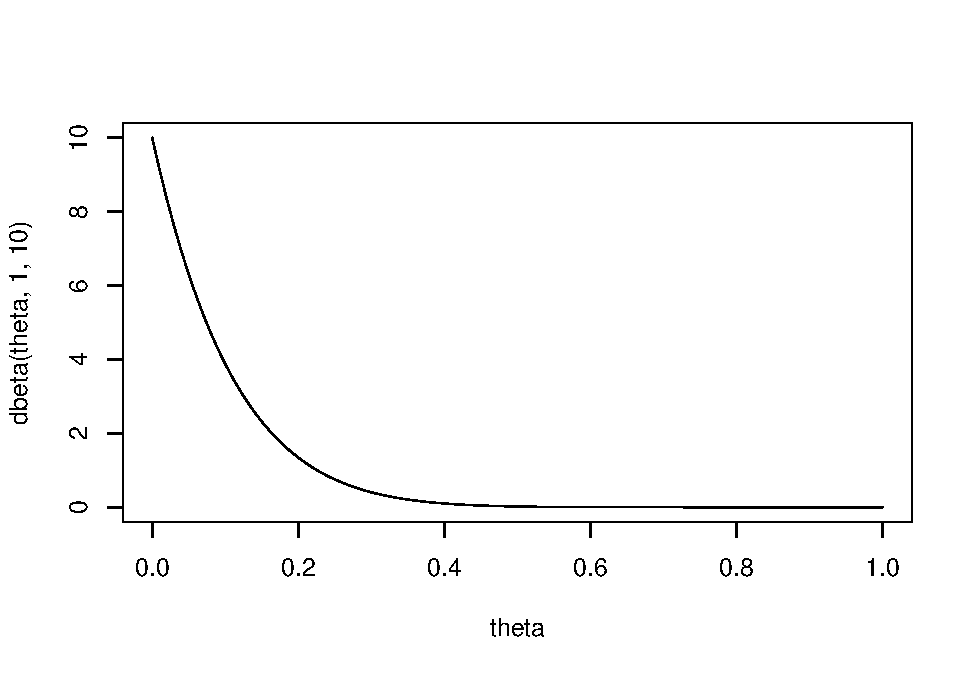
\includegraphics{_main_files/figure-latex/unnamed-chunk-6-1.pdf}

\begin{enumerate}
\def\labelenumi{(\alph{enumi})}
\setcounter{enumi}{1}
\tightlist
\item
  In the period of 1900-1992, there were 20,597 elections, out of which 6 were decided by less than 10 votes, and 49 were decided by less than 100 votes.\\
  we can estimate the probability of a tie to be less than 6/20,597 and bounded by 49/20,597. So for the Binomial trials the sum of the successes is 6, and n=20,597, so the posterior could be \(\theta | y \sim Beta(1+6, 10+20,597 -6)\) is the posterior for \(\theta\). This assumes that 10 votes is within the neighborhood of an election tie.\\
  The question asks to compute at least one election tie, from a total of 435 elections. This follows a Binomial(435, \(\hat{\theta})\). Where we use the posterior mean to estimate \(\theta\). The posterior mean using the Beta(7,20601) yields a mean of \(\hat{\theta}=\frac{7}{20608} = 3.4e-04\) as the posterior mean.
\end{enumerate}

Then the probability that at least 1 election is tied, from 435 total elections will follow a Binomial(435, \(\hat{\theta})\), where we can use the posterior distribution for \(\theta | y\) in the Binomial likelihood \(P(X\geq 1 | \hat{\theta})= 1-P(X\leq0 | \hat{\theta})\) which has a probability of 0.14 of at least 1 election tie.

\begin{Shaded}
\begin{Highlighting}[]
 \CommentTok{\# the posterior for theta is Beta(1+6,10+20597{-}6)}
 \FunctionTok{plot}\NormalTok{(theta,}\FunctionTok{dbeta}\NormalTok{(theta,}\DecValTok{7}\NormalTok{,}\DecValTok{10}\SpecialCharTok{+}\DecValTok{20597{-}6}\NormalTok{),}\AttributeTok{type=}\StringTok{\textquotesingle{}l\textquotesingle{}}\NormalTok{)}
\end{Highlighting}
\end{Shaded}

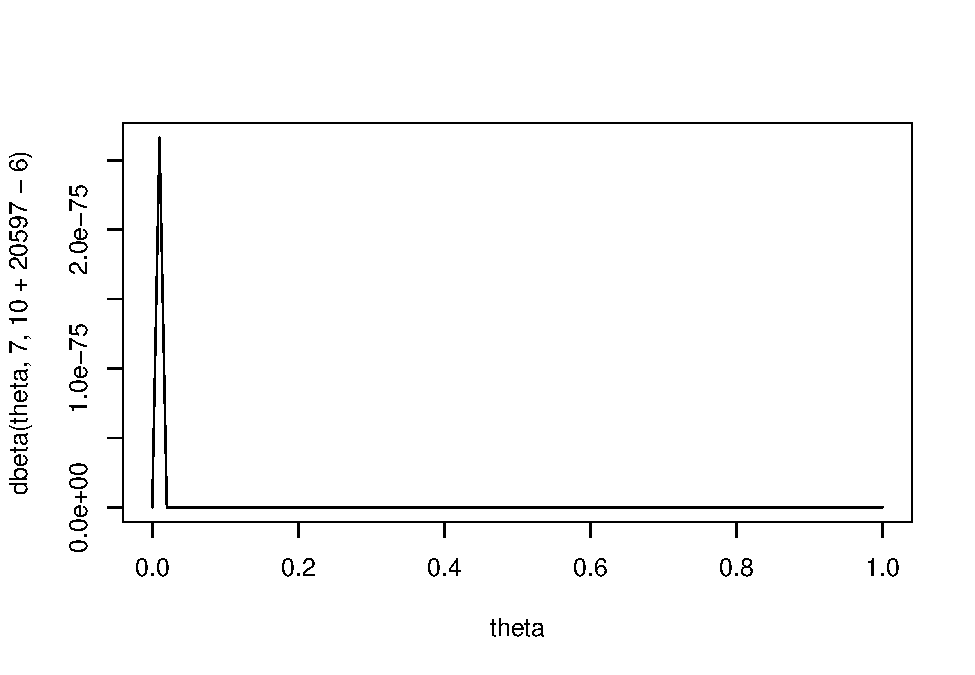
\includegraphics{_main_files/figure-latex/unnamed-chunk-7-1.pdf}

\begin{Shaded}
\begin{Highlighting}[]
 \DocumentationTok{\#\# posterior mean is 7/(20601)}
\DocumentationTok{\#\# then P(X\textgreater{}=1) = 1{-}P(X\textless{}=0 | p)}
  \DecValTok{1}\SpecialCharTok{{-}}\FunctionTok{pbinom}\NormalTok{(}\DecValTok{0}\NormalTok{,}\DecValTok{435}\NormalTok{,}\AttributeTok{prob=}\DecValTok{7}\SpecialCharTok{/}\DecValTok{20608}\NormalTok{)}
\end{Highlighting}
\end{Shaded}

\begin{verbatim}
## [1] 0.1373819
\end{verbatim}

\begin{enumerate}
\def\labelenumi{\arabic{enumi}.}
\setcounter{enumi}{8}
\item
  A clinic has three doctors. Patients come into the clinic at random, starting at 9 a.m. according to a Poisson process, with a time parameter, t, of 10 minutes; that is after opening the first patient appears follows an exponential distribution with average waiting time of 10 minutes. Then the next patient arrives with a waiting time of an expected 10 minutes as iid exponential distribution. After a patient arrives, the patient waits until a doctor is available, and the doctor visits a patitient uniformly between 5-20 minutes. The clinic stops admitting patients at 4 pm, and closes after the last patient is completed with the visit.

  \begin{enumerate}
  \def\labelenumii{(\alph{enumii})}
  \tightlist
  \item
    Simulate this process once. how many patients visited the office? how many had to wait for a doctor? what was the average wait? when did office close?
  \end{enumerate}
\end{enumerate}

\begin{Shaded}
\begin{Highlighting}[]
\DocumentationTok{\#\#\# waiting time for a new patient to arrive in the clinic}
\DocumentationTok{\#\#\#\#\#\#\#\#\#\#\#\#\#\#\#\#\#\#\#\#\#\#\#\#\#\#\#\#\#\#\#\#\#\#\#\#\#\#\#\#\#\#\#\#\#\#\#\#\#\#\#\#\#\#\#\#\#\#\#}
 \CommentTok{\# patientList is the data frame of all patients}
 \CommentTok{\# closeTime is the time to stop admitting (420 minutes)}
 \CommentTok{\# currentPatient Number }
 \CommentTok{\# current time is the running total of time}
\NormalTok{  newPatientArrival}\OtherTok{\textless{}{-}}\ControlFlowTok{function}\NormalTok{(patientList,}
                             \AttributeTok{closeTime=}\NormalTok{timeToClose,}
\NormalTok{                              waitTime,}
\NormalTok{                             visitTime,}
                             \AttributeTok{currentPatientNumber=}\DecValTok{0}\NormalTok{,}
\NormalTok{                             currentTime,}
                             \AttributeTok{assignedDoctor=}\StringTok{"none"}\NormalTok{,}
                             \AttributeTok{completionTime=}\DecValTok{0}\NormalTok{)\{}
    \CommentTok{\# waiting time for next patient}
\NormalTok{     patientTime}\OtherTok{\textless{}{-}}\FunctionTok{round}\NormalTok{(}\FunctionTok{rexp}\NormalTok{(}\DecValTok{1}\NormalTok{,}\AttributeTok{rate=}\DecValTok{1}\SpecialCharTok{/}\DecValTok{10}\NormalTok{),}\DecValTok{2}\NormalTok{)}
    \CommentTok{\# current time of existing patients}
\NormalTok{     current}\OtherTok{\textless{}{-}}\FunctionTok{max}\NormalTok{(patientList}\SpecialCharTok{$}\NormalTok{currentTime)}
   \DocumentationTok{\#\# the clinic stops admitting patients at 4pm}
   \ControlFlowTok{if}\NormalTok{( (current}\SpecialCharTok{+}\NormalTok{patientTime)}\SpecialCharTok{\textless{}=}\NormalTok{closeTime)\{}
     \DocumentationTok{\#\# in minutes}
\NormalTok{   newPatient}\OtherTok{\textless{}{-}}\FunctionTok{createPatientChart}\NormalTok{(currentPatientNumber,patientTime,waitTime,visitTime,currentTime,assignedDoctor,}\DecValTok{0}\NormalTok{)}
\NormalTok{    \}}\ControlFlowTok{else}\NormalTok{\{}
\NormalTok{    newPatient}\OtherTok{\textless{}{-}}\FunctionTok{createPatientChart}\NormalTok{(currentPatientNumber,patientTime,waitTime,visitTime,currentTime,}\StringTok{"closed\_notAdmitted"}\NormalTok{,}\DecValTok{0}\NormalTok{)}
\NormalTok{   \}}
   \FunctionTok{return}\NormalTok{(newPatient)}
\NormalTok{ \}}
\DocumentationTok{\#\#\#\#\#\#\#\#\#\#\#\#\#\#\#\#\#\#\#\# }
 
 
 
\NormalTok{ computeWaitTime}\OtherTok{\textless{}{-}}\ControlFlowTok{function}\NormalTok{(}\AttributeTok{doctors=}\ConstantTok{NULL}\NormalTok{,}
                           \AttributeTok{patientList=}\ConstantTok{NULL}\NormalTok{,}
                           \AttributeTok{patientID=}\DecValTok{1}\NormalTok{)\{}
   \DocumentationTok{\#\# need to compute visiting time (booked)}
   \DocumentationTok{\#\# next time available}
   \DocumentationTok{\#\# required input current time for a specific doctor/patient ?}
   \CommentTok{\# patient time (minutes)}
   
   \DocumentationTok{\#\# FIX ME: it is grabbing 2 patient IDs?}
\NormalTok{   currentTime}\OtherTok{\textless{}{-}}\NormalTok{patientList}\SpecialCharTok{$}\NormalTok{currentTime[}\FunctionTok{which}\NormalTok{(patientList}\SpecialCharTok{$}\NormalTok{patient}\SpecialCharTok{==}\NormalTok{patientID)]}
\NormalTok{   visitTime}\OtherTok{\textless{}{-}}\FunctionTok{runif}\NormalTok{(}\DecValTok{1}\NormalTok{,}\AttributeTok{min=}\DecValTok{5}\NormalTok{,}\AttributeTok{max=}\DecValTok{20}\NormalTok{) }\DocumentationTok{\#\# minutes}
 
   
   \ControlFlowTok{if}\NormalTok{(}\FunctionTok{any}\NormalTok{(doctors}\SpecialCharTok{$}\NormalTok{nextTimeAvail}\SpecialCharTok{\textless{}}\NormalTok{currentTime))\{}
\NormalTok{     waitTime}\OtherTok{=}\DecValTok{0}
\NormalTok{     assignedDr}\OtherTok{\textless{}{-}}\FunctionTok{sample}\NormalTok{(doctors}\SpecialCharTok{$}\NormalTok{dr[}\FunctionTok{which}\NormalTok{(doctors}\SpecialCharTok{$}\NormalTok{nextTimeAvail}\SpecialCharTok{\textless{}}\NormalTok{currentTime)],}\DecValTok{1}\NormalTok{)}
     \DocumentationTok{\#\#\# current time + visitTime}
\NormalTok{     nextAvailTime}\OtherTok{\textless{}{-}}\NormalTok{ visitTime}\SpecialCharTok{+}\NormalTok{currentTime}\SpecialCharTok{+}\NormalTok{waitTime}
     \DocumentationTok{\#\# completion time for patient exit (closing time).}
\NormalTok{   \}}\ControlFlowTok{else} \ControlFlowTok{if}\NormalTok{(}\FunctionTok{any}\NormalTok{(doctors}\SpecialCharTok{$}\NormalTok{nextTimeAvail}\SpecialCharTok{\textless{}}\NormalTok{currentTime)}\SpecialCharTok{==}\ConstantTok{FALSE}\NormalTok{)\{}
     \CommentTok{\# all doctors are booked, no available doctors.}
     \CommentTok{\# wait time is the difference between next available time (assuming all times are greater than patient time)}
\NormalTok{     waitTime}\OtherTok{\textless{}{-}}\FunctionTok{min}\NormalTok{(doctors}\SpecialCharTok{$}\NormalTok{nextTimeAvail}\SpecialCharTok{{-}}\NormalTok{currentTime)}
\NormalTok{     assignedDr}\OtherTok{\textless{}{-}}\NormalTok{doctors}\SpecialCharTok{$}\NormalTok{dr[}\FunctionTok{which}\NormalTok{( (doctors}\SpecialCharTok{$}\NormalTok{nextTimeAvail}\SpecialCharTok{{-}}\NormalTok{currentTime)}\SpecialCharTok{==}\FunctionTok{min}\NormalTok{(doctors}\SpecialCharTok{$}\NormalTok{nextTimeAvail}\SpecialCharTok{{-}}\NormalTok{currentTime))]}
       \ControlFlowTok{if}\NormalTok{(}\FunctionTok{length}\NormalTok{(assignedDr)}\SpecialCharTok{\textgreater{}}\DecValTok{1}\NormalTok{)\{}
\NormalTok{         assignedDr}\OtherTok{\textless{}{-}}\NormalTok{assignedDr[}\DecValTok{1}\NormalTok{]}
\NormalTok{       \}}
\NormalTok{     nextAvailTime}\OtherTok{\textless{}{-}}\NormalTok{ visitTime}\SpecialCharTok{+}\NormalTok{currentTime}\SpecialCharTok{+}\NormalTok{waitTime  }\DocumentationTok{\#\# completion time for patient to exit}
\NormalTok{    \}}\DocumentationTok{\#\# if all doctors unavail}
    \CommentTok{\#print(assignedDr)}
    \CommentTok{\#print(currentTime)}
    \DocumentationTok{\#\#  update doctor list}
\NormalTok{     doctors[}\FunctionTok{which}\NormalTok{(doctors}\SpecialCharTok{$}\NormalTok{dr}\SpecialCharTok{==}\NormalTok{assignedDr),}\StringTok{\textquotesingle{}visitingPatient\textquotesingle{}}\NormalTok{]}\OtherTok{\textless{}{-}}\NormalTok{patientID}
\NormalTok{     doctors[}\FunctionTok{which}\NormalTok{(doctors}\SpecialCharTok{$}\NormalTok{dr}\SpecialCharTok{==}\NormalTok{assignedDr),}\StringTok{\textquotesingle{}nextTimeAvail\textquotesingle{}}\NormalTok{]}\OtherTok{\textless{}{-}}\NormalTok{nextAvailTime}
\NormalTok{     doctors[}\FunctionTok{which}\NormalTok{(doctors}\SpecialCharTok{$}\NormalTok{dr}\SpecialCharTok{==}\NormalTok{assignedDr),}\StringTok{\textquotesingle{}currentTime\textquotesingle{}}\NormalTok{]}\OtherTok{\textless{}{-}}\NormalTok{currentTime }\DocumentationTok{\#\# patient time}
\NormalTok{     doctors[}\FunctionTok{which}\NormalTok{(doctors}\SpecialCharTok{$}\NormalTok{dr}\SpecialCharTok{==}\NormalTok{assignedDr),}\StringTok{\textquotesingle{}visitTimeLength\textquotesingle{}}\NormalTok{]}\OtherTok{\textless{}{-}}\NormalTok{visitTime}
     \CommentTok{\# flag avail to no.}
\NormalTok{     doctors[}\FunctionTok{which}\NormalTok{(doctors}\SpecialCharTok{$}\NormalTok{dr}\SpecialCharTok{==}\NormalTok{assignedDr),}\StringTok{\textquotesingle{}avail\textquotesingle{}}\NormalTok{]}\OtherTok{\textless{}{-}}\StringTok{\textquotesingle{}no\textquotesingle{}}
     \DocumentationTok{\#\# update patient list}
\NormalTok{     patientList[}\FunctionTok{which}\NormalTok{(patientList}\SpecialCharTok{$}\NormalTok{patient}\SpecialCharTok{==}\NormalTok{patientID),}\StringTok{\textquotesingle{}doctorWaitTime\textquotesingle{}}\NormalTok{]}\OtherTok{\textless{}{-}}\NormalTok{waitTime}
\NormalTok{     patientList[}\FunctionTok{which}\NormalTok{(patientList}\SpecialCharTok{$}\NormalTok{patient}\SpecialCharTok{==}\NormalTok{patientID),}\StringTok{\textquotesingle{}doctorVisitTime\textquotesingle{}}\NormalTok{]}\OtherTok{\textless{}{-}}\NormalTok{visitTime}
\NormalTok{     patientList[}\FunctionTok{which}\NormalTok{(patientList}\SpecialCharTok{$}\NormalTok{patient}\SpecialCharTok{==}\NormalTok{patientID),}\StringTok{\textquotesingle{}assignedDoctor\textquotesingle{}}\NormalTok{]}\OtherTok{\textless{}{-}}\NormalTok{assignedDr}
\NormalTok{     patientList[}\FunctionTok{which}\NormalTok{(patientList}\SpecialCharTok{$}\NormalTok{patient}\SpecialCharTok{==}\NormalTok{patientID),}\StringTok{\textquotesingle{}completionTime\textquotesingle{}}\NormalTok{]}\OtherTok{\textless{}{-}}\NormalTok{nextAvailTime}
   \FunctionTok{return}\NormalTok{(}\FunctionTok{list}\NormalTok{(}\AttributeTok{patient=}\NormalTok{patientList,}\AttributeTok{doctor=}\NormalTok{doctors))}
\NormalTok{ \}}
 
 
 \DocumentationTok{\#\# creates a patient object}
\NormalTok{ createPatientChart}\OtherTok{\textless{}{-}}\ControlFlowTok{function}\NormalTok{(currentPatientNumber,arrivalTime,waitTime,visitTime,currentTime,assignedDoctor,completionTime)\{}
\NormalTok{   patientID}\OtherTok{\textless{}{-}}\FunctionTok{data.frame}\NormalTok{(}\AttributeTok{patient=}\NormalTok{currentPatientNumber}\SpecialCharTok{+}\DecValTok{1}\NormalTok{,}
                         \AttributeTok{arrivalTime=}\NormalTok{arrivalTime,}
                         \AttributeTok{doctorWaitTime=}\NormalTok{waitTime,}
                         \AttributeTok{doctorVisitTime=}\NormalTok{visitTime,}
                         \AttributeTok{currentTime=}\NormalTok{currentTime,}
                         \AttributeTok{assignedDoctor=}\NormalTok{assignedDoctor,}
                         \AttributeTok{completionTime=}\DecValTok{0}\NormalTok{)}
   \FunctionTok{return}\NormalTok{(patientID)}
\NormalTok{ \}}
 
\NormalTok{ updatePatientList}\OtherTok{\textless{}{-}}\ControlFlowTok{function}\NormalTok{(patientList,patientID)\{}
\NormalTok{   patientList}\OtherTok{\textless{}{-}}\FunctionTok{rbind}\NormalTok{(patientList,patientID)}
   \FunctionTok{return}\NormalTok{(patientList)}
\NormalTok{ \}}
 
\NormalTok{updateTime}\OtherTok{\textless{}{-}}\ControlFlowTok{function}\NormalTok{(currentTime,}\AttributeTok{newTime=}\ConstantTok{NULL}\NormalTok{,p1)\{}
\NormalTok{  p1}\SpecialCharTok{$}\NormalTok{currentTime}\OtherTok{\textless{}{-}}\NormalTok{currentTime}\SpecialCharTok{+}\NormalTok{newTime}
  \FunctionTok{return}\NormalTok{(p1)}
\NormalTok{\}}
\NormalTok{ totalPatients}\OtherTok{\textless{}{-}}\DecValTok{0}
\DocumentationTok{\#\# this is the simulation}
 \DocumentationTok{\#\# first task : loop through the time update for patients}
 \DocumentationTok{\#\# second task : include the doctor assignment query.}
\NormalTok{simulateProcess}\OtherTok{\textless{}{-}}\ControlFlowTok{function}\NormalTok{(}\AttributeTok{doctors=}\ConstantTok{NULL}\NormalTok{,}
                          \AttributeTok{totalWait=}\ConstantTok{NULL}\NormalTok{,}
                          \AttributeTok{totalPatients=}\DecValTok{0}\NormalTok{,}
                          \AttributeTok{timeToClose=}\DecValTok{420}\NormalTok{,}
                          \AttributeTok{currentTime=}\ConstantTok{NULL}\NormalTok{)\{}
  \DocumentationTok{\#\# initiate Patient List}
\NormalTok{ patientList}\OtherTok{\textless{}{-}}\FunctionTok{data.frame}\NormalTok{(}\AttributeTok{patient=}\DecValTok{0}\NormalTok{,}
                         \AttributeTok{arrivalTime=}\DecValTok{0}\NormalTok{,}
                         \AttributeTok{doctorWaitTime=}\DecValTok{0}\NormalTok{,}
                         \AttributeTok{doctorVisitTime=}\DecValTok{0}\NormalTok{,}
                         \AttributeTok{currentTime=}\DecValTok{0}\NormalTok{,}
                         \AttributeTok{assignedDoctor=}\StringTok{\textquotesingle{}none\textquotesingle{}}\NormalTok{,}
                         \AttributeTok{completionTime=}\DecValTok{0}\NormalTok{)}
 \DocumentationTok{\#\# not sure what to put here.}
\NormalTok{ currentTime}\OtherTok{\textless{}{-}}\NormalTok{patientList}\SpecialCharTok{$}\NormalTok{currentTime[}\FunctionTok{which}\NormalTok{(patientList}\SpecialCharTok{$}\NormalTok{patient}\SpecialCharTok{==}\FunctionTok{max}\NormalTok{(patientList}\SpecialCharTok{$}\NormalTok{patient))] }\DocumentationTok{\#\# current time is the max current time from patient chart.}
\NormalTok{ currentPatientNumber}\OtherTok{\textless{}{-}}\DecValTok{0}
 
 \DocumentationTok{\#\# timeToClose (minutes) is stopping to admit patients}
  \ControlFlowTok{while}\NormalTok{(currentTime}\SpecialCharTok{\textless{}}\NormalTok{timeToClose)\{}
    \DocumentationTok{\#\# patient enters after the (i{-}1) patient enters.}
\NormalTok{    p1}\OtherTok{\textless{}{-}}\FunctionTok{newPatientArrival}\NormalTok{(patientList,}
                             \AttributeTok{closeTime=}\NormalTok{timeToClose,}
                          \AttributeTok{waitTime=}\DecValTok{0}\NormalTok{,}
                          \AttributeTok{visitTime=}\DecValTok{0}\NormalTok{,}
                             \AttributeTok{currentPatientNumber=}\NormalTok{currentPatientNumber,}
\NormalTok{                             currentTime)}
    \DocumentationTok{\#\# update time}
\NormalTok{    p1}\OtherTok{\textless{}{-}}\FunctionTok{updateTime}\NormalTok{(p1}\SpecialCharTok{$}\NormalTok{currentTime,}\AttributeTok{newTime=}\NormalTok{p1}\SpecialCharTok{$}\NormalTok{arrivalTime,p1)}
    
    \CommentTok{\# given a patient time, switch the availability of any doctor}
    \CommentTok{\# if a doctors next available time is less than the current time, switch him to available}
    \DocumentationTok{\#\# FIX ME: need to ensure this flag is correct.}
    \ControlFlowTok{if}\NormalTok{(}\FunctionTok{any}\NormalTok{(doctors}\SpecialCharTok{$}\NormalTok{nextTimeAvail}\SpecialCharTok{\textless{}}\NormalTok{p1}\SpecialCharTok{$}\NormalTok{currentTime))\{}
\NormalTok{      doctors}\SpecialCharTok{$}\NormalTok{avail[}\FunctionTok{which}\NormalTok{(doctors}\SpecialCharTok{$}\NormalTok{nextTimeAvail}\SpecialCharTok{\textless{}}\NormalTok{p1}\SpecialCharTok{$}\NormalTok{currentTime)]}\OtherTok{\textless{}{-}}\StringTok{\textquotesingle{}yes\textquotesingle{}}
\NormalTok{    \}}
    
    \DocumentationTok{\#\# create a patient list}
    \ControlFlowTok{if}\NormalTok{(currentPatientNumber}\SpecialCharTok{==}\DecValTok{0}\NormalTok{)\{}
\NormalTok{      patientList}\OtherTok{\textless{}{-}}\NormalTok{p1}
     \CommentTok{\# update patient number  }
\NormalTok{      currentPatientNumber}\OtherTok{\textless{}{-}}\NormalTok{currentPatientNumber}\SpecialCharTok{+}\DecValTok{1}
\NormalTok{    \}}\ControlFlowTok{else}\NormalTok{\{}
\NormalTok{      patientList}\OtherTok{\textless{}{-}}\FunctionTok{rbind}\NormalTok{(patientList,p1)}
     \CommentTok{\# update patient number  }
\NormalTok{      currentPatientNumber}\OtherTok{\textless{}{-}}\NormalTok{currentPatientNumber}\SpecialCharTok{+}\DecValTok{1}
\NormalTok{    \}}
    
    \DocumentationTok{\#\# task 2 assign a doctor}
     \DocumentationTok{\#\#\# check for doctor availability}
     \DocumentationTok{\#\# compute wait time, and/or compute the next available time}
     \DocumentationTok{\#\# returns a list object.}
\NormalTok{    clinicList}\OtherTok{\textless{}{-}}\FunctionTok{computeWaitTime}\NormalTok{(doctors,patientList,}\AttributeTok{patientID=}\NormalTok{patientList}\SpecialCharTok{$}\NormalTok{patient[currentPatientNumber])}
  
\NormalTok{    doctors}\OtherTok{\textless{}{-}}\NormalTok{clinicList[[}\StringTok{"doctor"}\NormalTok{]]}
\NormalTok{   patientList}\OtherTok{\textless{}{-}}\NormalTok{clinicList[[}\StringTok{"patient"}\NormalTok{]]}
   \DocumentationTok{\#\# update flags}
     \CommentTok{\# update currentTime}
    \DocumentationTok{\#\# current time is cumulative sum of the arrival times.}
\NormalTok{   currentTime}\OtherTok{\textless{}{-}}\NormalTok{patientList}\SpecialCharTok{$}\NormalTok{currentTime[}\FunctionTok{which}\NormalTok{(patientList}\SpecialCharTok{$}\NormalTok{patient}\SpecialCharTok{==}\FunctionTok{max}\NormalTok{(patientList}\SpecialCharTok{$}\NormalTok{patient))] }\DocumentationTok{\#\# current time is the max current time from patient chart.}
   
   \DocumentationTok{\#\# fix me:}
   \DocumentationTok{\#\# reset doctor availability based on current patient time.}
\NormalTok{   upID}\OtherTok{\textless{}{-}}\FunctionTok{which}\NormalTok{(doctors}\SpecialCharTok{$}\NormalTok{nextTimeAvail}\SpecialCharTok{\textless{}}\NormalTok{currentTime)}
\NormalTok{   doctors}\SpecialCharTok{$}\NormalTok{nextTimeAvail[upID]}\OtherTok{\textless{}{-}}\NormalTok{currentTime}
\NormalTok{   doctors}\SpecialCharTok{$}\NormalTok{currentTime[upID]}\OtherTok{\textless{}{-}}\NormalTok{currentTime }
\NormalTok{   doctors}\SpecialCharTok{$}\NormalTok{visitTimeLength[upID]}\OtherTok{\textless{}{-}}\DecValTok{0} 
\NormalTok{  \}}\DocumentationTok{\#\# while loop}
  \FunctionTok{return}\NormalTok{(}\FunctionTok{list}\NormalTok{(}\AttributeTok{patient=}\NormalTok{patientList,}\AttributeTok{doctors=}\NormalTok{doctors))}
\NormalTok{\}}
\end{Highlighting}
\end{Shaded}

\begin{Shaded}
\begin{Highlighting}[]
\NormalTok{ doctors}\OtherTok{\textless{}{-}}\FunctionTok{data.frame}\NormalTok{(}\AttributeTok{dr=}\FunctionTok{c}\NormalTok{(}\StringTok{\textquotesingle{}a\textquotesingle{}}\NormalTok{,}\StringTok{\textquotesingle{}b\textquotesingle{}}\NormalTok{,}\StringTok{\textquotesingle{}c\textquotesingle{}}\NormalTok{),}
                     \AttributeTok{visitingPatient=}\FunctionTok{c}\NormalTok{(}\DecValTok{0}\NormalTok{,}\DecValTok{0}\NormalTok{,}\DecValTok{0}\NormalTok{), }\DocumentationTok{\#\# who is doctor seeing (patient ID)}
                     \AttributeTok{visitTimeLength=}\FunctionTok{c}\NormalTok{(}\DecValTok{0}\NormalTok{,}\DecValTok{0}\NormalTok{,}\DecValTok{0}\NormalTok{), }\CommentTok{\# length of doctor visit U(5,20)}
                     \AttributeTok{currentTime=}\FunctionTok{c}\NormalTok{(}\DecValTok{0}\NormalTok{,}\DecValTok{0}\NormalTok{,}\DecValTok{0}\NormalTok{),    }\DocumentationTok{\#\# current Time}
                     \AttributeTok{nextTimeAvail=}\FunctionTok{c}\NormalTok{(}\DecValTok{0}\NormalTok{,}\DecValTok{0}\NormalTok{,}\DecValTok{0}\NormalTok{),  }\DocumentationTok{\#\# current time + visitTimeLength = next avail time.}
                     \AttributeTok{avail=}\FunctionTok{c}\NormalTok{(}\StringTok{"yes"}\NormalTok{,}\StringTok{"yes"}\NormalTok{,}\StringTok{"yes"}\NormalTok{))}
\DocumentationTok{\#\# initiate times}
\NormalTok{ totalWait}\OtherTok{\textless{}{-}}\DecValTok{0}
\NormalTok{ currentPatientNumber}\OtherTok{\textless{}{-}}\DecValTok{0}
 \DocumentationTok{\#\# clinic opens at 9am {-}4pm that is 7 hours (420 min.)}
\NormalTok{ timeToClose}\OtherTok{\textless{}{-}}\DecValTok{7}\SpecialCharTok{*}\DecValTok{60} \DocumentationTok{\#\# stops admiting patienets in 420 minutes}
 \DocumentationTok{\#\# current time is 0}
 \DocumentationTok{\#\# this will be the running total of minutes.}
\NormalTok{ currentTime}\OtherTok{\textless{}{-}}\DecValTok{0}
 
 
 
\NormalTok{res}\OtherTok{\textless{}{-}}\FunctionTok{simulateProcess}\NormalTok{(doctors,}
\NormalTok{                          totalWait,}
\NormalTok{                          totalPatients,}
\NormalTok{                          timeToClose,}
\NormalTok{                          currentTime)}

\NormalTok{pl}\OtherTok{\textless{}{-}}\NormalTok{res}\SpecialCharTok{$}\NormalTok{patient[}\FunctionTok{which}\NormalTok{(res}\SpecialCharTok{$}\NormalTok{patient}\SpecialCharTok{$}\NormalTok{currentTime}\SpecialCharTok{\textless{}=}\DecValTok{420}\NormalTok{),]}

 \FunctionTok{hist}\NormalTok{(pl}\SpecialCharTok{$}\NormalTok{doctorVisitTime)}
 \FunctionTok{abline}\NormalTok{(}\AttributeTok{v=}\NormalTok{(}\DecValTok{20}\SpecialCharTok{+}\DecValTok{5}\NormalTok{)}\SpecialCharTok{/}\DecValTok{2}\NormalTok{) }\DocumentationTok{\#\# should be \textasciitilde{}12}
\end{Highlighting}
\end{Shaded}

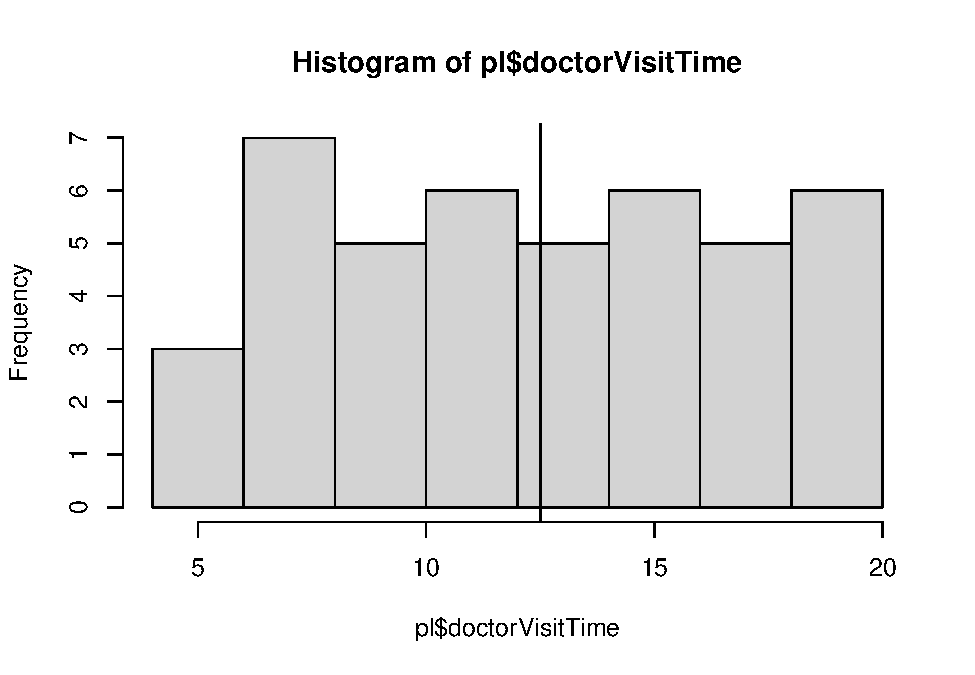
\includegraphics{_main_files/figure-latex/unnamed-chunk-9-1.pdf}

\begin{Shaded}
\begin{Highlighting}[]
 \FunctionTok{hist}\NormalTok{(pl}\SpecialCharTok{$}\NormalTok{arrivalTime) }\DocumentationTok{\#\# should be close to 10  exp(1/10) has mean 10}
\end{Highlighting}
\end{Shaded}

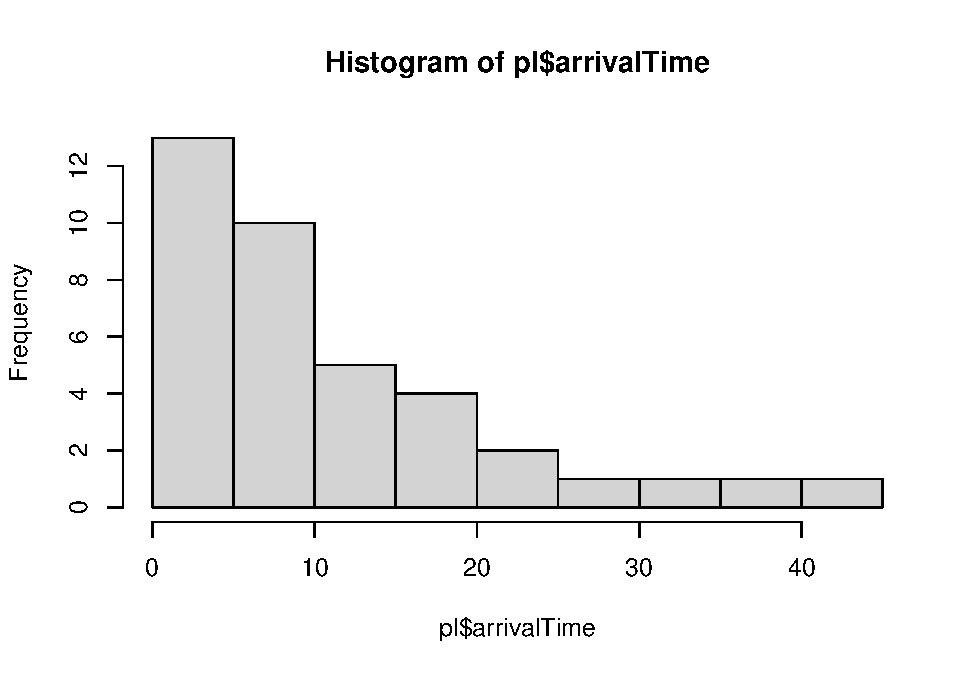
\includegraphics{_main_files/figure-latex/unnamed-chunk-9-2.pdf}

\begin{Shaded}
\begin{Highlighting}[]
  \FunctionTok{hist}\NormalTok{(pl}\SpecialCharTok{$}\NormalTok{doctorWaitTime[}\FunctionTok{which}\NormalTok{(pl}\SpecialCharTok{$}\NormalTok{doctorWaitTime}\SpecialCharTok{!=}\DecValTok{0}\NormalTok{)]) }\DocumentationTok{\#\# about 2.41}
\end{Highlighting}
\end{Shaded}

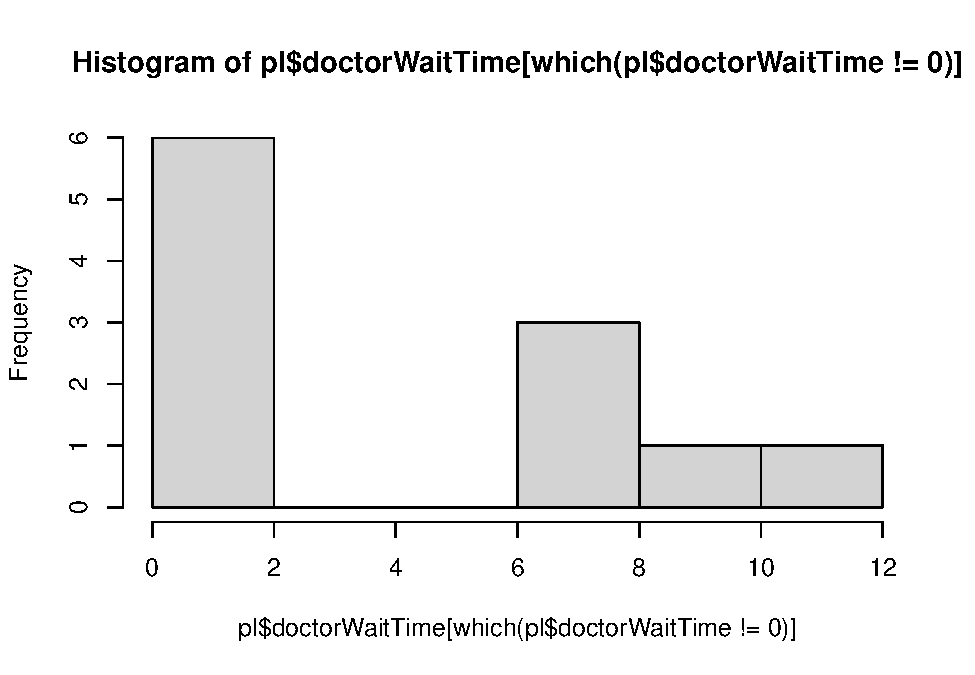
\includegraphics{_main_files/figure-latex/unnamed-chunk-9-3.pdf}

\begin{Shaded}
\begin{Highlighting}[]
  \FunctionTok{print}\NormalTok{(}\FunctionTok{max}\NormalTok{(pl}\SpecialCharTok{$}\NormalTok{completionTime)}\SpecialCharTok{{-}}\DecValTok{420}\NormalTok{) }\DocumentationTok{\#\# closing time}
\end{Highlighting}
\end{Shaded}

\begin{verbatim}
## [1] -2.781885
\end{verbatim}

\begin{Shaded}
\begin{Highlighting}[]
  \FunctionTok{print}\NormalTok{(}\FunctionTok{max}\NormalTok{(pl}\SpecialCharTok{$}\NormalTok{patient)) }\DocumentationTok{\#\# total patient  should be 42}
\end{Highlighting}
\end{Shaded}

\begin{verbatim}
## [1] 45
\end{verbatim}

\begin{Shaded}
\begin{Highlighting}[]
\DocumentationTok{\#\# (20{-}5)/6 + 10 this is about 12.5 minutes of arrival + visit time. which is approximately close to 10 }
\DocumentationTok{\#\# the arrival time is about 10 minutes.  }

\DocumentationTok{\#\# we should expect 42 patients}
 \CommentTok{\#420/10}
  
  \DocumentationTok{\#\# sanity check}
  \CommentTok{\#all(pl$currentTime+pl$doctorWaitTime+pl$doctorVisitTime{-}pl$completionTime==0)}
\end{Highlighting}
\end{Shaded}

\hypertarget{simulation-100-times}{%
\section*{Simulation 100 times}\label{simulation-100-times}}
\addcontentsline{toc}{section}{Simulation 100 times}

total number of patients was approximately 42, which we expect since the total 420/10. The total number waiting with 3 doctors is 6.61 for 1 day. the average waiting time was about 4-5 minutes. For 1 day, the average closing time was 5.32 minutes after 4 pm

\begin{Shaded}
\begin{Highlighting}[]
\NormalTok{ totalPat}\OtherTok{\textless{}{-}}\ConstantTok{NULL}
\NormalTok{ totalWaiting}\OtherTok{\textless{}{-}}\ConstantTok{NULL}
\NormalTok{ avgWaiting}\OtherTok{\textless{}{-}}\ConstantTok{NULL}
\NormalTok{ closing}\OtherTok{\textless{}{-}}\ConstantTok{NULL}
\NormalTok{ patientList}\OtherTok{\textless{}{-}}\ConstantTok{NULL}
\NormalTok{ p1}\OtherTok{\textless{}{-}}\ConstantTok{NULL}
 
\ControlFlowTok{for}\NormalTok{(i }\ControlFlowTok{in} \DecValTok{1}\SpecialCharTok{:}\DecValTok{100}\NormalTok{)\{}
  
\NormalTok{ doctors}\OtherTok{\textless{}{-}}\FunctionTok{data.frame}\NormalTok{(}\AttributeTok{dr=}\FunctionTok{c}\NormalTok{(}\StringTok{\textquotesingle{}a\textquotesingle{}}\NormalTok{,}\StringTok{\textquotesingle{}b\textquotesingle{}}\NormalTok{,}\StringTok{\textquotesingle{}c\textquotesingle{}}\NormalTok{),}
                     \AttributeTok{visitingPatient=}\FunctionTok{c}\NormalTok{(}\DecValTok{0}\NormalTok{,}\DecValTok{0}\NormalTok{,}\DecValTok{0}\NormalTok{), }\DocumentationTok{\#\# who is doctor seeing (patient ID)}
                     \AttributeTok{visitTimeLength=}\FunctionTok{c}\NormalTok{(}\DecValTok{0}\NormalTok{,}\DecValTok{0}\NormalTok{,}\DecValTok{0}\NormalTok{), }\CommentTok{\# length of doctor visit U(5,20)}
                     \AttributeTok{currentTime=}\FunctionTok{c}\NormalTok{(}\DecValTok{0}\NormalTok{,}\DecValTok{0}\NormalTok{,}\DecValTok{0}\NormalTok{),    }\DocumentationTok{\#\# current Time}
                     \AttributeTok{nextTimeAvail=}\FunctionTok{c}\NormalTok{(}\DecValTok{0}\NormalTok{,}\DecValTok{0}\NormalTok{,}\DecValTok{0}\NormalTok{),  }\DocumentationTok{\#\# current time + visitTimeLength = next avail time.}
                     \AttributeTok{avail=}\FunctionTok{c}\NormalTok{(}\StringTok{"yes"}\NormalTok{,}\StringTok{"yes"}\NormalTok{,}\StringTok{"yes"}\NormalTok{))}
\DocumentationTok{\#\# initiate times}
\NormalTok{ totalWait}\OtherTok{\textless{}{-}}\DecValTok{0}
\NormalTok{ totalPatients}\OtherTok{\textless{}{-}}\DecValTok{0}
\NormalTok{ currentPatientNumber}\OtherTok{\textless{}{-}}\DecValTok{0}
 \DocumentationTok{\#\# clinic opens at 9am {-}4pm that is 7 hours (420 min.)}
\NormalTok{ timeToClose}\OtherTok{\textless{}{-}}\DecValTok{7}\SpecialCharTok{*}\DecValTok{60} \DocumentationTok{\#\# stops admiting patienets in 420 minutes}
 \DocumentationTok{\#\# current time is 0}
 \DocumentationTok{\#\# this will be the running total of minutes.}
\NormalTok{ currentTime}\OtherTok{\textless{}{-}}\DecValTok{0}
 
 
\NormalTok{res}\OtherTok{\textless{}{-}}\FunctionTok{simulateProcess}\NormalTok{(doctors,}
\NormalTok{                          totalWait,}
\NormalTok{                          totalPatients,}
\NormalTok{                          timeToClose,}
\NormalTok{                          currentTime)}

\NormalTok{pl}\OtherTok{\textless{}{-}}\NormalTok{res}\SpecialCharTok{$}\NormalTok{patient[}\FunctionTok{which}\NormalTok{(res}\SpecialCharTok{$}\NormalTok{patient}\SpecialCharTok{$}\NormalTok{currentTime}\SpecialCharTok{\textless{}=}\DecValTok{420}\NormalTok{),]}


\NormalTok{ totalPat}\OtherTok{\textless{}{-}}\FunctionTok{c}\NormalTok{(totalPat,}\FunctionTok{max}\NormalTok{(pl}\SpecialCharTok{$}\NormalTok{patient))}
\NormalTok{  totalWaiting}\OtherTok{\textless{}{-}}\FunctionTok{c}\NormalTok{(totalWaiting,}\FunctionTok{nrow}\NormalTok{(pl[}\FunctionTok{which}\NormalTok{(pl}\SpecialCharTok{$}\NormalTok{doctorWaitTime}\SpecialCharTok{!=}\DecValTok{0}\NormalTok{),]))}
\NormalTok{ avgWaiting}\OtherTok{\textless{}{-}}\FunctionTok{c}\NormalTok{(avgWaiting,}\FunctionTok{mean}\NormalTok{(pl[}\FunctionTok{which}\NormalTok{(pl}\SpecialCharTok{$}\NormalTok{doctorWaitTime}\SpecialCharTok{!=}\DecValTok{0}\NormalTok{),}\StringTok{"doctorWaitTime"}\NormalTok{]))}
\NormalTok{ closing}\OtherTok{\textless{}{-}}\FunctionTok{c}\NormalTok{(closing,}\FunctionTok{max}\NormalTok{(pl}\SpecialCharTok{$}\NormalTok{completionTime))}
 
\NormalTok{\}}
 
 \FunctionTok{hist}\NormalTok{(totalPat,}\AttributeTok{main=}\StringTok{"total patients"}\NormalTok{)}
 \FunctionTok{abline}\NormalTok{(}\AttributeTok{v=}\DecValTok{420}\SpecialCharTok{/}\DecValTok{10}\NormalTok{,}\AttributeTok{col=}\StringTok{\textquotesingle{}red\textquotesingle{}}\NormalTok{)}
\end{Highlighting}
\end{Shaded}

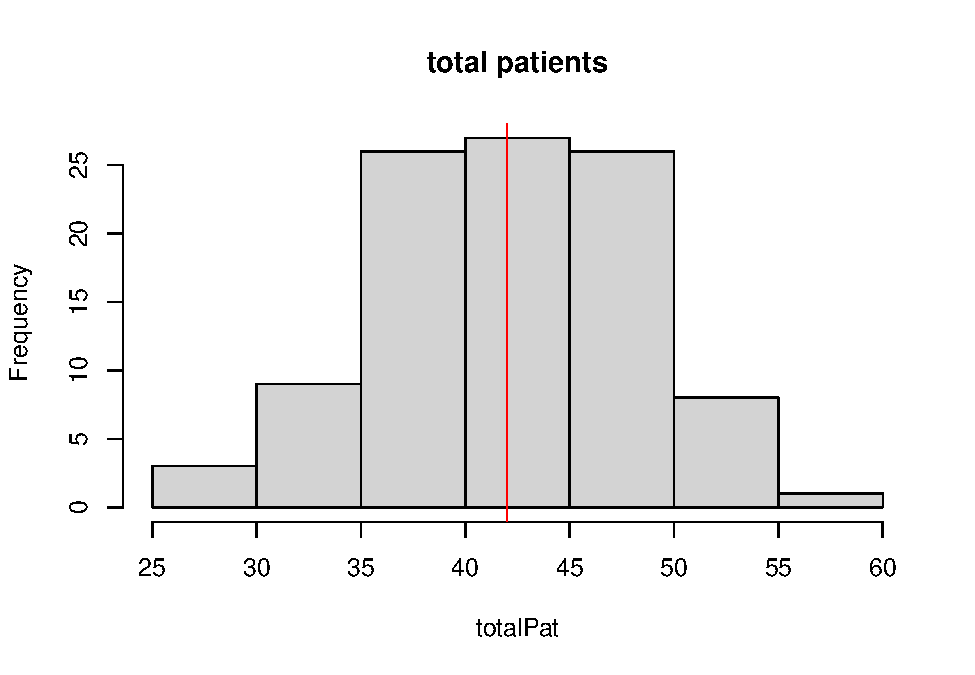
\includegraphics{_main_files/figure-latex/unnamed-chunk-10-1.pdf}

\begin{Shaded}
\begin{Highlighting}[]
 \FunctionTok{hist}\NormalTok{(totalWaiting,}\AttributeTok{main=}\StringTok{"total number waiting"}\NormalTok{)}
\end{Highlighting}
\end{Shaded}

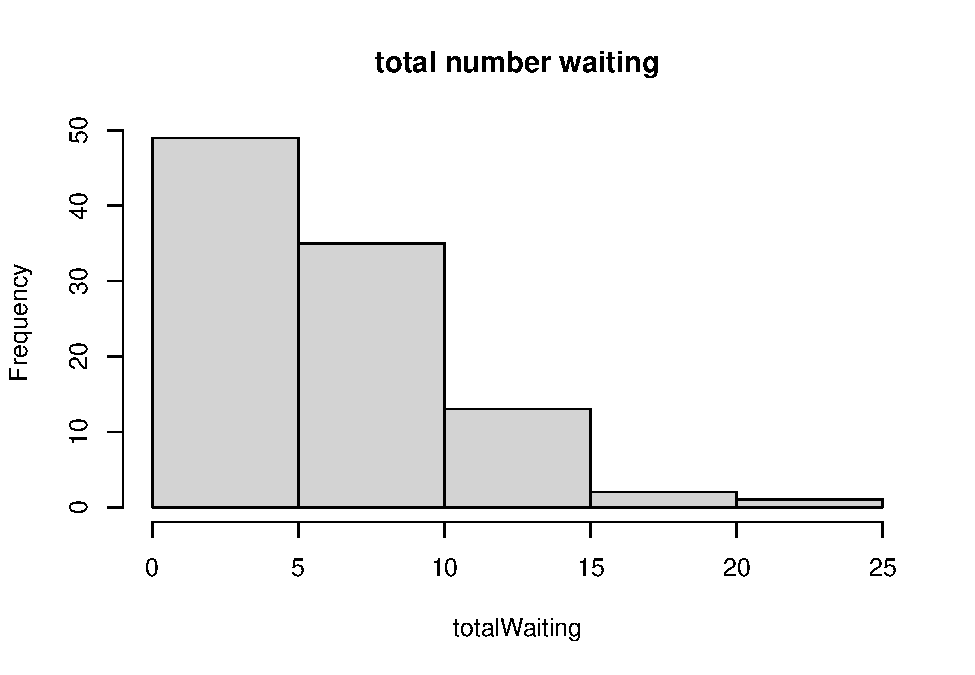
\includegraphics{_main_files/figure-latex/unnamed-chunk-10-2.pdf}

\begin{Shaded}
\begin{Highlighting}[]
 \FunctionTok{hist}\NormalTok{(avgWaiting,}\AttributeTok{main=}\StringTok{"avg. waiting (min)"}\NormalTok{)}
\end{Highlighting}
\end{Shaded}

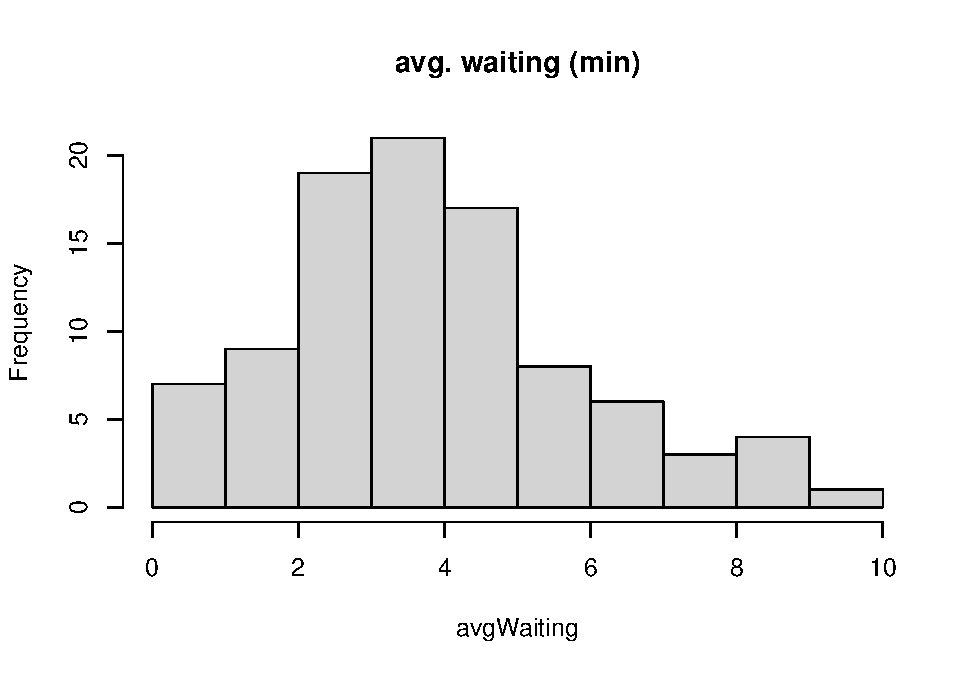
\includegraphics{_main_files/figure-latex/unnamed-chunk-10-3.pdf}

\begin{Shaded}
\begin{Highlighting}[]
 \FunctionTok{hist}\NormalTok{(closing}\DecValTok{{-}420}\NormalTok{,}\AttributeTok{main=}\StringTok{"closing time"}\NormalTok{)}
\end{Highlighting}
\end{Shaded}

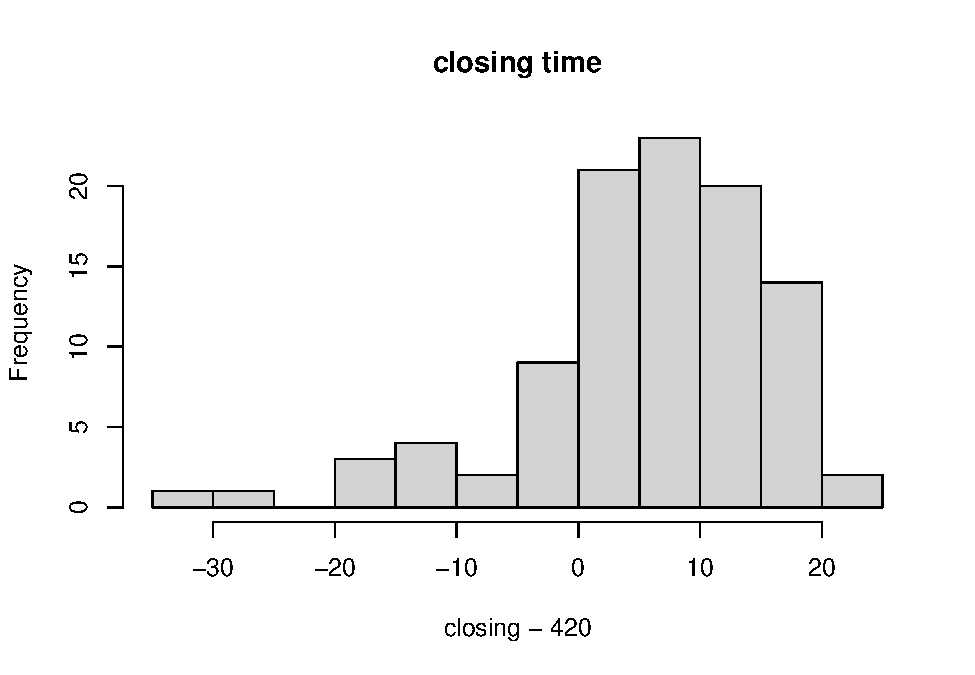
\includegraphics{_main_files/figure-latex/unnamed-chunk-10-4.pdf}

\hypertarget{cross}{%
\chapter{Single parameter models}\label{cross}}

\hypertarget{estimating-a-probability-from-binomial-data}{%
\section{Estimating a probability from binomial data}\label{estimating-a-probability-from-binomial-data}}

\begin{equation}
p(y  | \theta) = {n \choose y}\theta^y(1-\theta)^{n-y}
\label{eq:binomialProb}
\end{equation}

To perform Bayesian inference we assume \(\theta \sim U(0,1)\) where the posterior is

\begin{equation}
p(\theta | y) \propto \theta^y(1-\theta)^{n-y}
\label{eq:binomialPosterior}
\end{equation}

which is the form of a \texttt{beta} distribution \(\theta | y \sim Beta(y+1, n-y+1)\)

\hypertarget{posterior-as-a-compromise-between-data-and-prior-information}{%
\section{Posterior as a compromise between data and prior information}\label{posterior-as-a-compromise-between-data-and-prior-information}}

The posterior is less variable than the prior because it incorporates the information from the data.

\begin{equation}
E(\theta) = E(E(\theta | y))
\label{eq:adamsLaw}
\end{equation}

\begin{equation}
V(\theta) = E(V(\theta|y)) + V(E(\theta | y))
\label{eq:evesLaw}
\end{equation}

where \(\theta|y\) is the posterior. So the average of the prior, is the average of the posterior means over the distribution of possible data. The variance of the prior \eqref{eq:evesLaw} says the posterior variance is on average smaller than the prior variance.

\hypertarget{summarizing-the-posterior-inference}{%
\section{Summarizing the posterior inference}\label{summarizing-the-posterior-inference}}

The mean, median, mode, and standard deviation of the posterior distribution summarize the all the current information about a model.

\hypertarget{posterior-quantiles-and-intervals}{%
\subsection*{Posterior quantiles and intervals}\label{posterior-quantiles-and-intervals}}
\addcontentsline{toc}{subsection}{Posterior quantiles and intervals}

The posterior uncertainty can be reported by presenting the quantiles of the posterior distribution. The interval, a \emph{central interval of posterior probability} corresponds to the case of 100(\(1-\alpha)\%\), to the range of values above and below which lies exactly 100(\(\alpha/2)\%\) of the posterior probability. The interval estimates are \emph{posterior intervals}. This differences from the confidence interval because the confidence interval is not a probability interval, because either the parameter is within the region or it is not, but the confidence interval provides information in the long run over repeated experimentation as to how many experiments would contain the true parameter.

There is also the \emph{highest posterior interval} which is a probabilistic interval that is not less than any region outside of the interval.

\hypertarget{informative-prior-distributions}{%
\section{Informative prior distributions}\label{informative-prior-distributions}}

the property that the posterior distribution follows the same parametric form as the prior distribution is called \emph{conjugacy}. Where the beta prior distribution is a \emph{conjugate family} for the binomial likelihood.

so given the binomial likelihood \(p(y|\theta)\propto \theta^a(1-\theta)^b\), and a prior density \(p(\theta)\propto \theta^{\alpha-1}(1-\theta)^{\beta-1}\) the posterior is of the beta family.

\[
\begin{aligned}
 p(\theta | y) &\propto \theta^y(1-\theta)^{n-y}\theta^{\alpha-1}(1-\theta)^{\beta-1}\\
 &= \theta^{y+\alpha-1}(1-\theta)^{n-y+\beta-1}\\
 &= Beta(\theta | \alpha+y, \beta+n-y)
\end{aligned}
\]

\hypertarget{conjugate-prior-distributions}{%
\subsection*{Conjugate prior distributions}\label{conjugate-prior-distributions}}
\addcontentsline{toc}{subsection}{Conjugate prior distributions}

Conjugacy is formally defined as if F is a class of sampling distributions \(p(y|\theta)\), and P is a class of prior distributions for \(\theta\), then the class P is conjugate for F if \(p(\theta | y) \in P\) for all \(p(.|\theta)\in F\) and \(p(.)\in P\).

\hypertarget{conjugate-prior-distributions-exponential-families-and-sufficient-statistics}{%
\subsection*{Conjugate prior, distributions, exponential families, and sufficient statistics}\label{conjugate-prior-distributions-exponential-families-and-sufficient-statistics}}
\addcontentsline{toc}{subsection}{Conjugate prior, distributions, exponential families, and sufficient statistics}

Posterior distributions can be derived using sufficient statistics from exponential families. The exponential family is defined as

\[
\begin{aligned}
 p(y_i | \theta)=f(y_i)g(\theta)e^{\phi(\theta)^Tu(y_i)}
\end{aligned}
\]
Where \(\phi(\theta), u(y_i)\) are vectors of equal dimension to that of \(\theta\). The \(\phi(\theta)\) is called the \emph{natural parameter} for the family (F). The likelihood of a sequence \(y=(y_1,...,y_n)\) iid is

\[
\begin{aligned}
 p(y | \theta)&= (\prod_{i=1}^n f(y_i)) g(\theta)^n exp(\phi(\theta)^T \sum_{i=1}^n u(y_i)) \\
  &\propto g(\theta)^ne^{\phi(\theta)^Tt(y)}, t(y)=\sum_{y=1}^n u(y_i)
\end{aligned}
\]

The \emph{sufficient statistic} for \(\theta\) is \(t(y)\) because the likelihood for \$\theta depends on the data, y, only through the value of t(y).

Sufficient statistics benefit posterior distributions because if the prior density is specified as
\[
\begin{aligned}
 p(\theta)&\propto g(\theta)^{\eta} e^{\phi(\theta)^T \nu} \\
 \end{aligned}
\]
Then the posterior density using sufficient statistics is

\[
\begin{aligned}
 p(\theta | y ) &\propto g(\theta)^{\eta+n} e^{\phi(\theta)^T (\nu+t(y))} \\
 \end{aligned}
\]

Exponential families are the only classes of distributions that have natural conjugate prior distributions.

\hypertarget{normal-distribution-with-known-variance}{%
\section{Normal distribution with known variance}\label{normal-distribution-with-known-variance}}

The normal distribution is foundational to statistical modeling, with the central limit theorem (CLT) allowing for the use of normal likelihood in many statistical problems which can approximate complex likelihoods. If the normal distribution does not provide a good model fit, finite mixtures of distributions can identify useful solutions.

\hypertarget{likelihood-of-one-data-point}{%
\subsection*{Likelihood of one data point}\label{likelihood-of-one-data-point}}
\addcontentsline{toc}{subsection}{Likelihood of one data point}

With mean \(\theta\) and known variance \(\sigma^2\) the sampling distribution of a given point is defined

\(p(y|\theta) = \frac{1}{\sqrt{2*\pi*\sigma^2}}e^{-\frac{1}{2\sigma^2} (y-\theta)^2}\)

\hypertarget{conjugate-prior-and-posterior-distributions}{%
\subsection{Conjugate prior and posterior distributions}\label{conjugate-prior-and-posterior-distributions}}

The prior has the exponential family form given as \(\theta \sim N(\mu_0, \tau_0^2)\)

\[
\begin{aligned}
 p(\theta ) &\propto exp( \frac{1}{2\tau_0^2}(\theta-\mu_0)^2) \\
 \end{aligned}
\]

WHere completing the square can find the posterior distribution

\[
\begin{aligned}
 p(\theta | y ) &\propto exp(-1/2(\frac{(y-\theta)^2}{\sigma^2} +\frac{(\theta-\mu_0)^2}{\tau_0^2} )  ) \\
 p(\theta | y ) &\propto exp( \frac{1}{2\tau_1^2}(\theta-\mu_1)^2),  \theta|y \sim N(\mu_1,\tau_1^2)
 \end{aligned}
\]
where \(\mu_1 = \frac{1/\tau_0^2 \mu_0 + 1/\sigma^2 y}{1/\tau_0^2 + 1/\sigma^2}\) and \(1/\tau_1^2 = 1/\tau_0^2 +1/\sigma^2\)

In manipulating the distributions the inverse of the variance is defined as the \emph{precision}. The posterior precision is equal to the prior precision plus the data precision. And the posterior mean is a weighted average of the prior mean and the observed value, y, proportional to the total precision.

\hypertarget{posterior-predictive-distribution}{%
\subsection*{Posterior predictive distribution}\label{posterior-predictive-distribution}}
\addcontentsline{toc}{subsection}{Posterior predictive distribution}

the posterior predictive distribution of a future observation, x, p(x\textbar y) can be calculated

\[
\begin{aligned}
p(x|y) &= \int p(x|\theta)p(\theta|y) d\theta
&\propto \int exp(-1/2\sigma^2 (x-\theta)^2) exp(-1/2\tau_1^2 (\theta-\mu_1)^2) d\theta
\end{aligned}
\]
the future observations, x, does not depend on the past observations y given \(\theta\).

\hypertarget{normal-model-with-multiple-observations}{%
\subsection*{Normal model with multiple observations}\label{normal-model-with-multiple-observations}}
\addcontentsline{toc}{subsection}{Normal model with multiple observations}

For multiple observations, y, the posterior density is formulated as:

\[
\begin{aligned}
 p(\theta | y ) &\propto p(\theta)p(y|\theta) \\
   &=p(\theta)\prod_i p(y_i | \theta)\\
   &\propto exp(-1/2\tau_0^2 (\theta-\mu_0)^2)\prod_i exp(-1/2\sigma^2 (y_i -\theta)^2)\\
   &\propto exp(-1/2 (1/\tau_0^2(\theta-\mu_0)^2+ 1/\sigma^2\sum_i(y_i-\theta)^2) )\\
 \end{aligned}
\]
Simplfying the algebra shows the posterior depends on y only through the sample mean (sufficient statistic), \(\bar{y}\) is the sufficient statistic for \(\theta\), and the final model is \(\bar{y} | \theta,\sigma^2 \sim N(\theta, \sigma^2/n)\)

\hypertarget{other-standard-single-parameter-models}{%
\section{Other standard single-parameter models}\label{other-standard-single-parameter-models}}

The binomial model is motivated by counting exchangeable outcomes. The normal distribution applies to a random variable that is the sum of many exchangeable- or independent terms. The poisson and exponential distribution applies to number of counts, rates, or waiting times for events modeled as occurring exchangeably in all time intervals, i.e.~independently in time, and with a constant rate of occurrence.

\hypertarget{normal-distribution-with-known-mean-but-unknown-variance}{%
\subsection*{Normal distribution with known mean but unknown variance}\label{normal-distribution-with-known-mean-but-unknown-variance}}
\addcontentsline{toc}{subsection}{Normal distribution with known mean but unknown variance}

For \(p(y|\theta,\sigma^2)=N(y|\theta,\sigma^2)\) with known mean and unknown variance the likelihood vector with iid observations follows

\[
\begin{aligned}
 p( y | \sigma^2 ) &\propto \sigma^{-n}exp(-1/2\sigma^2 \sum (y_i - \theta)^2) \\
   &= (\sigma^2)^{-n/2}exp(-n/2\sigma^2 \nu)
   \end{aligned}
\]
The sufficient statistic \(\nu = -1/n \sum (y_i-\theta)^2\). The corresponding conjugate prior density is the inverse-gamma
\[
\begin{aligned}
p(\sigma^2)\propto (\sigma^2)^{-(\alpha+1)}e^{-\beta/\sigma^2}
\end{aligned}
\]
THe convenient parameterization is as a scaled inverse-\(\chi^2\) distribution with scale \(\sigma_0^2\) and \(\nu_0\) degrees of freedom. The prior distribution for \(\sigma^2\) is taken as \(\sigma_0^2\nu_0/X\), where \(X\sim \chi_{\nu_0}^2\) random variable.

The resulting posterior density for \(\sigma^2\) is

\[
\begin{aligned}
p(\sigma^2| y) &\propto p(\sigma^2)p(y|\sigma^2)\\
&\propto \frac{\sigma_0^2}{\sigma^2}^{\nu_0/2+1}exp(\frac{\nu_0\sigma_0^2}{2\sigma^2})((\sigma^2)^{-n/2} exp(-n/2\frac{\nu}{\sigma^2}))\\ 
&\propto (\sigma^2)^{-(n+\nu_0)/(2+1)}exp(\frac{-1}{2\sigma^2}(\nu_0\sigma_0^2+n\nu))\\
&\text{then   } \sigma^2 | y \sim Inv.\chi^2 (\nu_0+n, \frac{\nu_0\sigma_0^2+ n\nu}{\nu_0+n})\\
\end{aligned}
\]
Which is a scaled inverse-\(\chi^2\) with scale equal to the degrees-of-freedom weighted average of the prior and data scales, and the d.f. equal to the sum of the prior and data degrees-of-freedom.

\hypertarget{poisson-model}{%
\subsection*{Poisson model}\label{poisson-model}}
\addcontentsline{toc}{subsection}{Poisson model}

The Poisson model arises in data in the form of counts; in epidemiology studies disease incidence is modeled using Poisson framework.

the likelihood is
\[
\begin{aligned}
p(y|\theta)&= \prod_i^n \frac{1}{y_i!}\theta^{y_i}e^{-\theta}\\
&=\theta^{t(y)}e^{-n\theta}\\
\end{aligned}
\]
Where the sufficient statistic is t(y)=\(\sum y_i\) and the likelihood in exponential family form is written as

\[
p(y|\theta)\propto e^{-n\theta}e^{t(y)log(\theta)}
\]
where the natural parameter \(\phi(\theta)=log(\theta)\) and the natural conjugate prior distribution is

\[
p(\theta)\propto (e^{-\theta})^{\eta}e^{\nu *log(\theta)}
\]
indexed by hyperparameters (\(\eta,\nu\)). We can rewrite the likelihood in the form \(\theta^a e^{-b\theta}\) and so the conjugate prior must be in the form of \(p(\theta)\propto \theta^Ae^{-B\theta}\) which can be re-written to follow a Gamma density as
\[
p(\theta)\propto e^{-\beta\theta}\theta^{\alpha-1}
\]
and this follows a Gamma(\(\alpha,\beta)\) equivalent to prior total count of \(\alpha-1\) in \(\beta\) prior observations. The posterior is
\[
\theta|y \sim Gamma(\alpha+n\bar{y}, \beta+n)
\]

\hypertarget{negative-binomial-distribution}{%
\subsection*{Negative Binomial distribution}\label{negative-binomial-distribution}}
\addcontentsline{toc}{subsection}{Negative Binomial distribution}

With conjugate families, with the known form of the prior and posterior densities can be used to find the marginal

\begin{equation}
p(y) =\frac{p(y|\theta)p(\theta)}{p(\theta|y)}
\end{equation}

For a single Poisson model with 1 observation, y, this has a prior predictive distribution

\begin{equation}
 p(y) = \frac{Poisson(y|\theta)Gamma(\theta|\alpha,\beta)}{Gamma(\theta,\alpha+y,\beta+1)} 
 = \frac{\Gamma(\alpha+y)\beta^\alpha}{(\Gamma(\alpha)y!(1+\beta)^{\alpha+y})}
 = \binom{\alpha+y-1}{y}(\frac{\beta}{\beta+1})^\alpha(\frac{1}{\beta+1})^y
 y \sim NB(\alpha,\beta)
\end{equation}

This shows the negative binomial distribution is a mixture of Poisson distribution with rates, \(\theta\) that follow the Gamma distribution

\begin{equation}
Neg-bin(y|\alpha,\beta) = \int Pois(y|\theta)Gamma(\theta | \alpha,\beta)d\theta
\end{equation}

\hypertarget{exponential-distribution}{%
\subsection*{Exponential distribution}\label{exponential-distribution}}
\addcontentsline{toc}{subsection}{Exponential distribution}

The exponential distribution is used to model waiting times and other continuous positive real-valued random variables, often on a time scale. The sampling distribution of an outcome y, given parameter \(\theta\) is
\begin{equation}
p(y|\theta) = \theta exp(-y\theta), y>0
\end{equation}

and \(\theta =1/E(y)\) is called the \emph{rate}. The conjugate prior for the Exponential distribution is the Gamma(\(\theta| \alpha,\beta\)), with corresponding posterior Gamma(\(\theta,\alpha+1, \beta+y)\). The Gamma prior Gamma(\(\alpha,\beta)\) for \(\theta\) can be viewed as \(\alpha-1\) exponential observations with total wating time \(\beta\).

\hypertarget{constructing-a-prior-distribution}{%
\subsection*{Constructing a prior distribution}\label{constructing-a-prior-distribution}}
\addcontentsline{toc}{subsection}{Constructing a prior distribution}

In the text example, the prior distribution values were set using a Gamma distribution with \(\alpha,\beta\) estimated from the data to match the distribution of the observed cancer death rates \(y_j/10n_j\). It may seem inappropriate to use the data to set the prior distribution, but it is used in hierarchical modeling and is an approximation.

Under the model the observed count \(y_j\) for any couny, j, comes from the \emph{predictive distribution} p(\(y_j) = \int p(y_j|\theta_j)p(\theta_j)d\theta_j\), which is the Negative binomial NB(\(\alpha,\beta/10n_j)\).

We then use a method of moments estimator to solve for \(\alpha,\beta\).

\begin{equation}
 E(y_j) = 10n_j \frac{\alpha}{\beta}
 V(y_j) = 10n_j\frac{\alpha}{\beta}+ (10n_j)^2\frac{\alpha}{\beta^2}
 \end{equation}

Here we match the \emph{observed} mean and variance to their expectations and solve for both parameters, yields the parameters of the prior.

\hypertarget{noninformative-prior-distributions}{%
\section{Noninformative prior distributions}\label{noninformative-prior-distributions}}

Reference prior distributions are described as vague, flat, diffuse or \emph{noninformative}. this gives more weight to the data as opposed to prior beliefs. A related idea is \emph{weakly informative} prior distribution, which contains some information enough to keep it within reasonable bounds.

\hypertarget{jeffreys-invariance-principle}{%
\subsection{Jeffreys' invariance principle}\label{jeffreys-invariance-principle}}

Noninformative prior distributions based on considering one-to-one transformations of the parameter: \(\phi = h(\theta)\). By transofmraiton of variables, the prior density p(\(\theta)\) is equivalent to the prior density on \(p(\phi)\).

\begin{equation}
p(\phi) = p(\theta)|\frac{d\theta}{d\phi}| = p(\theta)|h'(\theta)|^{-1}
\end{equation}

Jeffreys' general principle iss that any rule for determining the prior density \(p(\theta)\) yields equivalent result by transforming to \(p(\phi)\).

This principle leads to defining the noninformative prior density as \(p(\theta)\propto |J(\theta)|^{1/2}\), where \(J(\theta)\) is the \emph{Fisher information} for \(\theta\).

\begin{equation}
J(\theta)  = E((\frac{d log p(y|\theta)}{d\theta})^2| \theta) = -E(\frac{d^2 log p(y|\theta)}{d\theta^2} | \theta)
\end{equation}

\hypertarget{difficulties-with-noninformative-prior-distributions}{%
\subsection*{Difficulties with noninformative prior distributions}\label{difficulties-with-noninformative-prior-distributions}}
\addcontentsline{toc}{subsection}{Difficulties with noninformative prior distributions}

1.if the likelihood is truly dominant, then the prior densities can not matter, but using this as automatic assumption of the likelihood is mis-guided.
2. uniform or flat prior density is uniform for one parameterization, and will not be uniform in another parameterization. The scale of a given problem may change, and uniform prior may not be reasonable assumption in another parameterization.
3. averaging over a set of competing models that have improper prior distributions will lead to problems.

\hypertarget{exercises-1}{%
\section{Exercises}\label{exercises-1}}

\hypertarget{question-1}{%
\subsection*{Question 1}\label{question-1}}
\addcontentsline{toc}{subsection}{Question 1}

prior Beta(4,4), where a coin is tossed 10 times and heads appears fewer than 3 times. the exact posterior is Beta(4+y, 4+10-y) for y=0,1,2. Since we don't know the observed heads, but that \(y<3\) we plot the posterior distributions for each possibility. For 2 heads it is closer to the prior, with posterior mean of 0.33, which is closest to the prior mean of 1/2.

The random event is that \(Y=(0,1,2)\) and we sum all possibilities for the total likelihood.

The likelihood of the total event is \(\theta^0(1-\theta)^{10}+\binom{10}{1}\theta(1-\theta)^9+\binom{10}{2}\theta^2(1-\theta)^8\)

the posterior is \(\theta^3(1-\theta)^{13}+\binom{10}{1}\theta^4(1-\theta)^{12}+\binom{10}{2}\theta^5(1-\theta)^{11}\)

\begin{Shaded}
\begin{Highlighting}[]
\NormalTok{ theta}\OtherTok{\textless{}{-}}\FunctionTok{seq}\NormalTok{(}\AttributeTok{from=}\DecValTok{0}\NormalTok{,}\AttributeTok{to=}\DecValTok{1}\NormalTok{,}\AttributeTok{by=}\FloatTok{0.01}\NormalTok{)}

 \FunctionTok{plot}\NormalTok{(theta,}\FunctionTok{dbeta}\NormalTok{(theta,}\DecValTok{4}\NormalTok{,}\DecValTok{4}\NormalTok{),}\AttributeTok{type=}\StringTok{\textquotesingle{}l\textquotesingle{}}\NormalTok{,}\AttributeTok{ylim=}\FunctionTok{c}\NormalTok{(}\DecValTok{0}\NormalTok{,}\DecValTok{5}\NormalTok{),}\AttributeTok{main=}\StringTok{\textquotesingle{}individual posteriors\textquotesingle{}}\NormalTok{) }\DocumentationTok{\#\# prior}
 \FunctionTok{lines}\NormalTok{(theta,}\FunctionTok{dbeta}\NormalTok{(theta,}\DecValTok{4}\SpecialCharTok{+}\DecValTok{1}\NormalTok{,}\DecValTok{4}\SpecialCharTok{+}\DecValTok{10{-}1}\NormalTok{),}\AttributeTok{lty=}\DecValTok{2}\NormalTok{) }\DocumentationTok{\#\# 1 success}
   \FunctionTok{lines}\NormalTok{(theta,}\FunctionTok{dbeta}\NormalTok{(theta,}\DecValTok{4}\SpecialCharTok{+}\DecValTok{2}\NormalTok{,}\DecValTok{4}\SpecialCharTok{+}\DecValTok{10{-}2}\NormalTok{),}\AttributeTok{lty=}\DecValTok{3}\NormalTok{,}\AttributeTok{col=}\StringTok{\textquotesingle{}red\textquotesingle{}}\NormalTok{) }\DocumentationTok{\#\# 2 succe}
   \FunctionTok{lines}\NormalTok{(theta,}\FunctionTok{dbeta}\NormalTok{(theta,}\DecValTok{4}\NormalTok{,}\DecValTok{4}\SpecialCharTok{+}\DecValTok{10}\NormalTok{),}\AttributeTok{lty=}\DecValTok{4}\NormalTok{,}\AttributeTok{col=}\StringTok{\textquotesingle{}blue\textquotesingle{}}\NormalTok{)  }\DocumentationTok{\#\# 0 successes}
   
  \FunctionTok{legend}\NormalTok{(}\FloatTok{0.6}\NormalTok{, }\DecValTok{4}\NormalTok{, }
         \AttributeTok{legend=}\FunctionTok{c}\NormalTok{(}\StringTok{"prior"}\NormalTok{, }\StringTok{"0 H"}\NormalTok{, }\StringTok{"1 H"}\NormalTok{, }\StringTok{"2 H"}\NormalTok{),}
       \AttributeTok{col=}\FunctionTok{c}\NormalTok{(}\StringTok{"black"}\NormalTok{,}\StringTok{"blue"}\NormalTok{,}\StringTok{"black"}\NormalTok{, }\StringTok{"red"}\NormalTok{), }\AttributeTok{lty=}\FunctionTok{c}\NormalTok{(}\DecValTok{1}\NormalTok{,}\DecValTok{4}\NormalTok{,}\DecValTok{3}\NormalTok{,}\DecValTok{2}\NormalTok{), }\AttributeTok{cex=}\FloatTok{0.8}\NormalTok{)}
\end{Highlighting}
\end{Shaded}

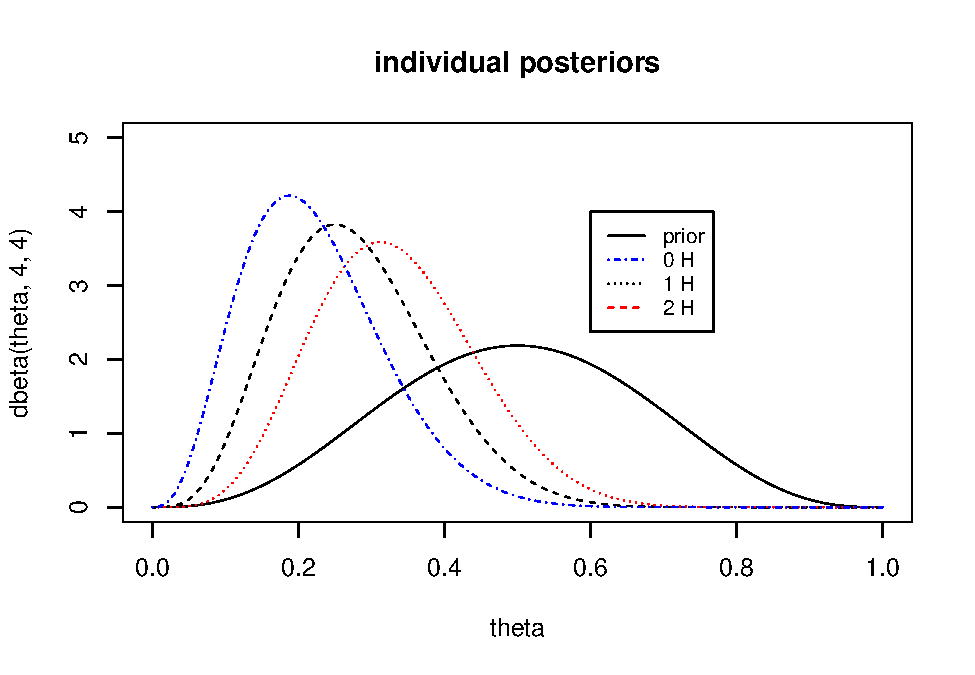
\includegraphics{_main_files/figure-latex/unnamed-chunk-11-1.pdf}

\begin{Shaded}
\begin{Highlighting}[]
\NormalTok{post}\OtherTok{\textless{}{-}}\NormalTok{ theta}\SpecialCharTok{\^{}}\DecValTok{3}\SpecialCharTok{*}\NormalTok{(}\DecValTok{1}\SpecialCharTok{{-}}\NormalTok{theta)}\SpecialCharTok{\^{}}\NormalTok{(}\DecValTok{13}\NormalTok{)}\SpecialCharTok{+}\FunctionTok{choose}\NormalTok{(}\DecValTok{10}\NormalTok{,}\DecValTok{1}\NormalTok{)}\SpecialCharTok{*}\NormalTok{theta}\SpecialCharTok{\^{}}\DecValTok{4}\SpecialCharTok{*}\NormalTok{(}\DecValTok{1}\SpecialCharTok{{-}}\NormalTok{theta)}\SpecialCharTok{\^{}}\DecValTok{12}\SpecialCharTok{+}\FunctionTok{choose}\NormalTok{(}\DecValTok{10}\NormalTok{,}\DecValTok{2}\NormalTok{)}\SpecialCharTok{*}\NormalTok{theta}\SpecialCharTok{\^{}}\DecValTok{5}\SpecialCharTok{*}\NormalTok{(}\DecValTok{1}\SpecialCharTok{{-}}\NormalTok{theta)}\SpecialCharTok{\^{}}\DecValTok{11}

\FunctionTok{plot}\NormalTok{(theta,post,}\AttributeTok{main=}\StringTok{\textquotesingle{}total posterior Y=0,1,2\textquotesingle{}}\NormalTok{)}
\end{Highlighting}
\end{Shaded}

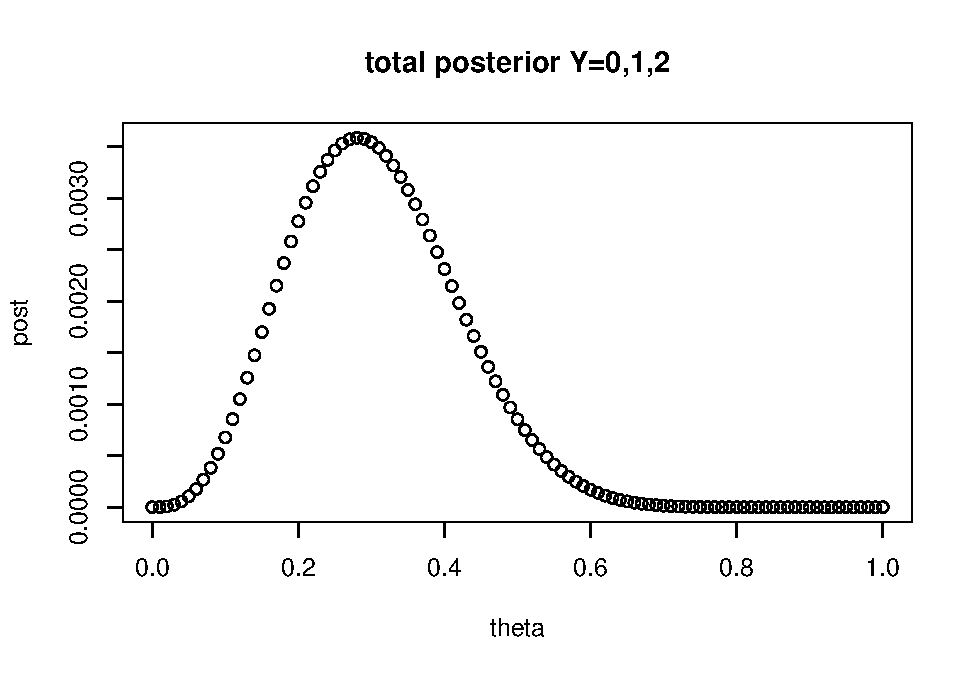
\includegraphics{_main_files/figure-latex/unnamed-chunk-11-2.pdf}

\hypertarget{normal-approximation-example}{%
\subsection*{Normal approximation example}\label{normal-approximation-example}}
\addcontentsline{toc}{subsection}{Normal approximation example}

For female births we have beta(438,544) we use the normal approximation. This replicates Gelman's Figure 2.3 (a, b)

\begin{Shaded}
\begin{Highlighting}[]
\NormalTok{  theta}\OtherTok{\textless{}{-}}\FunctionTok{seq}\NormalTok{(}\AttributeTok{from=}\FloatTok{0.001}\NormalTok{,}\AttributeTok{to=}\DecValTok{1}\NormalTok{,}\AttributeTok{by=}\FloatTok{0.01}\NormalTok{)}
  \DocumentationTok{\#\# example births}
\NormalTok{   postMean }\OtherTok{\textless{}{-}}\ControlFlowTok{function}\NormalTok{(alpha,beta,y,n)\{}
     \FunctionTok{return}\NormalTok{( (alpha}\SpecialCharTok{+}\NormalTok{y)}\SpecialCharTok{/}\NormalTok{(alpha}\SpecialCharTok{+}\NormalTok{beta}\SpecialCharTok{+}\NormalTok{n))}
\NormalTok{   \} }
\NormalTok{   postVar}\OtherTok{\textless{}{-}}\ControlFlowTok{function}\NormalTok{(alpha,beta,y,n)\{}
     \FunctionTok{return}\NormalTok{( ((alpha}\SpecialCharTok{+}\NormalTok{y)}\SpecialCharTok{*}\NormalTok{(beta}\SpecialCharTok{+}\NormalTok{n}\SpecialCharTok{{-}}\NormalTok{y))}\SpecialCharTok{/}\NormalTok{( (alpha}\SpecialCharTok{+}\NormalTok{beta}\SpecialCharTok{+}\NormalTok{n)}\SpecialCharTok{\^{}}\DecValTok{2}\SpecialCharTok{*}\NormalTok{(alpha}\SpecialCharTok{+}\NormalTok{beta}\SpecialCharTok{+}\NormalTok{n}\SpecialCharTok{+}\DecValTok{1}\NormalTok{)) )}
\NormalTok{   \}}
\NormalTok{   sdnorm}\OtherTok{\textless{}{-}}\FunctionTok{sqrt}\NormalTok{(}\FunctionTok{postVar}\NormalTok{(}\DecValTok{438}\NormalTok{,}\DecValTok{544}\NormalTok{,}\DecValTok{0}\NormalTok{,}\DecValTok{0}\NormalTok{))}
\NormalTok{   logitMean}\OtherTok{\textless{}{-}}\FunctionTok{log}\NormalTok{( }\FunctionTok{postMean}\NormalTok{(}\DecValTok{438}\NormalTok{,}\DecValTok{544}\NormalTok{,}\DecValTok{0}\NormalTok{,}\DecValTok{0}\NormalTok{)}\SpecialCharTok{/}\NormalTok{(}\DecValTok{1}\SpecialCharTok{{-}}\FunctionTok{postMean}\NormalTok{(}\DecValTok{438}\NormalTok{,}\DecValTok{544}\NormalTok{,}\DecValTok{0}\NormalTok{,}\DecValTok{0}\NormalTok{)))}
   
\NormalTok{  logitTheta}\OtherTok{\textless{}{-}}\FunctionTok{log}\NormalTok{(theta}\SpecialCharTok{/}\NormalTok{(}\DecValTok{1}\SpecialCharTok{{-}}\NormalTok{theta))}

  \FunctionTok{par}\NormalTok{(}\AttributeTok{mfrow=}\FunctionTok{c}\NormalTok{(}\DecValTok{1}\NormalTok{,}\DecValTok{2}\NormalTok{))}
    \FunctionTok{plot}\NormalTok{(theta,}\FunctionTok{dbeta}\NormalTok{(theta,}\DecValTok{438}\NormalTok{,}\DecValTok{544}\NormalTok{),}\AttributeTok{type=}\StringTok{\textquotesingle{}l\textquotesingle{}}\NormalTok{,}\AttributeTok{xlim=}\FunctionTok{c}\NormalTok{(}\FloatTok{0.35}\NormalTok{,}\FloatTok{0.55}\NormalTok{),}\AttributeTok{main=}\StringTok{"posterior beta"}\NormalTok{) }\DocumentationTok{\#\# prior}
    \FunctionTok{abline}\NormalTok{(}\AttributeTok{v=}\FloatTok{0.446}\NormalTok{,}\AttributeTok{col=}\StringTok{\textquotesingle{}red\textquotesingle{}}\NormalTok{)}
\NormalTok{  draws}\OtherTok{\textless{}{-}}\FunctionTok{rbeta}\NormalTok{(}\DecValTok{1000}\NormalTok{,}\DecValTok{438}\NormalTok{,}\DecValTok{544}\NormalTok{)}
  \FunctionTok{plot}\NormalTok{(logitTheta,}\FunctionTok{dnorm}\NormalTok{(logitTheta,}\AttributeTok{mean =}\NormalTok{logitMean, }\AttributeTok{sd=}\FunctionTok{sd}\NormalTok{(}\FunctionTok{log}\NormalTok{(draws}\SpecialCharTok{/}\NormalTok{(}\DecValTok{1}\SpecialCharTok{{-}}\NormalTok{draws))) ),}\AttributeTok{type=}\StringTok{\textquotesingle{}l\textquotesingle{}}\NormalTok{, }\AttributeTok{xlim=}\FunctionTok{c}\NormalTok{(}\SpecialCharTok{{-}}\FloatTok{0.5}\NormalTok{,}\FloatTok{0.1}\NormalTok{),}\AttributeTok{main=}\StringTok{"Normal approx."}\NormalTok{) }\DocumentationTok{\#\# prior}
    \FunctionTok{abline}\NormalTok{(}\AttributeTok{v=}\SpecialCharTok{{-}}\FloatTok{0.22}\NormalTok{,}\AttributeTok{col=}\StringTok{\textquotesingle{}red\textquotesingle{}}\NormalTok{)}
\end{Highlighting}
\end{Shaded}

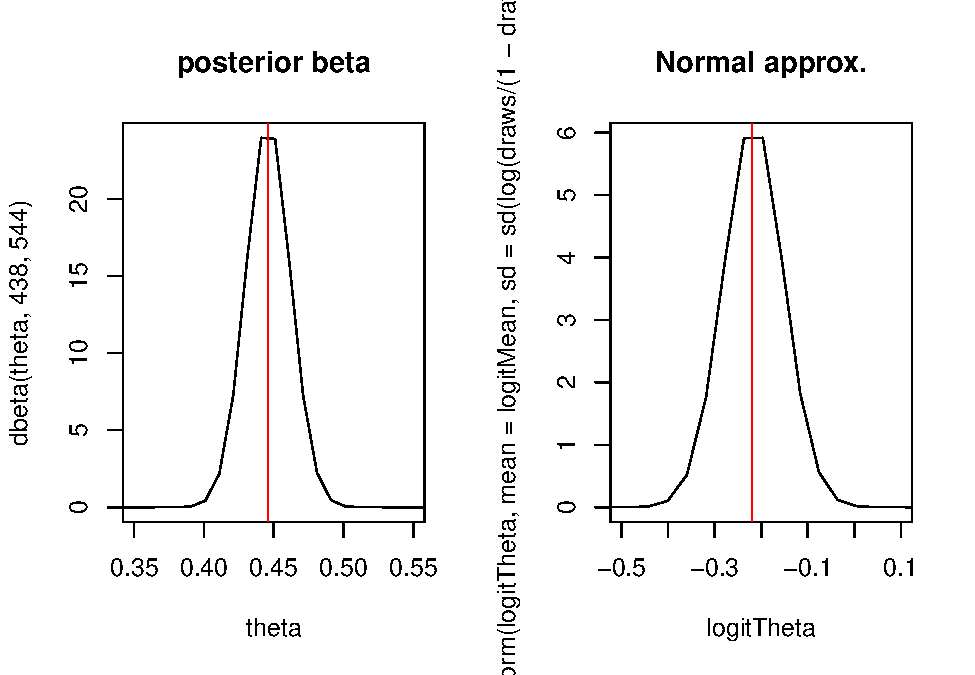
\includegraphics{_main_files/figure-latex/unnamed-chunk-12-1.pdf}

\hypertarget{question-3}{%
\subsection*{Question 3}\label{question-3}}
\addcontentsline{toc}{subsection}{Question 3}

The prior predictive distributions for the number of 6's in a fair roll, tossed 1,000 times will follow a beta distribution. Let y be the number of 6's in 1000 rolls of fair die, the probability for a 6 is 1/6, so the number of 6's (successes) in this trial is approximateley 167, and 833 failures as the prior prediction. with probabiliy of success (1/6).

We plot the beta distribution of the expected number of heads in 1000 tosses.

The normal approximation for the prior prediction uses the binomial distribution is \(\mu = n*p = 167\) and \$\sigma\^{}2 = npq \$= 138.89 \(\sim N(167, 138.89)\)

The normal approximation shows the probability of heads in a given 1000 tosses, using a non-informative prior beta(167,833) which has a prior predictive mean of \(exp(-1.79)/(1+exp(-1.79)) = 0.143\). This is not the same for number of success in 1000 tosses.

We find the probability distribution of a given success and the prior probability predictive interval follows a beta with 95\% (0.12,0.17) for hte probability of rolling a 6

\begin{Shaded}
\begin{Highlighting}[]
  \DocumentationTok{\#\# based on normal approximation sketch the distribution of y}
  \DocumentationTok{\#\# for normal we use the logit transform}
  \DocumentationTok{\#\# n = 1,000}
  \DocumentationTok{\#\# first lets construct a beta distribution.}
  \DocumentationTok{\#\# let the prior be beta(4,4) or even beta(1,1)}
\DocumentationTok{\#\# prior prediction}
\NormalTok{  theta}\OtherTok{\textless{}{-}}\FunctionTok{seq}\NormalTok{(}\AttributeTok{from=}\DecValTok{100}\NormalTok{,}\AttributeTok{to=}\DecValTok{250}\NormalTok{,}\AttributeTok{by=}\FloatTok{0.11}\NormalTok{)}
     \FunctionTok{plot}\NormalTok{(theta,}\FunctionTok{dnorm}\NormalTok{(theta,}\DecValTok{167}\NormalTok{,}\FunctionTok{sqrt}\NormalTok{(}\FloatTok{138.89}\NormalTok{)),}\AttributeTok{type=}\StringTok{\textquotesingle{}l\textquotesingle{}}\NormalTok{,}\AttributeTok{main=}\StringTok{"prior normal prediction for binomial likelihood"}\NormalTok{) }\DocumentationTok{\#\# prior}
     \FunctionTok{lines}\NormalTok{(theta,}\FunctionTok{dbinom}\NormalTok{(}\FunctionTok{round}\NormalTok{(theta),}\AttributeTok{size=}\DecValTok{1000}\NormalTok{,}\AttributeTok{prob=}\NormalTok{(}\DecValTok{1}\SpecialCharTok{/}\DecValTok{6}\NormalTok{)),}\AttributeTok{main=}\StringTok{"prior binom prediction for binomial likelihood"}\NormalTok{,}\AttributeTok{col=}\StringTok{\textquotesingle{}red\textquotesingle{}}\NormalTok{) }\DocumentationTok{\#\# prior}
\end{Highlighting}
\end{Shaded}

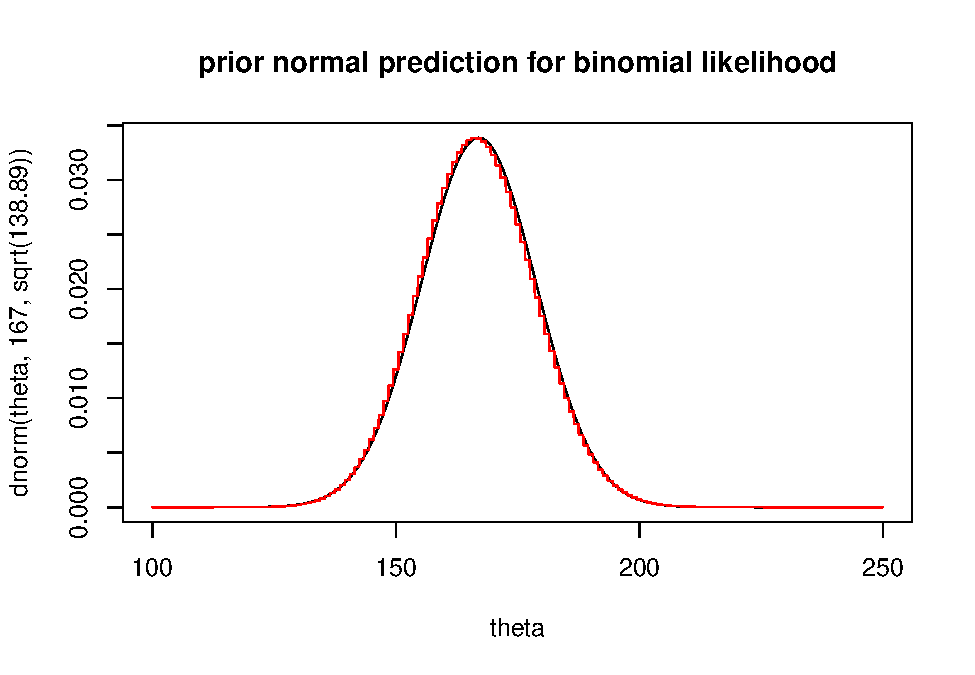
\includegraphics{_main_files/figure-latex/unnamed-chunk-13-1.pdf}

\begin{Shaded}
\begin{Highlighting}[]
  \DocumentationTok{\#\# posterior prediction (normal).}
     \DocumentationTok{\#\# assume p=1/6 we expect 167 successes under likelihood.}
\DocumentationTok{\#\# simulation     }
\NormalTok{     priordraws}\OtherTok{\textless{}{-}}\FunctionTok{sample}\NormalTok{(theta,}\AttributeTok{size=}\DecValTok{1000}\NormalTok{,}\AttributeTok{replace=}\NormalTok{T,}\AttributeTok{prob=}\FunctionTok{dnorm}\NormalTok{(theta,}\DecValTok{167}\NormalTok{,}\FunctionTok{sqrt}\NormalTok{(}\FloatTok{138.89}\NormalTok{)))}
\NormalTok{     priorpred}\OtherTok{\textless{}{-}}\FunctionTok{rnorm}\NormalTok{(}\DecValTok{1000}\NormalTok{,}\AttributeTok{mean=}\NormalTok{priordraws,}\AttributeTok{sd=}\FunctionTok{sqrt}\NormalTok{(}\FloatTok{138.89}\NormalTok{))}
     \DocumentationTok{\#\# prior prediction interval}
     \FunctionTok{quantile}\NormalTok{(priorpred,}\FunctionTok{c}\NormalTok{(}\FloatTok{0.05}\NormalTok{,}\FloatTok{0.25}\NormalTok{,}\FloatTok{0.5}\NormalTok{,}\FloatTok{0.75}\NormalTok{,}\FloatTok{0.95}\NormalTok{))}
\end{Highlighting}
\end{Shaded}

\begin{verbatim}
##       5%      25%      50%      75%      95% 
## 138.3998 154.2043 166.2336 178.5477 195.1530
\end{verbatim}

\begin{Shaded}
\begin{Highlighting}[]
     \FunctionTok{qnorm}\NormalTok{(}\FunctionTok{c}\NormalTok{(}\FloatTok{0.05}\NormalTok{,}\FloatTok{0.25}\NormalTok{,}\FloatTok{0.5}\NormalTok{,}\FloatTok{0.75}\NormalTok{,}\FloatTok{0.95}\NormalTok{),}\DecValTok{167}\NormalTok{,}\FunctionTok{sqrt}\NormalTok{(}\FloatTok{138.89}\NormalTok{))}
\end{Highlighting}
\end{Shaded}

\begin{verbatim}
## [1] 147.6151 159.0510 167.0000 174.9490 186.3849
\end{verbatim}

\hypertarget{question-4}{%
\subsection*{Question 4}\label{question-4}}
\addcontentsline{toc}{subsection}{Question 4}

We have a mixture of 3 normal distributions, and show the central intervals for 5,25,50,75, and 95\(\%\) predictive probabilities. The question gives \(\theta\) as the probability of a 6 on a die, possibly unfair, in 1,000 tosses. we have \(\theta= 1/12,1/6, 1/4\) types of biased die. Using the normal approximation, the predictive prior probability is \(\sum_{\theta}p(\theta)p(y| \theta)\) where the likelihood is approximated using a normal distribution \(\mu = n*\theta_i, \sigma = n*\theta_i(1-\theta_i)\)

\begin{Shaded}
\begin{Highlighting}[]
\NormalTok{x}\OtherTok{\textless{}{-}}\FunctionTok{seq}\NormalTok{(}\DecValTok{0}\NormalTok{,}\DecValTok{1000}\NormalTok{)}\SpecialCharTok{{-}}\FloatTok{0.5} \CommentTok{\# continuity correction.}
\NormalTok{theta}\OtherTok{\textless{}{-}}\FunctionTok{c}\NormalTok{(}\DecValTok{1}\SpecialCharTok{/}\DecValTok{12}\NormalTok{,}\DecValTok{1}\SpecialCharTok{/}\DecValTok{6}\NormalTok{,}\DecValTok{1}\SpecialCharTok{/}\DecValTok{4}\NormalTok{)}
\NormalTok{n}\OtherTok{=}\DecValTok{1000}

\NormalTok{a}\OtherTok{\textless{}{-}}\FunctionTok{dnorm}\NormalTok{(x,}\AttributeTok{mean=}\NormalTok{n}\SpecialCharTok{*}\NormalTok{theta[}\DecValTok{1}\NormalTok{],}\AttributeTok{sd=}\FunctionTok{sqrt}\NormalTok{(n}\SpecialCharTok{*}\NormalTok{theta[}\DecValTok{1}\NormalTok{]}\SpecialCharTok{*}\NormalTok{(}\DecValTok{1}\SpecialCharTok{{-}}\NormalTok{theta[}\DecValTok{1}\NormalTok{]))  )}
\NormalTok{b}\OtherTok{\textless{}{-}}\FunctionTok{dnorm}\NormalTok{(x,}\AttributeTok{mean=}\NormalTok{n}\SpecialCharTok{*}\NormalTok{theta[}\DecValTok{2}\NormalTok{],}\AttributeTok{sd=}\FunctionTok{sqrt}\NormalTok{(n}\SpecialCharTok{*}\NormalTok{theta[}\DecValTok{2}\NormalTok{]}\SpecialCharTok{*}\NormalTok{(}\DecValTok{1}\SpecialCharTok{{-}}\NormalTok{theta[}\DecValTok{2}\NormalTok{]))  )}
\NormalTok{c}\OtherTok{\textless{}{-}}\FunctionTok{dnorm}\NormalTok{(x,}\AttributeTok{mean=}\NormalTok{n}\SpecialCharTok{*}\NormalTok{theta[}\DecValTok{3}\NormalTok{],}\AttributeTok{sd=}\FunctionTok{sqrt}\NormalTok{(n}\SpecialCharTok{*}\NormalTok{theta[}\DecValTok{3}\NormalTok{]}\SpecialCharTok{*}\NormalTok{(}\DecValTok{1}\SpecialCharTok{{-}}\NormalTok{theta[}\DecValTok{3}\NormalTok{]))  )}

 \DocumentationTok{\#\# posterior computation}
 \DocumentationTok{\#\#p(y) =  p(y| theta1 )*p(theta1)+ p(y| theta2 )*p(theta2)+ p(y| theta3 )*p(theta3)}
 \CommentTok{\# total law of probability}
\NormalTok{mypost}\OtherTok{\textless{}{-}}\NormalTok{a}\SpecialCharTok{*}\FloatTok{0.25}\SpecialCharTok{+}\NormalTok{b}\SpecialCharTok{*}\FloatTok{0.5}\SpecialCharTok{+}\NormalTok{c}\SpecialCharTok{*}\FloatTok{0.25}

\DocumentationTok{\#\# prior pred  p(y) = p(y|theta)*p(theta) / p(theta| y)}
\NormalTok{mypri}\OtherTok{\textless{}{-}}\NormalTok{mypost}

\FunctionTok{sum}\NormalTok{(mypri) }\DocumentationTok{\#\# sums to 1 it is a distribution}
\end{Highlighting}
\end{Shaded}

\begin{verbatim}
## [1] 1
\end{verbatim}

\begin{Shaded}
\begin{Highlighting}[]
 \FunctionTok{par}\NormalTok{(}\AttributeTok{mfrow=}\FunctionTok{c}\NormalTok{(}\DecValTok{3}\NormalTok{,}\DecValTok{2}\NormalTok{))}
\FunctionTok{plot}\NormalTok{(x,mypri,}\AttributeTok{type=}\StringTok{\textquotesingle{}l\textquotesingle{}}\NormalTok{,}\AttributeTok{main=}\StringTok{\textquotesingle{}predictive prior number of heads\textquotesingle{}}\NormalTok{)}



\NormalTok{data}\OtherTok{\textless{}{-}}\FunctionTok{data.frame}\NormalTok{(}\AttributeTok{x=}\NormalTok{x,}\AttributeTok{p=}\NormalTok{mypri)}

\DocumentationTok{\#\# highest probability interval}
\CommentTok{\# 95\%}

\FunctionTok{plot}\NormalTok{(x,mypri,}\AttributeTok{type=}\StringTok{\textquotesingle{}l\textquotesingle{}}\NormalTok{,}\AttributeTok{main=}\StringTok{\textquotesingle{} 95\% predictive prior number of heads\textquotesingle{}}\NormalTok{)}
\FunctionTok{abline}\NormalTok{(}\AttributeTok{v=}\FunctionTok{max}\NormalTok{(data[}\FunctionTok{which}\NormalTok{(}\FunctionTok{cumsum}\NormalTok{(data}\SpecialCharTok{$}\NormalTok{p)}\SpecialCharTok{\textless{}}\FloatTok{0.025}\NormalTok{),}\DecValTok{1}\NormalTok{])}
\NormalTok{)}
\FunctionTok{abline}\NormalTok{(}\AttributeTok{v=}\FunctionTok{max}\NormalTok{(data[}\FunctionTok{which}\NormalTok{(}\DecValTok{1}\SpecialCharTok{{-}}\FunctionTok{cumsum}\NormalTok{(data}\SpecialCharTok{$}\NormalTok{p)}\SpecialCharTok{\textgreater{}}\FloatTok{0.025}\NormalTok{),}\DecValTok{1}\NormalTok{]))}

\FunctionTok{plot}\NormalTok{(x,mypri,}\AttributeTok{type=}\StringTok{\textquotesingle{}l\textquotesingle{}}\NormalTok{,}\AttributeTok{main=}\StringTok{\textquotesingle{}75\% predictive prior number of heads\textquotesingle{}}\NormalTok{)}
\FunctionTok{abline}\NormalTok{(}\AttributeTok{v=}\FunctionTok{max}\NormalTok{(data[}\FunctionTok{which}\NormalTok{(}\FunctionTok{cumsum}\NormalTok{(data}\SpecialCharTok{$}\NormalTok{p)}\SpecialCharTok{\textless{}}\FloatTok{0.125}\NormalTok{),}\DecValTok{1}\NormalTok{]))}
\FunctionTok{abline}\NormalTok{(}\AttributeTok{v=}\FunctionTok{max}\NormalTok{(data[}\FunctionTok{which}\NormalTok{(}\DecValTok{1}\SpecialCharTok{{-}}\FunctionTok{cumsum}\NormalTok{(data}\SpecialCharTok{$}\NormalTok{p)}\SpecialCharTok{\textgreater{}}\FloatTok{0.125}\NormalTok{),}\DecValTok{1}\NormalTok{])}
\NormalTok{)}

\FunctionTok{plot}\NormalTok{(x,mypri,}\AttributeTok{type=}\StringTok{\textquotesingle{}l\textquotesingle{}}\NormalTok{,}\AttributeTok{main=}\StringTok{\textquotesingle{}50\% predictive prior number of heads\textquotesingle{}}\NormalTok{)}
\FunctionTok{abline}\NormalTok{(}\AttributeTok{v=}\FunctionTok{max}\NormalTok{(data[}\FunctionTok{which}\NormalTok{(}\FunctionTok{cumsum}\NormalTok{(data}\SpecialCharTok{$}\NormalTok{p)}\SpecialCharTok{\textless{}}\FloatTok{0.25}\NormalTok{),}\DecValTok{1}\NormalTok{]))}
\FunctionTok{abline}\NormalTok{(}\AttributeTok{v=}\FunctionTok{max}\NormalTok{(data[}\FunctionTok{which}\NormalTok{(}\DecValTok{1}\SpecialCharTok{{-}}\FunctionTok{cumsum}\NormalTok{(data}\SpecialCharTok{$}\NormalTok{p)}\SpecialCharTok{\textgreater{}}\FloatTok{0.25}\NormalTok{),}\DecValTok{1}\NormalTok{])}
\NormalTok{)}

\FunctionTok{plot}\NormalTok{(x,mypri,}\AttributeTok{type=}\StringTok{\textquotesingle{}l\textquotesingle{}}\NormalTok{,}\AttributeTok{main=}\StringTok{\textquotesingle{}25\% predictive prior number of heads\textquotesingle{}}\NormalTok{)}
\FunctionTok{abline}\NormalTok{(}\AttributeTok{v=}\FunctionTok{max}\NormalTok{(data[}\FunctionTok{which}\NormalTok{(}\FunctionTok{cumsum}\NormalTok{(data}\SpecialCharTok{$}\NormalTok{p)}\SpecialCharTok{\textless{}}\FloatTok{0.375}\NormalTok{),}\DecValTok{1}\NormalTok{]))}
\FunctionTok{abline}\NormalTok{(}\AttributeTok{v=}\FunctionTok{max}\NormalTok{(data[}\FunctionTok{which}\NormalTok{(}\DecValTok{1}\SpecialCharTok{{-}}\FunctionTok{cumsum}\NormalTok{(data}\SpecialCharTok{$}\NormalTok{p)}\SpecialCharTok{\textgreater{}}\FloatTok{0.375}\NormalTok{),}\DecValTok{1}\NormalTok{])}
\NormalTok{)}

\FunctionTok{plot}\NormalTok{(x,mypri,}\AttributeTok{type=}\StringTok{\textquotesingle{}l\textquotesingle{}}\NormalTok{,}\AttributeTok{main=}\StringTok{\textquotesingle{}5\% predictive prior number of heads\textquotesingle{}}\NormalTok{)}
\FunctionTok{abline}\NormalTok{(}\AttributeTok{v=}\FunctionTok{max}\NormalTok{(data[}\FunctionTok{which}\NormalTok{(}\FunctionTok{cumsum}\NormalTok{(data}\SpecialCharTok{$}\NormalTok{p)}\SpecialCharTok{\textless{}}\FloatTok{0.475}\NormalTok{),}\DecValTok{1}\NormalTok{]))}
\FunctionTok{abline}\NormalTok{(}\AttributeTok{v=}\FunctionTok{max}\NormalTok{(data[}\FunctionTok{which}\NormalTok{(}\DecValTok{1}\SpecialCharTok{{-}}\FunctionTok{cumsum}\NormalTok{(data}\SpecialCharTok{$}\NormalTok{p)}\SpecialCharTok{\textgreater{}}\FloatTok{0.475}\NormalTok{),}\DecValTok{1}\NormalTok{])}
\NormalTok{)}
\end{Highlighting}
\end{Shaded}

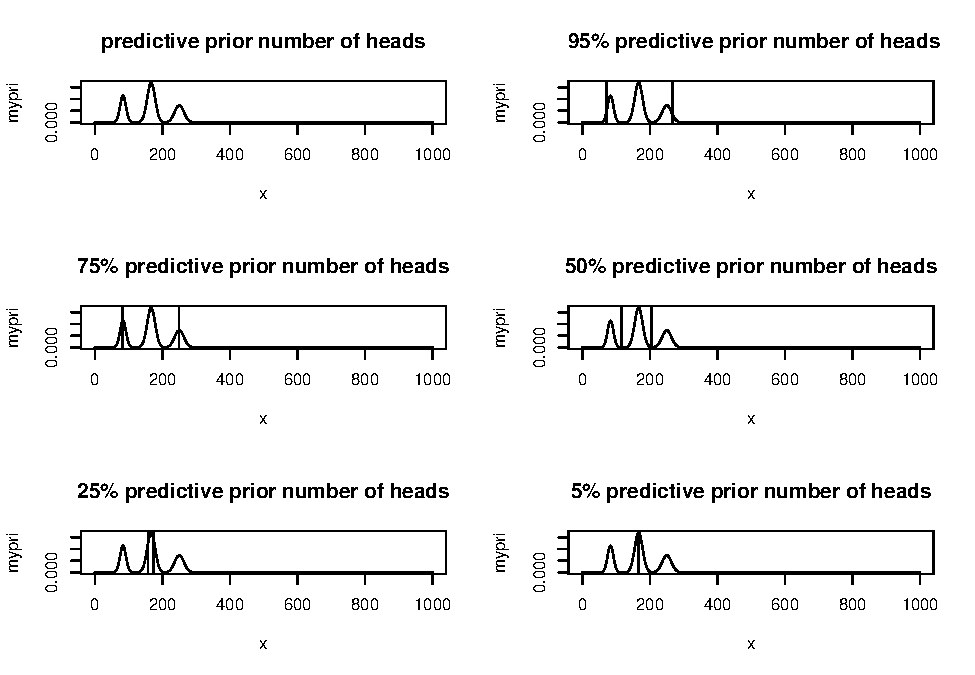
\includegraphics{_main_files/figure-latex/unnamed-chunk-14-1.pdf}

\hypertarget{question-7}{%
\subsection*{Question 7}\label{question-7}}
\addcontentsline{toc}{subsection}{Question 7}

\begin{itemize}
\item
  \begin{enumerate}
  \def\labelenumi{(\alph{enumi})}
  \tightlist
  \item
    for the binomial likelihood \(y\sim Bin(n,\theta)\), show that p(\(\theta)\propto \theta^-1(1-\theta)^-1\) is the uniform prior for the natural parameter of the exponential family.
  \end{enumerate}
\item
  first we write the binomial likelihood in exponential family form, note that we are not deriving the posterior of any function, but just studying the likelihood.
\end{itemize}

\[
\begin{aligned}
p(y|\theta) &= \theta^y(1-\theta)^{n-y}\\
\implies log(p)&= ylog(\theta/(1-\theta))+nlog(1-\theta) \\
\implies p(y|\theta) &= exp(y*log(\theta/(1-\theta)))*g(\theta)\\
\text{hence } \phi(\theta)= log(\theta/1-\theta), \text{  and we're given uniformity  } p(\phi(\theta))\propto 1\\
\end{aligned}
\]
Inverting \(\phi(\theta)=log(\theta/1-\theta)\) yields \(\theta=\frac{e^\phi}{1+e^\phi}\) and we know that p(\(\phi)\propto 1\). Using the jacobian we can derive \(p(\theta)=p(\phi)\frac{d\phi}{d\theta}\) shown as

\[
\begin{aligned}
p(\theta)&=p(\phi)\frac{d\phi}{d\theta}\\
&= p(\phi)d/d\theta (log(\theta/1-\theta))\\
&\propto (1) (1-\theta / \theta)(1/(1-\theta)^2) \\
&= 1/\theta *(1/1-\theta) 
\end{aligned}
\]

\hypertarget{question-8-normal-distribution-with-unknown-mean}{%
\subsection*{Question 8 (Normal distribution with unknown mean)}\label{question-8-normal-distribution-with-unknown-mean}}
\addcontentsline{toc}{subsection}{Question 8 (Normal distribution with unknown mean)}

A random sample of n students is drawn from a large population, and weights are measured. The average height of the n sampled students is \(\bar{y}= 150\) lbs. Assume the weights in the population are normally distribution with unknown mean, \(\theta\), and known standard deviation 20 lbs. Suppose the prior for \(\theta \sim N(180, 40^2)\)

\begin{itemize}
\item
  \begin{enumerate}
  \def\labelenumi{(\alph{enumi})}
  \tightlist
  \item
    For known variance, the limit of the posterior is \(p(\theta,y)\approx N(\theta| \bar{y}, \sigma^2/n)\). And the direct formulation is \(p(\theta | \bar{y})= N(\theta | \mu_n,\tau_n^2).\) using equations 2.12.
  \end{enumerate}
\item
  \begin{enumerate}
  \def\labelenumi{(\alph{enumi})}
  \setcounter{enumi}{1}
  \tightlist
  \item
    For a posterior predictive interval, the marginal distribution for new data \(p(\tilde{y} | y) \sim N(\mu_n, \sigma^2+\tau_n^2)\)
  \end{enumerate}
\end{itemize}

\begin{Shaded}
\begin{Highlighting}[]
\NormalTok{mu\_n}\OtherTok{\textless{}{-}}\ControlFlowTok{function}\NormalTok{(mu0,ybar,n,tau02,sigma2)\{}
\NormalTok{  mun}\OtherTok{\textless{}{-}}\NormalTok{ (mu0}\SpecialCharTok{/}\NormalTok{tau02 }\SpecialCharTok{+}\NormalTok{ (ybar}\SpecialCharTok{*}\NormalTok{n)}\SpecialCharTok{/}\NormalTok{sigma2)}\SpecialCharTok{/}\NormalTok{(}\DecValTok{1}\SpecialCharTok{/}\NormalTok{tau02 }\SpecialCharTok{+}\NormalTok{ n}\SpecialCharTok{/}\NormalTok{sigma2)}
  \FunctionTok{return}\NormalTok{(mun)}
\NormalTok{\}}
\NormalTok{taun2}\OtherTok{\textless{}{-}}\ControlFlowTok{function}\NormalTok{(tau02,n,sigma2)\{}
\NormalTok{  inv.taun2}\OtherTok{\textless{}{-}} \DecValTok{1}\SpecialCharTok{/}\NormalTok{tau02 }\SpecialCharTok{+}\NormalTok{n}\SpecialCharTok{/}\NormalTok{sigma2}
  \FunctionTok{return}\NormalTok{(}\DecValTok{1}\SpecialCharTok{/}\NormalTok{inv.taun2)}
\NormalTok{\}}
\end{Highlighting}
\end{Shaded}

\begin{itemize}
\item
  \begin{enumerate}
  \def\labelenumi{(\alph{enumi})}
  \setcounter{enumi}{2}
  \tightlist
  \item
    Here we give the posterior interval and predictive interval for n=10
  \end{enumerate}
\end{itemize}

\begin{Shaded}
\begin{Highlighting}[]
\NormalTok{ybar}\OtherTok{=}\DecValTok{150}
\NormalTok{sigma2}\OtherTok{=}\DecValTok{20}\SpecialCharTok{\^{}}\DecValTok{2}
\NormalTok{mu0}\OtherTok{=}\DecValTok{180}
\NormalTok{  tau02}\OtherTok{=}\DecValTok{40}\SpecialCharTok{\^{}}\DecValTok{2}
\NormalTok{  n}\OtherTok{=}\DecValTok{10}

\DocumentationTok{\#\# posterior interval n=10}
  \CommentTok{\#lower\textless{}{-}round(qnorm(0.025,mu\_n(mu0,ybar,tau02,10,sigma2),sd=sqrt(taun2(tau02,10,sigma2))),2)}
\NormalTok{    upper}\OtherTok{\textless{}{-}}\FunctionTok{round}\NormalTok{(}\FunctionTok{qnorm}\NormalTok{(}\FunctionTok{c}\NormalTok{(}\FloatTok{0.025}\NormalTok{,}\FloatTok{0.975}\NormalTok{),}\FunctionTok{mu\_n}\NormalTok{(mu0,ybar,tau02,}\DecValTok{10}\NormalTok{,sigma2),}\AttributeTok{sd=}\FunctionTok{sqrt}\NormalTok{(}\FunctionTok{taun2}\NormalTok{(tau02,}\DecValTok{10}\NormalTok{,sigma2))),}\DecValTok{2}\NormalTok{)}

\FunctionTok{message}\NormalTok{(}\StringTok{"posterior interval n=10: "}\NormalTok{,upper[}\DecValTok{1}\NormalTok{],}\StringTok{" "}\NormalTok{,upper[}\DecValTok{2}\NormalTok{])}
\end{Highlighting}
\end{Shaded}

\begin{verbatim}
## posterior interval n=10: 138.49 162.98
\end{verbatim}

\begin{Shaded}
\begin{Highlighting}[]
\DocumentationTok{\#\# posterior predictive interval}
\NormalTok{  upper2}\OtherTok{\textless{}{-}}\FunctionTok{round}\NormalTok{(}\FunctionTok{qnorm}\NormalTok{(}\FunctionTok{c}\NormalTok{(}\FloatTok{0.025}\NormalTok{,}\FloatTok{0.975}\NormalTok{),}\FunctionTok{mu\_n}\NormalTok{(mu0,ybar,tau02,}\DecValTok{10}\NormalTok{,sigma2),}\AttributeTok{sd=}\FunctionTok{sqrt}\NormalTok{(}\FunctionTok{taun2}\NormalTok{(tau02,}\DecValTok{10}\NormalTok{,sigma2)}\SpecialCharTok{+}\NormalTok{sigma2) ),}\DecValTok{2}\NormalTok{)}

\FunctionTok{message}\NormalTok{(}\StringTok{"posterior predictive interval n=10: "}\NormalTok{,upper2[}\DecValTok{1}\NormalTok{],}\StringTok{" "}\NormalTok{,upper2[}\DecValTok{2}\NormalTok{])}
\end{Highlighting}
\end{Shaded}

\begin{verbatim}
## posterior predictive interval n=10: 109.66 191.8
\end{verbatim}

\begin{itemize}
\item
  \begin{enumerate}
  \def\labelenumi{(\alph{enumi})}
  \setcounter{enumi}{3}
  \tightlist
  \item
    the posterior and predictive for n=100
  \end{enumerate}
\end{itemize}

\begin{Shaded}
\begin{Highlighting}[]
\NormalTok{ lower}\OtherTok{\textless{}{-}}\FunctionTok{round}\NormalTok{(}\FunctionTok{qnorm}\NormalTok{(}\FloatTok{0.025}\NormalTok{,}\FunctionTok{mu\_n}\NormalTok{(mu0,ybar,tau02,}\DecValTok{100}\NormalTok{,sigma2),}\AttributeTok{sd=}\FunctionTok{sqrt}\NormalTok{(}\FunctionTok{taun2}\NormalTok{(tau02,}\DecValTok{100}\NormalTok{,sigma2))),}\DecValTok{2}\NormalTok{)}
\NormalTok{    upper}\OtherTok{\textless{}{-}}\FunctionTok{round}\NormalTok{(}\FunctionTok{qnorm}\NormalTok{(}\FloatTok{0.975}\NormalTok{,}\FunctionTok{mu\_n}\NormalTok{(mu0,ybar,tau02,}\DecValTok{100}\NormalTok{,sigma2),}\AttributeTok{sd=}\FunctionTok{sqrt}\NormalTok{(}\FunctionTok{taun2}\NormalTok{(tau02,}\DecValTok{100}\NormalTok{,sigma2))),}\DecValTok{2}\NormalTok{)}

\FunctionTok{message}\NormalTok{(}\StringTok{"posterior interval n=100: "}\NormalTok{,lower,}\StringTok{" "}\NormalTok{,upper)}
\end{Highlighting}
\end{Shaded}

\begin{verbatim}
## posterior interval n=100: 146.16 153.99
\end{verbatim}

\begin{Shaded}
\begin{Highlighting}[]
 \DocumentationTok{\#\# this approximately equals the limit}
\FunctionTok{print}\NormalTok{(}\StringTok{"The asymptotic approximation"}\NormalTok{)}
\end{Highlighting}
\end{Shaded}

\begin{verbatim}
## [1] "The asymptotic approximation"
\end{verbatim}

\begin{Shaded}
\begin{Highlighting}[]
 \FunctionTok{qnorm}\NormalTok{(}\FunctionTok{c}\NormalTok{(}\FloatTok{0.025}\NormalTok{,}\FloatTok{0.975}\NormalTok{),}\AttributeTok{mean=}\DecValTok{150}\NormalTok{, sigma2}\SpecialCharTok{/}\DecValTok{100}\NormalTok{)}
\end{Highlighting}
\end{Shaded}

\begin{verbatim}
## [1] 142.1601 157.8399
\end{verbatim}

\begin{Shaded}
\begin{Highlighting}[]
\DocumentationTok{\#\# posterior predictive interval}
\NormalTok{ lower2}\OtherTok{\textless{}{-}}\FunctionTok{round}\NormalTok{(}\FunctionTok{qnorm}\NormalTok{(}\FloatTok{0.025}\NormalTok{,}\FunctionTok{mu\_n}\NormalTok{(mu0,ybar,tau02,}\DecValTok{100}\NormalTok{,sigma2),}\AttributeTok{sd=}\FunctionTok{sqrt}\NormalTok{(}\FunctionTok{taun2}\NormalTok{(tau02,}\DecValTok{100}\NormalTok{,sigma2)}\SpecialCharTok{+}\NormalTok{sigma2) ),}\DecValTok{2}\NormalTok{)}
\NormalTok{    upper2}\OtherTok{\textless{}{-}}\FunctionTok{round}\NormalTok{(}\FunctionTok{qnorm}\NormalTok{(}\FloatTok{0.975}\NormalTok{,}\FunctionTok{mu\_n}\NormalTok{(mu0,ybar,tau02,}\DecValTok{100}\NormalTok{,sigma2),}\AttributeTok{sd=}\FunctionTok{sqrt}\NormalTok{(}\FunctionTok{taun2}\NormalTok{(tau02,}\DecValTok{100}\NormalTok{,sigma2)}\SpecialCharTok{+}\NormalTok{sigma2) ),}\DecValTok{2}\NormalTok{)}

\FunctionTok{message}\NormalTok{(}\StringTok{"posterior predictive interval n=100: "}\NormalTok{,lower2,}\StringTok{" "}\NormalTok{,upper2)}
\end{Highlighting}
\end{Shaded}

\begin{verbatim}
## posterior predictive interval n=100: 110.68 189.47
\end{verbatim}

\hypertarget{question-10}{%
\subsection*{Question 10}\label{question-10}}
\addcontentsline{toc}{subsection}{Question 10}

Suppose there are N cable cars numbered sequentially 1 to N. You see a car at random labeled 203 and wish to estimate N. (a) assume the prior follows Geo(1/100) what is the posterior for N?

\begin{itemize}
\item
  \begin{enumerate}
  \def\labelenumi{(\alph{enumi})}
  \tightlist
  \item
    The car X=203 was observed, and the likelihood of this observation (data) is uniform p(\(X|N=203)=1/N\) which assumes each car is equally likely. So the posterior \(p(N|X) = (1/N)(1/100)(99/100)^{N-1}\). So the posterior is proportional to \((1/N)(99/100)^{N-1}\) with \(N\geq 203\).
  \end{enumerate}
\item
  what is the posterior mean and std. deviation for N?.
  we use Bayes' theorem \(p(N|X) = \frac{p(X|N)p(N)}{p(X)}\). And use a computer to approximation p(X) which is approximately 0.0471 (ignoring constant).
  the infinite series \(\sum_{n=203}^\infty (1/n)(99/100)^{n-1}\) converges by using the ratio test with \(\rho<1\) to \$\approx 0.0471.
  The posterior mean and standard deviation is 279.09 a.nd 79.96, which was evaluated using the posterior distribution \(p(N|X)\) defined as
  \[
   p(N|X) \propto \frac{(1/N)(99/100)^{N-1}}{p(X)}  
  \]
\end{itemize}

\begin{Shaded}
\begin{Highlighting}[]
\NormalTok{ totalSum}\OtherTok{=}\DecValTok{0}
 
 \ControlFlowTok{for}\NormalTok{(i }\ControlFlowTok{in} \DecValTok{203}\SpecialCharTok{:}\DecValTok{30000}\NormalTok{)\{}
\NormalTok{  sum\_i}\OtherTok{=}\NormalTok{ (}\DecValTok{1}\SpecialCharTok{/}\NormalTok{i)}\SpecialCharTok{*}\NormalTok{(}\DecValTok{99}\SpecialCharTok{/}\DecValTok{100}\NormalTok{)}\SpecialCharTok{\^{}}\NormalTok{(i}\DecValTok{{-}1}\NormalTok{)}
\NormalTok{  totalSum}\OtherTok{=}\NormalTok{ totalSum}\SpecialCharTok{+}\NormalTok{sum\_i}
  
\NormalTok{ \}}
 \FunctionTok{print}\NormalTok{(totalSum)}
\end{Highlighting}
\end{Shaded}

\begin{verbatim}
## [1] 0.04705084
\end{verbatim}

\begin{Shaded}
\begin{Highlighting}[]
 \DocumentationTok{\#\# approximate the distribution}
\NormalTok{ px}\OtherTok{\textless{}{-}}\NormalTok{totalSum}
\NormalTok{ X}\OtherTok{\textless{}{-}}\FunctionTok{seq}\NormalTok{(}\DecValTok{203}\NormalTok{,}\DecValTok{300000}\NormalTok{)}
 
\NormalTok{ dpx}\OtherTok{\textless{}{-}}\ControlFlowTok{function}\NormalTok{(N,px)\{}
\NormalTok{   dd}\OtherTok{\textless{}{-}}\NormalTok{ (}\DecValTok{1}\SpecialCharTok{/}\NormalTok{px)}\SpecialCharTok{*}\NormalTok{(}\DecValTok{1}\SpecialCharTok{/}\NormalTok{N)}\SpecialCharTok{*}\NormalTok{(}\DecValTok{99}\SpecialCharTok{/}\DecValTok{100}\NormalTok{)}\SpecialCharTok{\^{}}\NormalTok{(N}\DecValTok{{-}1}\NormalTok{)}
   
   \FunctionTok{return}\NormalTok{(dd)}
\NormalTok{ \}}
 \DocumentationTok{\#\# the posterior mean is}
  \DocumentationTok{\#\# E(X) = x*f(x)}
\NormalTok{ postMean}\OtherTok{\textless{}{-}}\ControlFlowTok{function}\NormalTok{(N,px)\{}
\NormalTok{   fx}\OtherTok{\textless{}{-}} \FunctionTok{dpx}\NormalTok{(N,px)}
\NormalTok{   ex}\OtherTok{\textless{}{-}}\NormalTok{ N}\SpecialCharTok{*}\NormalTok{fx}
   \FunctionTok{return}\NormalTok{(ex)}
\NormalTok{ \}}
\NormalTok{  EX}\OtherTok{\textless{}{-}}\FunctionTok{sum}\NormalTok{(}\FunctionTok{postMean}\NormalTok{(X,px))}
  
\DocumentationTok{\#\# posterior variance}
   \DocumentationTok{\#\# VX = EX\^{}2 {-} (EX)\^{}2}
\NormalTok{postMean.sq}\OtherTok{\textless{}{-}}\ControlFlowTok{function}\NormalTok{(N,px)\{}
\NormalTok{   fx}\OtherTok{\textless{}{-}} \FunctionTok{dpx}\NormalTok{(N,px)}
\NormalTok{   ex2}\OtherTok{\textless{}{-}}\NormalTok{ N}\SpecialCharTok{*}\NormalTok{N}\SpecialCharTok{*}\NormalTok{fx}
   \FunctionTok{return}\NormalTok{(ex2)}
\NormalTok{\}}
 \DocumentationTok{\#\# the variance term has to be evaluated at smaller limit to avoid overflow}
\NormalTok{sdX}\OtherTok{\textless{}{-}}\FunctionTok{sqrt}\NormalTok{(}\FunctionTok{sum}\NormalTok{(}\FunctionTok{postMean.sq}\NormalTok{(}\FunctionTok{seq}\NormalTok{(}\DecValTok{203}\NormalTok{,}\DecValTok{35000}\NormalTok{),px))}\SpecialCharTok{{-}}\NormalTok{(EX)}\SpecialCharTok{\^{}}\DecValTok{2}\NormalTok{)}
\FunctionTok{message}\NormalTok{(}\StringTok{"posterior mean and sd is:"}\NormalTok{, }\FunctionTok{round}\NormalTok{(EX,}\DecValTok{2}\NormalTok{),}\StringTok{" "}\NormalTok{,}\FunctionTok{round}\NormalTok{(sdX,}\DecValTok{2}\NormalTok{))}
\end{Highlighting}
\end{Shaded}

\begin{verbatim}
## posterior mean and sd is:279.09 79.96
\end{verbatim}

\begin{itemize}
\item
  \begin{enumerate}
  \def\labelenumi{(\alph{enumi})}
  \setcounter{enumi}{1}
  \tightlist
  \item
    we use a simulation to estimate the posterior. We sample with replacement, with a distribution size equal to a large number (N), with probability of observing a number equal to the posterior distribution. The empirial mean and std.dev are 280.5, and 80.9
  \end{enumerate}
\end{itemize}

\begin{Shaded}
\begin{Highlighting}[]
\NormalTok{ N}\OtherTok{\textless{}{-}}\DecValTok{203}\SpecialCharTok{:}\DecValTok{100000}
\NormalTok{ Nsim}\OtherTok{\textless{}{-}}\DecValTok{10000}
\NormalTok{ unnorm.post}\OtherTok{\textless{}{-}}\NormalTok{(}\DecValTok{1}\SpecialCharTok{/}\NormalTok{N)}\SpecialCharTok{*}\NormalTok{(}\DecValTok{99}\SpecialCharTok{/}\DecValTok{100}\NormalTok{)}\SpecialCharTok{\^{}}\NormalTok{(N}\DecValTok{{-}10}\NormalTok{)}
 \FunctionTok{mean}\NormalTok{(}\FunctionTok{sample}\NormalTok{(N,}\AttributeTok{size=}\NormalTok{Nsim,}\AttributeTok{prob=}\NormalTok{unnorm.post,}\AttributeTok{replace=}\NormalTok{T))}
\end{Highlighting}
\end{Shaded}

\begin{verbatim}
## [1] 278.1989
\end{verbatim}

\begin{Shaded}
\begin{Highlighting}[]
 \FunctionTok{sd}\NormalTok{(}\FunctionTok{sample}\NormalTok{(N,}\AttributeTok{size=}\NormalTok{Nsim,}\AttributeTok{prob=}\NormalTok{unnorm.post,}\AttributeTok{replace=}\NormalTok{T))}
\end{Highlighting}
\end{Shaded}

\begin{verbatim}
## [1] 80.04754
\end{verbatim}

\begin{itemize}
\item
  \begin{enumerate}
  \def\labelenumi{(\alph{enumi})}
  \setcounter{enumi}{2}
  \tightlist
  \item
    we can use a uniform prior \(p(N) = 1/N\) with a geometric likelihood p(\(X|N)=(1/100)(99/100)^(N-1)\) which will not change the result. We can also change the parameter p to be distributed under a binomial model.
  \end{enumerate}
\end{itemize}

\hypertarget{question-11}{%
\subsection*{Question 11}\label{question-11}}
\addcontentsline{toc}{subsection}{Question 11}

suppose y1,\ldots,y5 are iid Cauchy(\(\theta,1\)) r.vs. and the prior distribution for\(\theta \sim U[0,100]\). the given observations are y=43,44,45,46.5,47.5.

\begin{itemize}
\item
  \begin{enumerate}
  \def\labelenumi{(\alph{enumi})}
  \tightlist
  \item
    compute the unnormalized posterior density on a grid of points \(\theta=0 1/m, 2/m, ... 100\). using the grid approximation, compute and plot the posterior density as a function of \(\theta\)
  \end{enumerate}
\end{itemize}

for the likelihood \(L(\theta | y) = \prod_{i=1}^n f(y_i|\theta)\) requires the product of \(y\) for a given theta. this was a mistake i made in the first attempt. The posterior is \(p(\theta|y) = L(\theta |y)p(\theta)\) wher p(\(\theta)= 1/100\)

\begin{Shaded}
\begin{Highlighting}[]
\NormalTok{ y}\OtherTok{=} \FunctionTok{c}\NormalTok{(}\DecValTok{43}\NormalTok{,}\DecValTok{44}\NormalTok{,}\DecValTok{45}\NormalTok{,}\FloatTok{46.5}\NormalTok{,}\FloatTok{47.5}\NormalTok{)}
\DocumentationTok{\#\# previous editions values for checking}
 \CommentTok{\#y=c({-}2,{-}1,0,1.5,2.5)}
\NormalTok{  step}\OtherTok{=}\FloatTok{0.01}
\CommentTok{\#theta\textless{}{-}seq(from=0,to=100000)/m}
\NormalTok{ theta}\OtherTok{\textless{}{-}}\FunctionTok{seq}\NormalTok{(step}\SpecialCharTok{/}\DecValTok{2}\NormalTok{, }\DecValTok{1}\SpecialCharTok{{-}}\NormalTok{step}\SpecialCharTok{/}\DecValTok{2}\NormalTok{,step)}
 \DocumentationTok{\#\# p(theta | y) \textasciitilde{} p(y|theta)*p(theta)}
\NormalTok{ dens}\OtherTok{\textless{}{-}}\ControlFlowTok{function}\NormalTok{(y,th)\{}
\NormalTok{   dens0}\OtherTok{\textless{}{-}}\ConstantTok{NULL}
   \ControlFlowTok{for}\NormalTok{(i }\ControlFlowTok{in} \DecValTok{1}\SpecialCharTok{:}\FunctionTok{length}\NormalTok{(th))\{}
\NormalTok{     dens0}\OtherTok{\textless{}{-}}\FunctionTok{c}\NormalTok{(dens0, }\FunctionTok{prod}\NormalTok{ (}\FunctionTok{dcauchy}\NormalTok{(y, th[i],}\DecValTok{1}\NormalTok{)))}
\NormalTok{   \}}
\NormalTok{   dens0}
\NormalTok{ \}}
 \CommentTok{\#dens(y,theta)}
  \CommentTok{\# L(theta | y) = prod\_\{i=1\}\^{}n  f(y| theta)  we need the product term here.}
\NormalTok{ unnorm.post}\OtherTok{\textless{}{-}}\FunctionTok{sapply}\NormalTok{(theta, }\ControlFlowTok{function}\NormalTok{(x)  }\FunctionTok{prod}\NormalTok{(}\FunctionTok{dcauchy}\NormalTok{(y,}\AttributeTok{location=}\NormalTok{x,}\AttributeTok{scale=}\DecValTok{1}\NormalTok{) )) }\DocumentationTok{\#\# un norm post}
   \DocumentationTok{\#\# p(theta| y ) = p(y| theta)p(theta)  where p(theta) is U(0,100)}
\NormalTok{ post}\OtherTok{\textless{}{-}}\NormalTok{unnorm.post}\SpecialCharTok{/}\NormalTok{(step}\SpecialCharTok{*}\FunctionTok{sum}\NormalTok{(unnorm.post))}
 \FunctionTok{plot}\NormalTok{(theta,post,}\AttributeTok{type=}\StringTok{\textquotesingle{}l\textquotesingle{}}\NormalTok{,}\AttributeTok{main=}\StringTok{\textquotesingle{}Normalized posterior\textquotesingle{}}\NormalTok{, }\AttributeTok{ylim=}\FunctionTok{c}\NormalTok{(}\DecValTok{0}\NormalTok{, }\FloatTok{1.1}\SpecialCharTok{*}\FunctionTok{max}\NormalTok{(post)))}
\end{Highlighting}
\end{Shaded}

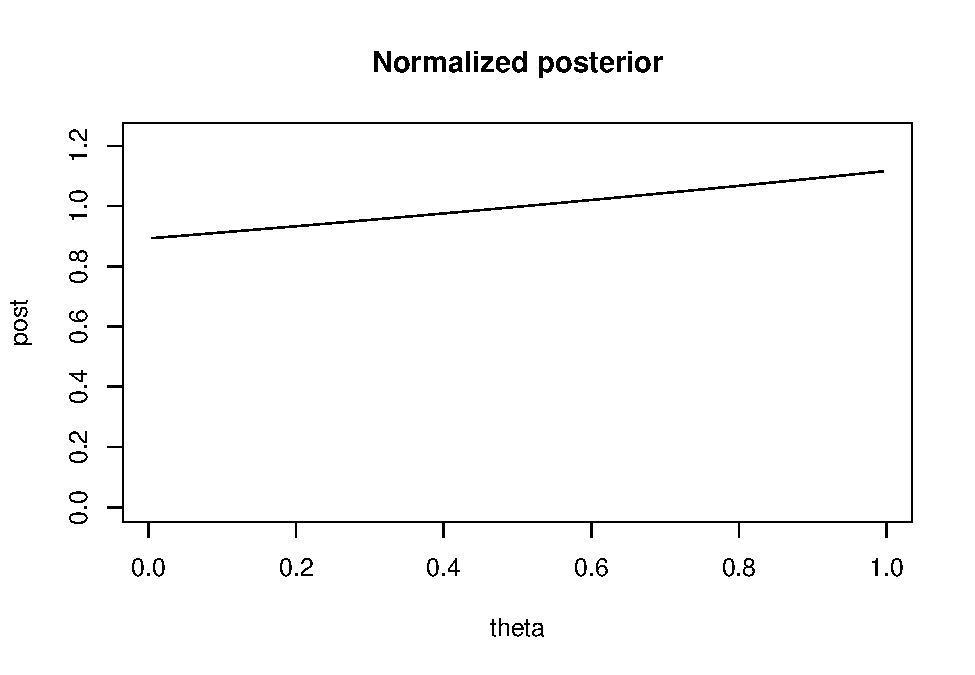
\includegraphics{_main_files/figure-latex/unnamed-chunk-20-1.pdf}

\begin{itemize}
\item
  \begin{enumerate}
  \def\labelenumi{(\alph{enumi})}
  \setcounter{enumi}{1}
  \tightlist
  \item
    Sample 1000 draws from theta from posterior density and plot histogram
    we sample from theta {[}0,100{]} using the grid approximation, and the probability is from the posterior distribution.
  \end{enumerate}
\end{itemize}

\begin{Shaded}
\begin{Highlighting}[]
\NormalTok{  samps}\OtherTok{\textless{}{-}}\NormalTok{(}\FunctionTok{sample}\NormalTok{(theta,}\DecValTok{1000}\NormalTok{,}\AttributeTok{prob=}\NormalTok{post}\SpecialCharTok{*}\NormalTok{step,}\AttributeTok{replace=}\NormalTok{T))}
  \FunctionTok{hist}\NormalTok{(samps,}\AttributeTok{main=}\FunctionTok{mean}\NormalTok{(samps))}
\end{Highlighting}
\end{Shaded}

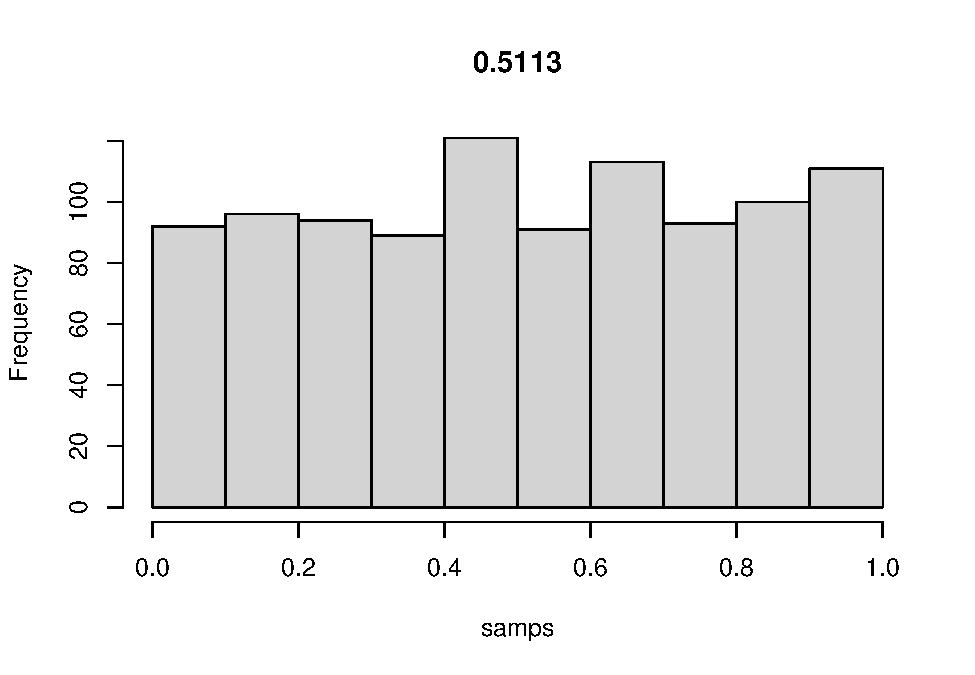
\includegraphics{_main_files/figure-latex/unnamed-chunk-21-1.pdf}

\begin{Shaded}
\begin{Highlighting}[]
  \DocumentationTok{\#\#sample mean is close to the mean of the observed.}
\end{Highlighting}
\end{Shaded}

\begin{itemize}
\item
  \begin{enumerate}
  \def\labelenumi{(\alph{enumi})}
  \setcounter{enumi}{2}
  \tightlist
  \item
    Using the previous 1000 samples of \(\theta\) to obtain 1000 samples from the predictive distribution of a future observation \(y_6\), and plot the predictive draws.
    we use the sampled thetas from the posterior to sample from the Cauchy distribution. The predictive probability follows \(p(x|y) =\int p(x|\theta)p(\theta|y)d\theta\) where \(p(x|\theta)\) follows from the Cauchy distribution, given original sequence of thetas. We have the posterior values for each theta (given the uniform grid of thetas) and take the product. then for each predictive value, we sum the total probability across all thetas to compute the predictive probability. The maximum predictive value probability 0.52 with probability of 0.29.
  \end{enumerate}
\end{itemize}

\begin{Shaded}
\begin{Highlighting}[]
\DocumentationTok{\#\# predictive distribution ? ?? }
 \CommentTok{\# p(x | y) = int p(x|theta)*p(theta|y ) dtheta}
\DocumentationTok{\#\# the posterior is p(theta|y) }
 \CommentTok{\# the likelihood p(x|theta)  \#\# we use the sampled thetas using the posterior}
\NormalTok{ ytilde}\OtherTok{\textless{}{-}}\FunctionTok{rcauchy}\NormalTok{(}\DecValTok{1000}\NormalTok{,}\AttributeTok{location=}\NormalTok{samps,}\AttributeTok{scale=}\DecValTok{1}\NormalTok{) }
 \DocumentationTok{\#\# probability of the samples }
 \CommentTok{\#prob\_samp\textless{}{-}post[match(samps,theta)]}
  \FunctionTok{summary}\NormalTok{(ytilde) }\DocumentationTok{\#\# we have a wide distribution of predictive values.}
\end{Highlighting}
\end{Shaded}

\begin{verbatim}
##      Min.   1st Qu.    Median      Mean   3rd Qu.      Max. 
## -670.5782   -0.5415    0.5497    0.9636    1.6473  718.4207
\end{verbatim}

\begin{Shaded}
\begin{Highlighting}[]
\DocumentationTok{\#\# for all predictive values,  find the total probability  }
   \DocumentationTok{\#\# int p(x|theta)*p(theta|y) d\textbackslash{}theta  note that p(x|theta) is a function of theta, so we input hte theta grid.}
\NormalTok{ pred.prob}\OtherTok{\textless{}{-}}\FunctionTok{sapply}\NormalTok{(ytilde,}\ControlFlowTok{function}\NormalTok{(x) }\FunctionTok{sum}\NormalTok{(}\FunctionTok{dcauchy}\NormalTok{(x,}\AttributeTok{location=}\NormalTok{theta,}\AttributeTok{scale=}\DecValTok{1}\NormalTok{)}\SpecialCharTok{*}\NormalTok{post}\SpecialCharTok{*}\NormalTok{step))  }
  
  \FunctionTok{plot}\NormalTok{(ytilde,pred.prob, }\AttributeTok{main=}\StringTok{\textquotesingle{}predictive distribution\textquotesingle{}}\NormalTok{)}
\end{Highlighting}
\end{Shaded}

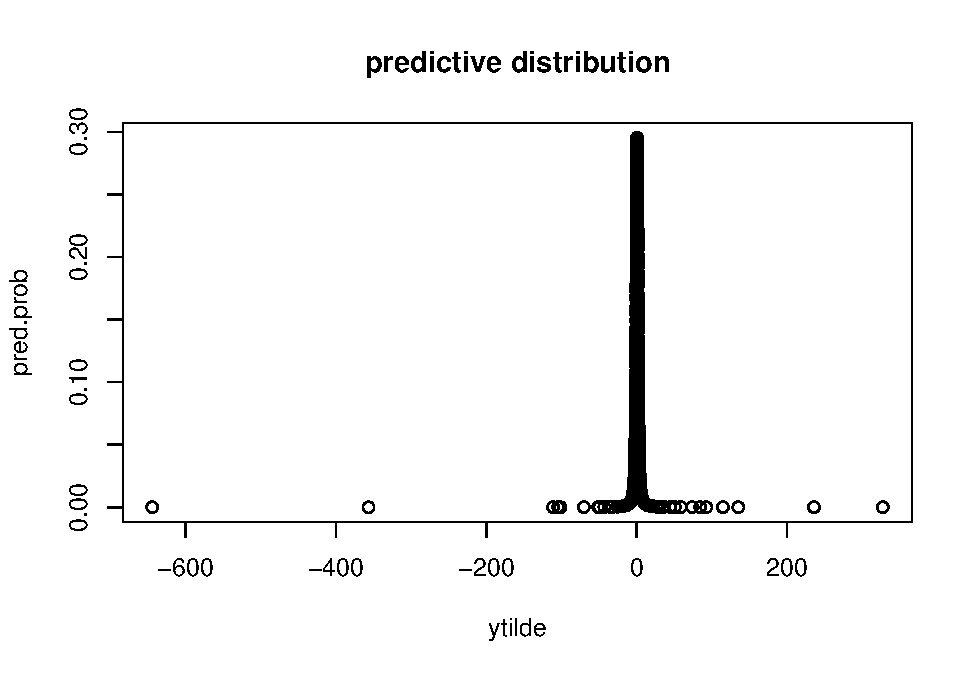
\includegraphics{_main_files/figure-latex/unnamed-chunk-22-1.pdf}

\begin{Shaded}
\begin{Highlighting}[]
  \DocumentationTok{\#\# maximum predictive probability}
  \FunctionTok{message}\NormalTok{(}\StringTok{\textquotesingle{}max pred. prob \textquotesingle{}}\NormalTok{, }\FunctionTok{round}\NormalTok{(ytilde[}\FunctionTok{which}\NormalTok{(pred.prob}\SpecialCharTok{==}\FunctionTok{max}\NormalTok{(pred.prob))],}\DecValTok{3}\NormalTok{))}
\end{Highlighting}
\end{Shaded}

\begin{verbatim}
## max pred. prob 0.525
\end{verbatim}

\hypertarget{question-12}{%
\subsection*{Question 12}\label{question-12}}
\addcontentsline{toc}{subsection}{Question 12}

Suppose \(y|\theta \sim Poisson(\theta)\), find Jeffreys' prior density for \(\theta\) and then find \(\alpha,\beta\) for which Gamma(a,b) density is a close match to Jeffreys' density.

\[
\begin{aligned}
 log(p(y|\theta))&= y*log(\theta)-\theta -log(y!)\\
 &\implies y' = y/\theta - 1 ,  y'' = -y/\theta^2 \\
 &\implies J(\theta)= E(- l'')= E(y/\theta^2)= 1/\theta \\
 &= p(\theta)\propto |J(\theta)^{1/2}| = \sqrt{1/\theta} = \theta^{-1/2}\\
\end{aligned}
\]
So the closes prior is \(\alpha=1/2 , \beta=0\).

\hypertarget{question-13}{%
\subsection*{Question 13}\label{question-13}}
\addcontentsline{toc}{subsection}{Question 13}

\begin{itemize}
\item
  \begin{enumerate}
  \def\labelenumi{(\alph{enumi})}
  \tightlist
  \item
    Use the normal approximation to gamma and poisson to determine a posterior for fatal accidents using table 2.2. Compute the 95\(\%\) predictive interval.
  \end{enumerate}
\item
  We set the empirical prior alpha =25 and beta =1 because the effective sample size (\(\beta\)) is mean is approximately 25, and given these the quantiles of the prior distribution is 16.2 and 35.7 which contains the observed data well. and the prior mean is approximately 25 which is reasonably close to the table 2.2 values, although a sensitivity analysis is recommended.
\item
  We use the conjugate prior for Gamma to find the posterior distribution, which closely is approximated by the normal distribution. The posterior distributions are similar. The normal approximation prior followed \(N(\alpha/\beta, \sqrt{\alpha}/\beta)\). we set the variance to be known \(\sigma^2=100\). Using the gamma conjugate prior the predictive interval is \$95\% \$ (21.1,26.9).
\item
  The posterior predictive value was determined by sample values from the posterior, and using the parameters sampled from posterior to generate a Poisson random variable. The average predictive value is 23.9 fatal accidents.
\end{itemize}

-Using Jeffrey's prior we set alpha=1/2 and beta=0.02 which has a prior mean of 25 which matches the observed mean. The posterior using Jeffreys' prior credible interval 95\(\%\) is (21.11, 26.88) which is similar to the empirical prior. Using the normal approximation to Jeffreys' prior has a 95\(\%\) predictive interval of (14,34) with a predictive mean of 23.83. The posterior predictive value for 1986 was computed by sampling \(\theta\) from the posterior distribution, and for each \(\theta_j\), we sampled a random variable from Poisson(\(\lambda=\theta_j)\).

-Using Jeffreys' prior, the posteror is \(p(\theta|y) \sim Gamma(238.5,10.2)\). Using simulation the \(95\%\) predictive invterval is (14,34). Using the normal approximation
- Using the posterior predictiction equation \(E(x|y) = E(\theta| y) = \mu\). and the V(\(x|y)= E(\theta| y)+ V(\theta | y)\). Using the normal approximation \(\mu_n = 23.8\) and \(\tau_n^2 = 9.9\). Then the posterior variance is 23.8+9.9 = 33.7. Then using \(\mu \pm 1.96\sigma_n = (12.43 35.19)\).
The true observed value for 1986 is 22 fatal accidents.

\begin{Shaded}
\begin{Highlighting}[]
\CommentTok{\# data entry}
\NormalTok{ year}\OtherTok{\textless{}{-}}\FunctionTok{seq}\NormalTok{(}\DecValTok{1976}\NormalTok{,}\DecValTok{1985}\NormalTok{)}
\NormalTok{ fatal}\OtherTok{\textless{}{-}}\FunctionTok{c}\NormalTok{(}\DecValTok{24}\NormalTok{,}\DecValTok{25}\NormalTok{,}\DecValTok{31}\NormalTok{,}\DecValTok{31}\NormalTok{,}\DecValTok{22}\NormalTok{,}\DecValTok{21}\NormalTok{,}\DecValTok{26}\NormalTok{,}\DecValTok{20}\NormalTok{,}\DecValTok{16}\NormalTok{,}\DecValTok{22}\NormalTok{)}
\NormalTok{ death}\OtherTok{\textless{}{-}}\FunctionTok{c}\NormalTok{(}\DecValTok{734}\NormalTok{,}\DecValTok{516}\NormalTok{,}\DecValTok{754}\NormalTok{,}\DecValTok{877}\NormalTok{,}\DecValTok{814}\NormalTok{,}\DecValTok{362}\NormalTok{,}\DecValTok{764}\NormalTok{,}\DecValTok{809}\NormalTok{,}\DecValTok{223}\NormalTok{,}\DecValTok{1066}\NormalTok{)}
\NormalTok{ rate}\OtherTok{\textless{}{-}}\FunctionTok{c}\NormalTok{(}\FloatTok{0.19}\NormalTok{,}\FloatTok{0.12}\NormalTok{,}\FloatTok{0.15}\NormalTok{,}\FloatTok{0.16}\NormalTok{,}\FloatTok{0.14}\NormalTok{,}\FloatTok{0.06}\NormalTok{,}\FloatTok{0.13}\NormalTok{,}\FloatTok{0.13}\NormalTok{,}\FloatTok{0.03}\NormalTok{,}\FloatTok{0.15}\NormalTok{)}
\NormalTok{ data}\OtherTok{\textless{}{-}}\FunctionTok{data.frame}\NormalTok{(}\AttributeTok{year=}\NormalTok{year,}\AttributeTok{fatal=}\NormalTok{fatal,}\AttributeTok{pass.deaths=}\NormalTok{death,}\AttributeTok{death.rate=}\NormalTok{rate)}
 
 \DocumentationTok{\#\# gamma prior on theta\textgreater{}0}
\NormalTok{ theta}\OtherTok{=}\FunctionTok{seq}\NormalTok{(}\AttributeTok{from=}\DecValTok{0}\NormalTok{,}\AttributeTok{to=}\DecValTok{50}\NormalTok{,}\AttributeTok{by=}\NormalTok{.}\DecValTok{01}\NormalTok{)}

 \DocumentationTok{\#\# normal approximation to gamma}
  \DocumentationTok{\#\# Gamma(a,b) ,  mean = a/b,  var = a/b\^{}2  \#\# where beta is the inverse{-}scale}
   \DocumentationTok{\#\# gamma(a,b) \textasciitilde{}  N (a/b, sd= sqrt(a)/b)}
 \DocumentationTok{\#\# normal approx to Pois}
   \DocumentationTok{\#\# Pois(a) ,  mean =a, var= a}
    \DocumentationTok{\#\# Pois(a) \textasciitilde{} N(a,sd= sqrt(a))}
 
 \DocumentationTok{\#\# gamma prior of total count a{-}1,  in b observations }
 \DocumentationTok{\#\# empirical prior}
 \DocumentationTok{\#\# we approximate a prior to have an average of 25 deaths across the decade.  the empirical mean is 23.8 \textasciitilde{} 24}
 \CommentTok{\#  the beta parameter is set rate is set such that gamma(25,1) has quantiles  16.2, 35.7 which matches well the observed data.}
\NormalTok{   alpha}\OtherTok{=} \DecValTok{25}
\NormalTok{   beta}\OtherTok{\textless{}{-}} \DecValTok{1}
   \DocumentationTok{\#\# the mean rate given the data is 0.126, so we find the beta parameter to match the mean rate.}
\NormalTok{   n}\OtherTok{\textless{}{-}}\FunctionTok{nrow}\NormalTok{(data)}
 \FunctionTok{message}\NormalTok{(}\StringTok{"the prior interval:"}\NormalTok{,}\FunctionTok{qgamma}\NormalTok{(}\FunctionTok{c}\NormalTok{(}\FloatTok{0.025}\NormalTok{,}\FloatTok{0.975}\NormalTok{),alpha,beta))}
\end{Highlighting}
\end{Shaded}

\begin{verbatim}
## the prior interval:16.178681847829335.7100975937532
\end{verbatim}

\begin{Shaded}
\begin{Highlighting}[]
\DocumentationTok{\#\# non{-}informative prior using Jeffrey\textquotesingle{}s prior}
\NormalTok{  Jalpha}\OtherTok{=} \DecValTok{1}\SpecialCharTok{/}\DecValTok{2}
\NormalTok{   Jbeta}\OtherTok{\textless{}{-}} \FloatTok{0.02} \DocumentationTok{\#\# we set close to 0}
    \DocumentationTok{\#\# prior mean is 25 which matches the observed data.}
   \DocumentationTok{\#\# the mean rate given the data is 0.126, so we find the beta parameter to match the mean rate.}
\FunctionTok{message}\NormalTok{(}\StringTok{"the prior interval:"}\NormalTok{)}
\end{Highlighting}
\end{Shaded}

\begin{verbatim}
## the prior interval:
\end{verbatim}

\begin{Shaded}
\begin{Highlighting}[]
 \FunctionTok{print}\NormalTok{(}\FunctionTok{qgamma}\NormalTok{(}\FunctionTok{c}\NormalTok{(}\FloatTok{0.025}\NormalTok{,}\FloatTok{0.975}\NormalTok{),Jalpha,Jbeta))}
\end{Highlighting}
\end{Shaded}

\begin{verbatim}
## [1]   0.02455173 125.59715468
\end{verbatim}

\begin{Shaded}
\begin{Highlighting}[]
 \FunctionTok{plot}\NormalTok{(theta,}\FunctionTok{dgamma}\NormalTok{(theta,alpha,}\AttributeTok{rate=}\NormalTok{beta),}\AttributeTok{lty=}\DecValTok{2}\NormalTok{)}
\FunctionTok{lines}\NormalTok{(theta,}\FunctionTok{dgamma}\NormalTok{(theta,alpha}\SpecialCharTok{+}\NormalTok{n}\SpecialCharTok{*}\FunctionTok{mean}\NormalTok{(fatal),}\AttributeTok{rate=}\NormalTok{beta}\SpecialCharTok{+}\NormalTok{n),}\AttributeTok{col=}\StringTok{\textquotesingle{}blue\textquotesingle{}}\NormalTok{)}
\FunctionTok{lines}\NormalTok{(theta,}\FunctionTok{dgamma}\NormalTok{(theta,Jalpha,}\AttributeTok{rate=}\NormalTok{Jbeta),}\AttributeTok{col=}\StringTok{\textquotesingle{}red\textquotesingle{}}\NormalTok{)}
\FunctionTok{lines}\NormalTok{(theta,}\FunctionTok{dgamma}\NormalTok{(theta,Jalpha}\SpecialCharTok{+}\NormalTok{n}\SpecialCharTok{*}\FunctionTok{mean}\NormalTok{(fatal),}\AttributeTok{rate=}\NormalTok{Jbeta}\SpecialCharTok{+}\NormalTok{n),}\AttributeTok{col=}\StringTok{\textquotesingle{}green\textquotesingle{}}\NormalTok{)}
\FunctionTok{legend}\NormalTok{(}\DecValTok{35}\NormalTok{, }\FloatTok{0.06}\NormalTok{, }\AttributeTok{legend=}\FunctionTok{c}\NormalTok{(}\StringTok{"Empr.Prior"}\NormalTok{, }\StringTok{"Posterior1"}\NormalTok{,}\StringTok{"Jeff."}\NormalTok{,}\StringTok{"Posterior2"}\NormalTok{),}
       \AttributeTok{col=}\FunctionTok{c}\NormalTok{(}\StringTok{"black"}\NormalTok{, }\StringTok{"blue"}\NormalTok{,}\StringTok{"red"}\NormalTok{,}\StringTok{"green"}\NormalTok{), }\AttributeTok{lty=}\DecValTok{1}\NormalTok{, }\AttributeTok{cex=}\FloatTok{0.8}\NormalTok{)}
\end{Highlighting}
\end{Shaded}

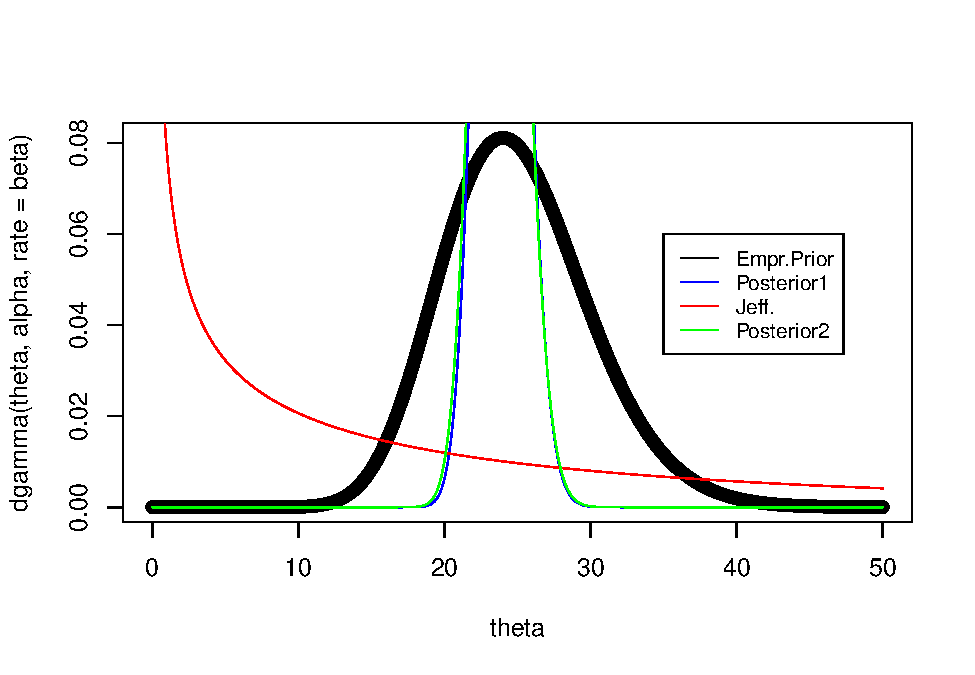
\includegraphics{_main_files/figure-latex/unnamed-chunk-23-1.pdf}

\begin{Shaded}
\begin{Highlighting}[]
 \DocumentationTok{\#\# credible interval of the posterior}
\NormalTok{ pois\_credible}\OtherTok{\textless{}{-}}\FunctionTok{qgamma}\NormalTok{(}\FunctionTok{c}\NormalTok{(.}\DecValTok{025}\NormalTok{,}\FloatTok{0.975}\NormalTok{),alpha}\SpecialCharTok{+}\NormalTok{n}\SpecialCharTok{*}\FunctionTok{mean}\NormalTok{(fatal),}\AttributeTok{rate=}\NormalTok{beta}\SpecialCharTok{+}\NormalTok{n)}
 \FunctionTok{message}\NormalTok{(}\StringTok{"posterior gamma interval n=10: "}\NormalTok{,pois\_credible[}\DecValTok{1}\NormalTok{],}\StringTok{" "}\NormalTok{,pois\_credible[}\DecValTok{2}\NormalTok{]) }\DocumentationTok{\#\# }
\end{Highlighting}
\end{Shaded}

\begin{verbatim}
## posterior gamma interval n=10: 21.1065649790459 26.883779321636
\end{verbatim}

\begin{Shaded}
\begin{Highlighting}[]
 \DocumentationTok{\#\# jeffrey\textquotesingle{}s prior}
\NormalTok{  pois\_credible\_jp}\OtherTok{\textless{}{-}}\FunctionTok{qgamma}\NormalTok{(}\FunctionTok{c}\NormalTok{(.}\DecValTok{025}\NormalTok{,}\FloatTok{0.975}\NormalTok{),Jalpha}\SpecialCharTok{+}\NormalTok{n}\SpecialCharTok{*}\FunctionTok{mean}\NormalTok{(fatal),}\AttributeTok{rate=}\NormalTok{Jbeta}\SpecialCharTok{+}\NormalTok{n)}
 \FunctionTok{message}\NormalTok{(}\StringTok{"posterior gamma interval n=10: "}\NormalTok{,pois\_credible[}\DecValTok{1}\NormalTok{],}\StringTok{" "}\NormalTok{,pois\_credible[}\DecValTok{2}\NormalTok{]) }\DocumentationTok{\#\# }
\end{Highlighting}
\end{Shaded}

\begin{verbatim}
## posterior gamma interval n=10: 21.1065649790459 26.883779321636
\end{verbatim}

\begin{Shaded}
\begin{Highlighting}[]
\NormalTok{ post\_pois}\OtherTok{\textless{}{-}}\FunctionTok{dgamma}\NormalTok{(theta,Jalpha}\SpecialCharTok{+}\NormalTok{n}\SpecialCharTok{*}\FunctionTok{mean}\NormalTok{(fatal),}\AttributeTok{rate=}\NormalTok{Jbeta}\SpecialCharTok{+}\NormalTok{n)}
  \DocumentationTok{\#\# posterior mean is 23.8}
 \FunctionTok{sum}\NormalTok{(theta}\SpecialCharTok{*}\NormalTok{post\_pois}\SpecialCharTok{/}\FunctionTok{sum}\NormalTok{(post\_pois))}
\end{Highlighting}
\end{Shaded}

\begin{verbatim}
## [1] 23.8024
\end{verbatim}

\begin{Shaded}
\begin{Highlighting}[]
 \CommentTok{\# normal approximation using Jeffrey\textquotesingle{}s Prior}
\NormalTok{  mu\_0}\OtherTok{\textless{}{-}}\NormalTok{ Jalpha}\SpecialCharTok{/}\NormalTok{Jbeta  }\DocumentationTok{\#\# average of 12.6 fatal accidents}
\NormalTok{  tau2\_0}\OtherTok{\textless{}{-}}\NormalTok{ Jalpha}\SpecialCharTok{/}\NormalTok{Jbeta}\SpecialCharTok{\^{}}\DecValTok{2} \DocumentationTok{\#\# }
  
\NormalTok{  sigma2}\OtherTok{\textless{}{-}}\DecValTok{10}\SpecialCharTok{\^{}}\DecValTok{2}  \DocumentationTok{\#\# we assume we know the variance of the fatalities (empirical variance is 22.2) so we set it to 50 (large enough)}
  
  
\NormalTok{  mu\_n}\OtherTok{\textless{}{-}}\ControlFlowTok{function}\NormalTok{(mu0,ybar,n,tau02,sigma2)\{}
\NormalTok{  mun}\OtherTok{\textless{}{-}}\NormalTok{ (mu0}\SpecialCharTok{/}\NormalTok{tau02 }\SpecialCharTok{+}\NormalTok{ (ybar}\SpecialCharTok{*}\NormalTok{n)}\SpecialCharTok{/}\NormalTok{sigma2)}\SpecialCharTok{/}\NormalTok{(}\DecValTok{1}\SpecialCharTok{/}\NormalTok{tau02 }\SpecialCharTok{+}\NormalTok{ n}\SpecialCharTok{/}\NormalTok{sigma2)}
  \FunctionTok{return}\NormalTok{(mun)}
\NormalTok{\}}
\NormalTok{taun2}\OtherTok{\textless{}{-}}\ControlFlowTok{function}\NormalTok{(tau02,n,sigma2)\{}
\NormalTok{  inv.taun2}\OtherTok{\textless{}{-}} \DecValTok{1}\SpecialCharTok{/}\NormalTok{tau02 }\SpecialCharTok{+}\NormalTok{n}\SpecialCharTok{/}\NormalTok{sigma2}
  \FunctionTok{return}\NormalTok{(}\DecValTok{1}\SpecialCharTok{/}\NormalTok{inv.taun2)}
\NormalTok{\}}

\NormalTok{ybar}\OtherTok{=}\FunctionTok{mean}\NormalTok{(fatal)}

\NormalTok{ mn}\OtherTok{\textless{}{-}}\FunctionTok{mu\_n}\NormalTok{(mu\_0,ybar,tau2\_0,n,sigma2)}
\NormalTok{ tn}\OtherTok{\textless{}{-}}\FunctionTok{taun2}\NormalTok{(tau2\_0,n,sigma2)}
\DocumentationTok{\#\# posterior interval n=10}
  \CommentTok{\#lower\textless{}{-}round(qnorm(0.025,mu\_n(mu0,ybar,tau02,10,sigma2),sd=sqrt(taun2(tau02,10,sigma2))),2)}
  \FunctionTok{print}\NormalTok{(}\FunctionTok{c}\NormalTok{(mn}\FloatTok{{-}1.96}\SpecialCharTok{*}\FunctionTok{sqrt}\NormalTok{(mn}\SpecialCharTok{+}\NormalTok{tn), mn}\FloatTok{+1.96}\SpecialCharTok{*}\FunctionTok{sqrt}\NormalTok{(mn}\SpecialCharTok{+}\NormalTok{tn)))}
\end{Highlighting}
\end{Shaded}

\begin{verbatim}
## [1] 12.42630 35.19275
\end{verbatim}

\begin{Shaded}
\begin{Highlighting}[]
\DocumentationTok{\#\# posterior predictive value}
   \DocumentationTok{\#\# check this with the grid approach in the Gamma framework.  }
\NormalTok{  theta\_samps}\OtherTok{\textless{}{-}}\FunctionTok{sample}\NormalTok{(theta,}\DecValTok{10000}\NormalTok{,}\AttributeTok{prob=}\NormalTok{post\_pois,}\AttributeTok{replace=}\NormalTok{T)}
\NormalTok{   ytilde}\OtherTok{\textless{}{-}}\FunctionTok{rpois}\NormalTok{(}\DecValTok{10000}\NormalTok{,}\AttributeTok{lambda=}\NormalTok{theta\_samps) }
 \DocumentationTok{\#\# probability of the samples }
 \CommentTok{\#prob\_samp\textless{}{-}post[match(samps,theta)]}
  \FunctionTok{summary}\NormalTok{(ytilde) }\DocumentationTok{\#\# we have a wide distribution of predictive values.}
\end{Highlighting}
\end{Shaded}

\begin{verbatim}
##    Min. 1st Qu.  Median    Mean 3rd Qu.    Max. 
##    8.00   20.00   24.00   23.87   27.00   48.00
\end{verbatim}

\begin{Shaded}
\begin{Highlighting}[]
\DocumentationTok{\#\# for all predictive values,  find the total probability  }
   \DocumentationTok{\#\# int p(x|theta)*p(theta|y) d\textbackslash{}theta  note that p(x|theta) is a function of theta, so we input hte theta grid.}
\NormalTok{ pred.prob}\OtherTok{\textless{}{-}}\FunctionTok{sapply}\NormalTok{(ytilde,}\ControlFlowTok{function}\NormalTok{(x) }\FunctionTok{sum}\NormalTok{(}\FunctionTok{dpois}\NormalTok{(x,}\AttributeTok{lambda =}\NormalTok{ theta)}\SpecialCharTok{*}\NormalTok{post\_pois}\SpecialCharTok{/}\FunctionTok{sum}\NormalTok{(post\_pois)))  }
  
 \FunctionTok{plot}\NormalTok{(ytilde,pred.prob, }\AttributeTok{main=}\StringTok{\textquotesingle{}predictive distribution for future 1986\textquotesingle{}}\NormalTok{)}
 \FunctionTok{abline}\NormalTok{(}\AttributeTok{v=}\FunctionTok{quantile}\NormalTok{(ytilde,}\FunctionTok{c}\NormalTok{(}\FloatTok{0.025}\NormalTok{,}\FloatTok{0.975}\NormalTok{)),}\AttributeTok{col=}\StringTok{\textquotesingle{}red\textquotesingle{}}\NormalTok{)}
\end{Highlighting}
\end{Shaded}

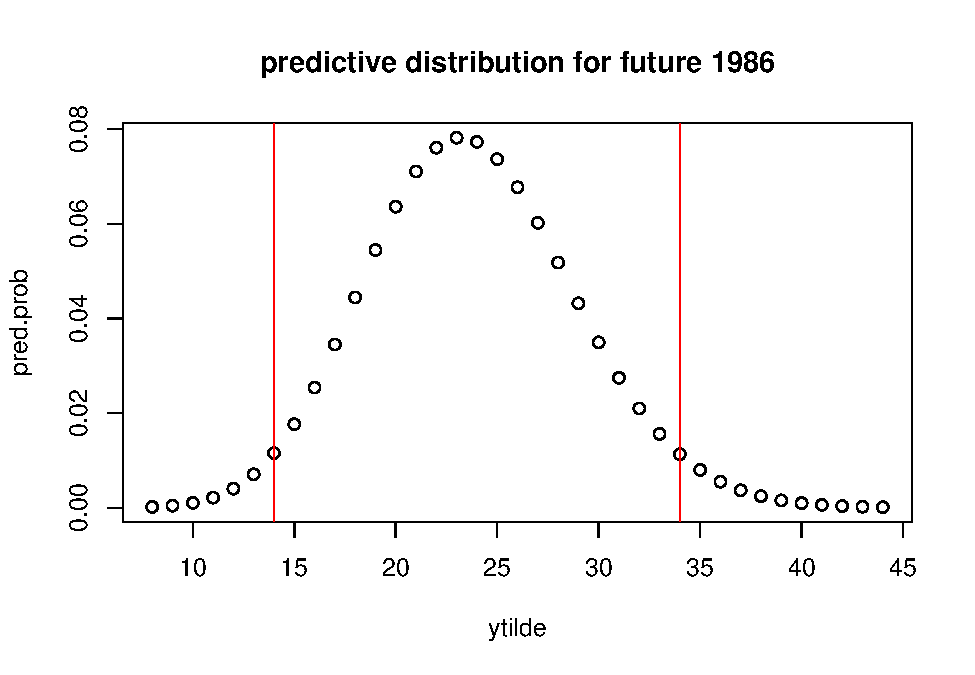
\includegraphics{_main_files/figure-latex/unnamed-chunk-23-2.pdf}

\begin{Shaded}
\begin{Highlighting}[]
 \CommentTok{\#lines(theta,post\_pois)}
 \FunctionTok{quantile}\NormalTok{(ytilde,}\FunctionTok{c}\NormalTok{(}\FloatTok{0.025}\NormalTok{,}\FloatTok{0.975}\NormalTok{))}
\end{Highlighting}
\end{Shaded}

\begin{verbatim}
##  2.5% 97.5% 
##    15    35
\end{verbatim}

From the gamma posterior \(E(\theta | y) = 238.5/10.02=24.25\) and the variance \(V(\theta|y)= 238.5/10.02^2=2.87\). From the Poisson likelihood \(E(x|\theta)=\theta\) and \(V(x|\theta)=\theta\). \(V(x|y)= E(V(x|\theta,y) | y) + V(E(x|\theta,y)|y)= E(\theta| y)+ V(\theta|y) = 23.382+2.87= 26.252\)

Using the normal approximation on the posterior values, the variance of the predictive value and is a larger interval (14.21, 34.3).

The average predictive value from 1986 is 24.3 which is close to the true value 22 fatal accidents.

\begin{Shaded}
\begin{Highlighting}[]
  \DocumentationTok{\#\# Predictive with normal}

\DocumentationTok{\#\# using the normal approximation}
\DocumentationTok{\#\# predictive interval must use a grid approach.}
\NormalTok{     pred}\OtherTok{\textless{}{-}}\FunctionTok{round}\NormalTok{(}\FunctionTok{qnorm}\NormalTok{(}\FunctionTok{c}\NormalTok{(}\FloatTok{0.025}\NormalTok{,}\FloatTok{0.975}\NormalTok{),}\FloatTok{24.25}\NormalTok{,}\AttributeTok{sd=}\FunctionTok{sqrt}\NormalTok{(}\FloatTok{26.252}\NormalTok{)),}\DecValTok{2}\NormalTok{)}
  \FunctionTok{message}\NormalTok{(}\StringTok{"predictive interval n=10: "}\NormalTok{,pred[}\DecValTok{1}\NormalTok{],}\StringTok{" "}\NormalTok{,pred[}\DecValTok{2}\NormalTok{])}
\end{Highlighting}
\end{Shaded}

\begin{verbatim}
## predictive interval n=10: 14.21 34.29
\end{verbatim}

\begin{Shaded}
\begin{Highlighting}[]
   \DocumentationTok{\#\# check this with the grid approach in the normal framework.  }
\NormalTok{  post\_pred\_norm}\OtherTok{\textless{}{-}}\NormalTok{(}\FunctionTok{dnorm}\NormalTok{(theta,}\FloatTok{24.25}\NormalTok{,}\FunctionTok{sqrt}\NormalTok{(}\FloatTok{26.252}\NormalTok{))}\SpecialCharTok{/}\FunctionTok{sum}\NormalTok{(}\FunctionTok{dnorm}\NormalTok{(theta,}\FloatTok{24.25}\NormalTok{,}\FunctionTok{sqrt}\NormalTok{(}\FloatTok{26.252}\NormalTok{))))}
\NormalTok{   ytilde\_norm}\OtherTok{\textless{}{-}}\FunctionTok{rnorm}\NormalTok{(}\DecValTok{100000}\NormalTok{,}\AttributeTok{mean=}\FloatTok{24.25}\NormalTok{,}\AttributeTok{sd=}\FunctionTok{sqrt}\NormalTok{(}\FloatTok{26.252}\NormalTok{)) }
 \DocumentationTok{\#\# probability of the samples }
 \CommentTok{\#prob\_samp\textless{}{-}post[match(samps,theta)]}
  \FunctionTok{summary}\NormalTok{(ytilde\_norm) }\DocumentationTok{\#\# we have a wide distribution of predictive values.}
\end{Highlighting}
\end{Shaded}

\begin{verbatim}
##    Min. 1st Qu.  Median    Mean 3rd Qu.    Max. 
##   2.484  20.820  24.235  24.241  27.694  46.730
\end{verbatim}

\begin{Shaded}
\begin{Highlighting}[]
\DocumentationTok{\#\# for all predictive values,  find the total probability  }
   \DocumentationTok{\#\# int p(x|theta)*p(theta|y) d\textbackslash{}theta  note that p(x|theta) is a function of theta, so we input hte theta grid.}
\NormalTok{ pred.prob\_norm}\OtherTok{\textless{}{-}}\FunctionTok{sapply}\NormalTok{(ytilde\_norm,}\ControlFlowTok{function}\NormalTok{(x) }\FunctionTok{sum}\NormalTok{(}\FunctionTok{dnorm}\NormalTok{(x,}\FloatTok{24.25}\NormalTok{,}\FunctionTok{sqrt}\NormalTok{(}\FloatTok{26.252}\NormalTok{))}\SpecialCharTok{*}\NormalTok{post\_pred\_norm))  }
  
 \FunctionTok{plot}\NormalTok{(ytilde\_norm,pred.prob\_norm, }\AttributeTok{main=}\StringTok{\textquotesingle{}predictive distribution for future 1986\textquotesingle{}}\NormalTok{)}
 \FunctionTok{abline}\NormalTok{(}\AttributeTok{v=}\FunctionTok{quantile}\NormalTok{(ytilde\_norm,}\FunctionTok{c}\NormalTok{(}\FloatTok{0.025}\NormalTok{,}\FloatTok{0.975}\NormalTok{)),}\AttributeTok{col=}\StringTok{\textquotesingle{}red\textquotesingle{}}\NormalTok{)}
 \FunctionTok{lines}\NormalTok{(theta,post\_pred\_norm)}
\end{Highlighting}
\end{Shaded}

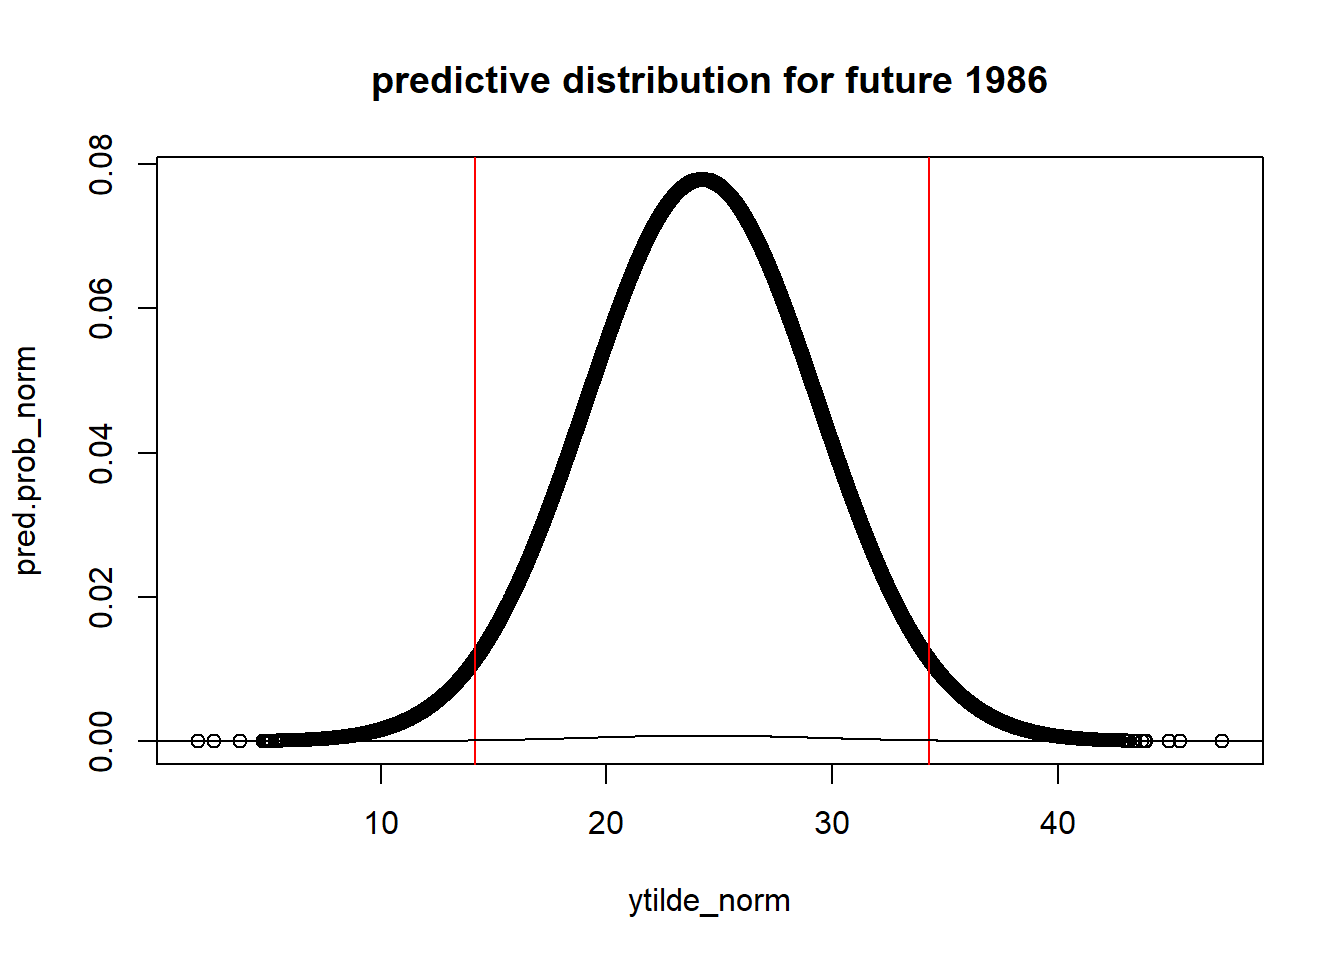
\includegraphics{_main_files/figure-latex/unnamed-chunk-24-1.pdf}

\begin{Shaded}
\begin{Highlighting}[]
 \FunctionTok{quantile}\NormalTok{(ytilde\_norm,}\FunctionTok{c}\NormalTok{(}\FloatTok{0.025}\NormalTok{,}\FloatTok{0.975}\NormalTok{))}
\end{Highlighting}
\end{Shaded}

\begin{verbatim}
##     2.5%    97.5% 
## 14.18024 34.30159
\end{verbatim}

\begin{Shaded}
\begin{Highlighting}[]
 \FunctionTok{message}\NormalTok{(}\StringTok{"average predictive value from posterior:"}\NormalTok{, }\FunctionTok{mean}\NormalTok{(ytilde))}
\end{Highlighting}
\end{Shaded}

\begin{verbatim}
## average predictive value from posterior:23.8698
\end{verbatim}

\begin{itemize}
\item
  \begin{enumerate}
  \def\labelenumi{(\alph{enumi})}
  \setcounter{enumi}{1}
  \tightlist
  \item
    Assume fatal accidents follow a Poisson distribution with a constant rate and an exposure in each year proportional to the number of passanger miles flown. Set a prior and determine a posterior and predictive distribution. estimate the number of passanger miles flown in each year by dividing
  \end{enumerate}
\end{itemize}

let \(\theta\) be the fatal accidents \emph{rate} per 100,000 million miles flown. and let \(x_i\) be the number per 100,000 million miles flown. We compute the miles by dividing the passenger deaths divided by the death rate (deaths per 100,000 million miles flown).

We then compute the fatal accident rate by computing the (passanger deaths per 100,000 million miles)*(number of fatal accidents / number of passenger deaths). We let \(\theta\) = fatal accidents per 100 million miles flown.

The mean accident rate is 0.004, so we set alpha =5 and beta = 1000, so the prior mean is 0.005 (95\(\%\): 0.002,0.01) which is similar to the observed ranges. This is using the observed data to create an empirically driven prior.

However, we must use the Jeffreys' prior for a non-informative prior setting \(\alpha=0.01, \beta=0.01\).

Using Jeffreys' prior, the posterior is Gamma(238.01, 5.716e12) with a 95 credible interval of (3.65e-11, 4.71e-11).

Now for the posterior predictive value, because the parameters space is so small, we sample \(\theta\) from \(p(\theta | y)\) Gamma posterior to generate \(\theta\). In the previous exercise, we used theta from a uniform sequence, but these values are so small due to the scaling it is easier to sample directly from the posterior using \texttt{rgamma}. THen we find the predictive value \(x \sim Pois(8e11*\theta_j)\) by random sampling observation variables from the posterior, and sorting them for the 95 predictive interval.

We can also use the normal approximation, but the equations for the mean and variance must be scaled by the factor 8e11.

\begin{Shaded}
\begin{Highlighting}[]
\NormalTok{ miles100}\OtherTok{\textless{}{-}}\NormalTok{death}\SpecialCharTok{/}\NormalTok{rate }\DocumentationTok{\#\# 100 million miles}
\NormalTok{miles }\OtherTok{=}\NormalTok{ miles100}\SpecialCharTok{*}\FloatTok{1e+08}


  
\DocumentationTok{\#\# likelihood   }
\DocumentationTok{\#\# y | miles, theta \textasciitilde{} Pois( miles*theta)}
  
\NormalTok{ theta}\OtherTok{=}\FunctionTok{seq}\NormalTok{(}\AttributeTok{from=}\DecValTok{0}\NormalTok{,}\AttributeTok{to=}\FloatTok{0.1}\NormalTok{,}\AttributeTok{by=}\NormalTok{.}\DecValTok{001}\NormalTok{)}
 \DocumentationTok{\#\# empirical prior}
\NormalTok{  alpha}\OtherTok{=} \DecValTok{5}
\NormalTok{   beta}\OtherTok{\textless{}{-}} \DecValTok{1000}  
   \DocumentationTok{\#\# the mean is 0.005 and quantiles 0.002 and 0.01 which is close to the observed rates }
   \CommentTok{\#mean(acc\_rate) \#\# fatal accidents per 100,000 million miles driven}
   \FunctionTok{print}\NormalTok{(}\StringTok{"empirical prior 95\% quantiles: "}\NormalTok{)}
\end{Highlighting}
\end{Shaded}

\begin{verbatim}
## [1] "empirical prior 95% quantiles: "
\end{verbatim}

\begin{Shaded}
\begin{Highlighting}[]
   \FunctionTok{qgamma}\NormalTok{(}\FunctionTok{c}\NormalTok{(}\FloatTok{0.025}\NormalTok{,}\FloatTok{0.975}\NormalTok{),alpha,}\AttributeTok{rate=}\NormalTok{beta)}
\end{Highlighting}
\end{Shaded}

\begin{verbatim}
## [1] 0.001623486 0.010241589
\end{verbatim}

\begin{Shaded}
\begin{Highlighting}[]
   \DocumentationTok{\#\# the mean rate given the data is 0.126, so we find the beta parameter to match the mean rate.}
\NormalTok{   n}\OtherTok{\textless{}{-}}\FunctionTok{nrow}\NormalTok{(data)}
   
\DocumentationTok{\#\# we must use Jeffreys\textquotesingle{} prior!!     }
\NormalTok{  Jalpha}\OtherTok{=}\FloatTok{0.01}
\NormalTok{  Jbeta}\OtherTok{\textless{}{-}}\FloatTok{0.01}
 \FunctionTok{plot}\NormalTok{(theta,}\FunctionTok{dgamma}\NormalTok{(theta,Jalpha,}\AttributeTok{rate=}\NormalTok{Jbeta),}\AttributeTok{col=}\StringTok{\textquotesingle{}blue\textquotesingle{}}\NormalTok{)}
\FunctionTok{lines}\NormalTok{(theta,}\FunctionTok{dgamma}\NormalTok{(theta,Jalpha}\SpecialCharTok{+}\FunctionTok{sum}\NormalTok{(fatal),}\AttributeTok{rate=}\NormalTok{Jbeta}\SpecialCharTok{+}\FunctionTok{sum}\NormalTok{(miles)),}\AttributeTok{col=}\StringTok{\textquotesingle{}red\textquotesingle{}}\NormalTok{)}
\end{Highlighting}
\end{Shaded}

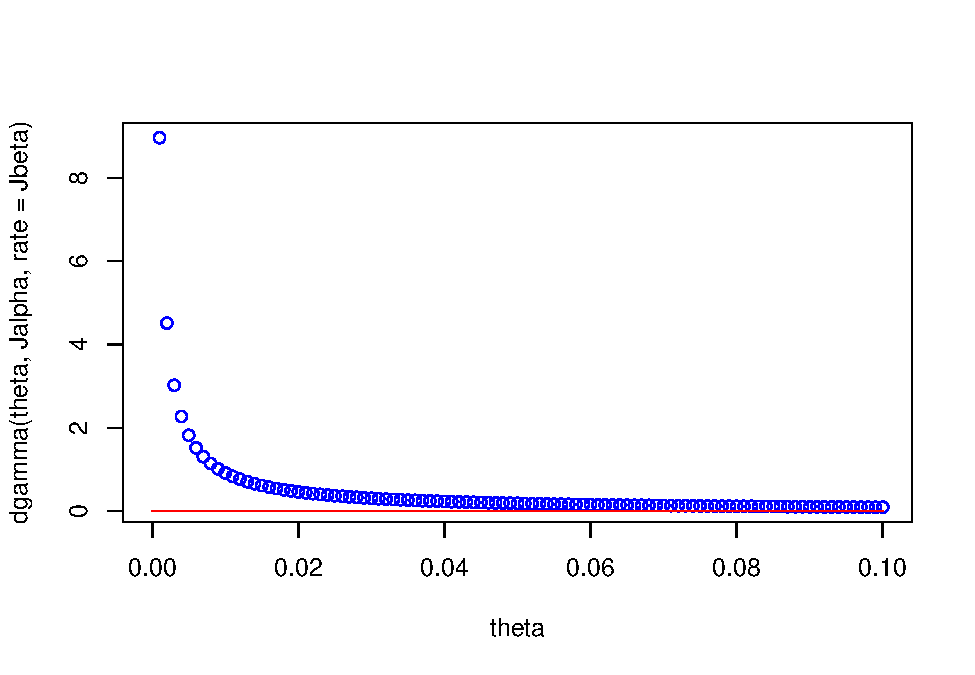
\includegraphics{_main_files/figure-latex/unnamed-chunk-25-1.pdf}

\begin{Shaded}
\begin{Highlighting}[]
 \DocumentationTok{\#\# credible interval of the posterior}
\NormalTok{ pois\_credible}\OtherTok{\textless{}{-}}\FunctionTok{qgamma}\NormalTok{(}\FunctionTok{c}\NormalTok{(.}\DecValTok{025}\NormalTok{,}\FloatTok{0.975}\NormalTok{),Jalpha}\SpecialCharTok{+}\FunctionTok{sum}\NormalTok{(fatal),}\AttributeTok{rate=}\NormalTok{Jbeta}\SpecialCharTok{+}\FunctionTok{sum}\NormalTok{(miles))}
 \FunctionTok{message}\NormalTok{(}\StringTok{"Jeffreys\textquotesingle{} prior posterior gamma interval n=10: "}\NormalTok{)}
\end{Highlighting}
\end{Shaded}

\begin{verbatim}
## Jeffreys' prior posterior gamma interval n=10:
\end{verbatim}

\begin{Shaded}
\begin{Highlighting}[]
 \FunctionTok{print}\NormalTok{(pois\_credible) }\DocumentationTok{\#\# }
\end{Highlighting}
\end{Shaded}

\begin{verbatim}
## [1] 3.651772e-11 4.709401e-11
\end{verbatim}

\begin{Shaded}
\begin{Highlighting}[]
 \DocumentationTok{\#\# generate parameters from the posterior we sample thetas.}
\NormalTok{  theta\_post}\OtherTok{\textless{}{-}}\FunctionTok{rgamma}\NormalTok{(}\DecValTok{1000}\NormalTok{,Jalpha}\SpecialCharTok{+}\FunctionTok{sum}\NormalTok{(fatal),}\AttributeTok{rate=}\NormalTok{Jbeta}\SpecialCharTok{+}\FunctionTok{sum}\NormalTok{(miles))}
\NormalTok{  y1986}\OtherTok{\textless{}{-}}\FunctionTok{rpois}\NormalTok{(}\DecValTok{1000}\NormalTok{,}\FloatTok{8e+11}\SpecialCharTok{*}\NormalTok{theta\_post) }\DocumentationTok{\#\# use in the likelihood}
 \CommentTok{\# message(" predictive 1986 interval: ")}
 \CommentTok{\# sort(y1986)[c(25,976)]}
  
  
\DocumentationTok{\#\#\# the original sequenced theta do not produce parameters from the posterior and this fails.  }
  \CommentTok{\# post\_pois\textless{}{-}dgamma(theta,Jalpha+sum(fatal),rate=Jbeta+sum(miles))}
 \CommentTok{\# theta\_samps\textless{}{-}sample(theta,100000,prob=post\_pois,replace=T)}
  \CommentTok{\# ytilde\textless{}{-}rpois(100000,lambda=8e+11*theta\_samps) }
  
  
\NormalTok{  post\_a}\OtherTok{=}\NormalTok{ Jalpha}\SpecialCharTok{+}\FunctionTok{sum}\NormalTok{(fatal)}
\NormalTok{  post\_b}\OtherTok{=}\NormalTok{ Jbeta}\SpecialCharTok{+}\FunctionTok{sum}\NormalTok{(miles)}
   \DocumentationTok{\#\# use the normal approximation}
   \DocumentationTok{\#\# E = a/b  V = a/b\^{}2}
\NormalTok{   mn\_a }\OtherTok{=}\NormalTok{ post\_a}\SpecialCharTok{/}\NormalTok{post\_b}
\NormalTok{   tn\_a }\OtherTok{=}\NormalTok{ post\_a}\SpecialCharTok{/}\NormalTok{post\_b}\SpecialCharTok{\^{}}\DecValTok{2}
   \DocumentationTok{\#\# xi*E(\textbackslash{}theta | y) = xi*mu\_1}
\NormalTok{   mu\_approx }\OtherTok{=}\NormalTok{ mn\_a}\SpecialCharTok{*}\FloatTok{8e+11}
   \DocumentationTok{\#\# V(x|y) = xi*E(\textbackslash{}theta|y) + xi\^{}2*V(\textbackslash{}theta|y) using the poisson likelihood and xi is the constant.}
\NormalTok{   sigma2\_approx}\OtherTok{\textless{}{-}}\NormalTok{mn\_a}\SpecialCharTok{*}\FloatTok{8e+11}\SpecialCharTok{+}\NormalTok{(}\FloatTok{8e+11}\NormalTok{)}\SpecialCharTok{\^{}}\DecValTok{2}\SpecialCharTok{*}\NormalTok{tn\_a}

   \DocumentationTok{\#\# normal approxim}
\NormalTok{ upper}\OtherTok{\textless{}{-}}\NormalTok{ mu\_approx}\FloatTok{+1.96}\SpecialCharTok{*}\FunctionTok{sqrt}\NormalTok{(sigma2\_approx) }\DocumentationTok{\#\# 46}
\NormalTok{ lower}\OtherTok{\textless{}{-}}\NormalTok{ mu\_approx}\FloatTok{{-}1.96}\SpecialCharTok{*}\FunctionTok{sqrt}\NormalTok{(sigma2\_approx) }\DocumentationTok{\#\# 22}
 \FunctionTok{message}\NormalTok{(}\StringTok{"normal approx: 95\% pred. interval "}\NormalTok{)}
\end{Highlighting}
\end{Shaded}

\begin{verbatim}
## normal approx: 95% pred. interval
\end{verbatim}

\begin{Shaded}
\begin{Highlighting}[]
 \FunctionTok{print}\NormalTok{(}\FunctionTok{c}\NormalTok{(lower,upper))}
\end{Highlighting}
\end{Shaded}

\begin{verbatim}
## [1] 21.23396 45.39038
\end{verbatim}

\begin{Shaded}
\begin{Highlighting}[]
 \FunctionTok{message}\NormalTok{(}\StringTok{" 8,000 per 100 million miles flown has fatality rate: Gamma posterior"}\NormalTok{)}
\end{Highlighting}
\end{Shaded}

\begin{verbatim}
##  8,000 per 100 million miles flown has fatality rate: Gamma posterior
\end{verbatim}

\begin{Shaded}
\begin{Highlighting}[]
 \FunctionTok{print}\NormalTok{(}\FunctionTok{sort}\NormalTok{(y1986)[}\FunctionTok{c}\NormalTok{(}\DecValTok{25}\NormalTok{,}\DecValTok{976}\NormalTok{)])}
\end{Highlighting}
\end{Shaded}

\begin{verbatim}
## [1] 21 46
\end{verbatim}

\begin{Shaded}
\begin{Highlighting}[]
 \FunctionTok{message}\NormalTok{(}\StringTok{" 8,000 per 100 million miles flown has fatality rate: normal approx"}\NormalTok{)}
\end{Highlighting}
\end{Shaded}

\begin{verbatim}
##  8,000 per 100 million miles flown has fatality rate: normal approx
\end{verbatim}

\begin{Shaded}
\begin{Highlighting}[]
 \FunctionTok{print}\NormalTok{(}\FunctionTok{c}\NormalTok{(lower,upper))}
\end{Highlighting}
\end{Shaded}

\begin{verbatim}
## [1] 21.23396 45.39038
\end{verbatim}

\begin{itemize}
\item
  \begin{enumerate}
  \def\labelenumi{(\alph{enumi})}
  \setcounter{enumi}{2}
  \tightlist
  \item
    we repeat part (a) but for passenger deaths. we need to find a prior and determine the posterior distribution with a predictive interval.
  \end{enumerate}
\end{itemize}

We used an empirically derived prior, which does not match the solution, and so we include Jeffreys' prior setting \(\alpha=1/2, \beta=0.01\).

Note that the death rate mean is not equal to the variance so the performance is not as good compared to the fatal accidents.

The 1986 prediction mean is 692 \(95\%\) (638, 750) using the empirical derived priors estimated from the data.\\
If we use Jeffreys' prior the prediction interval is (638,741.05).

which is not the expected prediction of 546 passenger deaths. This is likely because Poisson is not a good fit because it is constrained.

\begin{Shaded}
\begin{Highlighting}[]
\NormalTok{ theta}\OtherTok{=}\FunctionTok{seq}\NormalTok{(}\AttributeTok{from=}\DecValTok{200}\NormalTok{,}\AttributeTok{to=}\DecValTok{1500}\NormalTok{,}\AttributeTok{by=}\NormalTok{.}\DecValTok{1}\NormalTok{)}

 \DocumentationTok{\#\# normal approximation to gamma}
  \DocumentationTok{\#\# Gamma(a,b) ,  mean = a/b,  var = a/b\^{}2  \#\# where beta is the inverse{-}scale}
   \DocumentationTok{\#\# gamma(a,b) \textasciitilde{}  N (a/b, sd= sqrt(a)/b)}
 \DocumentationTok{\#\# normal approx to Pois}
   \DocumentationTok{\#\# Pois(a) ,  mean =a, var= a}
    \DocumentationTok{\#\# Pois(a) \textasciitilde{} N(a,sd= sqrt(a))}
 
 \DocumentationTok{\#\# gamma prior of total count a{-}1,  in b observations }
 \DocumentationTok{\#\# }
 \DocumentationTok{\#\# we approximate a prior to have an average of 600 passenger deaths across the decade.  }
\CommentTok{\#the empirical mean is 691 and variance is  63700.32}
\CommentTok{\# a/b =  691  and a/b\^{}2 = 63700.32,  we solve for a and b}
 \CommentTok{\#  the beta parameter is set rate is set such that   404, 832 which matches well the observed data.}
\NormalTok{   alpha}\OtherTok{=} \DecValTok{8}
\NormalTok{   beta}\OtherTok{\textless{}{-}} \FloatTok{0.0108618}
   \DocumentationTok{\#\# the pr}
\NormalTok{   n}\OtherTok{\textless{}{-}}\FunctionTok{nrow}\NormalTok{(data)}
 \FunctionTok{message}\NormalTok{(}\StringTok{"empricial prior: "}\NormalTok{)}
\end{Highlighting}
\end{Shaded}

\begin{verbatim}
## empricial prior:
\end{verbatim}

\begin{Shaded}
\begin{Highlighting}[]
  \FunctionTok{print}\NormalTok{(}\FunctionTok{qgamma}\NormalTok{(}\FunctionTok{c}\NormalTok{(}\FloatTok{0.025}\NormalTok{,}\FloatTok{0.795}\NormalTok{),alpha,beta))}
\end{Highlighting}
\end{Shaded}

\begin{verbatim}
## [1] 317.9797 936.6278
\end{verbatim}

\begin{Shaded}
\begin{Highlighting}[]
\NormalTok{  Jalpha}\OtherTok{=} \DecValTok{1}\SpecialCharTok{/}\DecValTok{2}
\NormalTok{   Jbeta}\OtherTok{\textless{}{-}} \FloatTok{0.02} 
   
   
 \FunctionTok{plot}\NormalTok{(theta,}\FunctionTok{dgamma}\NormalTok{(theta,alpha,}\AttributeTok{rate=}\NormalTok{beta),}\AttributeTok{lty=}\DecValTok{2}\NormalTok{)}
 \FunctionTok{lines}\NormalTok{(theta,}\FunctionTok{dgamma}\NormalTok{(theta,Jalpha,}\AttributeTok{rate=}\NormalTok{Jbeta),}\AttributeTok{col=}\StringTok{\textquotesingle{}red\textquotesingle{}}\NormalTok{)}
\FunctionTok{lines}\NormalTok{(theta,}\FunctionTok{dgamma}\NormalTok{(theta,alpha}\SpecialCharTok{+}\NormalTok{n}\SpecialCharTok{*}\FunctionTok{mean}\NormalTok{(death),}\AttributeTok{rate=}\NormalTok{beta}\SpecialCharTok{+}\NormalTok{n),}\AttributeTok{col=}\StringTok{\textquotesingle{}blue\textquotesingle{}}\NormalTok{)}
\end{Highlighting}
\end{Shaded}

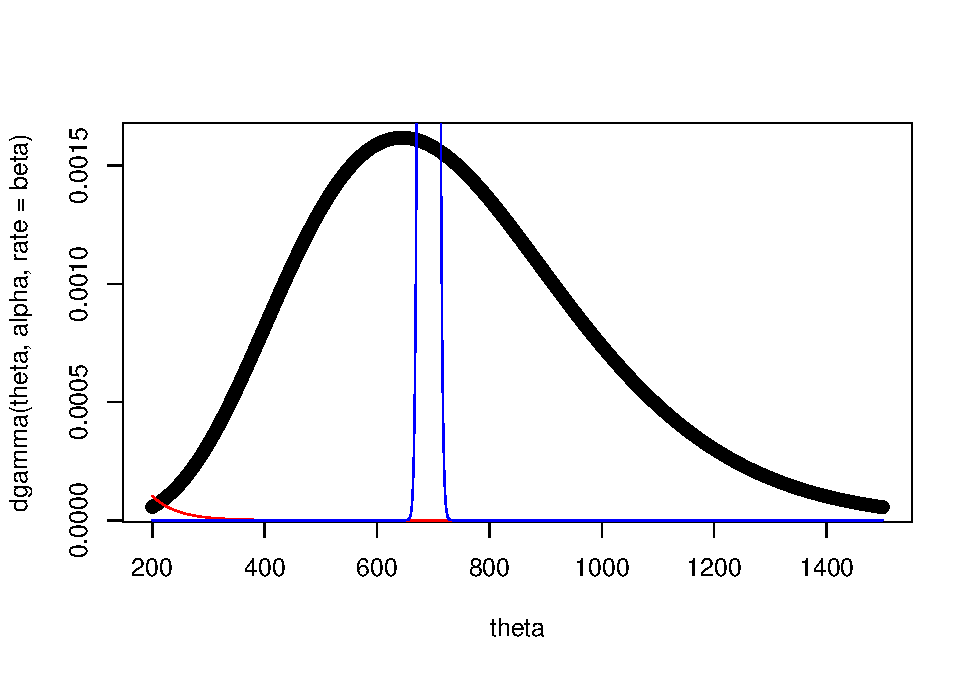
\includegraphics{_main_files/figure-latex/unnamed-chunk-26-1.pdf}

\begin{Shaded}
\begin{Highlighting}[]
 \DocumentationTok{\#\# credible interval of the posterior}
\NormalTok{ pois\_credible}\OtherTok{\textless{}{-}}\FunctionTok{qgamma}\NormalTok{(}\FunctionTok{c}\NormalTok{(.}\DecValTok{025}\NormalTok{,}\FloatTok{0.975}\NormalTok{),alpha}\SpecialCharTok{+}\NormalTok{n}\SpecialCharTok{*}\FunctionTok{mean}\NormalTok{(death),}\AttributeTok{rate=}\NormalTok{beta}\SpecialCharTok{+}\NormalTok{n)}
 \FunctionTok{message}\NormalTok{(}\StringTok{"posterior for empirical gamma interval n=10: "}\NormalTok{,}\FunctionTok{round}\NormalTok{(pois\_credible[}\DecValTok{1}\NormalTok{],}\DecValTok{2}\NormalTok{),}\StringTok{" "}\NormalTok{,}\FunctionTok{round}\NormalTok{(pois\_credible[}\DecValTok{2}\NormalTok{],}\DecValTok{3}\NormalTok{)) }\DocumentationTok{\#\# }
\end{Highlighting}
\end{Shaded}

\begin{verbatim}
## posterior for empirical gamma interval n=10: 675.75 708.338
\end{verbatim}

\begin{Shaded}
\begin{Highlighting}[]
\NormalTok{ jp\_pois\_credible}\OtherTok{\textless{}{-}}\FunctionTok{qgamma}\NormalTok{(}\FunctionTok{c}\NormalTok{(.}\DecValTok{025}\NormalTok{,}\FloatTok{0.975}\NormalTok{),Jalpha}\SpecialCharTok{+}\NormalTok{n}\SpecialCharTok{*}\FunctionTok{mean}\NormalTok{(death),}\AttributeTok{rate=}\NormalTok{Jbeta}\SpecialCharTok{+}\NormalTok{n)}
 \FunctionTok{message}\NormalTok{(}\StringTok{"posterior for Jeffreys\textquotesingle{} gamma interval n=10: "}\NormalTok{,}\FunctionTok{round}\NormalTok{(jp\_pois\_credible[}\DecValTok{1}\NormalTok{],}\DecValTok{2}\NormalTok{),}\StringTok{" "}\NormalTok{,}\FunctionTok{round}\NormalTok{(jp\_pois\_credible[}\DecValTok{2}\NormalTok{],}\DecValTok{3}\NormalTok{)) }\DocumentationTok{\#\# }
\end{Highlighting}
\end{Shaded}

\begin{verbatim}
## posterior for Jeffreys' gamma interval n=10: 674.39 706.934
\end{verbatim}

\begin{Shaded}
\begin{Highlighting}[]
 \DocumentationTok{\#\# produces too small probabilities from Jeffrey\textquotesingle{}s and we can sample here}
\NormalTok{ post\_pois}\OtherTok{\textless{}{-}}\FunctionTok{dgamma}\NormalTok{(theta,alpha}\SpecialCharTok{+}\NormalTok{n}\SpecialCharTok{*}\FunctionTok{mean}\NormalTok{(death),}\AttributeTok{rate=}\NormalTok{beta}\SpecialCharTok{+}\NormalTok{n) }\DocumentationTok{\#\# prob}
\DocumentationTok{\#\#  prediction:  with the grid approach in the Gamma framework does not work for small valued thetas.}
\NormalTok{ theta\_samps}\OtherTok{\textless{}{-}}\FunctionTok{sample}\NormalTok{(theta,}\DecValTok{1000}\NormalTok{,}\AttributeTok{prob=}\NormalTok{post\_pois,}\AttributeTok{replace=}\NormalTok{T)}
\NormalTok{  ytilde\_empiricalPrior}\OtherTok{\textless{}{-}}\FunctionTok{rpois}\NormalTok{(}\DecValTok{1000}\NormalTok{,}\AttributeTok{lambda=}\NormalTok{theta\_samps)}
  \FunctionTok{message}\NormalTok{(}\StringTok{"using the empirical prior, predictive posterior interval"}\NormalTok{)}
\end{Highlighting}
\end{Shaded}

\begin{verbatim}
## using the empirical prior, predictive posterior interval
\end{verbatim}

\begin{Shaded}
\begin{Highlighting}[]
   \FunctionTok{quantile}\NormalTok{(ytilde\_empiricalPrior,}\FunctionTok{c}\NormalTok{(}\FloatTok{0.025}\NormalTok{,}\FloatTok{0.975}\NormalTok{))}
\end{Highlighting}
\end{Shaded}

\begin{verbatim}
##   2.5%  97.5% 
## 637.95 745.00
\end{verbatim}

\begin{Shaded}
\begin{Highlighting}[]
 \DocumentationTok{\#\# direct sampling from posterior.}
\NormalTok{ theta\_post}\OtherTok{\textless{}{-}}\FunctionTok{rgamma}\NormalTok{(}\DecValTok{1000}\NormalTok{,Jalpha}\SpecialCharTok{+}\NormalTok{n}\SpecialCharTok{*}\FunctionTok{mean}\NormalTok{(death),}\AttributeTok{rate=}\NormalTok{Jbeta}\SpecialCharTok{+}\NormalTok{n)}
 
 
\NormalTok{   ytilde}\OtherTok{\textless{}{-}}\FunctionTok{rpois}\NormalTok{(}\DecValTok{1000}\NormalTok{,}\AttributeTok{lambda=}\NormalTok{theta\_post) }
 \DocumentationTok{\#\# probability of the samples }
 \CommentTok{\#prob\_samp\textless{}{-}post[match(samps,theta)]}
  \FunctionTok{summary}\NormalTok{(ytilde) }\DocumentationTok{\#\# we have a wide distribution of predictive values.}
\end{Highlighting}
\end{Shaded}

\begin{verbatim}
##    Min. 1st Qu.  Median    Mean 3rd Qu.    Max. 
##   604.0   671.0   690.0   690.6   709.0   782.0
\end{verbatim}

\begin{Shaded}
\begin{Highlighting}[]
\NormalTok{   post\_pois}\OtherTok{\textless{}{-}}\FunctionTok{dgamma}\NormalTok{(theta\_post,Jalpha}\SpecialCharTok{+}\NormalTok{n}\SpecialCharTok{*}\FunctionTok{mean}\NormalTok{(death),}\AttributeTok{rate=}\NormalTok{Jbeta}\SpecialCharTok{+}\NormalTok{n)}

\DocumentationTok{\#\# for all predictive values,  find the total probability  }
   \DocumentationTok{\#\# int p(x|theta)*p(theta|y) d\textbackslash{}theta  note that p(x|theta) is a function of theta, so we input hte theta grid.}
\NormalTok{ pred.prob}\OtherTok{\textless{}{-}}\FunctionTok{sapply}\NormalTok{(ytilde,}\ControlFlowTok{function}\NormalTok{(x) }\FunctionTok{sum}\NormalTok{(}\FunctionTok{dpois}\NormalTok{(x,}\AttributeTok{lambda =}\NormalTok{ theta\_post)}\SpecialCharTok{*}\NormalTok{post\_pois}\SpecialCharTok{/}\FunctionTok{sum}\NormalTok{(post\_pois)))  }
  
 \FunctionTok{plot}\NormalTok{(ytilde,pred.prob, }\AttributeTok{main=}\StringTok{\textquotesingle{}predictive distribution for future 1986\textquotesingle{}}\NormalTok{)}
 \FunctionTok{abline}\NormalTok{(}\AttributeTok{v=}\FunctionTok{quantile}\NormalTok{(ytilde,}\FunctionTok{c}\NormalTok{(}\FloatTok{0.025}\NormalTok{,}\FloatTok{0.975}\NormalTok{)),}\AttributeTok{col=}\StringTok{\textquotesingle{}red\textquotesingle{}}\NormalTok{)}
\end{Highlighting}
\end{Shaded}

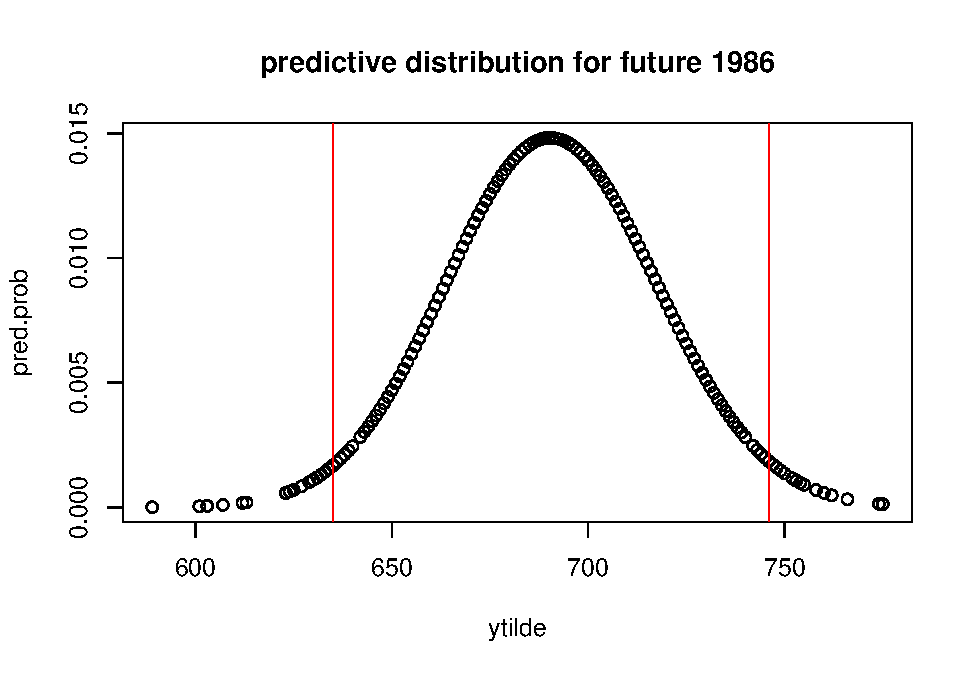
\includegraphics{_main_files/figure-latex/unnamed-chunk-26-2.pdf}

\begin{Shaded}
\begin{Highlighting}[]
\CommentTok{\# lines(theta,post\_pois)}
 \FunctionTok{quantile}\NormalTok{(ytilde,}\FunctionTok{c}\NormalTok{(}\FloatTok{0.025}\NormalTok{,}\FloatTok{0.975}\NormalTok{))}
\end{Highlighting}
\end{Shaded}

\begin{verbatim}
##    2.5%   97.5% 
## 639.000 745.025
\end{verbatim}

\begin{itemize}
\item
  \begin{enumerate}
  \def\labelenumi{(\alph{enumi})}
  \setcounter{enumi}{3}
  \tightlist
  \item
    Using the rate the posterior rate mean is 0.12 estimated from sampling the posterior distribution. For 8 x 10\(^11\) miles flown the deaths are approximately 970 (902, 1039) this is higher than the 1986 observed value.
  \end{enumerate}
\end{itemize}

Note we used Jeffreys' prior here, but an empirical prior is okay

\begin{Shaded}
\begin{Highlighting}[]
\NormalTok{  theta}\OtherTok{=}\FunctionTok{seq}\NormalTok{(}\AttributeTok{from=}\DecValTok{0}\NormalTok{,}\AttributeTok{to=}\FloatTok{0.1}\NormalTok{,}\AttributeTok{by=}\NormalTok{.}\DecValTok{001}\NormalTok{)}
\NormalTok{ miles100}\OtherTok{\textless{}{-}}\NormalTok{death}\SpecialCharTok{/}\NormalTok{rate }\DocumentationTok{\#\# 100 million miles}
\NormalTok{ miles}\OtherTok{\textless{}{-}}\NormalTok{miles100}\SpecialCharTok{*}\DecValTok{100000000}

 


   
  \DocumentationTok{\#\# we must use Jeffreys\textquotesingle{} prior}
\NormalTok{    Jalpha}\OtherTok{=}\FloatTok{0.01}
\NormalTok{  Jbeta}\OtherTok{\textless{}{-}}\FloatTok{0.01}
 \FunctionTok{plot}\NormalTok{(theta,}\FunctionTok{dgamma}\NormalTok{(theta,Jalpha,}\AttributeTok{rate=}\NormalTok{Jbeta),}\AttributeTok{col=}\StringTok{\textquotesingle{}blue\textquotesingle{}}\NormalTok{,}\AttributeTok{xlab=}\StringTok{\textquotesingle{}passanger death rate per miles\textquotesingle{}}\NormalTok{,}\AttributeTok{main=}\StringTok{"Jeffreys\textquotesingle{} prior"}\NormalTok{)}
\FunctionTok{lines}\NormalTok{(theta,}\FunctionTok{dgamma}\NormalTok{(theta,Jalpha}\SpecialCharTok{+}\FunctionTok{sum}\NormalTok{(death),}\AttributeTok{rate=}\NormalTok{Jbeta}\SpecialCharTok{+}\FunctionTok{sum}\NormalTok{(miles)),}\AttributeTok{col=}\StringTok{\textquotesingle{}red\textquotesingle{}}\NormalTok{)}
\end{Highlighting}
\end{Shaded}

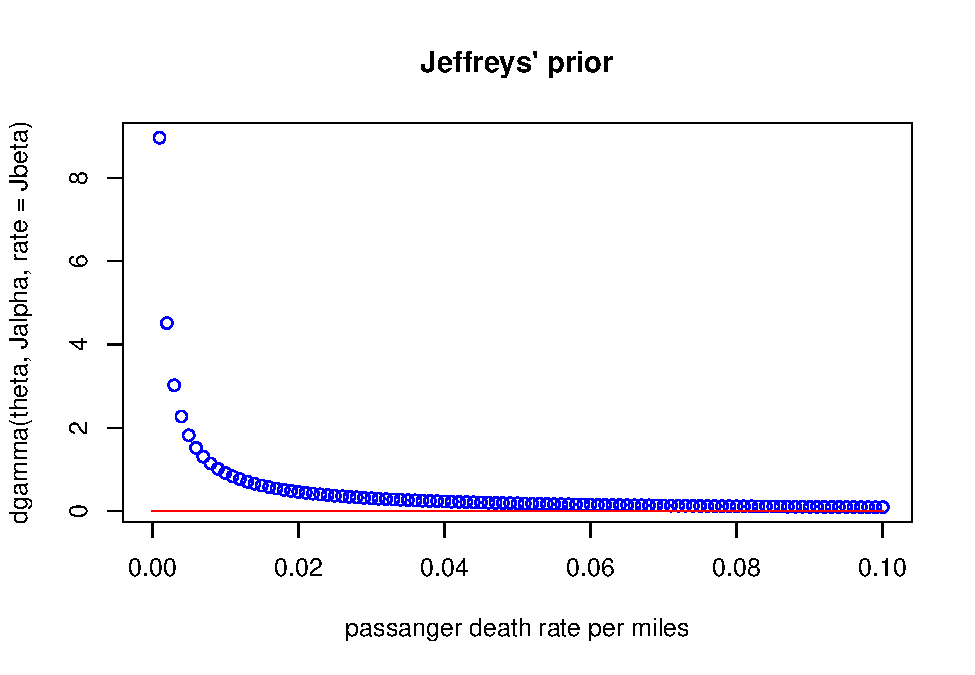
\includegraphics{_main_files/figure-latex/unnamed-chunk-27-1.pdf}

\begin{Shaded}
\begin{Highlighting}[]
 \DocumentationTok{\#\# credible interval of the posterior}
\NormalTok{ pois\_credible}\OtherTok{\textless{}{-}}\FunctionTok{qgamma}\NormalTok{(}\FunctionTok{c}\NormalTok{(.}\DecValTok{025}\NormalTok{,}\FloatTok{0.975}\NormalTok{),Jalpha}\SpecialCharTok{+}\FunctionTok{sum}\NormalTok{(death),}\AttributeTok{rate=}\NormalTok{Jbeta}\SpecialCharTok{+}\FunctionTok{sum}\NormalTok{(miles))}
 \FunctionTok{message}\NormalTok{(}\StringTok{"Jeffreys\textquotesingle{} prior posterior gamma interval n=10: "}\NormalTok{)}
\end{Highlighting}
\end{Shaded}

\begin{verbatim}
## Jeffreys' prior posterior gamma interval n=10:
\end{verbatim}

\begin{Shaded}
\begin{Highlighting}[]
 \FunctionTok{print}\NormalTok{(pois\_credible) }\DocumentationTok{\#\# }
\end{Highlighting}
\end{Shaded}

\begin{verbatim}
## [1] 1.182135e-09 1.239179e-09
\end{verbatim}

\begin{Shaded}
\begin{Highlighting}[]
 \FunctionTok{plot}\NormalTok{(theta,}\FunctionTok{dgamma}\NormalTok{(theta,alpha,}\AttributeTok{rate=}\NormalTok{beta),}\AttributeTok{lty=}\DecValTok{2}\NormalTok{, }\AttributeTok{main=}\StringTok{\textquotesingle{}empirical estimated prior\textquotesingle{}}\NormalTok{)}
\FunctionTok{lines}\NormalTok{(theta,}\FunctionTok{dgamma}\NormalTok{(theta,alpha}\SpecialCharTok{+}\FunctionTok{sum}\NormalTok{(death),}\AttributeTok{rate=}\NormalTok{beta}\SpecialCharTok{+}\FunctionTok{sum}\NormalTok{(miles)),}\AttributeTok{col=}\StringTok{\textquotesingle{}red\textquotesingle{}}\NormalTok{)}
\end{Highlighting}
\end{Shaded}

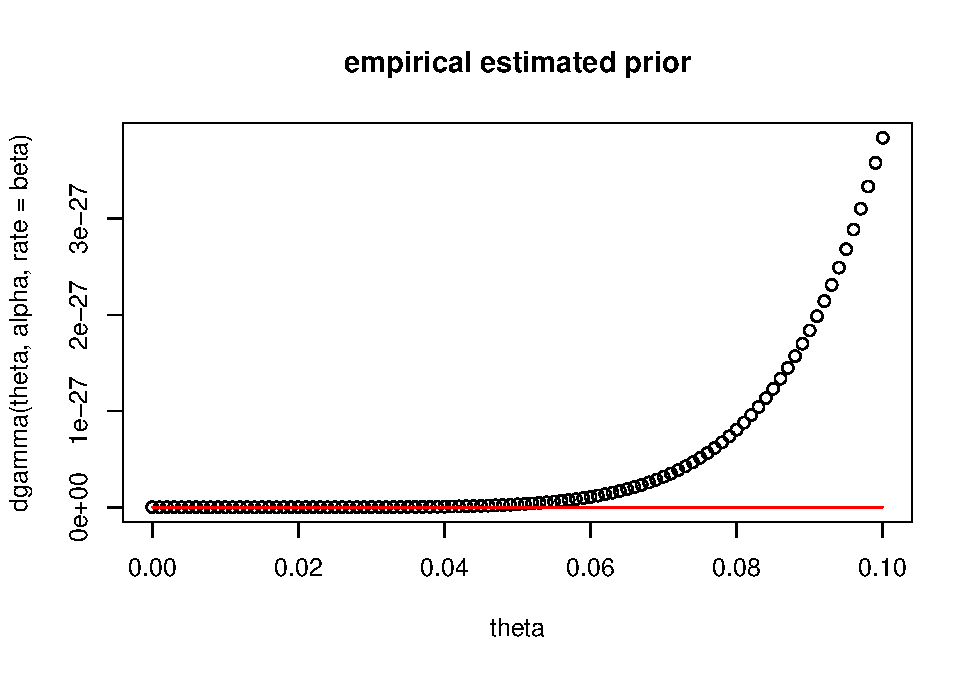
\includegraphics{_main_files/figure-latex/unnamed-chunk-27-2.pdf}

\begin{Shaded}
\begin{Highlighting}[]
 \DocumentationTok{\#\# credible interval of the posterior}


\NormalTok{ theta\_post}\OtherTok{\textless{}{-}}\FunctionTok{rgamma}\NormalTok{(}\DecValTok{1000}\NormalTok{,Jalpha}\SpecialCharTok{+}\FunctionTok{sum}\NormalTok{(death),}\AttributeTok{rate=}\NormalTok{Jbeta}\SpecialCharTok{+}\FunctionTok{sum}\NormalTok{(miles))}
\NormalTok{  y1986}\OtherTok{\textless{}{-}}\FunctionTok{rpois}\NormalTok{(}\DecValTok{1000}\NormalTok{,}\FloatTok{8e+11}\SpecialCharTok{*}\NormalTok{theta\_post) }\DocumentationTok{\#\# use in the likelihood}
  \FunctionTok{message}\NormalTok{(}\StringTok{" 8,000 per 100 million miles flown has passanger death : Gamma posterior \& Jeffreys\textquotesingle{} prior"}\NormalTok{)}
\end{Highlighting}
\end{Shaded}

\begin{verbatim}
##  8,000 per 100 million miles flown has passanger death : Gamma posterior & Jeffreys' prior
\end{verbatim}

\begin{Shaded}
\begin{Highlighting}[]
 \FunctionTok{print}\NormalTok{(}\FunctionTok{sort}\NormalTok{(y1986)[}\FunctionTok{c}\NormalTok{(}\DecValTok{25}\NormalTok{,}\DecValTok{976}\NormalTok{)])}
\end{Highlighting}
\end{Shaded}

\begin{verbatim}
## [1]  902 1037
\end{verbatim}

\hypertarget{question-21}{%
\subsection{Question 21}\label{question-21}}

estimate percentage of adult population in each state (excluding alaska and hawaii) who label themselves as very liberal. plot estimate vs.~obama's vote share in 2008.

For each state we measure \(y_j\sim Pois(n_j\theta_j)\) from section 2.7 where y is the number of adult population who identify themselves as \emph{very liberal} in ideology for a given state.

we do not have population of each state, but we do have the number of respondents of each state, and denote \(n_j\) as the integer representing the total respondents.

Alternatively, we do have census density category for each state (1-5) which can account for the populaiton density.

\begin{itemize}
\item
  \begin{enumerate}
  \def\labelenumi{(\alph{enumi})}
  \tightlist
  \item
    graph the proportion of liberal in each state vs obama vote share. here the proportion of liberal votes was weighted by the total respondents
  \end{enumerate}
\end{itemize}

we see that the highest proportion of very liberal polls is associated with the states with the highest obama percentage of votes in CA, NY, WA, and IL. Conversely we see that WY UT, OK are very red states with low polls in very liberal voters, with the lowest support for obama.

For those that identify as \emph{liberal} we see a much linear trend.

\begin{Shaded}
\begin{Highlighting}[]
 \FunctionTok{library}\NormalTok{(foreign)}
 \FunctionTok{library}\NormalTok{(dplyr)}
\end{Highlighting}
\end{Shaded}

\begin{verbatim}
## 
## Attaching package: 'dplyr'
\end{verbatim}

\begin{verbatim}
## The following objects are masked from 'package:stats':
## 
##     filter, lag
\end{verbatim}

\begin{verbatim}
## The following objects are masked from 'package:base':
## 
##     intersect, setdiff, setequal, union
\end{verbatim}

\begin{Shaded}
\begin{Highlighting}[]
 \FunctionTok{library}\NormalTok{(magrittr)}
 \FunctionTok{library}\NormalTok{(ggplot2)}
\CommentTok{\#polls\textless{}{-}read.dta("C:/Users/UOSC/Documents/Keck{-}graduate{-}school/PM590{-}Bayesian/bookdown{-}files/pew\_research\_center\_june\_elect\_wknd\_data.dta")}
\NormalTok{polls}\OtherTok{\textless{}{-}}\FunctionTok{read.dta}\NormalTok{(}\StringTok{"C:/Users/antho/Documents/Keck{-}graduate{-}school/PM590{-}Bayesian/bookdown{-}files/pew\_research\_center\_june\_elect\_wknd\_data.dta"}\NormalTok{)}
 \CommentTok{\#proportion of very liberal}
\FunctionTok{table}\NormalTok{(polls}\SpecialCharTok{$}\NormalTok{ideo)}
\end{Highlighting}
\end{Shaded}

\begin{verbatim}
## 
## missing/not asked very conservative      conservative          moderate 
##                 0              2417              9795             11197 
##           liberal      very liberal        dk/refused 
##              4535              1470              1380
\end{verbatim}

\begin{Shaded}
\begin{Highlighting}[]
 \DocumentationTok{\#\# adult pop}
\FunctionTok{table}\NormalTok{(polls}\SpecialCharTok{$}\NormalTok{age)}
\end{Highlighting}
\end{Shaded}

\begin{verbatim}
## 
##  18  19  20  21  22  23  24  25  26  27  28  29  30  31  32  33  34  35  36  37 
## 628 431 363 341 316 374 355 343 406 337 391 398 446 366 375 378 334 398 417 482 
##  38  39  40  41  42  43  44  45  46  47  48  49  50  51  52  53  54  55  56  57 
## 509 441 617 464 542 470 529 582 571 615 639 593 891 598 727 618 639 731 600 541 
##  58  59  60  61  62  63  64  65  66  67  68  69  70  71  72  73  74  75  76  77 
## 662 561 799 584 590 419 489 596 422 426 373 368 494 294 358 266 256 323 260 269 
##  78  79  80  81  82  83  84  85  86  87  88  89  90  91  92  93  94  95  96  97 
## 233 220 337 195 179 143 126 132 106  97  81  73  62  25  21  13   9   7   2  18 
##  99 
## 517
\end{verbatim}

\begin{Shaded}
\begin{Highlighting}[]
\FunctionTok{table}\NormalTok{(polls}\SpecialCharTok{$}\NormalTok{age2)}
\end{Highlighting}
\end{Shaded}

\begin{verbatim}
## 
##       18-29       30-49       50-64         65+ dk\\refused 
##        4683        9768        9449        6784         517
\end{verbatim}

\begin{Shaded}
\begin{Highlighting}[]
\DocumentationTok{\#\# each state}
 \FunctionTok{table}\NormalTok{(polls}\SpecialCharTok{$}\NormalTok{state)}
\end{Highlighting}
\end{Shaded}

\begin{verbatim}
## 
##        alabama         alaska        arizona       arkansas     california 
##            624              0            542            307           2854 
##       colorado    connecticut       delaware  washington dc        florida 
##            468            395            119             62           1747 
##        georgia         hawaii          idaho       illinois        indiana 
##           1023              1            140           1130            829 
##           iowa         kansas       kentucky      louisiana          maine 
##            441            329            523            603            154 
##       maryland  massachusetts       michigan      minnesota    mississippi 
##            593            685           1000            711            264 
##       missouri        montana       nebraska         nevada  new hampshire 
##            780             91            215            202            160 
##     new jersey     new mexico       new york north carolina   north dakota 
##            870            219           1701           1055            120 
##           ohio       oklahoma         oregon   pennsylvania   rhode island 
##           1404            431            468           1591            131 
## south carolina   south dakota      tennessee          texas           utah 
##            458             93            745           1919            284 
##        vermont       virginia     washington  west virginia      wisconsin 
##            115            896            668            270            742 
##        wyoming 
##             29
\end{verbatim}

\begin{Shaded}
\begin{Highlighting}[]
 \CommentTok{\# drop AL and HA}
\NormalTok{polls}\OtherTok{\textless{}{-}}\NormalTok{polls[}\FunctionTok{which}\NormalTok{(polls}\SpecialCharTok{$}\NormalTok{state}\SpecialCharTok{!=}\StringTok{"alaska"} \SpecialCharTok{\&}\NormalTok{ polls}\SpecialCharTok{$}\NormalTok{state}\SpecialCharTok{!=}\StringTok{"hawaii"}\NormalTok{),] }
\CommentTok{\# average the points that are missing.}
\NormalTok{polls}\SpecialCharTok{$}\NormalTok{density[}\FunctionTok{which}\NormalTok{(}\FunctionTok{is.na}\NormalTok{(polls}\SpecialCharTok{$}\NormalTok{density))]}\OtherTok{\textless{}{-}}\FunctionTok{mean}\NormalTok{(polls}\SpecialCharTok{$}\NormalTok{density[}\FunctionTok{which}\NormalTok{(}\SpecialCharTok{!}\FunctionTok{is.na}\NormalTok{(polls}\SpecialCharTok{$}\NormalTok{density))])}

\CommentTok{\#ele\textless{}{-}read.csv("C:/Users/UOSC/Documents/Keck{-}graduate{-}school/PM590{-}Bayesian/bookdown{-}files/2008ElectionResult.csv")}
\NormalTok{ele}\OtherTok{\textless{}{-}}\FunctionTok{read.csv}\NormalTok{(}\StringTok{"C:/Users/antho/Documents/Keck{-}graduate{-}school/PM590{-}Bayesian/bookdown{-}files/2008ElectionResult.csv"}\NormalTok{)}
\NormalTok{ele}\OtherTok{\textless{}{-}}\NormalTok{ele[}\FunctionTok{which}\NormalTok{(ele}\SpecialCharTok{$}\NormalTok{state}\SpecialCharTok{!=}\StringTok{"Alaska"}\SpecialCharTok{\&}\NormalTok{ ele}\SpecialCharTok{$}\NormalTok{state}\SpecialCharTok{!=}\StringTok{"Hawaii"}\NormalTok{),]}
\NormalTok{ele}\SpecialCharTok{$}\NormalTok{state}\OtherTok{\textless{}{-}}\FunctionTok{tolower}\NormalTok{(ele}\SpecialCharTok{$}\NormalTok{state)}
\DocumentationTok{\#\# graph poprotion liberal in each state vs obama vote share scatter.}

\NormalTok{yj}\OtherTok{\textless{}{-}}\FunctionTok{as.data.frame.matrix}\NormalTok{(}\FunctionTok{table}\NormalTok{(polls}\SpecialCharTok{$}\NormalTok{state,polls}\SpecialCharTok{$}\NormalTok{ideo))}
\NormalTok{nj}\OtherTok{\textless{}{-}}\FunctionTok{as.data.frame.matrix}\NormalTok{(}\FunctionTok{table}\NormalTok{(polls}\SpecialCharTok{$}\NormalTok{state,polls}\SpecialCharTok{$}\NormalTok{density))}
\DocumentationTok{\#\# ideology}
\FunctionTok{head}\NormalTok{(yj)}
\end{Highlighting}
\end{Shaded}

\begin{verbatim}
##            missing/not asked very conservative conservative moderate liberal
## alabama                    0                82          254      165      48
## alaska                     0                 0            0        0       0
## arizona                    0                33          152      201      95
## arkansas                   0                30          115      101      29
## california                 0               178          728     1054     549
## colorado                   0                31          134      165      96
##            very liberal dk/refused
## alabama              30         38
## alaska                0          0
## arizona              28         24
## arkansas              7         22
## california          179        121
## colorado             27         12
\end{verbatim}

\begin{Shaded}
\begin{Highlighting}[]
\DocumentationTok{\#\# density}
\FunctionTok{head}\NormalTok{(nj)}
\end{Highlighting}
\end{Shaded}

\begin{verbatim}
##              1   2 2.8302567571921   3   4   5
## alabama    247 196               9 170   2   0
## alaska       0   0               0   0   0   0
## arizona    247   1               0 294   0   0
## arkansas   148 120               4  35   0   0
## california 455 496              19 438 566 880
## colorado   123 157               7 101   1  79
\end{verbatim}

\begin{Shaded}
\begin{Highlighting}[]
\NormalTok{ tally}\OtherTok{\textless{}{-}}\NormalTok{polls}\SpecialCharTok{\%\textgreater{}\%}\FunctionTok{group\_by}\NormalTok{(state,ideo)}\SpecialCharTok{\%\textgreater{}\%}\FunctionTok{summarize}\NormalTok{(}\AttributeTok{n=}\FunctionTok{n}\NormalTok{())}
\end{Highlighting}
\end{Shaded}

\begin{verbatim}
## `summarise()` has grouped output by 'state'. You can override using the
## `.groups` argument.
\end{verbatim}

\begin{Shaded}
\begin{Highlighting}[]
\NormalTok{ statetotal}\OtherTok{\textless{}{-}}\NormalTok{tally}\SpecialCharTok{\%\textgreater{}\%}\FunctionTok{group\_by}\NormalTok{(state)}\SpecialCharTok{\%\textgreater{}\%}\FunctionTok{summarise}\NormalTok{(}\AttributeTok{statetotal=}\FunctionTok{sum}\NormalTok{(n))}
\NormalTok{ tally}\OtherTok{\textless{}{-}}\FunctionTok{left\_join}\NormalTok{(tally,statetotal,}\AttributeTok{by=}\StringTok{\textquotesingle{}state\textquotesingle{}}\NormalTok{)}
 \DocumentationTok{\#\# average the density of the polling regions by state taking the density of each zip code (category 1{-}5)}
\NormalTok{ densit}\OtherTok{\textless{}{-}}\NormalTok{polls}\SpecialCharTok{\%\textgreater{}\%}\FunctionTok{group\_by}\NormalTok{(state)}\SpecialCharTok{\%\textgreater{}\%}\FunctionTok{summarize}\NormalTok{(}\AttributeTok{density=}\FunctionTok{mean}\NormalTok{(density))}
 
 \CommentTok{\# highest states with highest density}
\NormalTok{ densit[}\FunctionTok{order}\NormalTok{(densit}\SpecialCharTok{$}\NormalTok{density,}\AttributeTok{decreasing =}\NormalTok{ T),]}
\end{Highlighting}
\end{Shaded}

\begin{verbatim}
## # A tibble: 49 x 2
##    state         density
##    <fct>           <dbl>
##  1 washington dc    4.95
##  2 new jersey       3.99
##  3 rhode island     3.93
##  4 maryland         3.62
##  5 new york         3.60
##  6 massachusetts    3.58
##  7 connecticut      3.55
##  8 illinois         3.42
##  9 california       3.32
## 10 ohio             3.32
## # ... with 39 more rows
## # i Use `print(n = ...)` to see more rows
\end{verbatim}

\begin{Shaded}
\begin{Highlighting}[]
\NormalTok{ tally}\OtherTok{\textless{}{-}}\FunctionTok{left\_join}\NormalTok{(tally,densit,}\AttributeTok{by=}\StringTok{\textquotesingle{}state\textquotesingle{}}\NormalTok{)}
\NormalTok{  tally}\SpecialCharTok{$}\NormalTok{popdensity}\OtherTok{\textless{}{-}}\NormalTok{tally}\SpecialCharTok{$}\NormalTok{n}\SpecialCharTok{/}\NormalTok{tally}\SpecialCharTok{$}\NormalTok{density}
\NormalTok{    tally}\SpecialCharTok{$}\NormalTok{stateperc}\OtherTok{\textless{}{-}}\DecValTok{100}\SpecialCharTok{*}\NormalTok{tally}\SpecialCharTok{$}\NormalTok{n}\SpecialCharTok{/}\NormalTok{tally}\SpecialCharTok{$}\NormalTok{statetotal}
\NormalTok{    tally}\SpecialCharTok{$}\NormalTok{stateperc\_density}\OtherTok{\textless{}{-}}\DecValTok{100}\SpecialCharTok{*}\NormalTok{tally}\SpecialCharTok{$}\NormalTok{n}\SpecialCharTok{/}\NormalTok{(tally}\SpecialCharTok{$}\NormalTok{statetotal}\SpecialCharTok{*}\NormalTok{tally}\SpecialCharTok{$}\NormalTok{density)}

  

\NormalTok{tt}\OtherTok{\textless{}{-}}\FunctionTok{left\_join}\NormalTok{(ele,tally,}\AttributeTok{by=}\StringTok{"state"}\NormalTok{)}

\FunctionTok{ggplot}\NormalTok{(tt[}\FunctionTok{which}\NormalTok{(tt}\SpecialCharTok{$}\NormalTok{ideo}\SpecialCharTok{==}\StringTok{\textquotesingle{}very liberal\textquotesingle{}}\NormalTok{),],}\FunctionTok{aes}\NormalTok{(}\AttributeTok{x=}\NormalTok{stateperc,}\AttributeTok{y=}\NormalTok{vote\_Obama\_pct,}\AttributeTok{label=}\NormalTok{state))}\SpecialCharTok{+}\FunctionTok{geom\_point}\NormalTok{(}\AttributeTok{size=}\DecValTok{3}\NormalTok{)}\SpecialCharTok{+}\FunctionTok{geom\_text}\NormalTok{(}\AttributeTok{hjust=}\DecValTok{0}\NormalTok{,}\AttributeTok{vjust=}\DecValTok{0}\NormalTok{)}\SpecialCharTok{+}\FunctionTok{ggtitle}\NormalTok{(}\StringTok{"very liberal proportion vs. obama vote (\%)"}\NormalTok{)}
\end{Highlighting}
\end{Shaded}

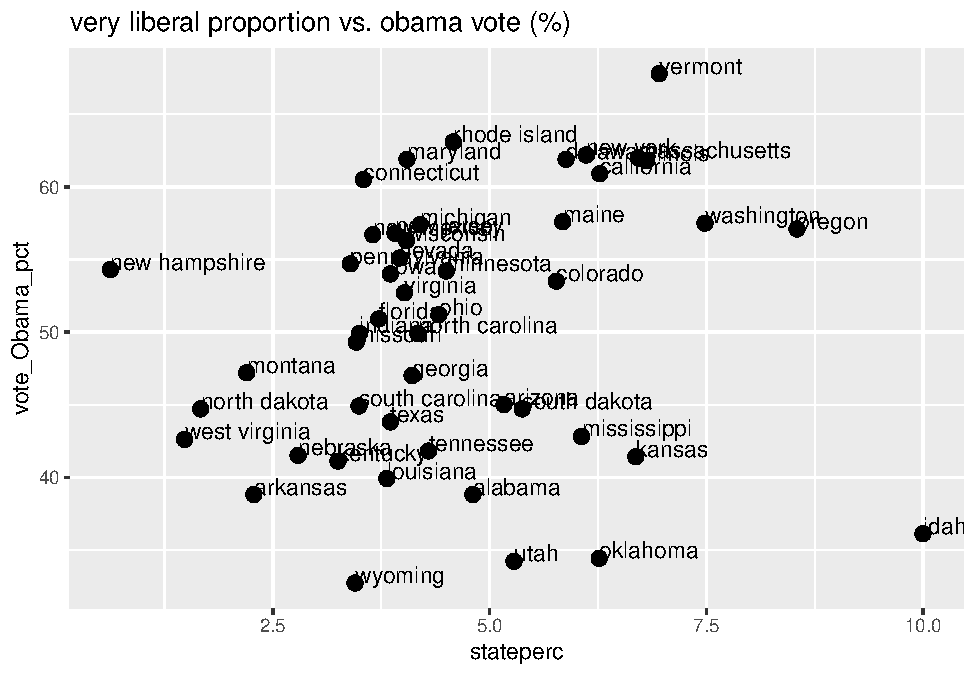
\includegraphics{_main_files/figure-latex/unnamed-chunk-28-1.pdf}

\begin{Shaded}
\begin{Highlighting}[]
\FunctionTok{ggplot}\NormalTok{(tt[}\FunctionTok{which}\NormalTok{(tt}\SpecialCharTok{$}\NormalTok{ideo}\SpecialCharTok{==}\StringTok{\textquotesingle{}liberal\textquotesingle{}}\NormalTok{),],}\FunctionTok{aes}\NormalTok{(}\AttributeTok{x=}\NormalTok{stateperc,}\AttributeTok{y=}\NormalTok{vote\_Obama\_pct,}\AttributeTok{label=}\NormalTok{state))}\SpecialCharTok{+}\FunctionTok{geom\_point}\NormalTok{(}\AttributeTok{size=}\DecValTok{3}\NormalTok{)}\SpecialCharTok{+}\FunctionTok{geom\_text}\NormalTok{(}\AttributeTok{hjust=}\DecValTok{0}\NormalTok{,}\AttributeTok{vjust=}\DecValTok{0}\NormalTok{)}\SpecialCharTok{+}\FunctionTok{ggtitle}\NormalTok{(}\StringTok{"liberal proportion vs. obama vote (\%)"}\NormalTok{)}
\end{Highlighting}
\end{Shaded}

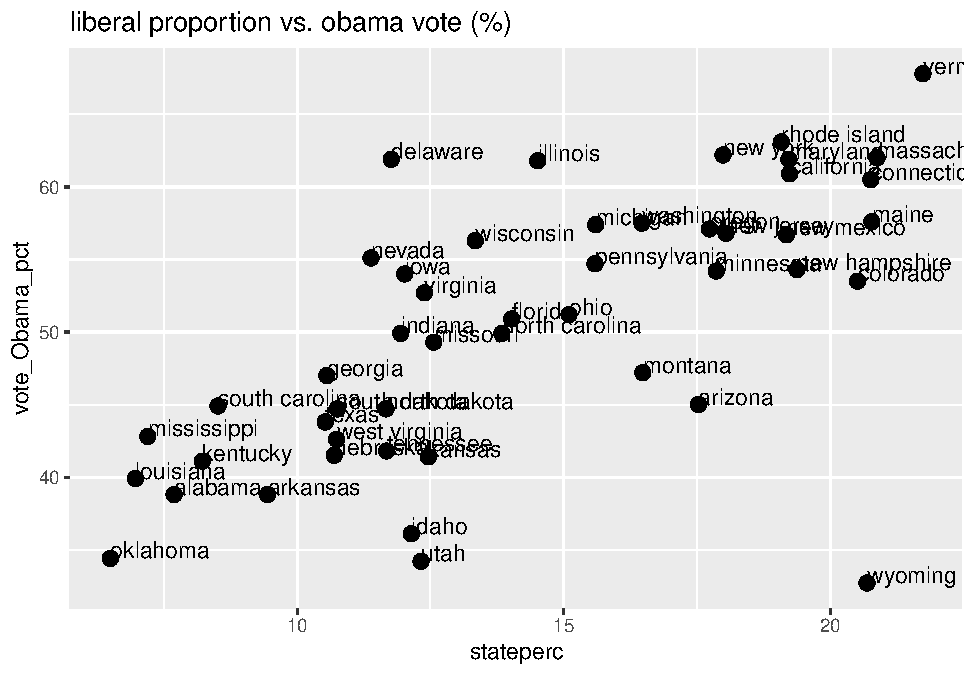
\includegraphics{_main_files/figure-latex/unnamed-chunk-28-2.pdf}

\begin{itemize}
\item
  \begin{enumerate}
  \def\labelenumi{(\alph{enumi})}
  \setcounter{enumi}{1}
  \tightlist
  \item
    Graph the posterior Bayes mean vs.~the Obama vote share.
    In order to construct the prior we use equations (2.17, 2.18) where we match the moments from the prior predictive distribution to the observed data for each state. \(p(\tilde{y})\sim Neg-Bin(\alpha, \beta)\) follows a negative binomial distribution.
  \end{enumerate}
\end{itemize}

\begin{Shaded}
\begin{Highlighting}[]
 \DocumentationTok{\#\# we need to understand the underlying rates in a prior for gamma given multiple states.}
\NormalTok{ vl}\OtherTok{\textless{}{-}}\FunctionTok{subset}\NormalTok{(tally,tally}\SpecialCharTok{$}\NormalTok{ideo}\SpecialCharTok{==}\StringTok{\textquotesingle{}very liberal\textquotesingle{}}\NormalTok{)}
  \FunctionTok{hist}\NormalTok{(vl}\SpecialCharTok{$}\NormalTok{stateperc, }\AttributeTok{xlab=}\StringTok{"very lib. (\%)"}\NormalTok{, }\AttributeTok{ylab=}\StringTok{"frequency"}\NormalTok{)}
\end{Highlighting}
\end{Shaded}

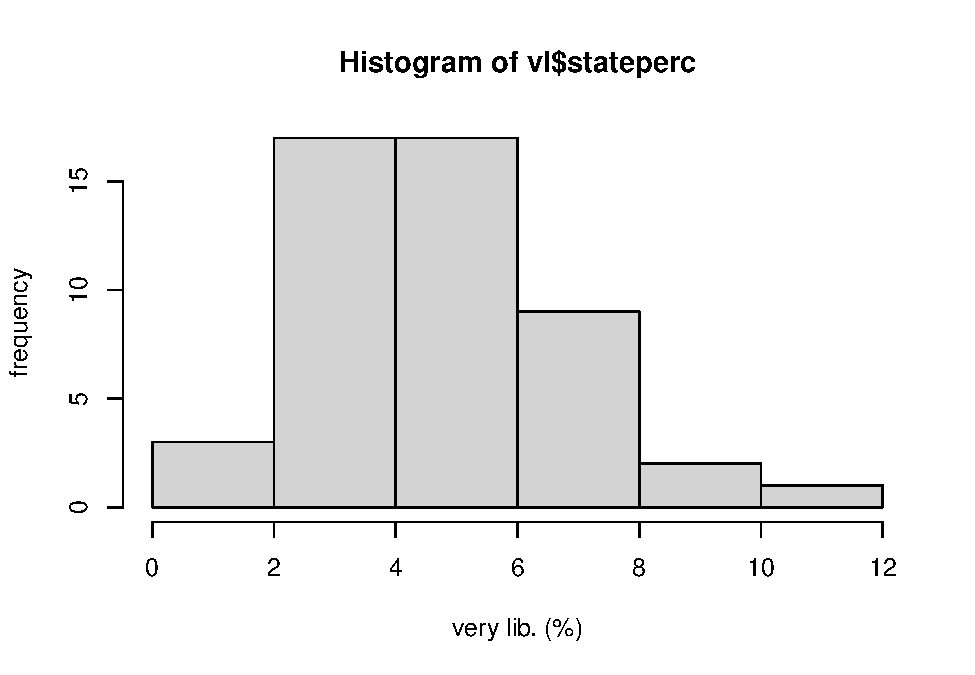
\includegraphics{_main_files/figure-latex/unnamed-chunk-29-1.pdf}

\begin{Shaded}
\begin{Highlighting}[]
  \DocumentationTok{\#\# for each state we must identify the estimate}
  
  \DocumentationTok{\#\# empircal bayesian prior for percentage of respondents}
\NormalTok{ emp.mean}\OtherTok{\textless{}{-}}\FunctionTok{mean}\NormalTok{(vl}\SpecialCharTok{$}\NormalTok{stateperc)}
\NormalTok{ emp.var}\OtherTok{\textless{}{-}}\FunctionTok{var}\NormalTok{(vl}\SpecialCharTok{$}\NormalTok{stateperc)}

\NormalTok{  beta}\OtherTok{=}\NormalTok{beta}\OtherTok{\textless{}{-}}\DecValTok{1}\SpecialCharTok{/}\NormalTok{((}\FunctionTok{var}\NormalTok{(vl}\SpecialCharTok{$}\NormalTok{stateperc)}\SpecialCharTok{{-}}\NormalTok{(}\FunctionTok{mean}\NormalTok{(}\DecValTok{1}\SpecialCharTok{/}\NormalTok{vl}\SpecialCharTok{$}\NormalTok{density))}\SpecialCharTok{*}\NormalTok{emp.mean)}\SpecialCharTok{/}\NormalTok{(emp.mean))}
\NormalTok{  alpha }\OtherTok{=}\NormalTok{ beta}\SpecialCharTok{*}\NormalTok{emp.mean}
  
\NormalTok{alpha\_unif}\OtherTok{=} \FloatTok{0.01}
\NormalTok{beta\_unif }\OtherTok{=} \FloatTok{0.01}

\FunctionTok{qgamma}\NormalTok{(}\FunctionTok{c}\NormalTok{(}\FloatTok{0.025}\NormalTok{,}\FloatTok{0.975}\NormalTok{),alpha,beta)}
\end{Highlighting}
\end{Shaded}

\begin{verbatim}
## [1] 2.422521 7.788166
\end{verbatim}

\begin{Shaded}
\begin{Highlighting}[]
\FunctionTok{quantile}\NormalTok{(tally}\SpecialCharTok{$}\NormalTok{prop,}\FunctionTok{c}\NormalTok{(}\FloatTok{0.025}\NormalTok{,}\FloatTok{0.975}\NormalTok{))  }
\end{Highlighting}
\end{Shaded}

\begin{verbatim}
## Warning: Unknown or uninitialised column: `prop`.
\end{verbatim}

\begin{verbatim}
##  2.5% 97.5% 
##    NA    NA
\end{verbatim}

\begin{Shaded}
\begin{Highlighting}[]
\NormalTok{  theta}\OtherTok{=}\FunctionTok{seq}\NormalTok{(}\AttributeTok{from=}\DecValTok{0}\NormalTok{,}\AttributeTok{to=}\FloatTok{0.1}\NormalTok{,}\AttributeTok{by=}\NormalTok{.}\DecValTok{001}\NormalTok{)}
 \FunctionTok{plot}\NormalTok{(theta,}\FunctionTok{dgamma}\NormalTok{(theta,alpha,}\AttributeTok{rate=}\NormalTok{beta),}\AttributeTok{lty=}\DecValTok{2}\NormalTok{, }\AttributeTok{xlab=}\StringTok{\textquotesingle{}very liberal voters by state\textquotesingle{}}\NormalTok{)}
\FunctionTok{lines}\NormalTok{(theta,}\FunctionTok{dgamma}\NormalTok{(theta,alpha\_unif,}\AttributeTok{rate=}\NormalTok{beta\_unif),}\AttributeTok{col=}\StringTok{\textquotesingle{}red\textquotesingle{}}\NormalTok{)}
\end{Highlighting}
\end{Shaded}

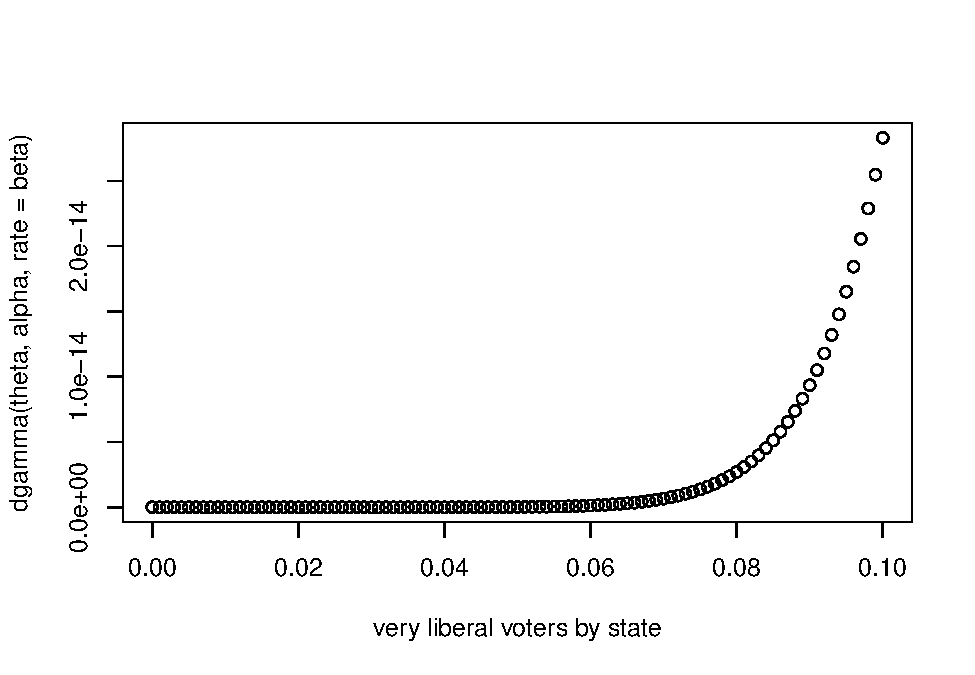
\includegraphics{_main_files/figure-latex/unnamed-chunk-29-2.pdf}

\begin{Shaded}
\begin{Highlighting}[]
\NormalTok{dat}\OtherTok{\textless{}{-}}\NormalTok{tt[}\FunctionTok{which}\NormalTok{(tt}\SpecialCharTok{$}\NormalTok{ideo}\SpecialCharTok{==}\StringTok{\textquotesingle{}very liberal\textquotesingle{}}\NormalTok{),]}


\NormalTok{post}\OtherTok{\textless{}{-}}\ControlFlowTok{function}\NormalTok{(theta,yj,nj)\{}
\NormalTok{ dd}\OtherTok{\textless{}{-}}\FunctionTok{dgamma}\NormalTok{(theta,alpha}\SpecialCharTok{+}\NormalTok{yj,}\AttributeTok{rate=}\NormalTok{beta}\SpecialCharTok{+}\NormalTok{nj)}
 \FunctionTok{return}\NormalTok{(dd)}
\NormalTok{\}}
\NormalTok{postMean}\OtherTok{\textless{}{-}}\ControlFlowTok{function}\NormalTok{(alpha,yj,beta,nj)\{}
\NormalTok{  (alpha}\SpecialCharTok{+}\NormalTok{yj)}\SpecialCharTok{/}\NormalTok{(beta}\SpecialCharTok{+}\NormalTok{nj)}
\NormalTok{  \}}
 
\NormalTok{post\_thetaj}\OtherTok{\textless{}{-}} \FunctionTok{postMean}\NormalTok{(alpha\_unif,dat}\SpecialCharTok{$}\NormalTok{n,beta\_unif,dat}\SpecialCharTok{$}\NormalTok{density)}
\NormalTok{pp}\OtherTok{\textless{}{-}}\FunctionTok{data.frame}\NormalTok{(}\AttributeTok{state=}\NormalTok{dat}\SpecialCharTok{$}\NormalTok{state,}\AttributeTok{post=}\FunctionTok{postMean}\NormalTok{(alpha\_unif,dat}\SpecialCharTok{$}\NormalTok{n,beta\_unif,dat}\SpecialCharTok{$}\NormalTok{density))}
\NormalTok{tt2}\OtherTok{\textless{}{-}}\FunctionTok{left\_join}\NormalTok{(ele,pp,}\AttributeTok{by=}\StringTok{"state"}\NormalTok{)}
\FunctionTok{ggplot}\NormalTok{(tt2,}\FunctionTok{aes}\NormalTok{(}\AttributeTok{x=}\NormalTok{post,}\AttributeTok{y=}\NormalTok{vote\_Obama\_pct,}\AttributeTok{label=}\NormalTok{state))}\SpecialCharTok{+}\FunctionTok{geom\_point}\NormalTok{(}\AttributeTok{size=}\DecValTok{3}\NormalTok{)}\SpecialCharTok{+}\FunctionTok{geom\_text}\NormalTok{(}\AttributeTok{hjust=}\DecValTok{0}\NormalTok{,}\AttributeTok{vjust=}\DecValTok{0}\NormalTok{)}
\end{Highlighting}
\end{Shaded}

\begin{verbatim}
## Warning: Removed 1 rows containing missing values (geom_point).
\end{verbatim}

\begin{verbatim}
## Warning: Removed 1 rows containing missing values (geom_text).
\end{verbatim}

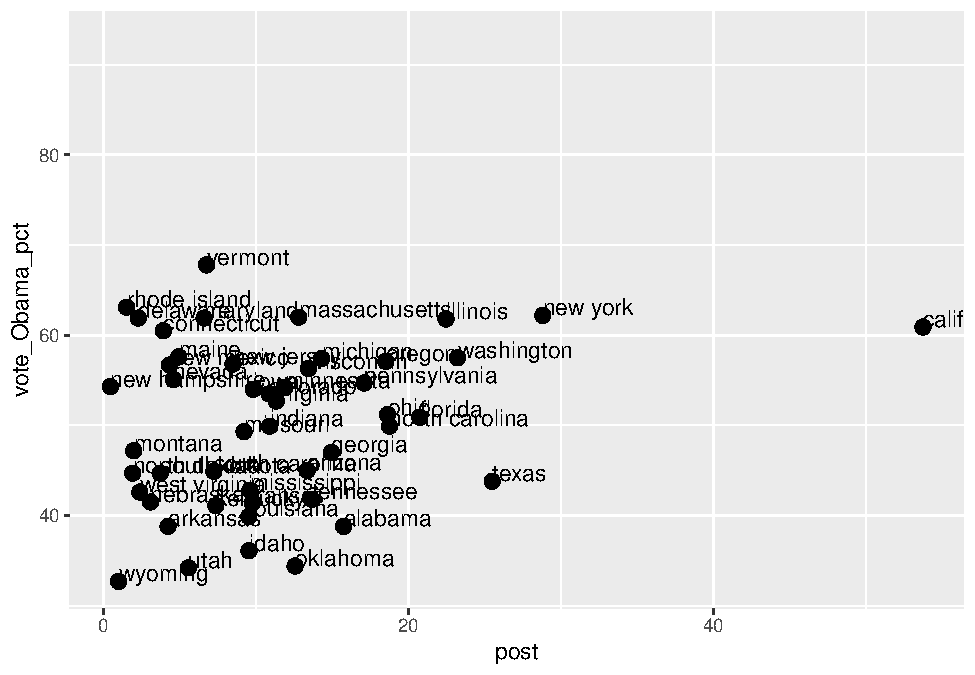
\includegraphics{_main_files/figure-latex/unnamed-chunk-29-3.pdf}

\hypertarget{chapter-3}{%
\chapter{Chapter 3}\label{chapter-3}}

\hypertarget{exercises-2}{%
\chapter*{Exercises}\label{exercises-2}}
\addcontentsline{toc}{chapter}{Exercises}

\hypertarget{question-1-1}{%
\section{Question 1}\label{question-1-1}}

\begin{itemize}
\item
  \begin{enumerate}
  \def\labelenumi{(\alph{enumi})}
  \tightlist
  \item
    find the marginal posterior of \(\alpha = \theta_1/(\theta_1+\theta_2)\)
    We need to find the joint posterior of \(\theta_1, \theta_2\) and then perform a change of variables to (\(\alpha,\beta)\). Let the prior \(p(\theta)=Diri(a_1,...,a_J)\) where y follows a multinomial likelihood.
    \[
    \begin{aligned}
    p(\theta | y) &= \prod \theta_j^{y_j}\theta_j^{a_j-1}\\
    &= \prod \theta_j^{y_j+a_j-1}\\
    & \sim Diri(y_j+a_j)\\
    \end{aligned}
    \]
    The posterior follows a Dirichlet distribution, but we are interested only in the \(\theta_1,\theta_2\) parameters and need to find the marginal posterior of these subvectors. The prior marginal follows for \(a_0= \sum a_i\) and \(y_0= \sum y_i\)
  \end{enumerate}
\end{itemize}

From the Appendix A the joint posterior of the sub vector is
\[
\begin{aligned}
(\theta_1, \theta_2, 1-\theta_1-\theta_2| y ) &\sim Diri(y_1+a_1,y_2+a_2, a_0+y_0-y_1-y_2-a_1-a_2)\\
&p(\theta_1,\theta_2,1-\theta_1-\theta_2) \propto \theta_1^{y_1+a_1-1}\theta_2^{y_2+a_2-1}(1-\theta_1-\theta_2)^{a_0+y_0-y_1-y_2-a_1-a_2-1}\\
\end{aligned}
\]
In order to find the distribution of \(\theta_1/(\theta_1+\theta_2)\) we need the jacobian, let (\(\alpha,\beta) = (\theta_1/(\theta_1+\theta_2) , \theta_1+\theta_2)\).
Rearranging the terms we have \(\theta_1 = \alpha*\beta\) , and \(\theta_2= \beta(1-\alpha)\)
\[
\begin{aligned}
|J| &= \begin{bmatrix}
 \beta & \alpha \\
 -\beta & (1-\alpha)\\
\end{bmatrix} \\
 &=|\beta|\\
\end{aligned}
\]
where \(a'_0 = \sum a_i -a_1 -a_2\), and \(y'_0 =\sum y_i-y_1-y_2\)
\[
\begin{aligned}
p(\alpha,\beta) &= (\alpha*\beta)^{y_1+a_1-1}(\beta(1-\alpha))^{y_2+a_2-1}(1-\alpha*\beta-\beta(1-\alpha))^{a'_0+y'_0-1}|\beta|\\
&=\alpha^{y_1+a_1-1}(1-\alpha)^{y_2+a_2-1}\beta^{y_1+a_1+y_2+a_2-1}(1-\beta)^{a'_0+y'_0-1}\\
&= Beta(y_1+a_1,y_2+a_2)Beta(y_1+a_1+y_2+a_2, a'_0+y'_0)\\
\end{aligned}
\]
By factorization we integrate out with respect \(\beta\) which yields the marginal posterior for \(\alpha \sim Beta(y_1+a_1,y_2+a_2)\)

\begin{itemize}
\item
  \begin{enumerate}
  \def\labelenumi{(\alph{enumi})}
  \setcounter{enumi}{1}
  \tightlist
  \item
    To show the relation with binomial let the likelihood \(p(y|\alpha) \propto \alpha^y_1 (1-\alpha)^y_2\) and a p(\(\alpha)=Beta(a_1,a_2)\) then the posterior is
    \[
    \begin{aligned}
    p(\alpha | y) &= p(y|\alpha)p(\alpha)\\
    &= \alpha^{y_1+a_1-1}(1-\alpha)^{y_2+a_2-1}\\
    &= Beta(y_1+a_1,y_2+a_2)
    \end{aligned}
    \]
  \end{enumerate}
\end{itemize}

\hypertarget{question-2}{%
\section*{Question 2}\label{question-2}}
\addcontentsline{toc}{section}{Question 2}

639 were polled before the debate and 639 different persons were polled afterward. we let j=1,2 let \(\alpha_j\) be proprtion of voters who preferred Bush out of those who had a preference for bush or Dukakis at the time of the survey j. we need to model two different multinomial distributions, and find the posterior probability in \(\alpha_2-\alpha_1\). what was the posterior probability for support of Bush?

There was a 0.355 probability of a shift toward Bush after both debates.

\begin{Shaded}
\begin{Highlighting}[]
 \FunctionTok{library}\NormalTok{(ggplot2)}
 \FunctionTok{library}\NormalTok{(magrittr)}
\FunctionTok{library}\NormalTok{(dplyr)}
\NormalTok{debate}\OtherTok{\textless{}{-}}\FunctionTok{data.frame}\NormalTok{(}\AttributeTok{survey=}\FunctionTok{c}\NormalTok{(}\StringTok{"pre"}\NormalTok{,}\StringTok{"post"}\NormalTok{), }\AttributeTok{bush=}\FunctionTok{c}\NormalTok{(}\DecValTok{294}\NormalTok{,}\DecValTok{288}\NormalTok{), }\AttributeTok{dukakis=}\FunctionTok{c}\NormalTok{(}\DecValTok{307}\NormalTok{,}\DecValTok{332}\NormalTok{),}\AttributeTok{none=}\FunctionTok{c}\NormalTok{(}\DecValTok{38}\NormalTok{,}\DecValTok{19}\NormalTok{),}\AttributeTok{total=}\FunctionTok{c}\NormalTok{(}\DecValTok{639}\NormalTok{,}\DecValTok{639}\NormalTok{))}

\CommentTok{\# we have 3 outcomes bush,duk, none}
\DocumentationTok{\#\# we examine the proportion.}

\CommentTok{\# need to set a theta parameter with sum theta =1}
\NormalTok{ theta1}\OtherTok{\textless{}{-}}\FunctionTok{seq}\NormalTok{(}\FloatTok{0.45}\NormalTok{,}\DecValTok{1}\NormalTok{,}\AttributeTok{by=}\FloatTok{0.01}\NormalTok{)}\SpecialCharTok{/}\DecValTok{2}
\NormalTok{ theta2}\OtherTok{\textless{}{-}}\FunctionTok{seq}\NormalTok{(}\FloatTok{0.45}\NormalTok{,}\DecValTok{1}\NormalTok{,}\AttributeTok{by=}\FloatTok{0.01}\NormalTok{)}\SpecialCharTok{/}\DecValTok{2}
\NormalTok{ theta3}\OtherTok{\textless{}{-}}\DecValTok{1}\SpecialCharTok{{-}}\NormalTok{(theta1}\SpecialCharTok{+}\NormalTok{theta2)}
 \FunctionTok{all}\NormalTok{(theta1}\SpecialCharTok{+}\NormalTok{theta2}\SpecialCharTok{+}\NormalTok{theta3 }\SpecialCharTok{==}\DecValTok{1}\NormalTok{) }\DocumentationTok{\#\# sums to  1 for each j}
\end{Highlighting}
\end{Shaded}

\begin{verbatim}
## [1] TRUE
\end{verbatim}

\begin{Shaded}
\begin{Highlighting}[]
\NormalTok{ theta}\OtherTok{\textless{}{-}}\FunctionTok{data.frame}\NormalTok{(theta1,theta2,theta3)}
 \DocumentationTok{\#\# need the pre posterior}
 \DocumentationTok{\#\# the prior alpha1, alpha2 =0 for improper prior}
 \FunctionTok{library}\NormalTok{(gtools)}
\NormalTok{  pre.post}\OtherTok{\textless{}{-}}\FunctionTok{rdirichlet}\NormalTok{(}\DecValTok{1000}\NormalTok{, }\FunctionTok{c}\NormalTok{(}\FunctionTok{as.numeric}\NormalTok{(debate[}\DecValTok{1}\NormalTok{,}\DecValTok{2}\SpecialCharTok{:}\DecValTok{4}\NormalTok{])))}
\NormalTok{   p.post}\OtherTok{\textless{}{-}}\FunctionTok{rdirichlet}\NormalTok{(}\DecValTok{1000}\NormalTok{, }\FunctionTok{c}\NormalTok{(}\FunctionTok{as.numeric}\NormalTok{(debate[}\DecValTok{2}\NormalTok{,}\DecValTok{2}\SpecialCharTok{:}\DecValTok{4}\NormalTok{])))}
  \DocumentationTok{\#\# differences between bush post .vs pre}
   \FunctionTok{hist}\NormalTok{(p.post[,}\DecValTok{1}\NormalTok{]}\SpecialCharTok{{-}}\NormalTok{pre.post[,}\DecValTok{1}\NormalTok{],}\AttributeTok{main=}\StringTok{\textquotesingle{}bush\textquotesingle{}}\NormalTok{)}
\end{Highlighting}
\end{Shaded}

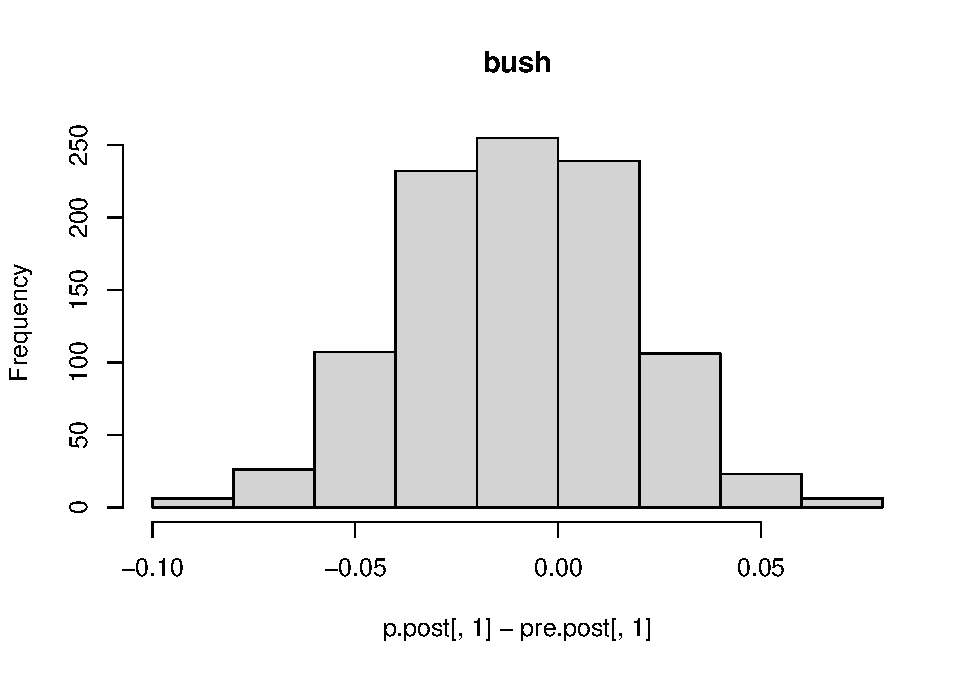
\includegraphics{_main_files/figure-latex/unnamed-chunk-30-1.pdf}

\begin{Shaded}
\begin{Highlighting}[]
   \FunctionTok{table}\NormalTok{((p.post[,}\DecValTok{1}\NormalTok{]}\SpecialCharTok{{-}}\NormalTok{pre.post[,}\DecValTok{1}\NormalTok{])}\SpecialCharTok{\textgreater{}}\DecValTok{0}\NormalTok{) }\DocumentationTok{\#\# 0.355\% supported bush post debate.}
\end{Highlighting}
\end{Shaded}

\begin{verbatim}
## 
## FALSE  TRUE 
##   641   359
\end{verbatim}

\begin{Shaded}
\begin{Highlighting}[]
\NormalTok{ pre.post2}\OtherTok{\textless{}{-}}\FunctionTok{apply}\NormalTok{(theta,}\DecValTok{1}\NormalTok{, }\ControlFlowTok{function}\NormalTok{(x) }\FunctionTok{ddirichlet}\NormalTok{(x,}\FunctionTok{as.numeric}\NormalTok{(debate[}\DecValTok{1}\NormalTok{,}\DecValTok{2}\SpecialCharTok{:}\DecValTok{4}\NormalTok{])))}
\NormalTok{ post.post2}\OtherTok{\textless{}{-}}\FunctionTok{apply}\NormalTok{(theta,}\DecValTok{1}\NormalTok{, }\ControlFlowTok{function}\NormalTok{(x) }\FunctionTok{ddirichlet}\NormalTok{(x,}\FunctionTok{as.numeric}\NormalTok{(debate[}\DecValTok{2}\NormalTok{,}\DecValTok{2}\SpecialCharTok{:}\DecValTok{4}\NormalTok{])))}
 
  \FunctionTok{plot}\NormalTok{(theta[,}\DecValTok{1}\NormalTok{],pre.post2,}\AttributeTok{col=}\StringTok{\textquotesingle{}blue\textquotesingle{}}\NormalTok{,}\AttributeTok{lty=}\DecValTok{2}\NormalTok{)}
  \FunctionTok{lines}\NormalTok{(theta[,}\DecValTok{1}\NormalTok{],post.post2,}\AttributeTok{col=}\StringTok{\textquotesingle{}red\textquotesingle{}}\NormalTok{)}
\end{Highlighting}
\end{Shaded}

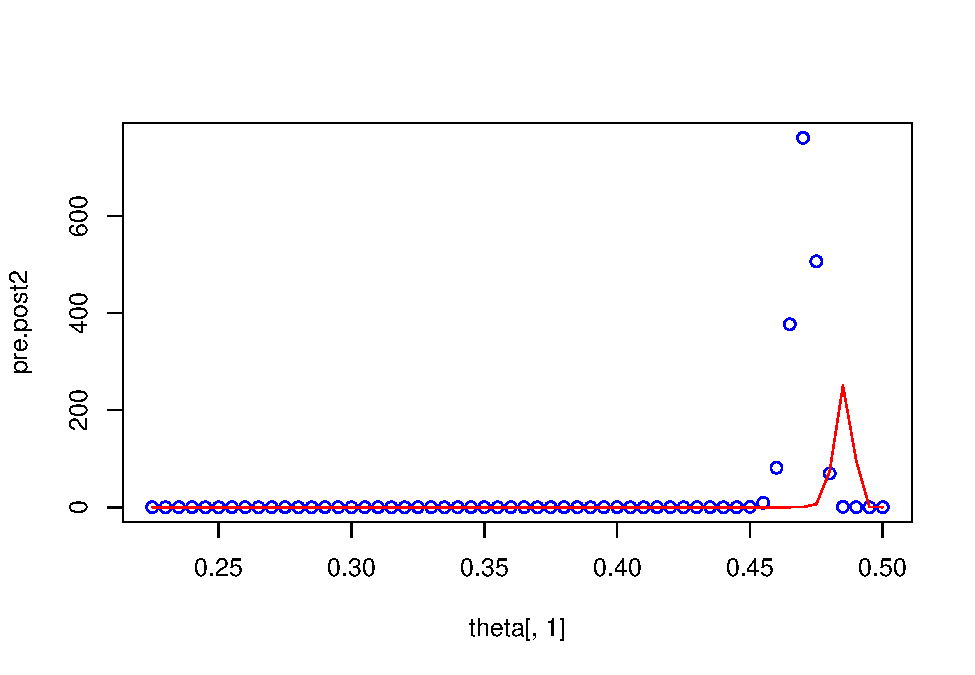
\includegraphics{_main_files/figure-latex/unnamed-chunk-30-2.pdf}

\hypertarget{question-3-1}{%
\section*{Question 3}\label{question-3-1}}
\addcontentsline{toc}{section}{Question 3}

we are given two independent normal random variables with unknown variances and unknown true means.
- (a) Assume a uniform prior on \((\mu_c, \mu_t, log(\sigma_c),log(\sigma_t))\) find the posterior of \(\mu_c\) and \(\mu_t\).

\begin{Shaded}
\begin{Highlighting}[]
\NormalTok{ nc }\OtherTok{=}\DecValTok{32}
\NormalTok{ nt}\OtherTok{=} \DecValTok{36}
\NormalTok{ mc }\OtherTok{=} \FloatTok{1.013}
\NormalTok{ sdc }\OtherTok{=} \FloatTok{0.24}
\NormalTok{ mt }\OtherTok{=} \FloatTok{1.173}
\NormalTok{ sdt }\OtherTok{=} \FloatTok{0.24}
 
 \DocumentationTok{\#\#\# unknow true mean/variances  we only have sample data.}
 \DocumentationTok{\#\# we have two unknowns and need to find the joint posterior distribution.}
 
 \CommentTok{\# the marginal posterior of mc follows a t{-}dist.}
\NormalTok{  mc\_range}\OtherTok{\textless{}{-}}\FunctionTok{c}\NormalTok{(mc}\SpecialCharTok{{-}}\NormalTok{sdc}\SpecialCharTok{/}\FunctionTok{sqrt}\NormalTok{(nc)}\SpecialCharTok{*}\FunctionTok{qt}\NormalTok{(}\FloatTok{0.975}\NormalTok{,}\AttributeTok{df=}\NormalTok{nc}\DecValTok{{-}1}\NormalTok{),mc}\SpecialCharTok{+}\NormalTok{sdc}\SpecialCharTok{/}\FunctionTok{sqrt}\NormalTok{(nc)}\SpecialCharTok{*}\FunctionTok{qt}\NormalTok{(}\FloatTok{0.975}\NormalTok{,}\AttributeTok{df=}\NormalTok{nc}\DecValTok{{-}1}\NormalTok{))}
\NormalTok{   mt\_range}\OtherTok{\textless{}{-}}\FunctionTok{c}\NormalTok{(mt}\SpecialCharTok{{-}}\NormalTok{sdt}\SpecialCharTok{/}\FunctionTok{sqrt}\NormalTok{(nt)}\SpecialCharTok{*}\FunctionTok{qt}\NormalTok{(}\FloatTok{0.975}\NormalTok{,}\AttributeTok{df=}\NormalTok{nt}\DecValTok{{-}1}\NormalTok{),mt}\SpecialCharTok{+}\NormalTok{sdt}\SpecialCharTok{/}\FunctionTok{sqrt}\NormalTok{(nt)}\SpecialCharTok{*}\FunctionTok{qt}\NormalTok{(}\FloatTok{0.975}\NormalTok{,}\AttributeTok{df=}\NormalTok{nt}\DecValTok{{-}1}\NormalTok{))}

\DocumentationTok{\#\# to sample from the posterior we use 3.5 and 3.3 equations}
\NormalTok{   posterior\_sample}\OtherTok{\textless{}{-}}\ControlFlowTok{function}\NormalTok{( }\AttributeTok{mc=}\DecValTok{1}\NormalTok{, }\AttributeTok{sdc=}\DecValTok{1}\NormalTok{, }\AttributeTok{nc=}\DecValTok{10}\NormalTok{)\{}
\NormalTok{   invx2}\OtherTok{\textless{}{-}}\NormalTok{((nc}\DecValTok{{-}1}\NormalTok{)}\SpecialCharTok{*}\NormalTok{sdc}\SpecialCharTok{\^{}}\DecValTok{2}\NormalTok{)}\SpecialCharTok{/}\FunctionTok{rchisq}\NormalTok{(}\DecValTok{1}\NormalTok{,nc}\DecValTok{{-}1}\NormalTok{)}
\NormalTok{    post.mu}\OtherTok{\textless{}{-}}\FunctionTok{rnorm}\NormalTok{(}\DecValTok{1}\NormalTok{,}\AttributeTok{mean=}\NormalTok{mc,}\AttributeTok{sd=}\FunctionTok{sqrt}\NormalTok{(invx2}\SpecialCharTok{/}\NormalTok{nc))}
    \FunctionTok{return}\NormalTok{(post.mu)}
\NormalTok{   \}}
\NormalTok{   post\_mc}\OtherTok{\textless{}{-}}\FunctionTok{sapply}\NormalTok{(}\DecValTok{1}\SpecialCharTok{:}\DecValTok{1000}\NormalTok{,}\ControlFlowTok{function}\NormalTok{(x) }\FunctionTok{posterior\_sample}\NormalTok{(}\AttributeTok{mc=}\NormalTok{mc,}\AttributeTok{sdc=}\NormalTok{sdc,}\AttributeTok{nc=}\NormalTok{nc))}
    \FunctionTok{hist}\NormalTok{(post\_mc,}\AttributeTok{main=}\StringTok{\textquotesingle{}posterior marginal control\textquotesingle{}}\NormalTok{)}
\end{Highlighting}
\end{Shaded}

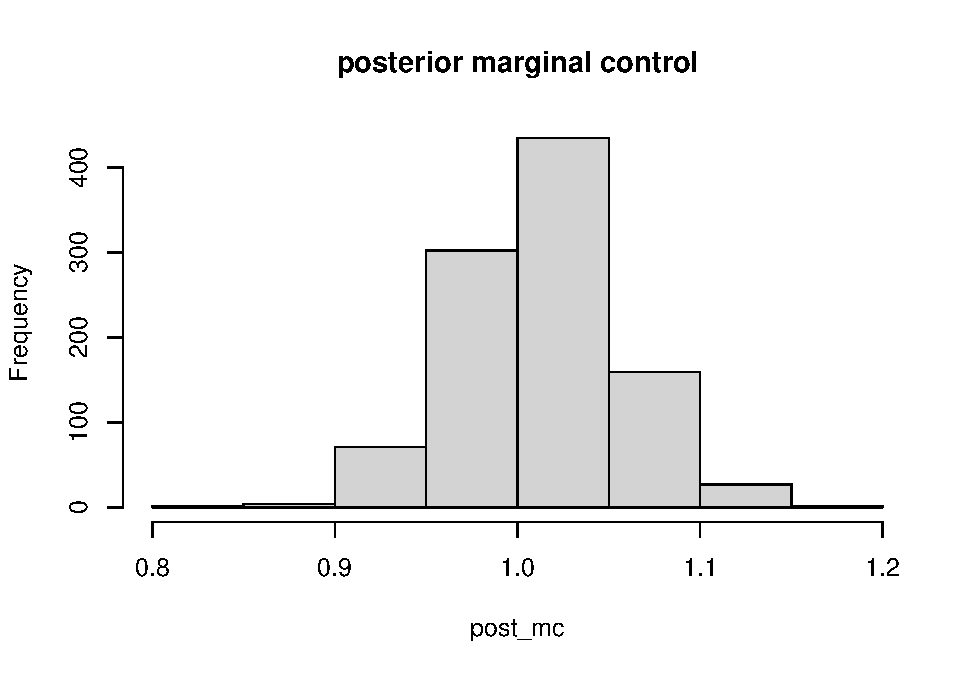
\includegraphics{_main_files/figure-latex/unnamed-chunk-31-1.pdf}

\begin{Shaded}
\begin{Highlighting}[]
\NormalTok{    post\_mt}\OtherTok{\textless{}{-}}\FunctionTok{sapply}\NormalTok{(}\DecValTok{1}\SpecialCharTok{:}\DecValTok{1000}\NormalTok{,}\ControlFlowTok{function}\NormalTok{(x) }\FunctionTok{posterior\_sample}\NormalTok{(}\AttributeTok{mc=}\NormalTok{mt,}\AttributeTok{sdc=}\NormalTok{sdt,}\AttributeTok{nc=}\NormalTok{nt))}
     \FunctionTok{hist}\NormalTok{(post\_mt,}\AttributeTok{main=}\StringTok{\textquotesingle{}posterior marginal treat\textquotesingle{}}\NormalTok{)}
\end{Highlighting}
\end{Shaded}

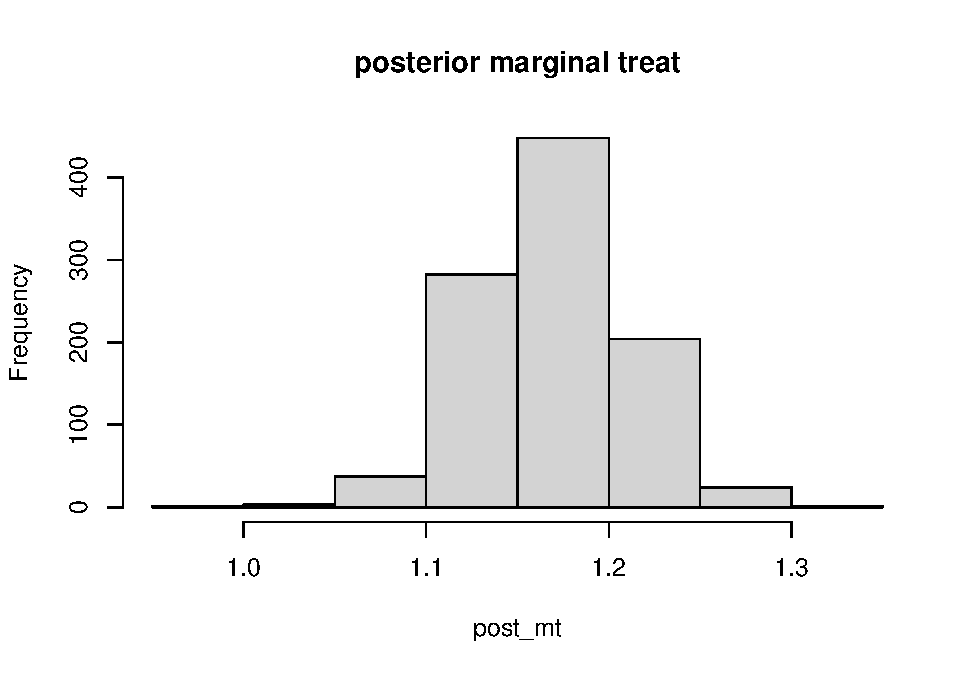
\includegraphics{_main_files/figure-latex/unnamed-chunk-31-2.pdf}

\begin{Shaded}
\begin{Highlighting}[]
    \FunctionTok{message}\NormalTok{(}\StringTok{"95\% posterior margin control:"}\NormalTok{, }\FunctionTok{round}\NormalTok{(mc\_range[}\DecValTok{1}\NormalTok{],}\DecValTok{2}\NormalTok{),}\StringTok{" "}\NormalTok{,}\FunctionTok{round}\NormalTok{(mc\_range[}\DecValTok{2}\NormalTok{],}\DecValTok{2}\NormalTok{)) }
\end{Highlighting}
\end{Shaded}

\begin{verbatim}
## 95% posterior margin control:0.93 1.1
\end{verbatim}

\begin{Shaded}
\begin{Highlighting}[]
        \FunctionTok{message}\NormalTok{(}\StringTok{"95\% posterior margin control:"}\NormalTok{, }\FunctionTok{round}\NormalTok{(mt\_range[}\DecValTok{1}\NormalTok{],}\DecValTok{2}\NormalTok{),}\StringTok{" "}\NormalTok{,}\FunctionTok{round}\NormalTok{(mt\_range[}\DecValTok{2}\NormalTok{],}\DecValTok{2}\NormalTok{)) }
\end{Highlighting}
\end{Shaded}

\begin{verbatim}
## 95% posterior margin control:1.09 1.25
\end{verbatim}

\begin{Shaded}
\begin{Highlighting}[]
        \FunctionTok{quantile}\NormalTok{(post\_mc,}\FunctionTok{c}\NormalTok{(}\FloatTok{0.025}\NormalTok{,}\FloatTok{0.975}\NormalTok{))}
\end{Highlighting}
\end{Shaded}

\begin{verbatim}
##      2.5%     97.5% 
## 0.9324065 1.0975105
\end{verbatim}

\begin{Shaded}
\begin{Highlighting}[]
        \FunctionTok{quantile}\NormalTok{(post\_mt,}\FunctionTok{c}\NormalTok{(}\FloatTok{0.025}\NormalTok{,}\FloatTok{0.975}\NormalTok{))}
\end{Highlighting}
\end{Shaded}

\begin{verbatim}
##     2.5%    97.5% 
## 1.092578 1.250800
\end{verbatim}

\begin{itemize}
\item
  \begin{enumerate}
  \def\labelenumi{(\alph{enumi})}
  \setcounter{enumi}{1}
  \tightlist
  \item
    what is \(\mu_t - \mu_c\)
  \end{enumerate}
\end{itemize}

The posterior interval (central) of the differences between 2 independent t-distributoins is 0.16 (0.04, 0.28), which closely matches the posterior simulation interval (0.0338, 0.281). Here since both are independent we use \(X-Y\sim N(\mu_x-\mu_y, sd_x+sd_y)\) as the sampling distribution.

\begin{Shaded}
\begin{Highlighting}[]
 \FunctionTok{hist}\NormalTok{(post\_mt}\SpecialCharTok{{-}}\NormalTok{post\_mc, }\AttributeTok{main =} \StringTok{\textquotesingle{} Difference between sampled posteriors\textquotesingle{}}\NormalTok{)}
\end{Highlighting}
\end{Shaded}

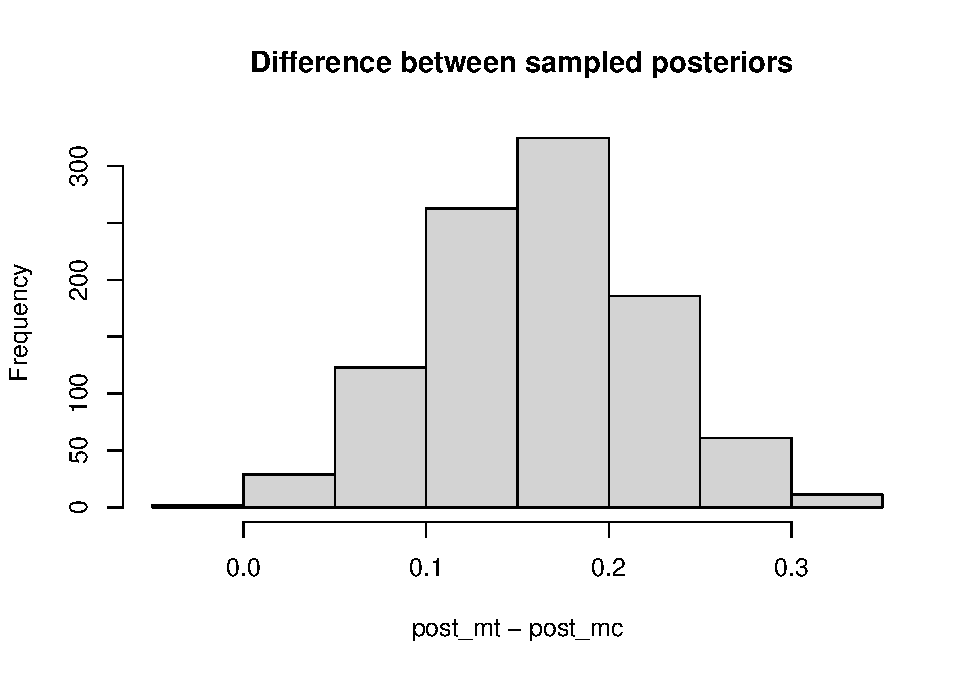
\includegraphics{_main_files/figure-latex/unnamed-chunk-32-1.pdf}

\begin{Shaded}
\begin{Highlighting}[]
         \FunctionTok{quantile}\NormalTok{(post\_mt}\SpecialCharTok{{-}}\NormalTok{post\_mc,}\FunctionTok{c}\NormalTok{(}\FloatTok{0.025}\NormalTok{,}\FloatTok{0.975}\NormalTok{))}
\end{Highlighting}
\end{Shaded}

\begin{verbatim}
##       2.5%      97.5% 
## 0.04929078 0.28347800
\end{verbatim}

\begin{Shaded}
\begin{Highlighting}[]
  \DocumentationTok{\#\# diff}
\NormalTok{         post\_diff}\OtherTok{\textless{}{-}}\FunctionTok{sapply}\NormalTok{(}\DecValTok{1}\SpecialCharTok{:}\DecValTok{1000}\NormalTok{,}\ControlFlowTok{function}\NormalTok{(x) }\FunctionTok{posterior\_sample}\NormalTok{(}\AttributeTok{mc=}\NormalTok{mt}\SpecialCharTok{{-}}\NormalTok{mc,}\AttributeTok{sdc=}\NormalTok{sdt}\SpecialCharTok{+}\NormalTok{sdc,}\AttributeTok{nc=}\NormalTok{nt}\SpecialCharTok{+}\NormalTok{nc))}
    \FunctionTok{hist}\NormalTok{(post\_diff, }\AttributeTok{main=}\StringTok{\textquotesingle{}simulated difference\textquotesingle{}}\NormalTok{)}
\end{Highlighting}
\end{Shaded}

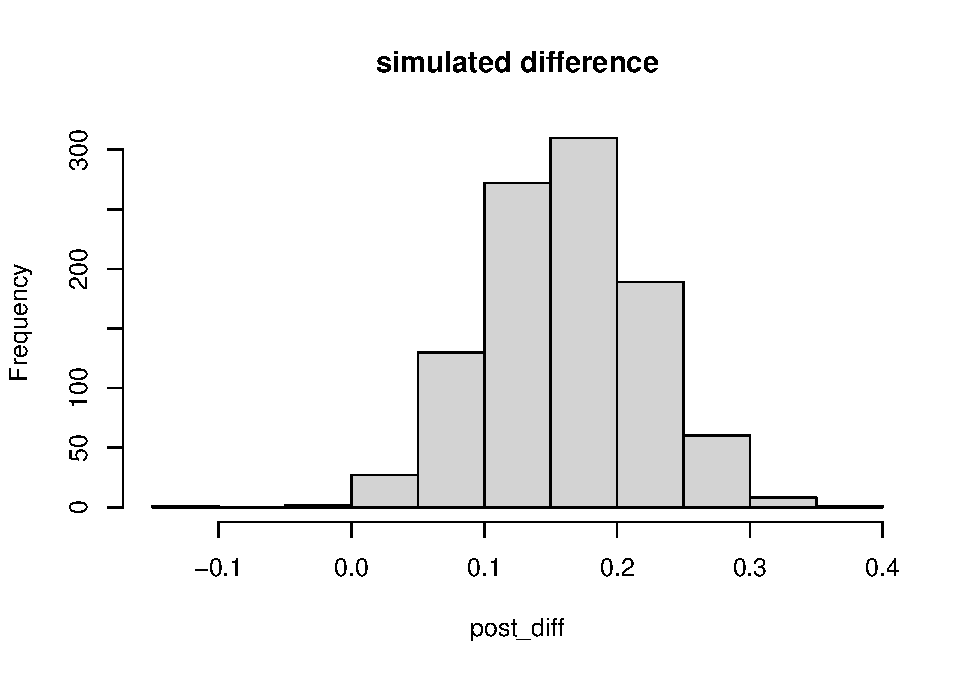
\includegraphics{_main_files/figure-latex/unnamed-chunk-32-2.pdf}

\begin{Shaded}
\begin{Highlighting}[]
             \FunctionTok{quantile}\NormalTok{(post\_diff,}\FunctionTok{c}\NormalTok{(}\FloatTok{0.025}\NormalTok{,}\FloatTok{0.975}\NormalTok{))}
\end{Highlighting}
\end{Shaded}

\begin{verbatim}
##       2.5%      97.5% 
## 0.03981079 0.27082799
\end{verbatim}

\begin{Shaded}
\begin{Highlighting}[]
  \DocumentationTok{\#\# theoretical (two independent t distributions)}
\NormalTok{  md }\OtherTok{=}\NormalTok{ mt}\SpecialCharTok{{-}}\NormalTok{mc}
\NormalTok{  sdd }\OtherTok{=}\NormalTok{ sdt}\SpecialCharTok{+}\NormalTok{sdc}
\NormalTok{  nd }\OtherTok{=}\NormalTok{ nt}\SpecialCharTok{+}\NormalTok{nc}
\NormalTok{  d\_range}\OtherTok{\textless{}{-}}\FunctionTok{c}\NormalTok{(md}\SpecialCharTok{{-}}\NormalTok{sdd}\SpecialCharTok{/}\FunctionTok{sqrt}\NormalTok{(nd)}\SpecialCharTok{*}\FunctionTok{qt}\NormalTok{(}\FloatTok{0.975}\NormalTok{,}\AttributeTok{df=}\NormalTok{nd}\DecValTok{{-}1}\NormalTok{),md}\SpecialCharTok{+}\NormalTok{sdd}\SpecialCharTok{/}\FunctionTok{sqrt}\NormalTok{(nd)}\SpecialCharTok{*}\FunctionTok{qt}\NormalTok{(}\FloatTok{0.975}\NormalTok{,}\AttributeTok{df=}\NormalTok{nd}\DecValTok{{-}1}\NormalTok{))}
  \FunctionTok{print}\NormalTok{(d\_range)}
\end{Highlighting}
\end{Shaded}

\begin{verbatim}
## [1] 0.04381525 0.27618475
\end{verbatim}

\hypertarget{question-4-independent-binomial}{%
\section*{Question 4 (independent binomial)}\label{question-4-independent-binomial}}
\addcontentsline{toc}{section}{Question 4 (independent binomial)}

so using the multinomial is not correct because we do not have k outcomes, instead we have 2 independent binomial processes (as the question states!) so we modeled the independent likelihoods, which is a product of independent beta distributions.

\(p(p_0,p_1) \propto p(x| p_0,p_1)p(p_0,p_1) = p_0^{38.5}(1-p_0)^{634.5}p_1^{21.5}(1-p_1)^{657.5}\)

\begin{Shaded}
\begin{Highlighting}[]
\NormalTok{p0}\OtherTok{=} \FunctionTok{seq}\NormalTok{(}\FloatTok{0.01}\NormalTok{,}\FloatTok{0.99}\NormalTok{,}\AttributeTok{by=}\FloatTok{0.01}\NormalTok{)}
\NormalTok{p1}\OtherTok{=} \FunctionTok{seq}\NormalTok{(}\FloatTok{0.01}\NormalTok{,}\FloatTok{0.99}\NormalTok{,}\AttributeTok{by=}\FloatTok{0.01}\NormalTok{)}

\NormalTok{post.bin}\OtherTok{\textless{}{-}}\ControlFlowTok{function}\NormalTok{(p0,p1)\{}
\NormalTok{  pos}\OtherTok{\textless{}{-}}\NormalTok{ p0}\SpecialCharTok{\^{}}\NormalTok{(}\FloatTok{38.5}\NormalTok{)}\SpecialCharTok{*}\NormalTok{(}\DecValTok{1}\SpecialCharTok{{-}}\NormalTok{p0)}\SpecialCharTok{\^{}}\NormalTok{(}\FloatTok{634.5}\NormalTok{)}\SpecialCharTok{*}\NormalTok{p1}\SpecialCharTok{\^{}}\NormalTok{(}\FloatTok{21.5}\NormalTok{)}\SpecialCharTok{*}\NormalTok{(}\DecValTok{1}\SpecialCharTok{{-}}\NormalTok{p1)}\SpecialCharTok{\^{}}\NormalTok{(}\FloatTok{657.5}\NormalTok{)}
  \FunctionTok{return}\NormalTok{(pos)}
\NormalTok{\}}
\NormalTok{ posts}\OtherTok{\textless{}{-}}\ConstantTok{NULL}
 
\NormalTok{p0p1}\OtherTok{\textless{}{-}} \FunctionTok{expand.grid}\NormalTok{(p0, p1)}

\ControlFlowTok{for}\NormalTok{(i }\ControlFlowTok{in} \DecValTok{1}\SpecialCharTok{:}\FunctionTok{nrow}\NormalTok{(p0p1))\{}
\NormalTok{  posts[i]}\OtherTok{\textless{}{-}}\FunctionTok{post.bin}\NormalTok{(p0p1[i,}\StringTok{"Var1"}\NormalTok{],p0p1[i,}\StringTok{"Var2"}\NormalTok{]) }
\NormalTok{\}}

 \FunctionTok{ggplot}\NormalTok{(p0p1)}\SpecialCharTok{+}
 \FunctionTok{geom\_contour}\NormalTok{(}\AttributeTok{mapping =} \FunctionTok{aes}\NormalTok{(}\AttributeTok{x =}\NormalTok{ Var1, }\AttributeTok{y =}\NormalTok{ Var2, }\AttributeTok{z =}\NormalTok{ posts), }\AttributeTok{bins =} \DecValTok{20}\NormalTok{)}
\end{Highlighting}
\end{Shaded}

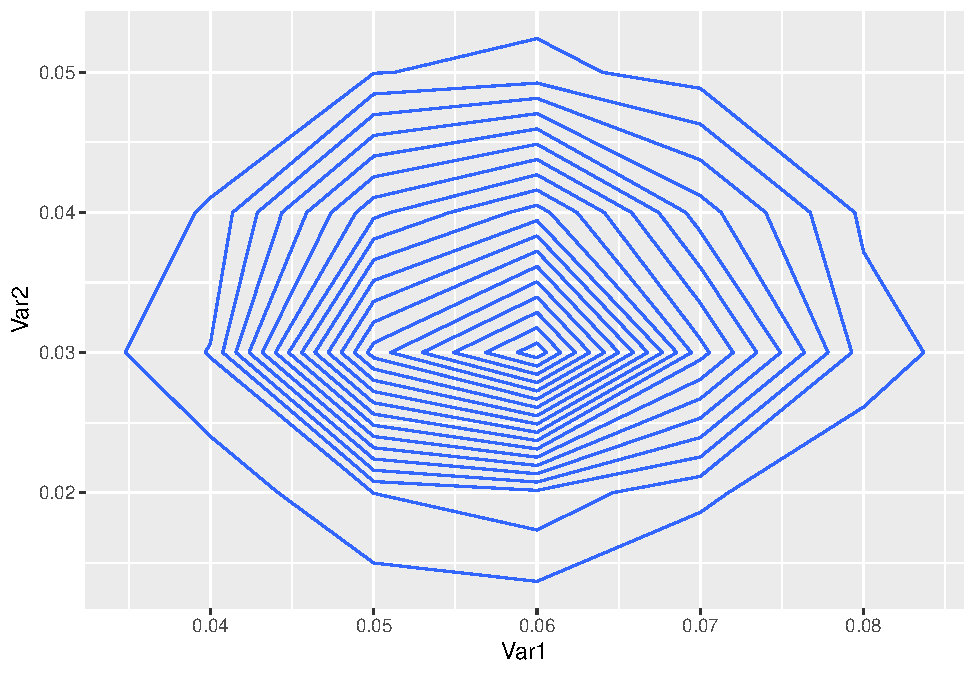
\includegraphics{_main_files/figure-latex/unnamed-chunk-33-1.pdf}

\begin{itemize}
\item
  \begin{enumerate}
  \def\labelenumi{(\alph{enumi})}
  \setcounter{enumi}{1}
  \tightlist
  \item
    summarize the odds ratio
    Note that using a 2x2 table the OR is 0.54 and the independent binomials do approximate well.
  \end{enumerate}
\end{itemize}

\begin{Shaded}
\begin{Highlighting}[]
\NormalTok{b1}\OtherTok{\textless{}{-}}\FunctionTok{sapply}\NormalTok{(p0,}\ControlFlowTok{function}\NormalTok{(x) }\FunctionTok{pbeta}\NormalTok{(x,}\FloatTok{38.5}\NormalTok{,}\FloatTok{634.5}\NormalTok{))}
\NormalTok{ post.control}\OtherTok{\textless{}{-}}\FunctionTok{rbeta}\NormalTok{(}\DecValTok{1000}\NormalTok{, }\FloatTok{38.5}\NormalTok{,}\FloatTok{634.5}\NormalTok{)}
\NormalTok{  post.treat}\OtherTok{\textless{}{-}}\FunctionTok{rbeta}\NormalTok{(}\DecValTok{1000}\NormalTok{, }\FloatTok{21.5}\NormalTok{,}\FloatTok{657.5}\NormalTok{)}

\NormalTok{  or}\OtherTok{\textless{}{-}}\NormalTok{(post.treat}\SpecialCharTok{/}\NormalTok{(}\DecValTok{1}\SpecialCharTok{{-}}\NormalTok{post.treat))}\SpecialCharTok{/}\NormalTok{(post.control}\SpecialCharTok{/}\NormalTok{(}\DecValTok{1}\SpecialCharTok{{-}}\NormalTok{post.control))}
  \FunctionTok{hist}\NormalTok{(or,}\AttributeTok{main=}\StringTok{\textquotesingle{}treatment odds empriical posterior\textquotesingle{}}\NormalTok{)}
\end{Highlighting}
\end{Shaded}

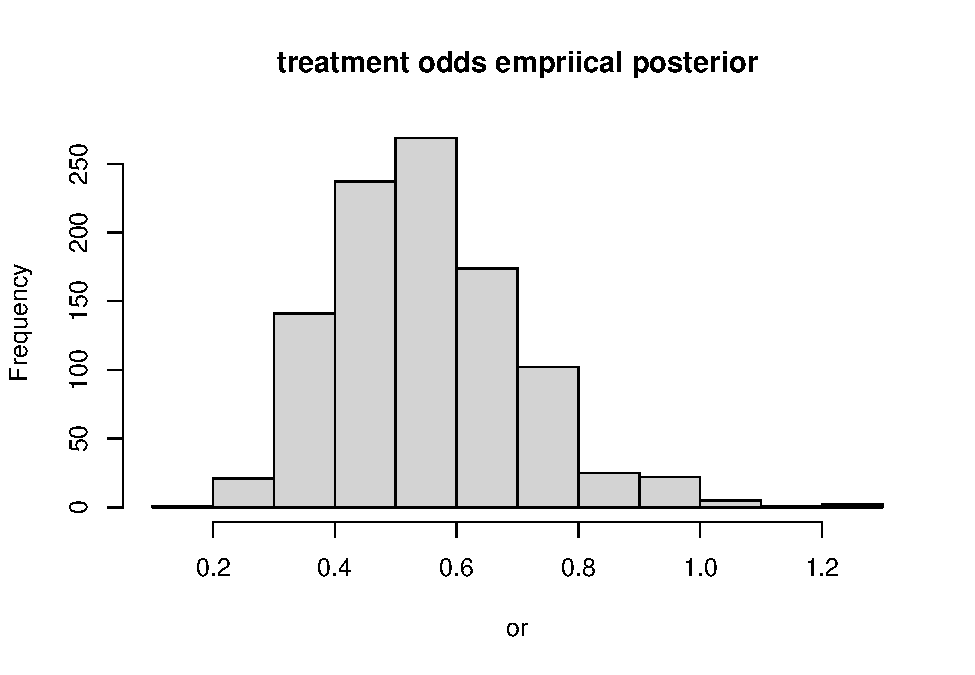
\includegraphics{_main_files/figure-latex/unnamed-chunk-34-1.pdf}

\begin{Shaded}
\begin{Highlighting}[]
  \FunctionTok{summary}\NormalTok{(or)}
\end{Highlighting}
\end{Shaded}

\begin{verbatim}
##    Min. 1st Qu.  Median    Mean 3rd Qu.    Max. 
##  0.2200  0.4435  0.5295  0.5484  0.6429  1.1370
\end{verbatim}

\begin{Shaded}
\begin{Highlighting}[]
  \FunctionTok{message}\NormalTok{(}\StringTok{"the empricial OR: "}\NormalTok{, }\FunctionTok{round}\NormalTok{((}\DecValTok{22}\SpecialCharTok{*}\DecValTok{635}\NormalTok{)}\SpecialCharTok{/}\NormalTok{(}\DecValTok{39}\SpecialCharTok{*}\DecValTok{658}\NormalTok{),}\DecValTok{2}\NormalTok{))}
\end{Highlighting}
\end{Shaded}

\begin{verbatim}
## the empricial OR: 0.54
\end{verbatim}

\begin{itemize}
\item
  \begin{enumerate}
  \def\labelenumi{(\alph{enumi})}
  \setcounter{enumi}{2}
  \tightlist
  \item
    the sensitivity of the noninformative prior density
    If we use the prior Beta(1,1) as the uniform prior we do see marginal changes to the posterior mean 0.5639.
  \end{enumerate}
\end{itemize}

\begin{Shaded}
\begin{Highlighting}[]
\NormalTok{b1}\OtherTok{\textless{}{-}}\FunctionTok{sapply}\NormalTok{(p0,}\ControlFlowTok{function}\NormalTok{(x) }\FunctionTok{pbeta}\NormalTok{(x,}\FloatTok{39.5}\NormalTok{,}\FloatTok{635.5}\NormalTok{))}
\NormalTok{ post.control}\OtherTok{\textless{}{-}}\FunctionTok{rbeta}\NormalTok{(}\DecValTok{1000}\NormalTok{, }\FloatTok{39.5}\NormalTok{,}\FloatTok{635.5}\NormalTok{)}
\NormalTok{  post.treat}\OtherTok{\textless{}{-}}\FunctionTok{rbeta}\NormalTok{(}\DecValTok{1000}\NormalTok{, }\FloatTok{22.5}\NormalTok{,}\FloatTok{658.5}\NormalTok{)}

\NormalTok{  or}\OtherTok{\textless{}{-}}\NormalTok{(post.treat}\SpecialCharTok{/}\NormalTok{(}\DecValTok{1}\SpecialCharTok{{-}}\NormalTok{post.treat))}\SpecialCharTok{/}\NormalTok{(post.control}\SpecialCharTok{/}\NormalTok{(}\DecValTok{1}\SpecialCharTok{{-}}\NormalTok{post.control))}
  \FunctionTok{hist}\NormalTok{(or,}\AttributeTok{main=}\StringTok{\textquotesingle{}treatment odds empriical posterior\textquotesingle{}}\NormalTok{)}
\end{Highlighting}
\end{Shaded}

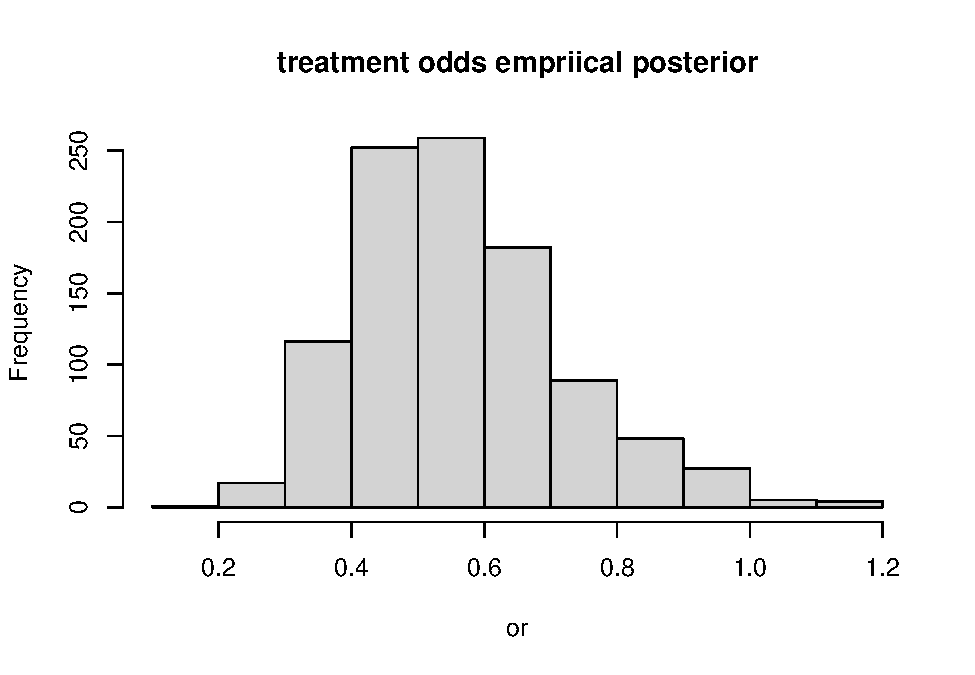
\includegraphics{_main_files/figure-latex/unnamed-chunk-35-1.pdf}

\begin{Shaded}
\begin{Highlighting}[]
  \FunctionTok{summary}\NormalTok{(or)}
\end{Highlighting}
\end{Shaded}

\begin{verbatim}
##    Min. 1st Qu.  Median    Mean 3rd Qu.    Max. 
##  0.2096  0.4648  0.5561  0.5739  0.6627  1.3870
\end{verbatim}

\hypertarget{question-4-dirichlet}{%
\subsection*{Question 4 (dirichlet)}\label{question-4-dirichlet}}
\addcontentsline{toc}{subsection}{Question 4 (dirichlet)}

\begin{itemize}
\tightlist
\item
  (4a) set up a noninformative prior on \((p_0,p_1)\) and obtain posterior simulations. Assume outcomes are independent and binomially distributed. The posterior for probability of death is Diri(39+1, 22+1, 675,681)
\item
  the dirichlet is the event of rolling a 4 sided die, whereas this problem is rolling independent 2 sided die, however the dirichlet does approximate independnet binomial processes well.
\end{itemize}

\begin{Shaded}
\begin{Highlighting}[]
\NormalTok{ nc}\OtherTok{=} \DecValTok{674}
\NormalTok{ dc}\OtherTok{=} \DecValTok{39}
\NormalTok{ nt }\OtherTok{=} \DecValTok{680}
\NormalTok{ dt }\OtherTok{=} \DecValTok{22}

 
 
 \DocumentationTok{\#\# we have two categories Control \textasciitilde{}Bin(p0) and Treat\textasciitilde{}Bin(p1) we use multinomial}
 \DocumentationTok{\#\# non{-}informative prior Diri(a1=1, a2=1)}
 \FunctionTok{library}\NormalTok{(gtools)}
  \DocumentationTok{\#\# p( p0, p1) = Diri( 1,1) noninfom prior}
  \CommentTok{\# p( p0,p1 | y) = Diri(  39+1, 22+1) \#\#  posterior}
 
\NormalTok{ treat.post}\OtherTok{\textless{}{-}}\FunctionTok{rdirichlet}\NormalTok{(}\DecValTok{1000}\NormalTok{, }\FunctionTok{c}\NormalTok{(}\DecValTok{39}\SpecialCharTok{+}\DecValTok{1}\NormalTok{,}\DecValTok{22}\SpecialCharTok{+}\DecValTok{1}\NormalTok{, }\DecValTok{674}\SpecialCharTok{+}\DecValTok{1}\NormalTok{,}\DecValTok{680}\SpecialCharTok{+}\DecValTok{1}\NormalTok{))}
 \FunctionTok{par}\NormalTok{(}\AttributeTok{mfrow=}\FunctionTok{c}\NormalTok{(}\DecValTok{1}\NormalTok{,}\DecValTok{2}\NormalTok{))}
  \FunctionTok{hist}\NormalTok{(treat.post[,}\DecValTok{1}\NormalTok{],}\AttributeTok{main=}\StringTok{"post control"}\NormalTok{)}
  \FunctionTok{hist}\NormalTok{(treat.post[,}\DecValTok{2}\NormalTok{],}\AttributeTok{main=}\StringTok{\textquotesingle{}post treat\textquotesingle{}}\NormalTok{)}
\end{Highlighting}
\end{Shaded}

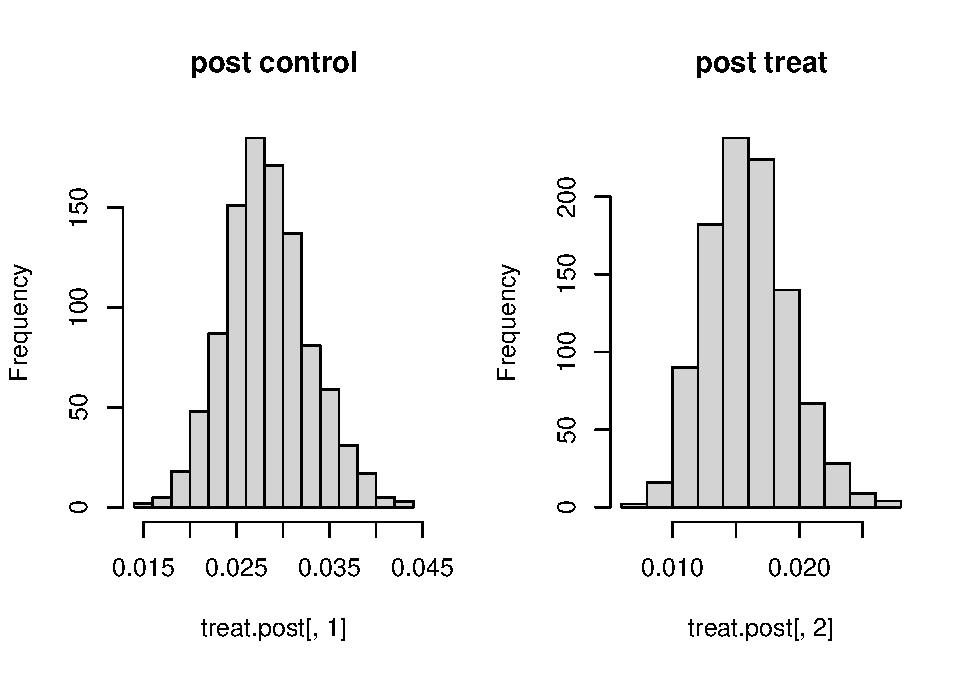
\includegraphics{_main_files/figure-latex/unnamed-chunk-36-1.pdf}

\begin{itemize}
\tightlist
\item
  (4b) The posterior odds has a mean of 0.58 using non-informative prior. Using the empirical odds ratio we see the odds of death is 0.546 comparing treatment to controls.
\end{itemize}

\begin{Shaded}
\begin{Highlighting}[]
 \DocumentationTok{\#\# data table}
\NormalTok{ dd}\OtherTok{\textless{}{-}}\FunctionTok{data.frame}\NormalTok{(}\AttributeTok{none=}\FunctionTok{c}\NormalTok{(}\DecValTok{674{-}39}\NormalTok{,}\DecValTok{680{-}22}\NormalTok{),}\AttributeTok{outcome=}\FunctionTok{c}\NormalTok{(}\DecValTok{39}\NormalTok{,}\DecValTok{22}\NormalTok{),}\AttributeTok{row.names=}\FunctionTok{c}\NormalTok{(}\StringTok{\textquotesingle{}unexp\textquotesingle{}}\NormalTok{,}\StringTok{\textquotesingle{}exp\textquotesingle{}}\NormalTok{))}
 \FunctionTok{library}\NormalTok{(epitools)}
 \FunctionTok{oddsratio}\NormalTok{(}\FunctionTok{as.matrix}\NormalTok{(dd))}\SpecialCharTok{$}\NormalTok{measure}
\end{Highlighting}
\end{Shaded}

\begin{verbatim}
##                         NA
## odds ratio with 95% C.I.  estimate     lower     upper
##                    unexp 1.0000000        NA        NA
##                    exp   0.5463245 0.3147296 0.9249902
\end{verbatim}

\begin{Shaded}
\begin{Highlighting}[]
  \DocumentationTok{\#\# b}
\NormalTok{  or}\OtherTok{\textless{}{-}}\NormalTok{(treat.post[,}\DecValTok{2}\NormalTok{]}\SpecialCharTok{/}\NormalTok{(}\DecValTok{1}\SpecialCharTok{{-}}\NormalTok{treat.post[,}\DecValTok{2}\NormalTok{]))}\SpecialCharTok{/}\NormalTok{(treat.post[,}\DecValTok{1}\NormalTok{]}\SpecialCharTok{/}\NormalTok{(}\DecValTok{1}\SpecialCharTok{{-}}\NormalTok{treat.post[,}\DecValTok{1}\NormalTok{]))}
\FunctionTok{summary}\NormalTok{(or)}
\end{Highlighting}
\end{Shaded}

\begin{verbatim}
##    Min. 1st Qu.  Median    Mean 3rd Qu.    Max. 
##  0.2176  0.4582  0.5586  0.5792  0.6732  1.1931
\end{verbatim}

\begin{Shaded}
\begin{Highlighting}[]
  \FunctionTok{hist}\NormalTok{(or,}\AttributeTok{main=}\StringTok{\textquotesingle{}treatment odds\textquotesingle{}}\NormalTok{)}
\end{Highlighting}
\end{Shaded}

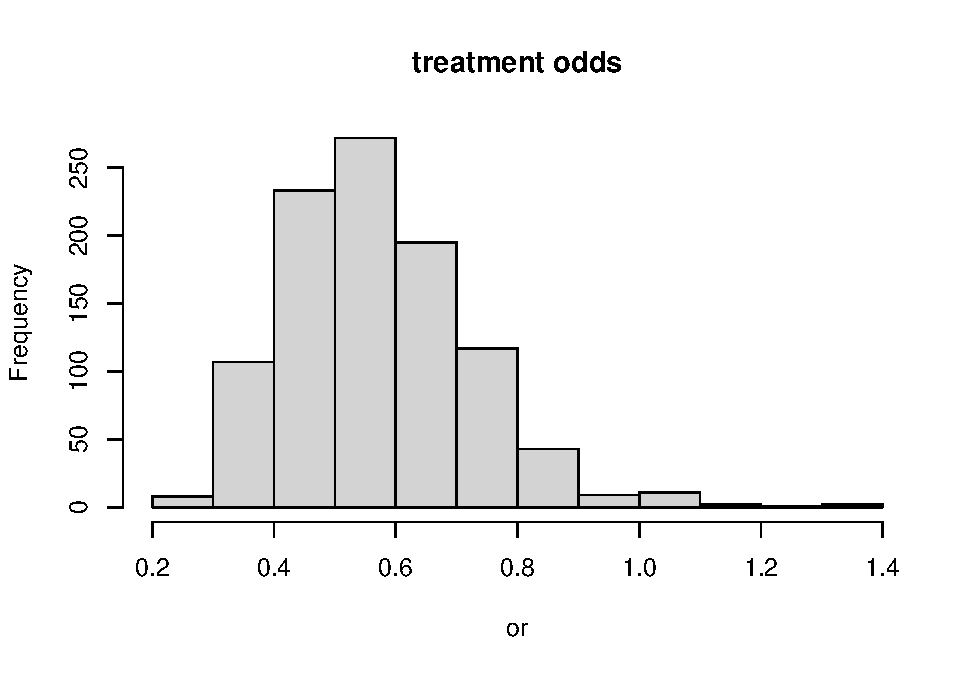
\includegraphics{_main_files/figure-latex/unnamed-chunk-37-1.pdf}

\begin{itemize}
\tightlist
\item
  (4c) showing the improper prior (a=0), the posterior odds is 0.5793 which is very robust and similar to the noninformative. Using the emprical prior that sets the prior hyperparameters to the cohort expected number of deaths \((39/674)*Total = 79\), and \((22/658)*Total = 45\) and a prior cohort size of 677 =(674+680)/2, yields a similar posterior mean of approximately 0.57 for the odds ratio. Hence the posterior is robust to the choice of prior but does not match well with the empirical non-parametric odds.
\end{itemize}

\begin{Shaded}
\begin{Highlighting}[]
\NormalTok{ treat.post}\OtherTok{\textless{}{-}}\FunctionTok{rdirichlet}\NormalTok{(}\DecValTok{1000}\NormalTok{, }\FunctionTok{c}\NormalTok{(}\DecValTok{39}\NormalTok{,}\DecValTok{22}\NormalTok{,}\DecValTok{674}\NormalTok{,}\DecValTok{680}\NormalTok{))}
 
  
  \DocumentationTok{\#\# b}
\NormalTok{  or}\OtherTok{\textless{}{-}}\NormalTok{(treat.post[,}\DecValTok{2}\NormalTok{]}\SpecialCharTok{/}\NormalTok{(}\DecValTok{1}\SpecialCharTok{{-}}\NormalTok{treat.post[,}\DecValTok{2}\NormalTok{]))}\SpecialCharTok{/}\NormalTok{(treat.post[,}\DecValTok{1}\NormalTok{]}\SpecialCharTok{/}\NormalTok{(}\DecValTok{1}\SpecialCharTok{{-}}\NormalTok{treat.post[,}\DecValTok{1}\NormalTok{]))}
  \FunctionTok{hist}\NormalTok{(or,}\AttributeTok{main=}\StringTok{\textquotesingle{}treatment odds \textquotesingle{}}\NormalTok{)}
\end{Highlighting}
\end{Shaded}

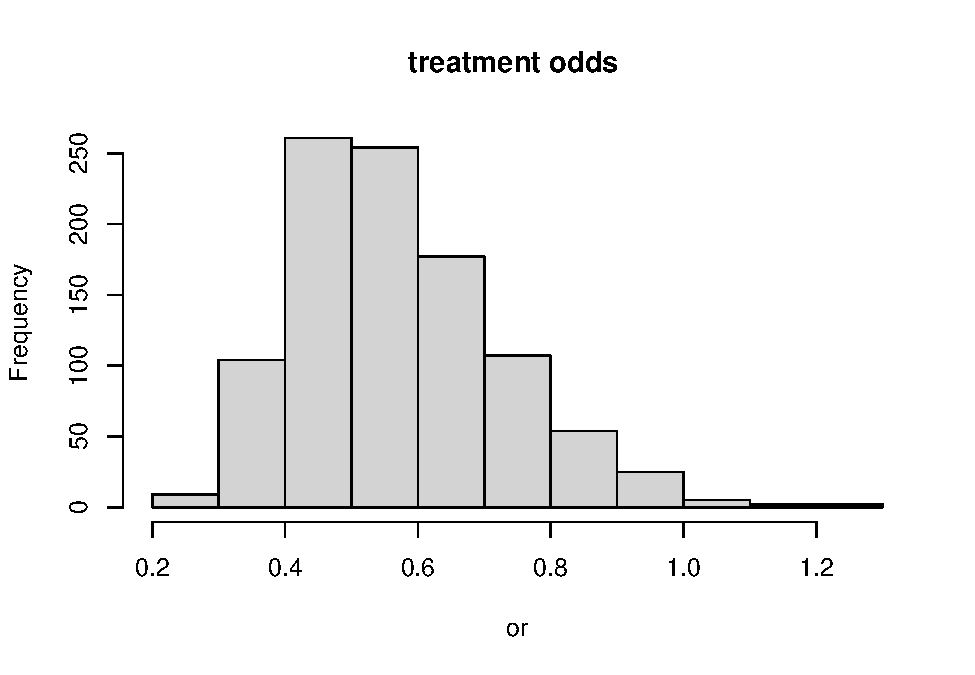
\includegraphics{_main_files/figure-latex/unnamed-chunk-38-1.pdf}

\begin{Shaded}
\begin{Highlighting}[]
  \FunctionTok{summary}\NormalTok{(or)}
\end{Highlighting}
\end{Shaded}

\begin{verbatim}
##    Min. 1st Qu.  Median    Mean 3rd Qu.    Max. 
##  0.1977  0.4579  0.5499  0.5686  0.6551  1.3035
\end{verbatim}

\begin{Shaded}
\begin{Highlighting}[]
  \DocumentationTok{\#\# empirical}
  \CommentTok{\# control = (39/674)*1354 = 78.34718}
  \CommentTok{\# treat = (22/658)*1354 = 45.27052}
\NormalTok{  treat.post}\OtherTok{\textless{}{-}}\FunctionTok{rdirichlet}\NormalTok{(}\DecValTok{1000}\NormalTok{, }\FunctionTok{c}\NormalTok{(}\DecValTok{39}\SpecialCharTok{+}\DecValTok{79}\NormalTok{,}\DecValTok{22}\SpecialCharTok{+}\DecValTok{46}\NormalTok{,}\DecValTok{674}\SpecialCharTok{+}\DecValTok{677}\NormalTok{,}\DecValTok{680}\SpecialCharTok{+}\DecValTok{677}\NormalTok{))}
 
  
  \DocumentationTok{\#\# b}
\NormalTok{  or}\OtherTok{\textless{}{-}}\NormalTok{(treat.post[,}\DecValTok{2}\NormalTok{]}\SpecialCharTok{/}\NormalTok{(}\DecValTok{1}\SpecialCharTok{{-}}\NormalTok{treat.post[,}\DecValTok{2}\NormalTok{]))}\SpecialCharTok{/}\NormalTok{(treat.post[,}\DecValTok{1}\NormalTok{]}\SpecialCharTok{/}\NormalTok{(}\DecValTok{1}\SpecialCharTok{{-}}\NormalTok{treat.post[,}\DecValTok{1}\NormalTok{]))}
  \FunctionTok{hist}\NormalTok{(or,}\AttributeTok{main=}\StringTok{\textquotesingle{}treatment odds empriical posterior\textquotesingle{}}\NormalTok{)}
\end{Highlighting}
\end{Shaded}

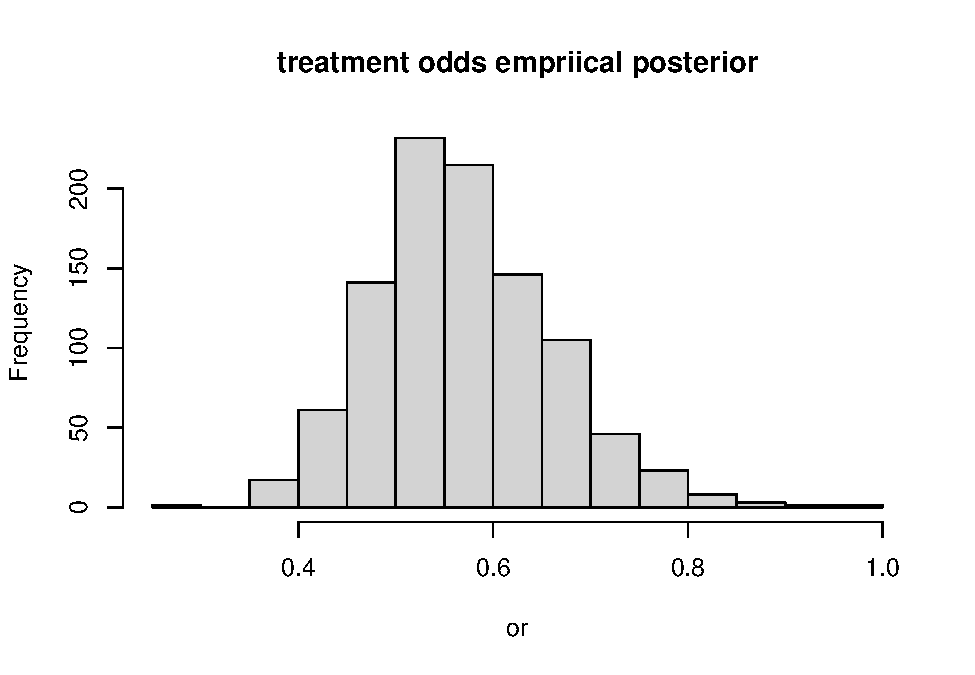
\includegraphics{_main_files/figure-latex/unnamed-chunk-38-2.pdf}

\begin{Shaded}
\begin{Highlighting}[]
  \FunctionTok{summary}\NormalTok{(or)}
\end{Highlighting}
\end{Shaded}

\begin{verbatim}
##    Min. 1st Qu.  Median    Mean 3rd Qu.    Max. 
##  0.3436  0.5094  0.5673  0.5746  0.6370  0.9976
\end{verbatim}

\hypertarget{question-5}{%
\section*{Question 5}\label{question-5}}
\addcontentsline{toc}{section}{Question 5}

\begin{itemize}
\item
  \begin{enumerate}
  \def\labelenumi{(\alph{enumi})}
  \tightlist
  \item
    Give the posterior distribution of \(\mu, \sigma^2\) obtained by pretending the observations are exact, unrounded, measurements. we choose a prior for \(\theta \sim Gamma(0.1,0.01)\) which has a mean and variance of 10.4 and 1000. Using a Poisson likelihood, the mean is 10.4 and variance 2.2 from the posterior.
  \end{enumerate}
\end{itemize}

\begin{Shaded}
\begin{Highlighting}[]
\NormalTok{ obs}\OtherTok{=}\FunctionTok{c}\NormalTok{(}\DecValTok{10}\NormalTok{,}\DecValTok{10}\NormalTok{,}\DecValTok{12}\NormalTok{,}\DecValTok{11}\NormalTok{,}\DecValTok{9}\NormalTok{)}
 \DocumentationTok{\#\#\# under the exact model, we can not use a binomial because we do not have a proportion (p0) that we can estimate. we do not have a r.v. for \textquotesingle{}successes\textquotesingle{}.}
 \CommentTok{\# we can use the Poisson distribution }
 \DocumentationTok{\#\# not sure how to use jeffreys prior}
\NormalTok{  a}\OtherTok{=}\FloatTok{0.1}
\NormalTok{  b}\OtherTok{=}\FloatTok{0.01}
\NormalTok{  pois.post}\OtherTok{\textless{}{-}}\FunctionTok{rgamma}\NormalTok{(}\DecValTok{1000}\NormalTok{,a}\SpecialCharTok{+}\DecValTok{5}\SpecialCharTok{*}\FunctionTok{mean}\NormalTok{(obs),b}\SpecialCharTok{+}\DecValTok{5}\NormalTok{)}
  \FunctionTok{hist}\NormalTok{(pois.post,}\AttributeTok{main=}\StringTok{\textquotesingle{}count posterior\textquotesingle{}}\NormalTok{)}
\end{Highlighting}
\end{Shaded}

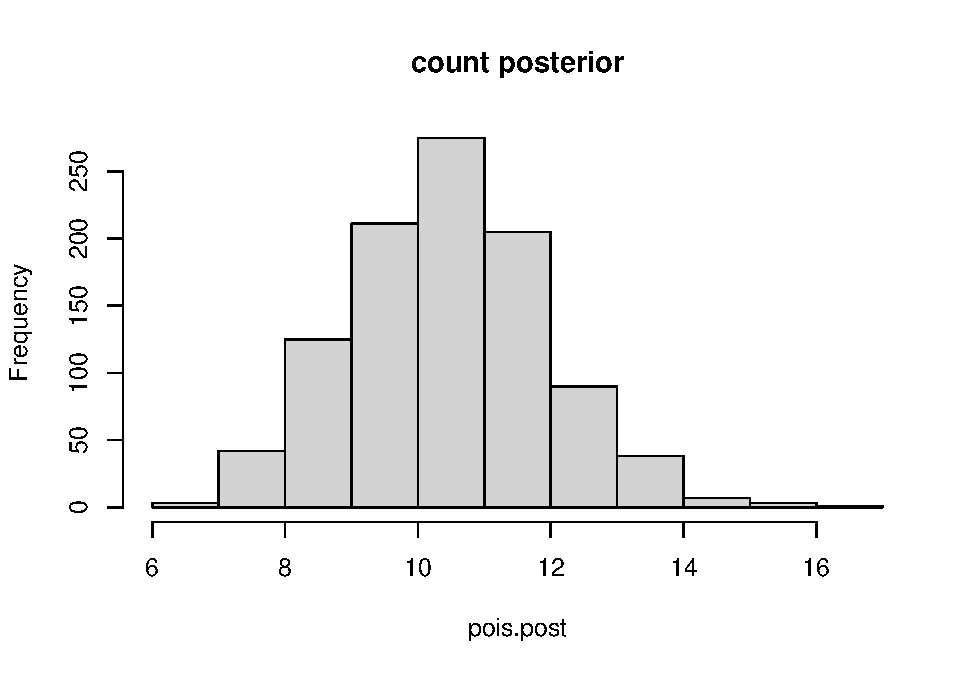
\includegraphics{_main_files/figure-latex/unnamed-chunk-39-1.pdf}

\begin{Shaded}
\begin{Highlighting}[]
  \CommentTok{\# post summary  mean : 8.8,  var= 1.47}
  \FunctionTok{summary}\NormalTok{(pois.post)}
\end{Highlighting}
\end{Shaded}

\begin{verbatim}
##    Min. 1st Qu.  Median    Mean 3rd Qu.    Max. 
##   6.966   9.369  10.288  10.370  11.289  15.032
\end{verbatim}

\begin{Shaded}
\begin{Highlighting}[]
  \FunctionTok{mean}\NormalTok{(pois.post)}
\end{Highlighting}
\end{Shaded}

\begin{verbatim}
## [1] 10.37015
\end{verbatim}

\begin{Shaded}
\begin{Highlighting}[]
  \FunctionTok{var}\NormalTok{(pois.post)}
\end{Highlighting}
\end{Shaded}

\begin{verbatim}
## [1] 1.976001
\end{verbatim}

\begin{Shaded}
\begin{Highlighting}[]
  \FunctionTok{plot}\NormalTok{(}\FunctionTok{density}\NormalTok{(pois.post),}\AttributeTok{ylim=}\FunctionTok{c}\NormalTok{(}\DecValTok{0}\NormalTok{,}\FloatTok{0.4}\NormalTok{),}\AttributeTok{main=}\StringTok{\textquotesingle{}pois posterior\textquotesingle{}}\NormalTok{)}
  \FunctionTok{lines}\NormalTok{(}\FunctionTok{density}\NormalTok{(obs),}\AttributeTok{col=}\StringTok{\textquotesingle{}red\textquotesingle{}}\NormalTok{)}
\end{Highlighting}
\end{Shaded}

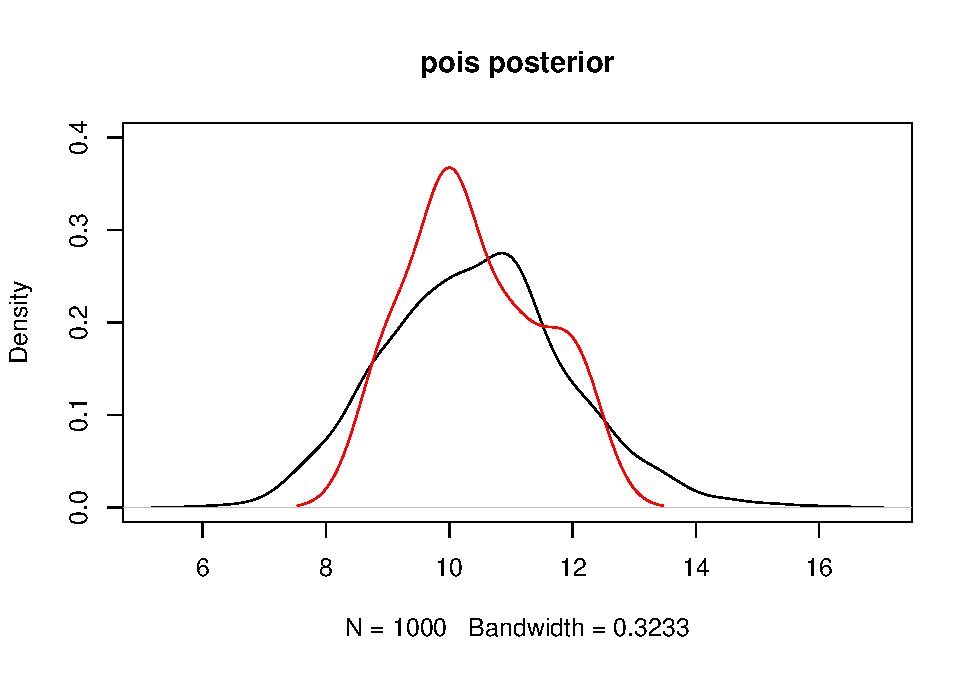
\includegraphics{_main_files/figure-latex/unnamed-chunk-39-2.pdf}

\begin{itemize}
\item
  \begin{enumerate}
  \def\labelenumi{(\alph{enumi})}
  \setcounter{enumi}{1}
  \tightlist
  \item
    Give the correct posterior distribution treating the measurements as rounded
    Using non informative prior for both unknowns, the posterior mean is 10.4 and posterior variance is 0.433
  \end{enumerate}
\end{itemize}

\begin{Shaded}
\begin{Highlighting}[]
 \DocumentationTok{\#\# normal with 2 unknowns.}
 \DocumentationTok{\#\# joint poisterior}
 \DocumentationTok{\#\# need the  sigma2 | y \textasciitilde{} inv{-}x2(n{-}1,s2)}
\NormalTok{  nu }\OtherTok{=} \FunctionTok{length}\NormalTok{(obs)}\SpecialCharTok{{-}}\DecValTok{1}
\NormalTok{  s2 }\OtherTok{=} \FunctionTok{var}\NormalTok{(obs)}
\NormalTok{  chi2}\OtherTok{=} \FunctionTok{rchisq}\NormalTok{(}\DecValTok{1000}\NormalTok{, nu)}
   \DocumentationTok{\#\# inv{-}chi2  v*s\^{}2/X  (Appendix A)}
\NormalTok{  sigma2 }\OtherTok{=}\NormalTok{ nu}\SpecialCharTok{*}\NormalTok{s2}\SpecialCharTok{/}\NormalTok{chi2}
  \DocumentationTok{\#\# posterior prob   =  p(m | sigma2, y)p(sigma2|y)}
   \DocumentationTok{\#\# for each variance term  draw   N( ybar,  sd= sqrt(sigma2/n))}
\NormalTok{  y}\OtherTok{\textless{}{-}}\FunctionTok{sapply}\NormalTok{(sigma2,}\ControlFlowTok{function}\NormalTok{(x) }\FunctionTok{rnorm}\NormalTok{(}\DecValTok{1}\NormalTok{, }\AttributeTok{mean=}\FunctionTok{mean}\NormalTok{(obs), }\AttributeTok{sd=}\FunctionTok{sqrt}\NormalTok{(x)}\SpecialCharTok{/}\FunctionTok{sqrt}\NormalTok{(}\DecValTok{5}\NormalTok{)))}
  \FunctionTok{hist}\NormalTok{(y,}\AttributeTok{main=}\StringTok{\textquotesingle{}posterior normal\textquotesingle{}}\NormalTok{)}
\end{Highlighting}
\end{Shaded}

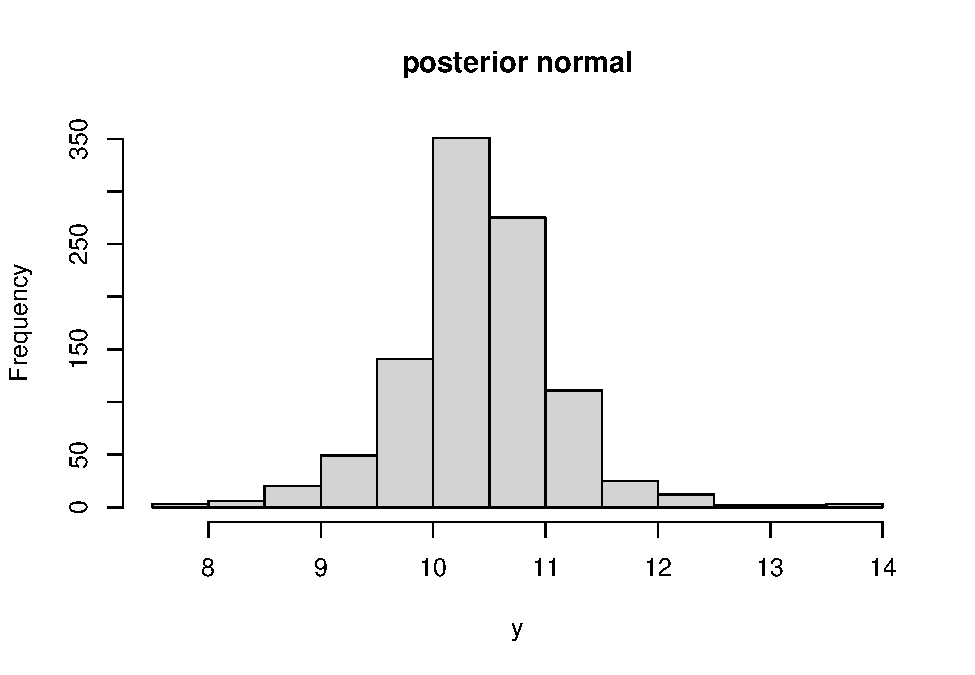
\includegraphics{_main_files/figure-latex/unnamed-chunk-40-1.pdf}

\begin{Shaded}
\begin{Highlighting}[]
  \FunctionTok{plot}\NormalTok{(}\FunctionTok{density}\NormalTok{(y),}\AttributeTok{main=}\StringTok{\textquotesingle{}posterior normal density\textquotesingle{}}\NormalTok{)}
  \FunctionTok{lines}\NormalTok{(}\FunctionTok{density}\NormalTok{(obs),}\AttributeTok{col=}\StringTok{\textquotesingle{}red\textquotesingle{}}\NormalTok{)}
\end{Highlighting}
\end{Shaded}

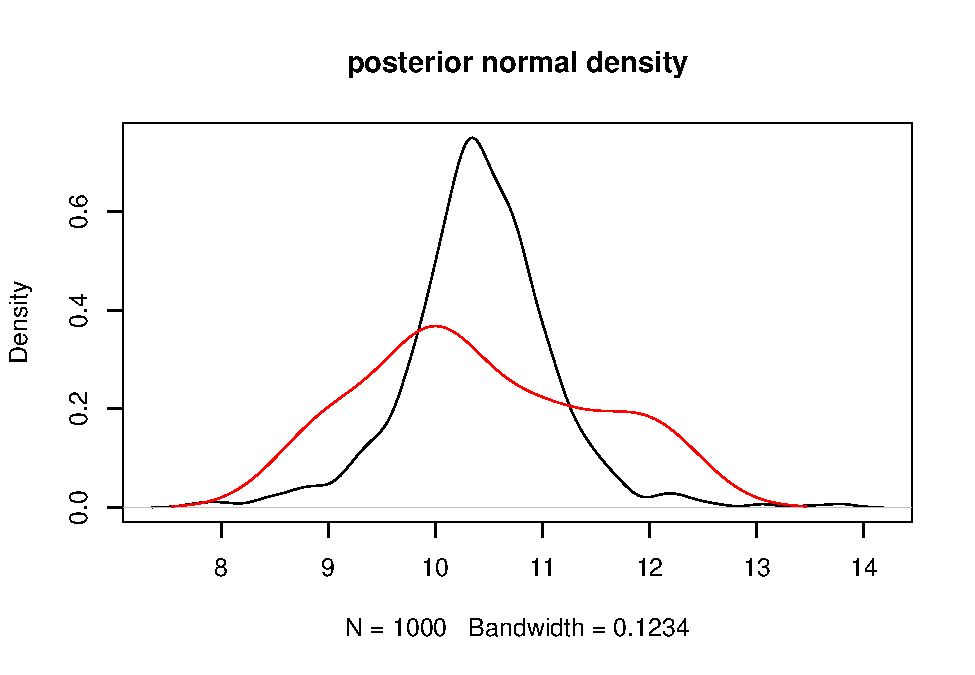
\includegraphics{_main_files/figure-latex/unnamed-chunk-40-2.pdf}
- (c) how do the correct/incorrect differ, compare means/variances

The difference in means is approximately 0, with a variance (residual) of 2.7.

\begin{Shaded}
\begin{Highlighting}[]
 \FunctionTok{mean}\NormalTok{( y }\SpecialCharTok{{-}}\NormalTok{ pois.post) }\CommentTok{\# 0.002926538}
\end{Highlighting}
\end{Shaded}

\begin{verbatim}
## [1] 0.03183058
\end{verbatim}

\begin{Shaded}
\begin{Highlighting}[]
 \FunctionTok{var}\NormalTok{( y }\SpecialCharTok{{-}}\NormalTok{ pois.post) }\CommentTok{\# 2.7}
\end{Highlighting}
\end{Shaded}

\begin{verbatim}
## [1] 2.513469
\end{verbatim}

\begin{Shaded}
\begin{Highlighting}[]
 \FunctionTok{hist}\NormalTok{(y}\SpecialCharTok{{-}}\NormalTok{pois.post)}
\end{Highlighting}
\end{Shaded}

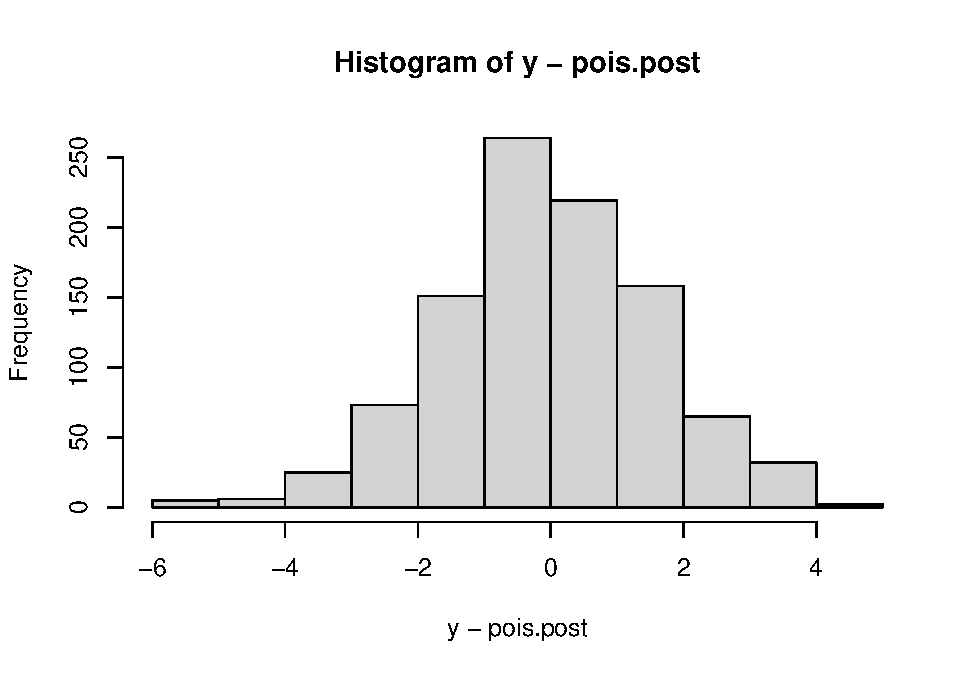
\includegraphics{_main_files/figure-latex/unnamed-chunk-41-1.pdf}

\begin{Shaded}
\begin{Highlighting}[]
 \FunctionTok{plot}\NormalTok{(y,pois.post,}\AttributeTok{main=}\StringTok{"normal vs. pois likelihoods"}\NormalTok{)}
\end{Highlighting}
\end{Shaded}

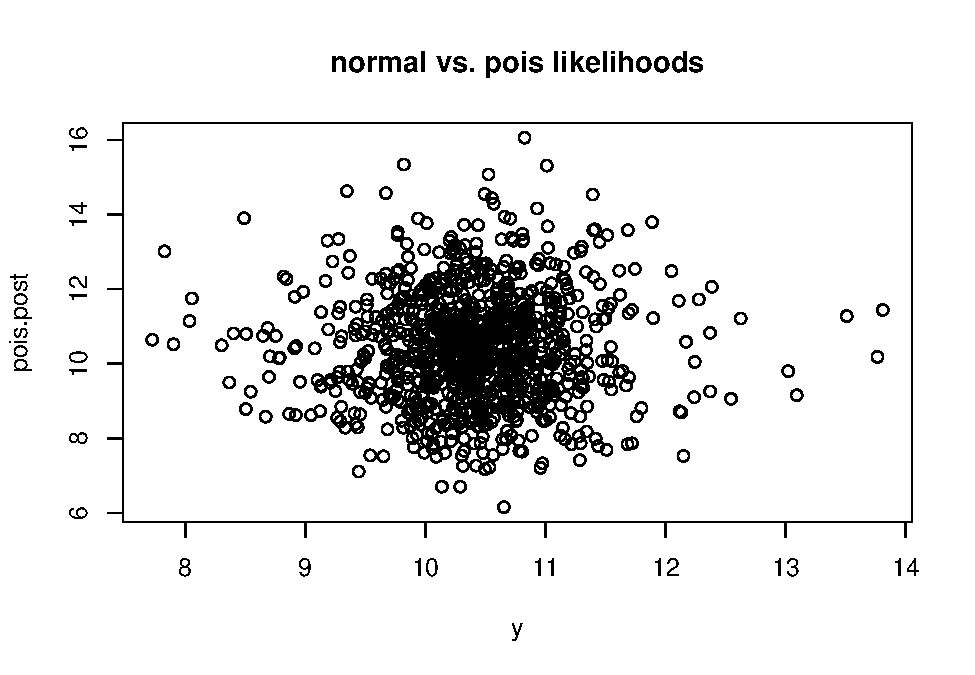
\includegraphics{_main_files/figure-latex/unnamed-chunk-41-2.pdf}

\begin{itemize}
\item
  \begin{enumerate}
  \def\labelenumi{(\alph{enumi})}
  \setcounter{enumi}{3}
  \tightlist
  \item
    Let z=(z1,z2,z3,z4,z5) be the original unrounded measurements corresponding to the five observations above. draw simulations of z and compare the posterior \((z1-z2)^2\).
  \end{enumerate}
\end{itemize}

For this we sample from the normal posterior distribution, conditioned on the rounded values to match the observed. For each sample of the posterior, the rounded values are conditioned to match the observed data. The mean difference of (\(z_1-z_2)^2\) is 0.14, with variance of 0.03.

\begin{Shaded}
\begin{Highlighting}[]
\NormalTok{ generateObs}\OtherTok{\textless{}{-}}\ControlFlowTok{function}\NormalTok{(obs)\{}
\NormalTok{   z}\OtherTok{\textless{}{-}}\ConstantTok{NULL}
    \ControlFlowTok{for}\NormalTok{(i }\ControlFlowTok{in} \DecValTok{1}\SpecialCharTok{:}\DecValTok{5}\NormalTok{)\{}
\NormalTok{ zi}\OtherTok{=} \FunctionTok{sample}\NormalTok{(y,}\DecValTok{1}\NormalTok{)}
  \ControlFlowTok{while}\NormalTok{( }\FunctionTok{round}\NormalTok{(zi)}\SpecialCharTok{!=}\NormalTok{obs[i])\{}
\NormalTok{    zi}\OtherTok{=}\FunctionTok{sample}\NormalTok{(y,}\DecValTok{1}\NormalTok{)}
\NormalTok{  \}}
\NormalTok{  z}\OtherTok{\textless{}{-}}\FunctionTok{c}\NormalTok{(z,zi)}
\NormalTok{    \}}
   \FunctionTok{stopifnot}\NormalTok{(}\FunctionTok{all}\NormalTok{(}\FunctionTok{round}\NormalTok{(z)}\SpecialCharTok{==}\NormalTok{obs))}
   \FunctionTok{return}\NormalTok{(z)}
\NormalTok{ \}}
 
\NormalTok{ ERR}\OtherTok{\textless{}{-}}\ConstantTok{NULL}

 \ControlFlowTok{for}\NormalTok{(j }\ControlFlowTok{in} \DecValTok{1}\SpecialCharTok{:}\DecValTok{1000}\NormalTok{)\{}
   \DocumentationTok{\#\# generate z samples such that round(z) == obs}
\NormalTok{  z}\OtherTok{\textless{}{-}}\FunctionTok{generateObs}\NormalTok{(obs)}
\NormalTok{  err}\OtherTok{\textless{}{-}}\NormalTok{ (z[}\DecValTok{1}\NormalTok{]}\SpecialCharTok{{-}}\NormalTok{z[}\DecValTok{2}\NormalTok{])}\SpecialCharTok{\^{}}\DecValTok{2}
\NormalTok{ ERR}\OtherTok{\textless{}{-}}\FunctionTok{c}\NormalTok{(ERR,err)}
\NormalTok{ \}}
 \FunctionTok{message}\NormalTok{(}\StringTok{"mean error:"}\NormalTok{,}\FunctionTok{mean}\NormalTok{(ERR))}
\end{Highlighting}
\end{Shaded}

\begin{verbatim}
## mean error:0.124189268711817
\end{verbatim}

\begin{Shaded}
\begin{Highlighting}[]
 \FunctionTok{hist}\NormalTok{(ERR)}
\end{Highlighting}
\end{Shaded}

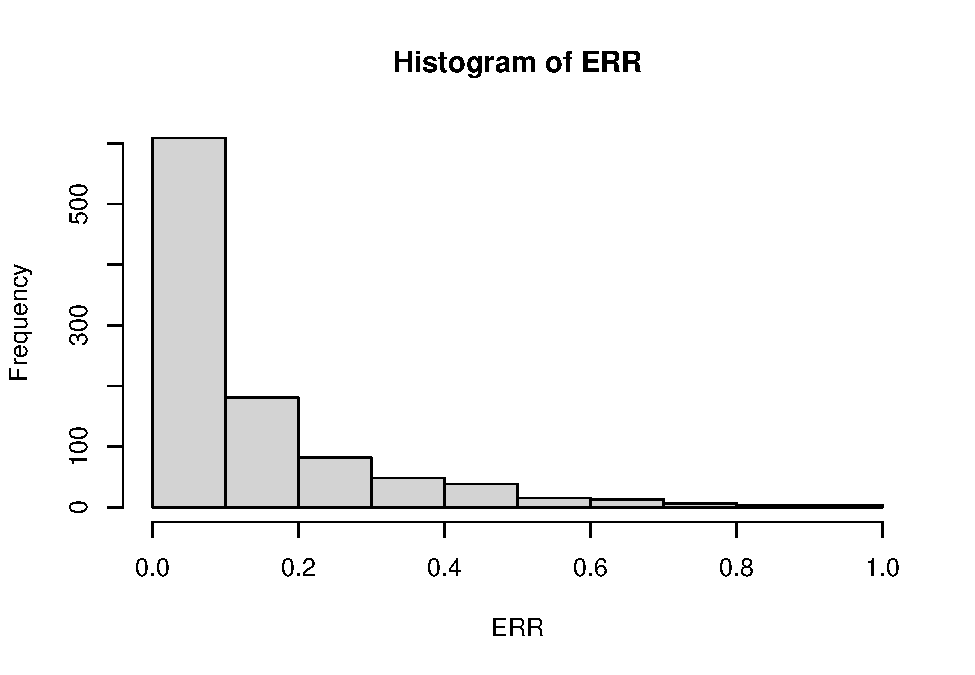
\includegraphics{_main_files/figure-latex/unnamed-chunk-42-1.pdf}
\#\# Question 6\{-\}
Consider data y1,\ldots,yn modeled as independent Bin(N,\(\theta\)) with both N and \(\theta\) unknown.

First we examine that \(p(\lambda,\theta)\propto 1/\lambda\) described by Raftery (1988). We take the product of a vague prior for \(\lambda\) and the uniform prior for \(\theta\). let \(\theta \sim U[0,1]\) be uniform and use the uniform prior for \(\lambda\) as a vague prior. The motivation here is to use a uniform vague prior on the hyperparameter. Alternatively we can use Jeffreys' Prior for Pois(\(\lambda) = 1/\sqrt{\lambda}\) where the \(-E(\partial l^2 / \partial \lambda^2) = 1/\lambda\) is known for the Poisson.
\[
\begin{aligned}
 p(\lambda,\theta) &\propto (1)1/\lambda\\
 &\propto \lambda^{-1}\\
\end{aligned}
\]
- (a) to write the prior N\(\sim P(\lambda)\) as a sampling distribution, but we can let N follow a Gamma, with a Gamma(0,0) vague prior initially and independent of \(\theta\). where \(\theta \sim U(0,1)\) as a uniform probability. Then \(P(N,\theta) = P(N|\theta)p(\theta)\). Note this is an improprer prior.\\
\[
\begin{aligned}
 p(N,\theta) &\propto (1)e^{-\beta*N}N^{\alpha-1}\\
 &\propto N^{-1}, \text{for  } \alpha,\beta =0\\
\end{aligned}
\]
We can solve for \(p(N,\theta)\) using the prior \(p(\lambda,\theta)\propto \lambda^{-1}\). and \(N\sim Pois(\lambda)\).
\[ 
\begin{aligned}
p(N,\lambda,\theta) &= p(N|\lambda,\theta)p(\lambda,\theta) \to p(N,\theta) = \int p(N,\lambda,\theta)d\lambda \\
&= \int \frac{(\lambda/N)^Ne^{-\lambda/\theta}}{N!}(\frac{1}{\lambda}) d\lambda\\
&= \frac{1}{N! \theta^N} \int \lambda^{N-1}e^{-\lambda/\theta}d\lambda\\
&= \frac{1}{N! \theta^N}\frac{\Gamma{(N)}}{1/\theta^N} = 1/N\\
\end{aligned}
\]
So we can let N follow vague prior from the Gamma(0,0) distribution, or call N a uniform on (0,N) and independent of \(\lambda\) to derive p(N,\(\theta)\).

\begin{itemize}
\item
  \begin{enumerate}
  \def\labelenumi{(\alph{enumi})}
  \setcounter{enumi}{1}
  \tightlist
  \item
    we need to find the marginal posterior of N, first we find the joint posterior which follows a Beta distribution
  \end{enumerate}
\end{itemize}

\[
\begin{aligned}
p(\theta,N | y) &=  p(y | N,\theta)p(N,\theta) \\
&\propto \theta^{\sum y_i} (1-\theta)^{nN-\sum y_i}(1/N)\\
&\propto (1/N)Beta(\sum y_i+1, nN-\sum y_i +1)\\
\end{aligned}
\]
Then we integrate with respect to \(\theta\) to find the marginal posterior, where the integrand is the kernel for the Beta distribution, and we have the beta coefficient that remains in the marginal equation.

\[
\begin{aligned}
 p(N| y) &= \int (1/N) \prod {N \choose y_i} \theta^{S}(1-\theta)^{nN-S}d\theta, S=\sum y_i \\
 & = (1/N) \prod {N \choose y_i} \int \theta^{S}(1-\theta)^{nN-S}d\theta \\
 & = (1/N) \prod {N \choose y_i} Beta(S+1, nN-S+1)\\
\end{aligned}
\]
The maximum probability is 122 trials with the highest marginal,

\begin{Shaded}
\begin{Highlighting}[]
\NormalTok{ x}\OtherTok{\textless{}{-}}\FunctionTok{c}\NormalTok{(}\DecValTok{53}\NormalTok{,}\DecValTok{57}\NormalTok{,}\DecValTok{66}\NormalTok{,}\DecValTok{67}\NormalTok{,}\DecValTok{72}\NormalTok{)}
\NormalTok{ totalN}\OtherTok{=}\FunctionTok{seq}\NormalTok{(}\FunctionTok{max}\NormalTok{(x),}\DecValTok{1000}\NormalTok{)}
 
\NormalTok{ marginal.post}\OtherTok{\textless{}{-}}\ControlFlowTok{function}\NormalTok{(N,x)\{}
\NormalTok{   n}\OtherTok{=}\FunctionTok{length}\NormalTok{(x)}
\NormalTok{   S}\OtherTok{=}\FunctionTok{sum}\NormalTok{(x)}
   \CommentTok{\# choose on the log scale}
\NormalTok{   a}\OtherTok{\textless{}{-}}\FunctionTok{sum}\NormalTok{( }\FunctionTok{lchoose}\NormalTok{(N,x))}
\NormalTok{    b }\OtherTok{=}\NormalTok{ (}\SpecialCharTok{{-}}\DecValTok{1}\NormalTok{)}\SpecialCharTok{*}\FunctionTok{log}\NormalTok{(N)}
  \CommentTok{\# b=0}
\NormalTok{   c }\OtherTok{=} \FunctionTok{lbeta}\NormalTok{( S}\SpecialCharTok{+}\DecValTok{1}\NormalTok{, n}\SpecialCharTok{*}\NormalTok{N}\SpecialCharTok{{-}}\NormalTok{ S }\SpecialCharTok{+}\DecValTok{1}\NormalTok{)}
   
   \CommentTok{\#rez\textless{}{-}(a*b)/c}
\NormalTok{   rez}\OtherTok{\textless{}{-}}\NormalTok{a}\SpecialCharTok{+}\NormalTok{b}\SpecialCharTok{+}\NormalTok{c}
   \FunctionTok{return}\NormalTok{(}\FunctionTok{exp}\NormalTok{(rez))}
\NormalTok{ \} }\DocumentationTok{\#\# problems here}
 
 \DocumentationTok{\#\# can we condition we can derive the analytic form of the joint posterior.}
 \DocumentationTok{\#\# }
\NormalTok{  marg.n}\OtherTok{\textless{}{-}}\FunctionTok{sapply}\NormalTok{(totalN,}\ControlFlowTok{function}\NormalTok{(y) }\FunctionTok{marginal.post}\NormalTok{(y,x))}
 \DocumentationTok{\#\# we use a grid approach to theta}
\NormalTok{totalN[}\FunctionTok{which.max}\NormalTok{(}\FunctionTok{exp}\NormalTok{(marg.n))]}
\end{Highlighting}
\end{Shaded}

\begin{verbatim}
## [1] 122
\end{verbatim}

\begin{Shaded}
\begin{Highlighting}[]
  \DocumentationTok{\#\#}
\NormalTok{norm.n}\OtherTok{\textless{}{-}}\NormalTok{marg.n}\SpecialCharTok{/}\FunctionTok{sum}\NormalTok{(marg.n)}
\FunctionTok{plot}\NormalTok{(totalN,norm.n)}
\FunctionTok{abline}\NormalTok{(}\AttributeTok{v=}\NormalTok{totalN[}\FunctionTok{which.max}\NormalTok{(}\FunctionTok{exp}\NormalTok{(marg.n))])}
\end{Highlighting}
\end{Shaded}

\includegraphics{_main_files/figure-latex/unnamed-chunk-43-1.pdf}
The joint posterior distribution given the data and N=122 (which was maximal marginal) has the maximum theta = 0.52.

\begin{Shaded}
\begin{Highlighting}[]
\NormalTok{ theta}\OtherTok{=}\FunctionTok{seq}\NormalTok{(}\FloatTok{0.01}\NormalTok{,}\FloatTok{0.99}\NormalTok{,}\AttributeTok{by=}\FloatTok{0.01}\NormalTok{)}

\NormalTok{ posterior.joint}\OtherTok{\textless{}{-}}\FunctionTok{dbeta}\NormalTok{(theta, }\FunctionTok{sum}\NormalTok{(x)}\SpecialCharTok{+}\DecValTok{1}\NormalTok{, }\DecValTok{5}\SpecialCharTok{*}\DecValTok{122}\SpecialCharTok{{-}}\FunctionTok{sum}\NormalTok{(x)}\SpecialCharTok{+}\DecValTok{1}\NormalTok{)}\SpecialCharTok{/}\DecValTok{122}
\NormalTok{ norm.post}\OtherTok{\textless{}{-}}\NormalTok{posterior.joint}\SpecialCharTok{/}\FunctionTok{sum}\NormalTok{(posterior.joint)}
  \FunctionTok{plot}\NormalTok{(theta,norm.post, }\AttributeTok{main=}\StringTok{\textquotesingle{}joint posterior N=122\textquotesingle{}}\NormalTok{)}
\end{Highlighting}
\end{Shaded}

\includegraphics{_main_files/figure-latex/unnamed-chunk-44-1.pdf}

\begin{Shaded}
\begin{Highlighting}[]
\NormalTok{  theta[}\FunctionTok{which.max}\NormalTok{(norm.post)]}
\end{Highlighting}
\end{Shaded}

\begin{verbatim}
## [1] 0.52
\end{verbatim}

\begin{itemize}
\tightlist
\item
  (b ii) and for P\((N>100) \approx 0.95\). We had to use the normalized marginal posterior distribution to correctly compute the probability.
\end{itemize}

\begin{Shaded}
\begin{Highlighting}[]
\DecValTok{1}\SpecialCharTok{{-}}\FunctionTok{sum}\NormalTok{(norm.n[totalN}\SpecialCharTok{\textless{}=}\DecValTok{100}\NormalTok{])}
\end{Highlighting}
\end{Shaded}

\begin{verbatim}
## [1] 0.9518952
\end{verbatim}

\begin{itemize}
\item
  \begin{enumerate}
  \def\labelenumi{(\alph{enumi})}
  \setcounter{enumi}{3}
  \tightlist
  \item
    the poisson distribution using \(\mu\) for N only gives the probability for N as a fixed realization, however we want to study the uncertainity over all possible N values.
  \end{enumerate}
\end{itemize}

\hypertarget{question-7-1}{%
\section*{Question 7}\label{question-7-1}}
\addcontentsline{toc}{section}{Question 7}

for 2 independent poisson distributions for x and y with \(\lambda_1,\lambda_2\). And the outcome \(X\) has a binomial distribution with N=x+y and unknown p.~show that the two models have the same likelihood.

We need to solve for the conditional probability of X given X+Y using the Poisson likelihoods. Here if you input the Poisson likelihoods, and use X+Y \(\sim Poi(\lambda_1+\lambda_2)\) this returns to a Binomial(n, \(\lambda_1/(\lambda_1+\lambda_2))\).
\[
\begin{aligned}
p(X =k| X+Y=n) &= \frac{P(X+Y=n | X=k)P(X=k)}{P(X+Y=n)} \\
 &=  \frac{P(Y=n-k)P(X=k)}{P(X+Y=n)} \\
\end{aligned}
\]

\hypertarget{question-8}{%
\section*{question 8}\label{question-8}}
\addcontentsline{toc}{section}{question 8}

notes: dirichlet distribution?
- (a) For a given block there are only two outcomes, bicycles, and other vehicles. So a binomial distribution is appropriate (2 outcomes only). We model y and binomial \((N_y,\theta_y)\) independent of z\(\sim Binomial(N_z,\theta_z)\).

We assume \(\theta_y,\theta_z\) are independent, so the posteriors are independent Beta models.
\[
\begin{aligned}
p(\theta_y,\theta_z| y,z) &= p(\theta_y | y)p(\theta_z|z) \\
&= Beta(\theta_y  | 1/2 +\sum y_i, 1/2+N_y-\sum y_i)*Beta(\theta_z  | 1/2 +\sum z_i, 1/2+N_z-\sum z_i)\\
\end{aligned}
\]
- (b) the prior uses Jeffreys' Beta(1/2,1/2) for each parameter independently.

\begin{Shaded}
\begin{Highlighting}[]
\NormalTok{rez.lane.bike}\OtherTok{\textless{}{-}}\FunctionTok{c}\NormalTok{(}\DecValTok{16}\NormalTok{,}\DecValTok{9}\NormalTok{,}\DecValTok{10}\NormalTok{,}\DecValTok{13}\NormalTok{,}\DecValTok{19}\NormalTok{,}\DecValTok{20}\NormalTok{,}\DecValTok{18}\NormalTok{,}\DecValTok{17}\NormalTok{,}\DecValTok{35}\NormalTok{,}\DecValTok{55}\NormalTok{)}
\NormalTok{rez.lane.other}\OtherTok{\textless{}{-}}\FunctionTok{c}\NormalTok{(}\DecValTok{58}\NormalTok{,}\DecValTok{90}\NormalTok{,}\DecValTok{48}\NormalTok{,}\DecValTok{57}\NormalTok{,}\DecValTok{103}\NormalTok{,}\DecValTok{57}\NormalTok{,}\DecValTok{86}\NormalTok{,}\DecValTok{112}\NormalTok{,}\DecValTok{273}\NormalTok{,}\DecValTok{64}\NormalTok{)}
\NormalTok{NY}\OtherTok{\textless{}{-}}\NormalTok{(rez.lane.bike}\SpecialCharTok{+}\NormalTok{rez.lane.other)}
\NormalTok{rez.lane.p}\OtherTok{\textless{}{-}}\NormalTok{rez.lane.bike}\SpecialCharTok{/}\NormalTok{(rez.lane.bike}\SpecialCharTok{+}\NormalTok{rez.lane.other)}

\NormalTok{rez.nolane.bike}\OtherTok{\textless{}{-}}\FunctionTok{c}\NormalTok{(}\DecValTok{12}\NormalTok{,}\DecValTok{1}\NormalTok{,}\DecValTok{2}\NormalTok{,}\DecValTok{4}\NormalTok{,}\DecValTok{9}\NormalTok{,}\DecValTok{7}\NormalTok{,}\DecValTok{9}\NormalTok{,}\DecValTok{8}\NormalTok{)}
\NormalTok{rez.nolane.other}\OtherTok{\textless{}{-}}\FunctionTok{c}\NormalTok{(}\DecValTok{113}\NormalTok{,}\DecValTok{18}\NormalTok{,}\DecValTok{14}\NormalTok{,}\DecValTok{44}\NormalTok{,}\DecValTok{208}\NormalTok{,}\DecValTok{67}\NormalTok{,}\DecValTok{29}\NormalTok{,}\DecValTok{154}\NormalTok{)}
\NormalTok{NZ}\OtherTok{\textless{}{-}}\NormalTok{(rez.nolane.bike}\SpecialCharTok{+}\NormalTok{rez.nolane.other)}

\NormalTok{rez.nolane.p}\OtherTok{\textless{}{-}}\NormalTok{rez.nolane.bike}\SpecialCharTok{/}\NormalTok{(rez.nolane.bike}\SpecialCharTok{+}\NormalTok{rez.nolane.other)}
\end{Highlighting}
\end{Shaded}

\begin{itemize}
\item
  \begin{enumerate}
  \def\labelenumi{(\alph{enumi})}
  \setcounter{enumi}{2}
  \tightlist
  \item
    we determine the posterior distribution using the beta distribution by sampline independently. Using a grid a pproach we see the contour map centered around 0.18 and 0.09 which is equivalent to the MLEs.
  \end{enumerate}
\end{itemize}

\begin{Shaded}
\begin{Highlighting}[]
\NormalTok{bike.post}\OtherTok{\textless{}{-}}\FunctionTok{rbeta}\NormalTok{(}\DecValTok{1000}\NormalTok{, (}\DecValTok{1}\SpecialCharTok{/}\DecValTok{2} \SpecialCharTok{+} \FunctionTok{sum}\NormalTok{(rez.lane.bike)), (}\DecValTok{1}\SpecialCharTok{/}\DecValTok{2}\SpecialCharTok{+}\FunctionTok{sum}\NormalTok{(rez.lane.other)))}
\NormalTok{bike.post2}\OtherTok{\textless{}{-}}\FunctionTok{rbeta}\NormalTok{(}\DecValTok{1000}\NormalTok{, (}\DecValTok{1}\SpecialCharTok{/}\DecValTok{2} \SpecialCharTok{+} \FunctionTok{sum}\NormalTok{(rez.nolane.bike)), (}\DecValTok{1}\SpecialCharTok{/}\DecValTok{2}\SpecialCharTok{+}\FunctionTok{sum}\NormalTok{(rez.nolane.other)))}



\NormalTok{p0}\OtherTok{=} \FunctionTok{seq}\NormalTok{(}\FloatTok{0.01}\NormalTok{,}\FloatTok{0.99}\NormalTok{,}\AttributeTok{by=}\FloatTok{0.01}\NormalTok{)}
\NormalTok{p1}\OtherTok{=} \FunctionTok{seq}\NormalTok{(}\FloatTok{0.01}\NormalTok{,}\FloatTok{0.99}\NormalTok{,}\AttributeTok{by=}\FloatTok{0.01}\NormalTok{)}


\NormalTok{post.bike}\OtherTok{\textless{}{-}}\ControlFlowTok{function}\NormalTok{(p0,p1,y,z,ny,nz)\{}
\NormalTok{  pos}\OtherTok{\textless{}{-}}\NormalTok{ p0}\SpecialCharTok{\^{}}\NormalTok{(}\FunctionTok{sum}\NormalTok{(y))}\SpecialCharTok{*}\NormalTok{(}\DecValTok{1}\SpecialCharTok{{-}}\NormalTok{p0)}\SpecialCharTok{\^{}}\NormalTok{(}\FunctionTok{sum}\NormalTok{(ny)}\SpecialCharTok{{-}}\FunctionTok{sum}\NormalTok{(y))}\SpecialCharTok{*}\NormalTok{p1}\SpecialCharTok{\^{}}\NormalTok{(}\FunctionTok{sum}\NormalTok{(z))}\SpecialCharTok{*}\NormalTok{(}\DecValTok{1}\SpecialCharTok{{-}}\NormalTok{p1)}\SpecialCharTok{\^{}}\NormalTok{(}\FunctionTok{sum}\NormalTok{(nz)}\SpecialCharTok{{-}}\FunctionTok{sum}\NormalTok{(z))}\SpecialCharTok{*}\FunctionTok{dbeta}\NormalTok{(p0,}\DecValTok{1}\SpecialCharTok{/}\DecValTok{2}\NormalTok{,}\DecValTok{1}\SpecialCharTok{/}\DecValTok{2}\NormalTok{)}\SpecialCharTok{*}\FunctionTok{dbeta}\NormalTok{(p1,}\DecValTok{1}\SpecialCharTok{/}\DecValTok{2}\NormalTok{,}\DecValTok{1}\SpecialCharTok{/}\DecValTok{2}\NormalTok{)}
  \FunctionTok{return}\NormalTok{(pos)}
\NormalTok{\}}
\NormalTok{ posts}\OtherTok{\textless{}{-}}\ConstantTok{NULL}
 
\NormalTok{p0p1}\OtherTok{\textless{}{-}} \FunctionTok{expand.grid}\NormalTok{(p0, p1)}

\ControlFlowTok{for}\NormalTok{(i }\ControlFlowTok{in} \DecValTok{1}\SpecialCharTok{:}\FunctionTok{nrow}\NormalTok{(p0p1))\{}
\NormalTok{  posts[i]}\OtherTok{\textless{}{-}}\FunctionTok{post.bike}\NormalTok{(p0p1[i,}\StringTok{"Var1"}\NormalTok{],p0p1[i,}\StringTok{"Var2"}\NormalTok{], rez.lane.bike,rez.nolane.bike, NY,NZ) }
\NormalTok{\}}
 \FunctionTok{library}\NormalTok{(ggplot2)}
 \FunctionTok{ggplot}\NormalTok{(p0p1)}\SpecialCharTok{+}
 \FunctionTok{geom\_contour}\NormalTok{(}\AttributeTok{mapping =} \FunctionTok{aes}\NormalTok{(}\AttributeTok{x =}\NormalTok{ Var1, }\AttributeTok{y =}\NormalTok{ Var2, }\AttributeTok{z =}\NormalTok{ posts), }\AttributeTok{bins =} \DecValTok{20}\NormalTok{)}
\end{Highlighting}
\end{Shaded}

\includegraphics{_main_files/figure-latex/unnamed-chunk-47-1.pdf}

\begin{itemize}
\item
  \begin{enumerate}
  \def\labelenumi{(\alph{enumi})}
  \setcounter{enumi}{3}
  \tightlist
  \item
    expected difference and the posterior distribution
    we find the difference in the posterior distribution which is approximately 0.11 higher proportions in bike routes.
  \end{enumerate}
\end{itemize}

\begin{Shaded}
\begin{Highlighting}[]
 \FunctionTok{hist}\NormalTok{(bike.post}\SpecialCharTok{{-}}\NormalTok{bike.post2)}
 \FunctionTok{abline}\NormalTok{(}\AttributeTok{v=}\FunctionTok{mean}\NormalTok{(bike.post)}\SpecialCharTok{{-}}\FunctionTok{mean}\NormalTok{(bike.post2))}
\end{Highlighting}
\end{Shaded}

\includegraphics{_main_files/figure-latex/unnamed-chunk-48-1.pdf}

\begin{Shaded}
\begin{Highlighting}[]
\NormalTok{ meany }\OtherTok{=}\NormalTok{(}\DecValTok{1}\SpecialCharTok{/}\DecValTok{2} \SpecialCharTok{+} \FunctionTok{sum}\NormalTok{(rez.lane.bike))}\SpecialCharTok{/}\NormalTok{(}\DecValTok{1}\SpecialCharTok{/}\DecValTok{2} \SpecialCharTok{+} \FunctionTok{sum}\NormalTok{(rez.lane.bike)}\SpecialCharTok{+}\NormalTok{(}\DecValTok{1}\SpecialCharTok{/}\DecValTok{2}\SpecialCharTok{+}\FunctionTok{sum}\NormalTok{(rez.lane.other))) }\DocumentationTok{\#\# theoretical mean}
\NormalTok{  meanz }\OtherTok{=}\NormalTok{(}\DecValTok{1}\SpecialCharTok{/}\DecValTok{2} \SpecialCharTok{+} \FunctionTok{sum}\NormalTok{(rez.nolane.bike))}\SpecialCharTok{/}\NormalTok{(}\DecValTok{1}\SpecialCharTok{/}\DecValTok{2} \SpecialCharTok{+} \FunctionTok{sum}\NormalTok{(rez.nolane.bike)}\SpecialCharTok{+}\NormalTok{(}\DecValTok{1}\SpecialCharTok{/}\DecValTok{2}\SpecialCharTok{+}\FunctionTok{sum}\NormalTok{(rez.nolane.other))) }\DocumentationTok{\#\# theoretical mean}
\end{Highlighting}
\end{Shaded}

\hypertarget{question-9}{%
\section*{question 9}\label{question-9}}
\addcontentsline{toc}{section}{question 9}

We need to derive the posterior of \(p(\mu^2, \sigma^2 | y)\). \(p(\mu,\sigma^2 | y) = p(y|\mu,\sigma^2)*p(\mu , \sigma^2)\)

\[
\begin{aligned}
p(\mu, \sigma^2 |y)&=\sigma^{-1}(\sigma^2)^{-(\nu_0/2 +1)}exp(-1/2\sigma^2 (\nu_0\sigma_0^2 + k_0(\mu-\mu_0)^2)) \times (\sigma^2)^{-n/2}exp(-1/2\sigma^2 ((n-1)s^2 + n(\mu-\bar{y})^2))\\
&= \sigma^{-1}(\sigma^2)^{-((\nu_0+n)/2 +1)} exp(-1/2\sigma^2( \nu_0\sigma_0^2 +(n-1)s^2 +\mu^2(k_0+n) +\mu(-2\mu_0k_0 -2\bar{y}n) + \mu_0^2k_0 +n\bar{y}^2)\\
\end{aligned}
\]
Where we factor the inside using \(\mu_n = k_0\mu_0/(k_0+n) +n\bar{y}/(k_0+n)\)
\[
\begin{aligned}
&\to \mu^2(k_0+n) +\mu(-2\mu_0k_0 -2\bar{y}n) + \mu_0^2k_0 +n\bar{y}^2 \\
&= (k_0+n)(\mu^2 - 2\mu( \mu_0k_0/(k_0+n) +\bar{y}n/(k_0+n)) + \mu_0^2k_0/(k_0+n) + n\bar{y}^2/(k_0+n)) \\
&= (k_0+n)(\mu^2 - 2\mu( k_0\mu_0/(k_0+n) +n\bar{y}/(k_0+n)) + \frac{\mu_0^2k_0(k_0+n)}{(k_0+n)^2} + \frac{n\bar{y}^2(k_0+n)}{(k_0+n)^2} +\frac{2k_0\mu_0n\bar{y}}{(k_0+n)^2} -\frac{2k_0\mu_0n\bar{y}}{(k_0+n)^2})\\
&= (k_0+n)(\mu^2 - 2\mu( k_0\mu_0/(k_0+n) +n\bar{y}/(k_0+n)) + \frac{\mu_0^2k_0^2}{(k_0+n)^2} +\frac{\mu_0^2k_0*n}{(k_0+n)^2}+ \frac{n^2\bar{y}^2}{(k_0+n)^2} + \frac{n\bar{y}^2k_0}{(k_0+n)^2}+\frac{2k_0\mu_0n\bar{y}}{(k_0+n)^2} -\frac{2k_0\mu_0n\bar{y}}{(k_0+n)^2}) \\
&= (k_0+n)(\mu^2 + -2\mu\mu_n +\mu_n^2  +\frac{\mu_0^2k_0*n}{(k_0+n)^2}+ \frac{n\bar{y}^2k_0}{(k_0+n)^2} -\frac{2k_0\mu_0n\bar{y}}{(k_0+n)^2})\\
&= (k_0+n)( (\mu-\mu_n)^2 + (k_0*n)/(k_0+n)^2( \mu_0^2+\bar{y}^2 -2\mu_0\bar{y}) \\
&=  (k_0+n)( (\mu-\mu_n)^2 + (k_0*n)/(k_0+n)( \mu_0-\bar{y})^2\\
\end{aligned}
\]

putting the factorization into the posterior and derived the formula for each updated term.

here we see that \(\sigma^2_n ,\mu_n\) are sufficient statistics for \(\mu,\sigma^2\) by the factorization theorem because the posterior depends on parameters only through the summary statistics.

\[
\begin{aligned}
p(\mu, \sigma^2 |y)&=\sigma^{-1}(\sigma^2)^{-((\nu_0+n)/2 +1)} exp(-1/2\sigma^2+ ( \nu_0\sigma_0^2 +(n-1)s^2 +(k_0+n)( (\mu-\mu_n)^2 + (k_0*n)/(k_0+n)( \mu_0-\bar{y})^2)\\
&= \sigma^{-1}(\sigma^2)^{-((\nu_0+n)/2 +1)} exp(-1/2\sigma^2+ ( \nu_n\sigma_n^2 +(k_n)( (\mu-\mu_n)^2 )\\
& = \sigma^{-1}(\sigma^2)^{-((\nu_n)/2 +1)} exp(-1/2\sigma^2 ( \nu_n\sigma_n^2 +(k_n)( (\mu-\mu_n)^2 )\\
\end{aligned}
\]
\# Question 10\{-\}
To show the F-distribution we prove it directly, using a change of variables. Although there is a theorem (definition) that for \(X\sim N(a,b)\) and \(Y\sim N(c,d)\) then F= \(S_X^2/\sigma^2_X / (S_Y^2 / \sigma_Y^2)\) follows an F-distribution.

For \((n-1)S^2/\sigma^2 \sim X_{n-1}^2\) we let \(U \sim \chi_p^2, V\sim \chi_q^2\). We let \(Z = (U/p)/(V/q)\) and \(W=V/q\).

\[
J= 
\begin{bmatrix}
 \partial u/\partial z & \partial u/\partial w \\
 \partial v/\partial z & \partial v/\partial w  
\end{bmatrix} = 
\begin{bmatrix}
 q & 0 \\
  zp& pw  \\
\end{bmatrix} = qpw
\]

For V = wq, and U = zpw. Note that after combining terms we have the Gamma kernel with \(\alpha = p+q/2 -1\) and \(\beta= 1/2(pz+q)\) which is the F-distribution.\\
\[
\begin{aligned}
f(z,w)&= f(u)f(v)|J| \\
 &= \frac{1}{\Gamma(p/2)2^{p/2}}(pzw)^{p/2-1}e^{-pzw/2}/frac{1}{\Gamma(q/2)2^{q/2}}(wq)^{q/2-1}e^{-wq/2}|pwq| \\
 &=\frac{z^{p/2-1}}{\Gamma(p/2)2^{p+q/2}\Gamma(q/2)}(p)^{p/2}q^{q/2}w^{(p+q/2 -1)} e^{-w/2(pz+q/2)} \\
 & = \frac{z^{p/2-1}}{\Gamma(p/2)2^{p+q/2}\Gamma(q/2)}(p)^{p/2}q^{q/2}[\frac{\Gamma(p+q/2)}{(1/2(pz+q))^{p+q/2}}]\\
 &= \frac{z^{p/2-1}}{\Gamma(p/2)\Gamma(q/2)}(p)^{p/2}q^{q/2}[\frac{\Gamma(p+q/2)}{(q^{p+q/2(pz/q+1))^{p+q/2}}}]\\
 &=\frac{z^{p/2-1}\Gamma(p+q/2)}{\Gamma(p/2)\Gamma(q/2)}(p/q)^{p/2}\frac{1}{(pz/q+1)^{p+q/2}} \\
\end{aligned}
\]

We showed that for U, V as Chi-square variables, their ratio is the F-distribution, In order to show that the posterior distribution F= \(S_X^2/\sigma^2_X / (S_Y^2 / \sigma_Y^2)\) is F. The posterior \(Y \sim \sigma^2 | y \sim Inv-\chi^2(\nu, \sigma^2)\). where Y =\(\frac{(n-1)S^2}{\chi_{n-1}^2}\). So The inverse chi-square distribution can be re-arranged to follow a Chi-square. Then the variable Z in terms of Chi-square variables can be expressed using Inv-Chisquare variables.

\hypertarget{question-11-1}{%
\section*{Question 11}\label{question-11-1}}
\addcontentsline{toc}{section}{Question 11}

the model is defined as \(p(\alpha,\beta,y,n,x) \propto p(\alpha,\beta)\prod_{i=1}^{4}p(y_i | \alpha,\beta,n_i,x_i)\), where \((\alpha,\beta)\) follows a joint normal prior with \(\alpha \sim N(0, 2^2)\) and \(\beta \sim N(10,10^2)\) and corr(\(\alpha,\beta) = 0.5\).

\begin{itemize}
\item
  \begin{enumerate}
  \def\labelenumi{(\alph{enumi})}
  \tightlist
  \item
    we repeat the computations of this data
  \end{enumerate}
\item
  \begin{enumerate}
  \def\labelenumi{(\alph{enumi})}
  \setcounter{enumi}{1}
  \tightlist
  \item
    and overlay the contour with the posterior distribution
  \end{enumerate}
\end{itemize}

\begin{Shaded}
\begin{Highlighting}[]
 \FunctionTok{library}\NormalTok{(mvtnorm)}
 \FunctionTok{library}\NormalTok{(magrittr)}
 \FunctionTok{library}\NormalTok{(dplyr)}
 \FunctionTok{library}\NormalTok{(ggplot2)}
\NormalTok{ assay}\OtherTok{\textless{}{-}}\FunctionTok{data.frame}\NormalTok{(}\AttributeTok{x=}\FunctionTok{c}\NormalTok{(}\SpecialCharTok{{-}}\FloatTok{0.86}\NormalTok{,}\SpecialCharTok{{-}}\FloatTok{0.30}\NormalTok{,}\SpecialCharTok{{-}}\FloatTok{0.05}\NormalTok{,}\FloatTok{0.73}\NormalTok{), }\AttributeTok{n=}\FunctionTok{c}\NormalTok{(}\DecValTok{5}\NormalTok{,}\DecValTok{5}\NormalTok{,}\DecValTok{5}\NormalTok{,}\DecValTok{5}\NormalTok{), }\AttributeTok{y=}\FunctionTok{c}\NormalTok{(}\DecValTok{0}\NormalTok{,}\DecValTok{1}\NormalTok{,}\DecValTok{3}\NormalTok{,}\DecValTok{5}\NormalTok{))}

 \DocumentationTok{\#\# the point a,b by MLE is (0.8,7.7) so we grid around these solution.}
\NormalTok{ a0}\OtherTok{=} \FunctionTok{seq}\NormalTok{(}\SpecialCharTok{{-}}\DecValTok{5}\NormalTok{,}\DecValTok{10}\NormalTok{,}\AttributeTok{by=}\FloatTok{0.1}\NormalTok{)}
\NormalTok{ b1}\OtherTok{=} \FunctionTok{seq}\NormalTok{(}\SpecialCharTok{{-}}\DecValTok{10}\NormalTok{,}\DecValTok{40}\NormalTok{,}\AttributeTok{by=}\FloatTok{0.1}\NormalTok{)}
\NormalTok{  a0b1}\OtherTok{\textless{}{-}} \FunctionTok{expand.grid}\NormalTok{(a0, b1)}

\NormalTok{logit}\OtherTok{\textless{}{-}}\ControlFlowTok{function}\NormalTok{(theta)\{}
  \FunctionTok{return}\NormalTok{( }\FunctionTok{log}\NormalTok{(theta}\SpecialCharTok{/}\NormalTok{(}\DecValTok{1}\SpecialCharTok{{-}}\NormalTok{theta)))}
\NormalTok{\}}

\NormalTok{inv.logit}\OtherTok{\textless{}{-}}\ControlFlowTok{function}\NormalTok{(theta)\{}
  \FunctionTok{return}\NormalTok{( (}\FunctionTok{exp}\NormalTok{(theta)}\SpecialCharTok{/}\NormalTok{(}\DecValTok{1}\SpecialCharTok{+}\FunctionTok{exp}\NormalTok{(theta)))  )}
\NormalTok{\}}

\DocumentationTok{\#\# alpha, beta come from multivariate normal.}
 \DocumentationTok{\#\# \textbackslash{}prod\_(i=1)\^{}5 p(y|theta) \textasciitilde{} \textbackslash{}theta\^{}y (1{-}theta)\^{}n{-}y \#\# kth dose. }
  \DocumentationTok{\#\#\# logit(theta) = alpha+ beta*x}
\NormalTok{logit.likelihood}\OtherTok{\textless{}{-}}\ControlFlowTok{function}\NormalTok{(alpha,beta,x,y,n)\{}
\NormalTok{   theta\_approx}\OtherTok{\textless{}{-}}\NormalTok{ alpha}\SpecialCharTok{+}\NormalTok{beta}\SpecialCharTok{*}\NormalTok{x}
\NormalTok{   bin.like}\OtherTok{\textless{}{-}}\NormalTok{(}\FunctionTok{inv.logit}\NormalTok{(theta\_approx))}\SpecialCharTok{\^{}}\NormalTok{y}\SpecialCharTok{*}\NormalTok{(}\DecValTok{1}\SpecialCharTok{{-}}\FunctionTok{inv.logit}\NormalTok{(theta\_approx))}\SpecialCharTok{\^{}}\NormalTok{(n}\SpecialCharTok{{-}}\NormalTok{y)}
   \FunctionTok{return}\NormalTok{(bin.like)}
\NormalTok{\}  }

 \DocumentationTok{\#\# the alpha,beta stem from the grid, and we return the probability mass from the prior.}
\NormalTok{ joint.prior}\OtherTok{\textless{}{-}}\ControlFlowTok{function}\NormalTok{(alpha,beta)\{}
\NormalTok{  cormat}\OtherTok{\textless{}{-}}\FunctionTok{matrix}\NormalTok{(}\FunctionTok{c}\NormalTok{(}\DecValTok{4}\NormalTok{,}\FloatTok{0.5}\SpecialCharTok{*}\DecValTok{2}\SpecialCharTok{*}\DecValTok{10}\NormalTok{,}\FloatTok{0.5}\SpecialCharTok{*}\DecValTok{2}\SpecialCharTok{*}\DecValTok{10}\NormalTok{,}\DecValTok{100}\NormalTok{),}\DecValTok{2}\NormalTok{)}
  \FunctionTok{return}\NormalTok{(}\FunctionTok{dmvnorm}\NormalTok{(}\FunctionTok{c}\NormalTok{(alpha,beta), }\AttributeTok{mean=}\FunctionTok{c}\NormalTok{(}\DecValTok{0}\NormalTok{,}\DecValTok{10}\NormalTok{),}\AttributeTok{sigma=}\NormalTok{cormat))}
\NormalTok{ \}}
  
\NormalTok{ posterior\_density}\OtherTok{\textless{}{-}}\ControlFlowTok{function}\NormalTok{(alpha,beta,assay)\{}
\NormalTok{   joint\_density}\OtherTok{\textless{}{-}}\FunctionTok{joint.prior}\NormalTok{(alpha,beta)}
\NormalTok{   probs}\OtherTok{\textless{}{-}}\ConstantTok{NULL}
   \ControlFlowTok{for}\NormalTok{(k }\ControlFlowTok{in} \DecValTok{1}\SpecialCharTok{:}\FunctionTok{nrow}\NormalTok{(assay))\{}
\NormalTok{     p}\OtherTok{\textless{}{-}}\FunctionTok{logit.likelihood}\NormalTok{(alpha,beta,assay}\SpecialCharTok{$}\NormalTok{x[k],assay}\SpecialCharTok{$}\NormalTok{y[k],assay}\SpecialCharTok{$}\NormalTok{n[k])}
\NormalTok{     probs}\OtherTok{\textless{}{-}}\FunctionTok{c}\NormalTok{(probs,p)}
\NormalTok{   \}}
\NormalTok{   totalLikelihood}\OtherTok{\textless{}{-}}\FunctionTok{prod}\NormalTok{(probs)}
   \FunctionTok{return}\NormalTok{( joint\_density}\SpecialCharTok{*}\NormalTok{totalLikelihood)}
\NormalTok{ \}}
 

\NormalTok{ posts}\OtherTok{\textless{}{-}}\ConstantTok{NULL}
 
 \DocumentationTok{\#\# unnormalized posterior over grid which covers (a,b)}
\ControlFlowTok{for}\NormalTok{(i }\ControlFlowTok{in} \DecValTok{1}\SpecialCharTok{:}\FunctionTok{nrow}\NormalTok{(a0b1))\{}
\NormalTok{  posts[i]}\OtherTok{\textless{}{-}}\FunctionTok{posterior\_density}\NormalTok{(a0b1[i,}\StringTok{"Var1"}\NormalTok{],a0b1[i,}\StringTok{"Var2"}\NormalTok{],assay) }
\NormalTok{\}}
 
\NormalTok{ posts\_norm}\OtherTok{\textless{}{-}}\NormalTok{posts}\SpecialCharTok{/}\FunctionTok{sum}\NormalTok{(posts)}
\NormalTok{ a0b1}\SpecialCharTok{$}\NormalTok{joint.prob}\OtherTok{\textless{}{-}}\NormalTok{posts\_norm}
 
 \DocumentationTok{\#\# grid sampling procedure}
\NormalTok{  marginal.post\_a}\OtherTok{\textless{}{-}}\NormalTok{ a0b1}\SpecialCharTok{\%\textgreater{}\%}\FunctionTok{group\_by}\NormalTok{(Var1)}\SpecialCharTok{\%\textgreater{}\%}\FunctionTok{summarise}\NormalTok{(}\AttributeTok{p=}\FunctionTok{sum}\NormalTok{(joint.prob))}\SpecialCharTok{\%\textgreater{}\%}\NormalTok{data.frame}
\NormalTok{    A}\OtherTok{\textless{}{-}}\NormalTok{B}\OtherTok{\textless{}{-}}\ConstantTok{NULL}
  \ControlFlowTok{for}\NormalTok{(s }\ControlFlowTok{in} \DecValTok{1}\SpecialCharTok{:}\DecValTok{1000}\NormalTok{)\{}
\NormalTok{    a\_s}\OtherTok{\textless{}{-}}\FunctionTok{sample}\NormalTok{(marginal.post\_a}\SpecialCharTok{$}\NormalTok{Var1,}\DecValTok{1}\NormalTok{,}\AttributeTok{prob=}\NormalTok{marginal.post\_a}\SpecialCharTok{$}\NormalTok{p)}
\NormalTok{    p.a\_s}\OtherTok{\textless{}{-}}\NormalTok{marginal.post\_a[}\FunctionTok{which}\NormalTok{(marginal.post\_a}\SpecialCharTok{$}\NormalTok{Var1}\SpecialCharTok{==}\NormalTok{a\_s),}\StringTok{\textquotesingle{}p\textquotesingle{}}\NormalTok{]}
\NormalTok{    marginal.post\_b}\OtherTok{\textless{}{-}}\NormalTok{a0b1[}\FunctionTok{which}\NormalTok{(a0b1}\SpecialCharTok{$}\NormalTok{Var1}\SpecialCharTok{==}\NormalTok{a\_s),]}
\NormalTok{    marginal.post\_b}\SpecialCharTok{$}\NormalTok{cond.prob}\OtherTok{\textless{}{-}}\NormalTok{marginal.post\_b}\SpecialCharTok{$}\NormalTok{joint.prob}\SpecialCharTok{/}\NormalTok{p.a\_s}
\NormalTok{    b\_s}\OtherTok{\textless{}{-}}\FunctionTok{sample}\NormalTok{(marginal.post\_b}\SpecialCharTok{$}\NormalTok{Var2,}\DecValTok{1}\NormalTok{,}\AttributeTok{prob=}\NormalTok{marginal.post\_b}\SpecialCharTok{$}\NormalTok{cond.prob)}
\NormalTok{    A}\OtherTok{\textless{}{-}}\FunctionTok{c}\NormalTok{(A,a\_s)}
\NormalTok{    B}\OtherTok{\textless{}{-}}\FunctionTok{c}\NormalTok{(B,b\_s)}
\NormalTok{     \}}
 
    \DocumentationTok{\#\#\# need to add a random jitter around each point.}
\NormalTok{    A}\OtherTok{\textless{}{-}}\NormalTok{A}\SpecialCharTok{+}\FunctionTok{runif}\NormalTok{(}\FunctionTok{length}\NormalTok{(A),}\AttributeTok{min=}\DecValTok{0}\NormalTok{,}\AttributeTok{max=}\FloatTok{0.1}\NormalTok{)}
\NormalTok{    B}\OtherTok{\textless{}{-}}\NormalTok{B}\SpecialCharTok{+}\FunctionTok{runif}\NormalTok{(}\FunctionTok{length}\NormalTok{(B),}\AttributeTok{min=}\DecValTok{0}\NormalTok{,}\AttributeTok{max=}\FloatTok{0.1}\NormalTok{)}
\NormalTok{   ab.post}\OtherTok{\textless{}{-}}\FunctionTok{data.frame}\NormalTok{(}\AttributeTok{A=}\NormalTok{A,}\AttributeTok{B=}\NormalTok{B)}
 \FunctionTok{ggplot}\NormalTok{(a0b1)}\SpecialCharTok{+}
 \FunctionTok{geom\_contour}\NormalTok{(}\AttributeTok{mapping =} \FunctionTok{aes}\NormalTok{(}\AttributeTok{x =}\NormalTok{ Var1, }\AttributeTok{y =}\NormalTok{ Var2, }\AttributeTok{z =}\NormalTok{ posts), }\AttributeTok{bins =} \DecValTok{20}\NormalTok{)}\SpecialCharTok{+}
  \FunctionTok{geom\_point}\NormalTok{(}\AttributeTok{data =}\NormalTok{ ab.post, }\FunctionTok{aes}\NormalTok{(}\AttributeTok{x =}\NormalTok{ A, }\AttributeTok{y =}\NormalTok{ B), }\AttributeTok{pch =} \DecValTok{21}\NormalTok{)}
\end{Highlighting}
\end{Shaded}

\includegraphics{_main_files/figure-latex/q11-1.pdf}

\begin{itemize}
\tightlist
\item
  (bii) the LD50 is summarized ensuring the B\textgreater0 for a positive dose-response.
\end{itemize}

\begin{Shaded}
\begin{Highlighting}[]
\FunctionTok{hist}\NormalTok{(}\SpecialCharTok{{-}}\NormalTok{A}\SpecialCharTok{/}\NormalTok{B, }\AttributeTok{main=}\StringTok{\textquotesingle{}LD50\textquotesingle{}}\NormalTok{)}
\end{Highlighting}
\end{Shaded}

\includegraphics{_main_files/figure-latex/unnamed-chunk-49-1.pdf}

\begin{Shaded}
\begin{Highlighting}[]
 \DocumentationTok{\#\#  probability of dose{-}response being responsive to the dose.  negative means dose{-}response has negative response and is harmful.}
\FunctionTok{table}\NormalTok{(B}\SpecialCharTok{\textgreater{}}\DecValTok{0}\NormalTok{)}
\end{Highlighting}
\end{Shaded}

\begin{verbatim}
## 
## TRUE 
## 1000
\end{verbatim}

\hypertarget{asymptotics-and-connections-to-non-bayesian-approaches}{%
\chapter{Asymptotics and connections to non-Bayesian approaches}\label{asymptotics-and-connections-to-non-bayesian-approaches}}

\hypertarget{normal-approximations-to-the-posterior-distribution}{%
\section{Normal approximations to the posterior distribution}\label{normal-approximations-to-the-posterior-distribution}}

If the posterior distribution is unimodal and roughly symmetric, it can be approximated by a normal distribution, such that the logarithm of the posterior density is approximated by a quadratic function via the Taylor series expansion of \(\theta\).

Consider a quadratic approximation to the log-posterior centered on the posterior mode. where the linear term goes to 0.

\begin{equation}
log p(\theta|y) = log p(\hat{\theta|y}) + (1/2)(\theta-\hat{\theta)})^T[ d^2/d\theta^2 log p(\theta|y)]_{\theta=\hat{\theta}}+...
\label{eq:logdensityquadratic}
\end{equation}

The first term is a constant and the second term is proportional to the normal density yielding the approximation and we can expand the posterior density second derivative in terms of the prior and likelihood.

\begin{equation}
[d^2/d\theta^2 log p(\theta|y)]_{\theta=\hat{\theta}} =[d^2/d\theta^2log p(\theta)]_{\theta=\hat{\theta}}+\sum_{i=1}^n[d^2/d\theta^2log p(y_i|\theta)]_{\theta=\hat{\theta}}
\end{equation}

Now to show the normal approximation

\[
 \begin{aligned}
log p(\theta|y) &= log p(\hat{\theta|y}) + (1/2)(\theta-\hat{\theta)})^T[ d^2/d\theta^2 log p(\theta|y)]_{\theta=\hat{\theta}}+... \\
 &= log p(\hat{\theta|y}) + (1/2)(\theta-\hat{\theta)})^T ( d^2/d\theta^2 log p(\hat{\theta}) + \sum_{i=1}^n d^2/d\theta^2 log p(y_i | \theta)_{\theta=\hat{\theta}} ) \\
 log p(\theta|y)  - log p(\hat{\theta|y}) &= + (1/2)(\theta-\hat{\theta)})^T (c  -n* J(\theta_0)) \\
  p(\theta|y ) - p(\hat{\theta}|y) &\propto exp( -\frac{1}{2(nJ(\theta_0))^{-1}}(\theta-\hat{\theta})^T)
 \end{aligned}
\]
Which taking the limit as \(|\theta -\hat{\theta}| \to 0\), then the posterior converges to 0 written as \(p(\theta|y )- p(\hat{\theta}|y) \to 0\) as \(n \to \infty\), and we have normality.

In discussing large-sample periorties, the concept of Fisher Information , \(J(\theta)\), in the context of Jeffreys' prior is used.

\begin{equation}
p(\theta|y) \approx N(\hat{\theta}, [I(\hat{\theta})]^{-1})
\label{eq:normalapprox}
\end{equation}

Where I(\(\theta)\) is the \emph{observed information}
\begin{equation}
I(\theta)= -d^2/d\theta^2 log p(\theta|y) 
\end{equation}

Where is the mode \(\hat{\theta}\) is in the interior of the parameter space, then the information is positive definite.

\hypertarget{summarizing-posterior-distributions-by-point-estimates-and-standard-errors}{%
\subsection*{Summarizing posterior distributions by point estimates and standard errors}\label{summarizing-posterior-distributions-by-point-estimates-and-standard-errors}}
\addcontentsline{toc}{subsection}{Summarizing posterior distributions by point estimates and standard errors}

From the asymptotic theory, if n is large enough, a posterior distribution is approximated by the normal distribution. A standard inferential summary is the 95\(\%\) interval obtained by computing a point estimate \(\hat{\theta}\) such as the MLE (which is the posterior under a uniform prior density), plus or minus two standard errors, with the standard error estimated from the information at the estimate \(I(\hat{\theta})\).

\hypertarget{large-sample-theory}{%
\section{Large-sample theory}\label{large-sample-theory}}

The basic tool of Bayesian inference is asymptotic normality of the posterior distribution, as more data arrive from the same underlying process, the posterior distribution of the parameter vector approaches multivariate normality. Suppose the data are modeled by a parametric family, \(p(y|\theta)\), and a prior p\((\theta)\), and suppose that the true distribution is included in the parametric family (i.e.~if \(f(y) = p(y|\theta_0))\) then the property of asymptotic normality and \emph{consistency} holds.

Consistency is defined as the posterior distribution converges to a point mass at the true parameter, \(\theta_0\) as n\(\to \infty\).

Note, that if the true distribution is not included in the parametric family, then there is no longer a true parameter to converge to. One must use the \emph{Kullback-Leibler divergence} to determine the value \(\theta_0\) that makes the model distribution closest to the true distribution.

\hypertarget{asymptotic-normality-and-consistency}{%
\subsection*{Asymptotic normality and consistency}\label{asymptotic-normality-and-consistency}}
\addcontentsline{toc}{subsection}{Asymptotic normality and consistency}

Under regularity conditions ( the likelihood is a continuous function of \(\theta\), and that \(\theta_0\) is not a boundary point), as \(n\to \infty\), the posterior distribution of \(\theta\) approaches normality with mean \(\theta_0\) and variance (\(nJ(\theta_0))^{-1}. Where J(\)\theta)\$ is the \emph{FIsher information} in context fo Jeffreys' Prior.

The posterior mode is consistent for \(\theta_0\), as \(n\to \infty\), so the mass of the posterior \(p(\theta|y)\) becomes concentrated in small neighborhoods of \(\theta_0\) and the distance of \(|\theta-\theta_0|\to 0\).

Further, we can write the coefficient of the quadratic term in \eqref{eq:logdensityquadratic}.
\begin{equation}
[d^2/d\theta^2 log p(\theta|y)]_{\theta=\hat{\theta}} =[d^2/d\theta^2log p(\theta)]_{\theta=\hat{\theta}}+\sum_{i=1}^n[d^2/d\theta^2log p(y_i|\theta)]_{\theta=\hat{\theta}}
\end{equation}

This is considered a function of \(\theta\), as a constant term plus the sum of n terms whose expected value under the true sampling distribution \(p(y_i|\theta_0\))., is approximately \(-J(\theta_0)\), assuming \(\hat{\theta}\) is close to \(\theta\).

In summary, as the limit of n, in the context of a family of models posterior mode, \(\hat{\theta}\), approaches the truth \(\theta_0\), and the curvature approaches \(nJ(\hat{\theta})\) or nJ(\(\theta_0\)). Interesting, as \(n\to\infty\) the prior term is a constant, and the likelihood dominates the posterior because the likelihood alone is used to obtain the mode and curvature for the normal approximation.

\hypertarget{frequency-evaluations-of-bayesian-inferences}{%
\section{Frequency evaluations of Bayesian inferences}\label{frequency-evaluations-of-bayesian-inferences}}

The notion of \emph{stable estimation} which says that for a fixed model, the posterior approaches a point as more data arrive, leading , in the limit, to inferential certainty, is based on the concepts of repeated sampling. It is certainly appealing that if the hypothesized family of probability models contain the true distribution, then as more information about \(\theta\) arrives, the posterior distribution converges to the true value of \(\theta\).

\hypertarget{large-sample-correspondence}{%
\subsection*{Large sample correspondence}\label{large-sample-correspondence}}
\addcontentsline{toc}{subsection}{Large sample correspondence}

Suppose that the normal approximation holds \eqref{eq:normalapprox} for the posterior distribution for \(\theta\), then we can transform to the \emph{standard} normal multivariate normal

\begin{equation}
[I(\hat{\theta})]^{1/2}(\theta-\hat{\theta}) |y \sim N(0,I)
\label{eq:standardmultivariateapprox}
\end{equation}

Where \(\hat{\theta}\) is the posterior mode and \([I(\hat{\theta})]^{1/2}\) is any matrix square root of the observed fisher information. In addition to \(\hat{\theta}\to \theta_0\) we can write the approximation using I(\(\theta_0\)). If the true data distribution is included in the class of models, so that \(f(y)= p(y|\theta)\), then under \emph{repeated sampling} with fixed \(\theta\), as \(n \to \infty\) then

\begin{equation}
[I(\hat{\theta})]^{1/2}(\theta-\hat{\theta}) |\theta \sim N(0,I)
\label{eq:classical}
\end{equation}

This is generally proven for the MLE, but can be extended for the posterior mode \(\hat{\theta}\). This results suggest that for any function (\(\theta-\hat{\theta})\) the posterior distribution derived from \eqref{eq:standardmultivariateapprox} is asymptotically the same as the repeated sampling distribution from \eqref{eq:classical}. Thus for a \(95\%\) central posterior interval for \(\theta\) will cover the true value 95\(\%\) of the time under repeated sampling with any fixed true \(\theta.\)

\hypertarget{point-estimation-consistency-and-efficiency}{%
\subsection*{Point estimation, consistency, and efficiency}\label{point-estimation-consistency-and-efficiency}}
\addcontentsline{toc}{subsection}{Point estimation, consistency, and efficiency}

For large samples, obtaining an estimate- makes most sense when the posterior mode \(\hat{\theta}\) is the obvious center and the \(nI(\theta_0\)) is small and practically unimportant. However in smaller samples, one can define optimal point estimates, but it is better to show the full representation of the full posterior distribution. In most problems, the point estimate and the standard error are adequate to summarize the posterior inference. We interpret the estimate as an inferential summary, not as a decision solution / classification.

A point estimate is said to be \emph{consistent} as the samples get larger, it converges to the true value parameter. Thus if \(f(y)=p(y|\theta_0)\), then a point estimate \(\hat{\theta}\) of \(\theta\) is consistent if its sampling distribution converges to a point mass at \(\theta_0\) for \(n\to \infty\).

\emph{Asymptotic unbiasedness} is defined as \((E(\hat{\theta}|\theta_0 - \theta_0))/sd(\hat{\theta}|\theta_0)\) converges to 0 as sample size increases.

\emph{Efficiency} for a point estimate is if there is no other function of y that estimates \(\theta\) with lower mean squared error, that is if the expression E((\(\hat{\theta}-\theta_0)^2|\theta_0)\) is at its optiomal lowest value. An estimate is asymptotically efficient if its efficiency approaches 1 as the sample size n, increases to infinity.

\hypertarget{confidence-coverage}{%
\subsection*{Confidence coverage}\label{confidence-coverage}}
\addcontentsline{toc}{subsection}{Confidence coverage}

If a region C(y) includes \(\theta_0\) at least 100(\(1-\alpha)\%\) of the time, then C(y) is called the 100(\(1-\alpha)\%\) \emph{confidence region} for parameter \(\theta\). We saw previously that asymptotically a 100(\(1-\alpha)\%\) central posterior interval for \(\theta\) has the property that , in repeated samples of y, 100(\(1-\alpha)\%\) of the intervals include \(\theta_0\).

\hypertarget{exercises-3}{%
\section{Exercises}\label{exercises-3}}

\hypertarget{question-1-2}{%
\subsection*{Question 1}\label{question-1-2}}
\addcontentsline{toc}{subsection}{Question 1}

\begin{itemize}
\tightlist
\item
  a using simple calculus we found l' = \(\frac{2*\sum_{i=1}^5(y_i-\theta)}{1+(y_i-\theta)^2}\) and l'\,' = \(\frac{-2\sum_{i=1}^5((y_i-\theta)^2-1)}{(1+(y_i-\theta)^2)^2}\)
\end{itemize}

\begin{Shaded}
\begin{Highlighting}[]
\NormalTok{mleCauchy}\OtherTok{\textless{}{-}}\ControlFlowTok{function}\NormalTok{(x,}\AttributeTok{tolerance=}\FloatTok{0.001}\NormalTok{)\{}
\NormalTok{  startvalue}\OtherTok{\textless{}{-}}\FunctionTok{median}\NormalTok{(x)}
\NormalTok{  n}\OtherTok{=}\FunctionTok{length}\NormalTok{(x)}
\NormalTok{  theta\_current}\OtherTok{\textless{}{-}}\NormalTok{startvalue}
\NormalTok{  first\_deriv}\OtherTok{\textless{}{-}} \DecValTok{2}\SpecialCharTok{*}\FunctionTok{sum}\NormalTok{((x}\SpecialCharTok{{-}}\NormalTok{theta\_current)}\SpecialCharTok{/}\NormalTok{(}\DecValTok{1}\SpecialCharTok{+}\NormalTok{(x}\SpecialCharTok{{-}}\NormalTok{theta\_current)}\SpecialCharTok{\^{}}\DecValTok{2}\NormalTok{))}
  
  \ControlFlowTok{while}\NormalTok{( }\FunctionTok{abs}\NormalTok{(first\_deriv)}\SpecialCharTok{\textgreater{}}\NormalTok{tolerance)\{}
\NormalTok{  second\_deriv}\OtherTok{\textless{}{-}} \DecValTok{2}\SpecialCharTok{*}\FunctionTok{sum}\NormalTok{(((x}\SpecialCharTok{{-}}\NormalTok{theta\_current)}\SpecialCharTok{\^{}}\DecValTok{2{-}1}\NormalTok{)}\SpecialCharTok{/}\NormalTok{(}\DecValTok{1}\SpecialCharTok{+}\NormalTok{(x}\SpecialCharTok{{-}}\NormalTok{theta\_current)}\SpecialCharTok{\^{}}\DecValTok{2}\NormalTok{)}\SpecialCharTok{\^{}}\DecValTok{2}\NormalTok{)}
  
\NormalTok{  theta\_new}\OtherTok{\textless{}{-}}\NormalTok{  theta\_current }\SpecialCharTok{{-}}\NormalTok{ first\_deriv}\SpecialCharTok{/}\NormalTok{second\_deriv}
\NormalTok{  theta\_current}\OtherTok{\textless{}{-}}\NormalTok{theta\_new}
\NormalTok{  first\_deriv}\OtherTok{\textless{}{-}} \DecValTok{2}\SpecialCharTok{*}\FunctionTok{sum}\NormalTok{((x}\SpecialCharTok{{-}}\NormalTok{theta\_current)}\SpecialCharTok{/}\NormalTok{(}\DecValTok{1}\SpecialCharTok{+}\NormalTok{(x}\SpecialCharTok{{-}}\NormalTok{theta\_current)}\SpecialCharTok{\^{}}\DecValTok{2}\NormalTok{))}
\NormalTok{  \}}
  \FunctionTok{return}\NormalTok{(theta\_current)}
\NormalTok{\}}
\NormalTok{x}\OtherTok{\textless{}{-}}\FunctionTok{c}\NormalTok{(}\SpecialCharTok{{-}}\FloatTok{1.94}\NormalTok{,}\FloatTok{0.59}\NormalTok{,}\SpecialCharTok{{-}}\FloatTok{5.98}\NormalTok{,}\SpecialCharTok{{-}}\FloatTok{0.08}\NormalTok{,}\SpecialCharTok{{-}}\FloatTok{0.77}\NormalTok{)}
\FunctionTok{mleCauchy}\NormalTok{(x,}\FloatTok{0.0001}\NormalTok{)}
\end{Highlighting}
\end{Shaded}

\begin{verbatim}
## [1] -0.5343968
\end{verbatim}

\begin{itemize}
\tightlist
\item
  b the MLE for theta is -0.138. Using newton-raphson method for \(\theta^{1} = \theta^0 - l'(\theta^0)/l''(\theta^0)\)
\end{itemize}

\begin{Shaded}
\begin{Highlighting}[]
\NormalTok{x}\OtherTok{\textless{}{-}}\FunctionTok{c}\NormalTok{(}\SpecialCharTok{{-}}\DecValTok{2}\NormalTok{,}\SpecialCharTok{{-}}\DecValTok{1}\NormalTok{,}\DecValTok{0}\NormalTok{,}\FloatTok{1.5}\NormalTok{,}\FloatTok{2.5}\NormalTok{)}
\NormalTok{ posterior\_mode}\OtherTok{\textless{}{-}}\FunctionTok{mleCauchy}\NormalTok{(x,}\FloatTok{0.0001}\NormalTok{)}
 \FunctionTok{print}\NormalTok{(posterior\_mode)}
\end{Highlighting}
\end{Shaded}

\begin{verbatim}
## [1] -0.1376488
\end{verbatim}

\begin{Shaded}
\begin{Highlighting}[]
 \DocumentationTok{\#\# optimize function}
 \FunctionTok{optimize}\NormalTok{(}\ControlFlowTok{function}\NormalTok{(theta) }\SpecialCharTok{{-}}\FunctionTok{sum}\NormalTok{(}\FunctionTok{dcauchy}\NormalTok{(x, }\AttributeTok{location=}\NormalTok{theta, }\AttributeTok{log=}\ConstantTok{TRUE}\NormalTok{)),  }\FunctionTok{c}\NormalTok{(}\SpecialCharTok{{-}}\DecValTok{100}\NormalTok{,}\DecValTok{100}\NormalTok{)) }
\end{Highlighting}
\end{Shaded}

\begin{verbatim}
## $minimum
## [1] -0.1376593
## 
## $objective
## [1] 11.17292
\end{verbatim}

-c for the normal approximation we use \(p(\hat{\theta}|y)\approx N(\hat{\theta}, nI(\theta_0)^-1)\)
\[
\begin{aligned}
I(\theta) &= E(d/d\theta log p(\theta|y))^2 \\
 E[ (\frac{2(y-\theta)}{1+(y-\theta)^2})^2] &= \int_{-\infty}^{\infty}(\frac{2(y-\theta)}{1+(y-\theta)^2})^2 \frac{1}{1+(y-\theta)^2}d\theta\\
 &= 8 \int_{0}^{\infty} \frac{u^2}{(1+u^2)^2}du,  u= y-\theta,  du = -d\theta\\
& \text{2nd substitution  } x=\frac{1}{1+u^2} \implies u^2=\frac{1}{x}-1 , du=(1/2)(1/x-1)^{-1/2}(-1/x^2)dx\\
 & = -4 \int (1-x)x^2 [1/2 (\frac{1}{x}-1)^{-1/2}(-1/x^2) dx] \\
 &2 \int_0^\infty (1-x) (1/x -1)^{-1/2} dx \\
 & 2 \int_0^\infty x^{1/2}(1-x)^{1/2} \sim Beta(\alpha=3/2, \beta = 3/2)\\
 I(\theta)& = \frac{ 4 \Gamma(3/2)\Gamma(3/2)}{\Gamma(3)} \approx 1.5708
\end{aligned}
\]
\(p(\theta| y) \approx N(\hat{\theta}, \sigma^2 = 1/(n*I(\theta)))\)

\begin{Shaded}
\begin{Highlighting}[]
\CommentTok{\# need to derived the Fisher information for Cauchy}
\NormalTok{   fishers.n}\OtherTok{\textless{}{-}}\NormalTok{(}\DecValTok{4}\SpecialCharTok{*}\FunctionTok{gamma}\NormalTok{(}\DecValTok{3}\SpecialCharTok{/}\DecValTok{2}\NormalTok{)}\SpecialCharTok{*}\FunctionTok{gamma}\NormalTok{(}\DecValTok{3}\SpecialCharTok{/}\DecValTok{2}\NormalTok{)}\SpecialCharTok{/}\NormalTok{(}\FunctionTok{gamma}\NormalTok{(}\DecValTok{3}\NormalTok{)))}
\NormalTok{   var.approx}\OtherTok{\textless{}{-}} \DecValTok{1}\SpecialCharTok{/}\NormalTok{(}\FunctionTok{length}\NormalTok{(x)}\SpecialCharTok{*}\NormalTok{fishers.n)}
\NormalTok{ norm.approx}\OtherTok{\textless{}{-}}\NormalTok{(}\FunctionTok{rnorm}\NormalTok{(}\DecValTok{1000}\NormalTok{,}\AttributeTok{mean=}\NormalTok{posterior\_mode,}\AttributeTok{sd=}\FunctionTok{sqrt}\NormalTok{(var.approx)))}
 \FunctionTok{hist}\NormalTok{(norm.approx)}
\end{Highlighting}
\end{Shaded}

\includegraphics{_main_files/figure-latex/unnamed-chunk-52-1.pdf}

compare with 2.11 grid approach using the Cauchy distribution, we see that normal approximation has much wider tails compared to the exact distribution, this is because of the small sample size.

\begin{Shaded}
\begin{Highlighting}[]
\NormalTok{  y}\OtherTok{\textless{}{-}}\NormalTok{x}\OtherTok{\textless{}{-}}\FunctionTok{c}\NormalTok{(}\SpecialCharTok{{-}}\DecValTok{2}\NormalTok{,}\SpecialCharTok{{-}}\DecValTok{1}\NormalTok{,}\DecValTok{0}\NormalTok{,}\FloatTok{1.5}\NormalTok{,}\FloatTok{2.5}\NormalTok{)}

\NormalTok{  step}\OtherTok{=}\FloatTok{0.01}
\CommentTok{\#theta\textless{}{-}seq(from=0,to=100000)/m}
\NormalTok{ theta}\OtherTok{\textless{}{-}}\FunctionTok{seq}\NormalTok{(}\SpecialCharTok{{-}}\DecValTok{10}\NormalTok{, }\DecValTok{10}\NormalTok{,}\AttributeTok{by=}\NormalTok{step)}
 \DocumentationTok{\#\# p(theta | y) \textasciitilde{} p(y|theta)*p(theta)}
\NormalTok{ dens}\OtherTok{\textless{}{-}}\ControlFlowTok{function}\NormalTok{(y,th)\{}
\NormalTok{   dens0}\OtherTok{\textless{}{-}}\ConstantTok{NULL}
   \ControlFlowTok{for}\NormalTok{(i }\ControlFlowTok{in} \DecValTok{1}\SpecialCharTok{:}\FunctionTok{length}\NormalTok{(th))\{}
\NormalTok{     dens0}\OtherTok{\textless{}{-}}\FunctionTok{c}\NormalTok{(dens0, }\FunctionTok{prod}\NormalTok{ (}\FunctionTok{dcauchy}\NormalTok{(y, th[i],}\DecValTok{1}\NormalTok{)))}
\NormalTok{   \}}
\NormalTok{   dens0}
\NormalTok{ \}}
 \CommentTok{\#dens(y,theta)}
  \CommentTok{\# L(theta | y) = prod\_\{i=1\}\^{}n  f(y| theta)  we need the product term here.}
\NormalTok{ unnorm.post}\OtherTok{\textless{}{-}}\FunctionTok{sapply}\NormalTok{(theta, }\ControlFlowTok{function}\NormalTok{(x)  }\FunctionTok{prod}\NormalTok{(}\FunctionTok{dcauchy}\NormalTok{(y,}\AttributeTok{location=}\NormalTok{x,}\AttributeTok{scale=}\DecValTok{1}\NormalTok{) )) }\DocumentationTok{\#\# un norm post}
   \DocumentationTok{\#\# p(theta| y ) = p(y| theta)p(theta)  where p(theta) is U(0,100)}
\NormalTok{ post}\OtherTok{\textless{}{-}}\NormalTok{unnorm.post}\SpecialCharTok{/}\NormalTok{(step}\SpecialCharTok{*}\FunctionTok{sum}\NormalTok{(unnorm.post))}
 \FunctionTok{plot}\NormalTok{(theta,post,}\AttributeTok{type=}\StringTok{\textquotesingle{}l\textquotesingle{}}\NormalTok{,}\AttributeTok{main=}\StringTok{\textquotesingle{}Normalized posterior\textquotesingle{}}\NormalTok{, }\AttributeTok{ylim=}\FunctionTok{c}\NormalTok{(}\DecValTok{0}\NormalTok{, }\FloatTok{1.1}\SpecialCharTok{*}\FunctionTok{max}\NormalTok{(post)))}
\end{Highlighting}
\end{Shaded}

\includegraphics{_main_files/figure-latex/unnamed-chunk-53-1.pdf}

\begin{Shaded}
\begin{Highlighting}[]
\NormalTok{ samps}\OtherTok{\textless{}{-}}\NormalTok{(}\FunctionTok{sample}\NormalTok{(theta,}\DecValTok{1000}\NormalTok{,}\AttributeTok{prob=}\NormalTok{post}\SpecialCharTok{*}\NormalTok{step,}\AttributeTok{replace=}\NormalTok{T))}
  
\NormalTok{ytilde}\OtherTok{\textless{}{-}}\FunctionTok{rcauchy}\NormalTok{(}\DecValTok{1000}\NormalTok{,}\AttributeTok{location=}\NormalTok{samps,}\AttributeTok{scale=}\DecValTok{1}\NormalTok{) }
 \FunctionTok{hist}\NormalTok{(ytilde)}
\end{Highlighting}
\end{Shaded}

\includegraphics{_main_files/figure-latex/unnamed-chunk-53-2.pdf}

\hypertarget{exercise-2}{%
\subsection*{Exercise 2}\label{exercise-2}}
\addcontentsline{toc}{subsection}{Exercise 2}

To show the analytic information matrix of the bioassay example.

The logistic function has a derivative in the form
\begin{equation}
\partial/\partial\alpha logit^{-1}(\alpha+\beta*x_i) = \frac{exp(\alpha+\beta*x_i)}{(1+exp(\alpha+\beta*x_i))^2}=\frac{logit^{-1}(\alpha+\beta*x_i)}{1+exp(\alpha+\beta*x_i)}
\end{equation}

\begin{equation}
\partial/\partial\beta logit^{-1}(\alpha+\beta*x_i) = \frac{exp(\alpha+\beta*x_i)x_i}{(1+exp(\alpha+\beta*x_i))^2}=\frac{logit^{-1}(\alpha+\beta*x_i)x_i}{1+exp(\alpha+\beta*x_i)}
\end{equation}

Also by algebra

\begin{equation}
\frac{1}{1-logit^{-1}(\alpha+\beta*x_i)} = 1+exp(\alpha+\beta*x_i)
\end{equation}

Normal approximation using the information
\[
\begin{aligned}
p(\alpha,\beta | y_i,n_i, x_i) &\propto p(\alpha,\beta)p(y_i | \alpha,\beta,n_i,x_i)\\
&\propto [logit^{-1}(\alpha+\beta*x_i)]^{y_i}[1-logit^{-1}(\alpha+\beta*x_i)]^{n_i-y_y}\\
lp(\alpha,\beta | y_i,n_i, x_i) &\propto y_i log([logit^{-1}(\alpha+\beta*x_i)])+(n_i-y_i)log([1-logit^{-1}(\alpha+\beta*x_i)])\\
\end{aligned}
\]
\[
\begin{aligned}
\frac{\partial lp}{\partial\alpha} &\propto y_i\frac{1}{logit^{-1}(\alpha+\beta*x_i)}\frac{logit^{-1}(\alpha+\beta*x_i)}{1+exp(\alpha+\beta*x_i)}-\frac{n_i-y_i}{1-logit^{-1}(\alpha+\beta*x_i)}\frac{logit^{-1}(\alpha+\beta*x_i)x_i}{1+exp(\alpha+\beta*x_i)}\\
&=\frac{y_i}{1+exp(\alpha+\beta*x_i)} - (n_i -y_i)logit^{-1}(\alpha+\beta*x_i) \\
& = y_i(1-logit^{-1}(\alpha+\beta*x_i) - (n_i -y_i)logit^{-1}(\alpha+\beta*x_i) \\ 
&= y_i - n_i*logit^{-1}(\alpha+\beta*x_i)
\end{aligned}
\]
note that
\begin{equation}
\frac{1}{1+exp(\alpha+\beta*x_i)} =1-logit^{-1}(\alpha+\beta*x_i)
\end{equation}
\[
\begin{aligned}
\frac{\partial^2 lp}{\partial\alpha^2} &\propto \frac{-n_i logit^{-1}(\alpha+\beta*x_i)}{1+exp(\alpha+\beta*x_i)}\\
&= logit^{-1}(\alpha+\beta*x_i)(1-logit^{-1}(\alpha+\beta*x_i))n_i
\end{aligned}
\]
\[
\begin{aligned}
\frac{\partial^2 lp}{\partial\alpha \partial \beta} &\propto \frac{-x_in_i*logit^{-1}(\alpha+\beta*x_i)}{1+exp(\alpha+\beta*x_i)}\\
&= -x_i*n_i*logit^{-1}(\alpha+\beta*x_i)(1-logit^{-1}(\alpha+\beta*x_i))
\end{aligned}
\]

\[
\begin{aligned}
\frac{\partial lp}{\partial \beta} &\propto \frac{y_i}{1+exp(\alpha+\beta*x_i)}\frac{logit^{-1}(\alpha+\beta*x_i)}{1+exp(\alpha+\beta*x_i)} + \frac{n_i-y_i}{1-logit^{-1}(\alpha+\beta*x_i)}\frac{-x_i*logit^{-1}(\alpha+\beta*x_i)}{1+exp(\alpha+\beta*x_i)}\\
&\propto y_i*x_i(1-logit^{-1}(\alpha+\beta*x_i))-x_i(n_i-y_i)logit^{-1}(\alpha+\beta*x_i)
\end{aligned}
\]

\[
\begin{aligned}
\frac{\partial^2 lp}{\partial \beta^2} &\propto x_iy_i (\frac{-x_ilogit^{-1}(\alpha+\beta*x_i)}{1+exp(\alpha+\beta*x_i)})-x_i(n_i-y_i)\frac{logit^{-1}(\alpha+\beta*x_i)}{1+exp(\alpha+\beta*x_i)}\\
&= logit^{-1}(\alpha+\beta*x_i)x_i^2 -y_i(1-logit^{-1}(\alpha+\beta*x_i))-(n_i-y_i)(1-logit^{-1}(\alpha+\beta*x_i))\\
&= logit^{-1}(\alpha+\beta*x_i)(1-logit^{-1}(\alpha+\beta*x_i))(-n_ix_i^2)
\end{aligned}
\]
Now the information matrix is evaluated at the posterior mode \(\hat{\alpha}\)

\[
I(\alpha,\beta) = \begin{bmatrix} \sum_i logit^{-1}(\alpha+\beta*x_i)(1-logit^{-1}(\alpha+\beta*x_i))n_i & \sum_i logit^{-1}(\alpha+\beta*x_i)(1-logit^{-1}(\alpha+\beta*x_i))x_in_i\\
\sum_i logit^{-1}(\alpha+\beta*x_i)(1-logit^{-1}(\alpha+\beta*x_i))x_in_i & \sum_i logit^{-1}(\alpha+\beta*x_i)(1-logit^{-1}(\alpha+\beta*x_i))x_i^2n_i\\
\end{bmatrix}_{\alpha,\beta = \hat{\alpha},\hat{\beta}}
\]
\begin{equation}
p(\theta|y) \approx N(\hat{\alpha},\hat{\beta}, I(\alpha,\beta)^{-1})
\end{equation}

\begin{Shaded}
\begin{Highlighting}[]
\FunctionTok{library}\NormalTok{(mvtnorm)}
 \FunctionTok{library}\NormalTok{(magrittr)}
 \FunctionTok{library}\NormalTok{(dplyr)}
 \FunctionTok{library}\NormalTok{(ggplot2)}
\NormalTok{ assay}\OtherTok{\textless{}{-}}\FunctionTok{data.frame}\NormalTok{(}\AttributeTok{x=}\FunctionTok{c}\NormalTok{(}\SpecialCharTok{{-}}\FloatTok{0.86}\NormalTok{,}\SpecialCharTok{{-}}\FloatTok{0.30}\NormalTok{,}\SpecialCharTok{{-}}\FloatTok{0.05}\NormalTok{,}\FloatTok{0.73}\NormalTok{), }\AttributeTok{n=}\FunctionTok{c}\NormalTok{(}\DecValTok{5}\NormalTok{,}\DecValTok{5}\NormalTok{,}\DecValTok{5}\NormalTok{,}\DecValTok{5}\NormalTok{), }\AttributeTok{y=}\FunctionTok{c}\NormalTok{(}\DecValTok{0}\NormalTok{,}\DecValTok{1}\NormalTok{,}\DecValTok{3}\NormalTok{,}\DecValTok{5}\NormalTok{))}

\NormalTok{inv.logit}\OtherTok{\textless{}{-}}\ControlFlowTok{function}\NormalTok{(theta)\{}
  \FunctionTok{return}\NormalTok{( (}\FunctionTok{exp}\NormalTok{(theta)}\SpecialCharTok{/}\NormalTok{(}\DecValTok{1}\SpecialCharTok{+}\FunctionTok{exp}\NormalTok{(theta)))  )}
\NormalTok{\}}
\FunctionTok{library}\NormalTok{(matlib)}

\DocumentationTok{\#\#\# normal approximation}
\NormalTok{ alpha\_hat}\OtherTok{\textless{}{-}}\FloatTok{1.353}
\NormalTok{ beta\_hat}\OtherTok{\textless{}{-}}\FloatTok{11.634}

 
\NormalTok{I\_hat\_theta}\OtherTok{\textless{}{-}}\FunctionTok{matrix}\NormalTok{(}\FunctionTok{c}\NormalTok{(}\FunctionTok{sum}\NormalTok{(}\FunctionTok{inv.logit}\NormalTok{(alpha\_hat}\SpecialCharTok{+}\NormalTok{beta\_hat}\SpecialCharTok{*}\NormalTok{assay}\SpecialCharTok{$}\NormalTok{x)}\SpecialCharTok{*}\NormalTok{(}\DecValTok{1}\SpecialCharTok{{-}}\FunctionTok{inv.logit}\NormalTok{(alpha\_hat}\SpecialCharTok{+}\NormalTok{beta\_hat}\SpecialCharTok{*}\NormalTok{assay}\SpecialCharTok{$}\NormalTok{x))}\SpecialCharTok{*}\NormalTok{assay}\SpecialCharTok{$}\NormalTok{n),}
                      \FunctionTok{sum}\NormalTok{(}\FunctionTok{inv.logit}\NormalTok{(alpha\_hat}\SpecialCharTok{+}\NormalTok{beta\_hat}\SpecialCharTok{*}\NormalTok{assay}\SpecialCharTok{$}\NormalTok{x)}\SpecialCharTok{*}\NormalTok{(}\DecValTok{1}\SpecialCharTok{{-}}\FunctionTok{inv.logit}\NormalTok{(alpha\_hat}\SpecialCharTok{+}\NormalTok{beta\_hat}\SpecialCharTok{*}\NormalTok{assay}\SpecialCharTok{$}\NormalTok{x))}\SpecialCharTok{*}\NormalTok{assay}\SpecialCharTok{$}\NormalTok{n}\SpecialCharTok{*}\NormalTok{assay}\SpecialCharTok{$}\NormalTok{x),}
                      \FunctionTok{sum}\NormalTok{(}\FunctionTok{inv.logit}\NormalTok{(alpha\_hat}\SpecialCharTok{+}\NormalTok{beta\_hat}\SpecialCharTok{*}\NormalTok{assay}\SpecialCharTok{$}\NormalTok{x)}\SpecialCharTok{*}\NormalTok{(}\DecValTok{1}\SpecialCharTok{{-}}\FunctionTok{inv.logit}\NormalTok{(alpha\_hat}\SpecialCharTok{+}\NormalTok{beta\_hat}\SpecialCharTok{*}\NormalTok{assay}\SpecialCharTok{$}\NormalTok{x))}\SpecialCharTok{*}\NormalTok{assay}\SpecialCharTok{$}\NormalTok{n}\SpecialCharTok{*}\NormalTok{assay}\SpecialCharTok{$}\NormalTok{x),}
                      \FunctionTok{sum}\NormalTok{(}\FunctionTok{inv.logit}\NormalTok{(alpha\_hat}\SpecialCharTok{+}\NormalTok{beta\_hat}\SpecialCharTok{*}\NormalTok{assay}\SpecialCharTok{$}\NormalTok{x)}\SpecialCharTok{*}\NormalTok{(}\DecValTok{1}\SpecialCharTok{{-}}\FunctionTok{inv.logit}\NormalTok{(alpha\_hat}\SpecialCharTok{+}\NormalTok{beta\_hat}\SpecialCharTok{*}\NormalTok{assay}\SpecialCharTok{$}\NormalTok{x))}\SpecialCharTok{*}\NormalTok{assay}\SpecialCharTok{$}\NormalTok{n}\SpecialCharTok{*}\NormalTok{assay}\SpecialCharTok{$}\NormalTok{x}\SpecialCharTok{*}\NormalTok{assay}\SpecialCharTok{$}\NormalTok{x)),}\AttributeTok{nrow=}\DecValTok{2}\NormalTok{,}\AttributeTok{ncol=}\DecValTok{2}\NormalTok{)}

\DocumentationTok{\#\# asymptotic variance (a,b)}
\NormalTok{invI}\OtherTok{\textless{}{-}}\NormalTok{matlib}\SpecialCharTok{::}\FunctionTok{inv}\NormalTok{(I\_hat\_theta)}

\NormalTok{norm.approx}\OtherTok{\textless{}{-}}\FunctionTok{rmvnorm}\NormalTok{(}\DecValTok{1000}\NormalTok{,}\AttributeTok{mean=}\FunctionTok{c}\NormalTok{(alpha\_hat,beta\_hat),}\AttributeTok{sigma=}\NormalTok{invI)}
 \FunctionTok{colnames}\NormalTok{(norm.approx)}\OtherTok{\textless{}{-}}\FunctionTok{c}\NormalTok{(}\StringTok{"A"}\NormalTok{,}\StringTok{"B"}\NormalTok{)}
\FunctionTok{plot}\NormalTok{(norm.approx,}\AttributeTok{xlim=}\FunctionTok{c}\NormalTok{(}\SpecialCharTok{{-}}\DecValTok{5}\NormalTok{,}\DecValTok{10}\NormalTok{),}\AttributeTok{ylim=}\FunctionTok{c}\NormalTok{(}\SpecialCharTok{{-}}\DecValTok{10}\NormalTok{,}\DecValTok{40}\NormalTok{)) }\CommentTok{\# figure 4.1(b) }
\end{Highlighting}
\end{Shaded}

\includegraphics{_main_files/figure-latex/unnamed-chunk-54-1.pdf}

\hypertarget{exercise-3}{%
\subsection*{Exercise 3}\label{exercise-3}}
\addcontentsline{toc}{subsection}{Exercise 3}

A reasonable estimate for the posterior mode and standard deviation as proxy to the asymptotic values will utilize a GLM, where \(\theta= \frac{-\alpha}{\beta}\)= -0.109 (-0.15,0.37) as the limit values.

\begin{Shaded}
\begin{Highlighting}[]
\NormalTok{ dr}\OtherTok{\textless{}{-}}\FunctionTok{data.frame}\NormalTok{(}\AttributeTok{xi=}\FunctionTok{c}\NormalTok{(}\FunctionTok{rep}\NormalTok{(}\SpecialCharTok{{-}}\FloatTok{0.86}\NormalTok{,}\DecValTok{5}\NormalTok{),}
                     \FunctionTok{rep}\NormalTok{(}\SpecialCharTok{{-}}\FloatTok{0.30}\NormalTok{,}\DecValTok{5}\NormalTok{),}
                     \FunctionTok{rep}\NormalTok{(}\SpecialCharTok{{-}}\FloatTok{0.05}\NormalTok{,}\DecValTok{5}\NormalTok{),}
                     \FunctionTok{rep}\NormalTok{(}\FloatTok{0.73}\NormalTok{,}\DecValTok{5}\NormalTok{)),}
                \AttributeTok{yi=}\FunctionTok{c}\NormalTok{(}\FunctionTok{rep}\NormalTok{(}\DecValTok{0}\NormalTok{,}\DecValTok{5}\NormalTok{),}
                     \DecValTok{1}\NormalTok{,}\FunctionTok{rep}\NormalTok{(}\DecValTok{0}\NormalTok{,}\DecValTok{4}\NormalTok{),}
                     \DecValTok{1}\NormalTok{,}\DecValTok{1}\NormalTok{,}\DecValTok{1}\NormalTok{,}\FunctionTok{rep}\NormalTok{(}\DecValTok{0}\NormalTok{,}\DecValTok{2}\NormalTok{),}
                     \FunctionTok{rep}\NormalTok{(}\DecValTok{1}\NormalTok{,}\DecValTok{5}\NormalTok{)))}

\NormalTok{bioassay}\OtherTok{\textless{}{-}}\FunctionTok{glm}\NormalTok{(yi}\SpecialCharTok{\textasciitilde{}}\NormalTok{xi,}\AttributeTok{family=}\StringTok{\textquotesingle{}binomial\textquotesingle{}}\NormalTok{,dr)}
\CommentTok{\#summary(bioassay)}
\NormalTok{ ab}\OtherTok{\textless{}{-}}\FunctionTok{coef}\NormalTok{(bioassay)}
\NormalTok{ ab}\OtherTok{\textless{}{-}}\FunctionTok{cbind}\NormalTok{(ab,}\FunctionTok{confint}\NormalTok{(bioassay))}
\end{Highlighting}
\end{Shaded}

\begin{verbatim}
## Waiting for profiling to be done...
\end{verbatim}

\begin{Shaded}
\begin{Highlighting}[]
\NormalTok{ ld50}\OtherTok{\textless{}{-}}\SpecialCharTok{{-}}\NormalTok{ab[}\DecValTok{1}\NormalTok{,]}\SpecialCharTok{/}\NormalTok{ab[}\DecValTok{2}\NormalTok{,]}
 \FunctionTok{print}\NormalTok{(ld50)}
\end{Highlighting}
\end{Shaded}

\begin{verbatim}
##         ab      2.5 %     97.5 % 
## -0.1092528  0.3663445 -0.1560259
\end{verbatim}

Using a uniform prior, we compute the Bayesian posterior for \(\theta=-\alpha/\beta\) using posterior distribution for \(p(\alpha,\beta|y)\) and then compute \(\theta\) with interval -0.1049 (-0.27, 0.09) and the standard deviation is 0.0988. This reproduces figure 3.3 from section 3.7

\begin{Shaded}
\begin{Highlighting}[]
 \DocumentationTok{\#\# compare with the Bayesian approximation using 3.16 from section 3.7}
 \FunctionTok{library}\NormalTok{(mvtnorm)}
 \FunctionTok{library}\NormalTok{(magrittr)}
 \FunctionTok{library}\NormalTok{(dplyr)}
 \FunctionTok{library}\NormalTok{(ggplot2)}
\NormalTok{ assay}\OtherTok{\textless{}{-}}\FunctionTok{data.frame}\NormalTok{(}\AttributeTok{x=}\FunctionTok{c}\NormalTok{(}\SpecialCharTok{{-}}\FloatTok{0.86}\NormalTok{,}\SpecialCharTok{{-}}\FloatTok{0.30}\NormalTok{,}\SpecialCharTok{{-}}\FloatTok{0.05}\NormalTok{,}\FloatTok{0.73}\NormalTok{), }\AttributeTok{n=}\FunctionTok{c}\NormalTok{(}\DecValTok{5}\NormalTok{,}\DecValTok{5}\NormalTok{,}\DecValTok{5}\NormalTok{,}\DecValTok{5}\NormalTok{), }\AttributeTok{y=}\FunctionTok{c}\NormalTok{(}\DecValTok{0}\NormalTok{,}\DecValTok{1}\NormalTok{,}\DecValTok{3}\NormalTok{,}\DecValTok{5}\NormalTok{))}

 \DocumentationTok{\#\# the point a,b by MLE is (0.8,7.7) so we grid around these solution.}
\NormalTok{ a0}\OtherTok{=} \FunctionTok{seq}\NormalTok{(}\SpecialCharTok{{-}}\DecValTok{5}\NormalTok{,}\DecValTok{10}\NormalTok{,}\AttributeTok{by=}\FloatTok{0.1}\NormalTok{)}
\NormalTok{ b1}\OtherTok{=} \FunctionTok{seq}\NormalTok{(}\SpecialCharTok{{-}}\DecValTok{10}\NormalTok{,}\DecValTok{40}\NormalTok{,}\AttributeTok{by=}\FloatTok{0.1}\NormalTok{)}
\NormalTok{  a0b1}\OtherTok{\textless{}{-}} \FunctionTok{expand.grid}\NormalTok{(a0, b1)}

\NormalTok{logit}\OtherTok{\textless{}{-}}\ControlFlowTok{function}\NormalTok{(theta)\{}
  \FunctionTok{return}\NormalTok{( }\FunctionTok{log}\NormalTok{(theta}\SpecialCharTok{/}\NormalTok{(}\DecValTok{1}\SpecialCharTok{{-}}\NormalTok{theta)))}
\NormalTok{\}}

\NormalTok{inv.logit}\OtherTok{\textless{}{-}}\ControlFlowTok{function}\NormalTok{(theta)\{}
  \FunctionTok{return}\NormalTok{( (}\FunctionTok{exp}\NormalTok{(theta)}\SpecialCharTok{/}\NormalTok{(}\DecValTok{1}\SpecialCharTok{+}\FunctionTok{exp}\NormalTok{(theta)))  )}
\NormalTok{\}}

 \DocumentationTok{\#\# equation 3.16 using the uniform}
\DocumentationTok{\#\# alpha, beta come from uniform distribution}
 \DocumentationTok{\#\# \textbackslash{}prod\_(i=1)\^{}5 p(y|theta) \textasciitilde{} \textbackslash{}theta\^{}y (1{-}theta)\^{}n{-}y \#\# kth dose. }
  \DocumentationTok{\#\#\# logit(theta) = alpha+ beta*x}
\NormalTok{logit.likelihood}\OtherTok{\textless{}{-}}\ControlFlowTok{function}\NormalTok{(alpha,beta,x,y,n)\{}
\NormalTok{   theta\_approx}\OtherTok{\textless{}{-}}\NormalTok{ alpha}\SpecialCharTok{+}\NormalTok{beta}\SpecialCharTok{*}\NormalTok{x}
\NormalTok{   bin.like}\OtherTok{\textless{}{-}}\NormalTok{(}\FunctionTok{inv.logit}\NormalTok{(theta\_approx))}\SpecialCharTok{\^{}}\NormalTok{y}\SpecialCharTok{*}\NormalTok{(}\DecValTok{1}\SpecialCharTok{{-}}\FunctionTok{inv.logit}\NormalTok{(theta\_approx))}\SpecialCharTok{\^{}}\NormalTok{(n}\SpecialCharTok{{-}}\NormalTok{y)}
   \FunctionTok{return}\NormalTok{(bin.like)}
\NormalTok{\}  }

 \DocumentationTok{\#\# the alpha,beta stem from the grid, and we return the probability mass from the prior.}
\DocumentationTok{\#\# uniform prior p(a,b) \textasciitilde{} 1}
\NormalTok{ joint.prior}\OtherTok{\textless{}{-}}\ControlFlowTok{function}\NormalTok{(alpha,beta)\{}
\NormalTok{  prob.ab}\OtherTok{\textless{}{-}}\DecValTok{1}
  \FunctionTok{return}\NormalTok{(prob.ab)}
\NormalTok{ \}}
  
\NormalTok{ posterior\_density}\OtherTok{\textless{}{-}}\ControlFlowTok{function}\NormalTok{(alpha,beta,assay)\{}
\NormalTok{   joint\_density}\OtherTok{\textless{}{-}}\FunctionTok{joint.prior}\NormalTok{(alpha,beta)}
\NormalTok{   probs}\OtherTok{\textless{}{-}}\ConstantTok{NULL}
   \ControlFlowTok{for}\NormalTok{(k }\ControlFlowTok{in} \DecValTok{1}\SpecialCharTok{:}\FunctionTok{nrow}\NormalTok{(assay))\{}
\NormalTok{     p}\OtherTok{\textless{}{-}}\FunctionTok{logit.likelihood}\NormalTok{(alpha,beta,assay}\SpecialCharTok{$}\NormalTok{x[k],assay}\SpecialCharTok{$}\NormalTok{y[k],assay}\SpecialCharTok{$}\NormalTok{n[k])}
\NormalTok{     probs}\OtherTok{\textless{}{-}}\FunctionTok{c}\NormalTok{(probs,p)}
\NormalTok{   \}}
\NormalTok{   totalLikelihood}\OtherTok{\textless{}{-}}\FunctionTok{prod}\NormalTok{(probs)}
   \FunctionTok{return}\NormalTok{( joint\_density}\SpecialCharTok{*}\NormalTok{totalLikelihood)}
\NormalTok{ \}}
 
\NormalTok{  posts}\OtherTok{\textless{}{-}}\ConstantTok{NULL}
 
 \DocumentationTok{\#\# unnormalized posterior over grid which covers (a,b)}
\ControlFlowTok{for}\NormalTok{(i }\ControlFlowTok{in} \DecValTok{1}\SpecialCharTok{:}\FunctionTok{nrow}\NormalTok{(a0b1))\{}
\NormalTok{  posts[i]}\OtherTok{\textless{}{-}}\FunctionTok{posterior\_density}\NormalTok{(a0b1[i,}\StringTok{"Var1"}\NormalTok{],a0b1[i,}\StringTok{"Var2"}\NormalTok{],assay) }
\NormalTok{\}}
  
  
\NormalTok{ posts\_norm}\OtherTok{\textless{}{-}}\NormalTok{posts}\SpecialCharTok{/}\FunctionTok{sum}\NormalTok{(posts)}
\NormalTok{ a0b1}\SpecialCharTok{$}\NormalTok{joint.prob}\OtherTok{\textless{}{-}}\NormalTok{posts\_norm}
 
 \DocumentationTok{\#\# grid sampling procedure}
\NormalTok{  marginal.post\_a}\OtherTok{\textless{}{-}}\NormalTok{ a0b1}\SpecialCharTok{\%\textgreater{}\%}\FunctionTok{group\_by}\NormalTok{(Var1)}\SpecialCharTok{\%\textgreater{}\%}\FunctionTok{summarise}\NormalTok{(}\AttributeTok{p=}\FunctionTok{sum}\NormalTok{(joint.prob))}\SpecialCharTok{\%\textgreater{}\%}\NormalTok{data.frame}
\NormalTok{    A}\OtherTok{\textless{}{-}}\NormalTok{B}\OtherTok{\textless{}{-}}\ConstantTok{NULL}
  \ControlFlowTok{for}\NormalTok{(s }\ControlFlowTok{in} \DecValTok{1}\SpecialCharTok{:}\DecValTok{5000}\NormalTok{)\{}
\NormalTok{    a\_s}\OtherTok{\textless{}{-}}\FunctionTok{sample}\NormalTok{(marginal.post\_a}\SpecialCharTok{$}\NormalTok{Var1,}\DecValTok{1}\NormalTok{,}\AttributeTok{prob=}\NormalTok{marginal.post\_a}\SpecialCharTok{$}\NormalTok{p)}
\NormalTok{    p.a\_s}\OtherTok{\textless{}{-}}\NormalTok{marginal.post\_a[}\FunctionTok{which}\NormalTok{(marginal.post\_a}\SpecialCharTok{$}\NormalTok{Var1}\SpecialCharTok{==}\NormalTok{a\_s),}\StringTok{\textquotesingle{}p\textquotesingle{}}\NormalTok{]}
\NormalTok{    marginal.post\_b}\OtherTok{\textless{}{-}}\NormalTok{a0b1[}\FunctionTok{which}\NormalTok{(a0b1}\SpecialCharTok{$}\NormalTok{Var1}\SpecialCharTok{==}\NormalTok{a\_s),]}
\NormalTok{    marginal.post\_b}\SpecialCharTok{$}\NormalTok{cond.prob}\OtherTok{\textless{}{-}}\NormalTok{marginal.post\_b}\SpecialCharTok{$}\NormalTok{joint.prob}\SpecialCharTok{/}\NormalTok{p.a\_s}
\NormalTok{    b\_s}\OtherTok{\textless{}{-}}\FunctionTok{sample}\NormalTok{(marginal.post\_b}\SpecialCharTok{$}\NormalTok{Var2,}\DecValTok{1}\NormalTok{,}\AttributeTok{prob=}\NormalTok{marginal.post\_b}\SpecialCharTok{$}\NormalTok{cond.prob)}
\NormalTok{    A}\OtherTok{\textless{}{-}}\FunctionTok{c}\NormalTok{(A,a\_s)}
\NormalTok{    B}\OtherTok{\textless{}{-}}\FunctionTok{c}\NormalTok{(B,b\_s)}
\NormalTok{     \}}
 
    \DocumentationTok{\#\#\# need to add a random jitter around each point.}
\NormalTok{    Ajit}\OtherTok{\textless{}{-}}\NormalTok{A}\SpecialCharTok{+}\FunctionTok{runif}\NormalTok{(}\FunctionTok{length}\NormalTok{(A),}\AttributeTok{min=}\DecValTok{0}\NormalTok{,}\AttributeTok{max=}\FloatTok{0.1}\NormalTok{)}
\NormalTok{    Bjit}\OtherTok{\textless{}{-}}\NormalTok{B}\SpecialCharTok{+}\FunctionTok{runif}\NormalTok{(}\FunctionTok{length}\NormalTok{(B),}\AttributeTok{min=}\DecValTok{0}\NormalTok{,}\AttributeTok{max=}\FloatTok{0.1}\NormalTok{)}
\NormalTok{   ab.post}\OtherTok{\textless{}{-}}\FunctionTok{data.frame}\NormalTok{(}\AttributeTok{A=}\NormalTok{Ajit,}\AttributeTok{B=}\NormalTok{Bjit)}
 \FunctionTok{ggplot}\NormalTok{(a0b1)}\SpecialCharTok{+}
 \FunctionTok{geom\_contour}\NormalTok{(}\AttributeTok{mapping =} \FunctionTok{aes}\NormalTok{(}\AttributeTok{x =}\NormalTok{ Var1, }\AttributeTok{y =}\NormalTok{ Var2, }\AttributeTok{z =}\NormalTok{ posts), }\AttributeTok{bins =} \DecValTok{20}\NormalTok{)}\SpecialCharTok{+}
  \FunctionTok{geom\_point}\NormalTok{(}\AttributeTok{data =}\NormalTok{ ab.post, }\FunctionTok{aes}\NormalTok{(}\AttributeTok{x =}\NormalTok{ A, }\AttributeTok{y =}\NormalTok{ B), }\AttributeTok{pch =} \DecValTok{21}\NormalTok{)}
\end{Highlighting}
\end{Shaded}

\includegraphics{_main_files/figure-latex/unnamed-chunk-56-1.pdf}

\begin{Shaded}
\begin{Highlighting}[]
 \DocumentationTok{\#\# posterior means (1.35,11.6)}
 \FunctionTok{message}\NormalTok{(}\StringTok{\textquotesingle{}posterior mean for A :\textquotesingle{}}\NormalTok{,}\FunctionTok{round}\NormalTok{(}\FunctionTok{mean}\NormalTok{(A),}\DecValTok{3}\NormalTok{),}\StringTok{\textquotesingle{} B \textquotesingle{}}\NormalTok{,}\FunctionTok{round}\NormalTok{(}\FunctionTok{mean}\NormalTok{(B),}\DecValTok{3}\NormalTok{))}
\end{Highlighting}
\end{Shaded}

\begin{verbatim}
## posterior mean for A :1.287 B 11.497
\end{verbatim}

\begin{Shaded}
\begin{Highlighting}[]
 \FunctionTok{quantile}\NormalTok{(}\SpecialCharTok{{-}}\NormalTok{A}\SpecialCharTok{/}\NormalTok{B,}\FunctionTok{c}\NormalTok{(}\FloatTok{0.025}\NormalTok{,}\FloatTok{0.975}\NormalTok{))}
\end{Highlighting}
\end{Shaded}

\begin{verbatim}
##       2.5%      97.5% 
## -0.2758621  0.1020760
\end{verbatim}

\begin{Shaded}
\begin{Highlighting}[]
 \FunctionTok{message}\NormalTok{(}\StringTok{\textquotesingle{}posterio std.dev {-}a/b: \textquotesingle{}}\NormalTok{,}\FunctionTok{round}\NormalTok{(}\FunctionTok{sd}\NormalTok{(}\SpecialCharTok{{-}}\NormalTok{A}\SpecialCharTok{/}\NormalTok{B),}\DecValTok{3}\NormalTok{))}
\end{Highlighting}
\end{Shaded}

\begin{verbatim}
## posterio std.dev -a/b: 0.093
\end{verbatim}

\hypertarget{q3-delta-method-approximation}{%
\subsubsection*{Q3 Delta method approximation}\label{q3-delta-method-approximation}}
\addcontentsline{toc}{subsubsection}{Q3 Delta method approximation}

Using the \emph{delta-method} and the correlation matrix computed from Q2. The delta method can be used to derive a normal approximation.

\begin{equation}
\sqrt{n}(\hat{\alpha}/\hat{\beta}-\alpha/\beta) \to N(0, \nabla \frac{\alpha}{\beta}^T \Sigma \nabla \frac{\alpha}{\beta})
\end{equation}

\[
\begin{aligned}
V(\alpha/\beta)&=(\frac{1}{\beta},\frac{-\alpha}{\beta^2})\begin{bmatrix} \sum_i logit^{-1}(\alpha+\beta*x_i)(1-logit^{-1}(\alpha+\beta*x_i))n_i & \sum_i logit^{-1}(\alpha+\beta*x_i)(1-logit^{-1}(\alpha+\beta*x_i))x_in_i\\
\sum_i logit^{-1}(\alpha+\beta*x_i)(1-logit^{-1}(\alpha+\beta*x_i))x_in_i & \sum_i logit^{-1}(\alpha+\beta*x_i)(1-logit^{-1}(\alpha+\beta*x_i))x_i^2n_i\\
\end{bmatrix}\begin{pmatrix} 1/\beta \\ -\alpha/\beta^2 \end{pmatrix}\\
&=\begin{pmatrix} \sum_i \frac{1}{\beta} logit^{-1}(\alpha+\beta*x_i)(1-logit^{-1}(\alpha+\beta*x_i))n_i -\frac{-\alpha}{\beta^2}\sum_i logit^{-1}(\alpha+\beta*x_i)(1-logit^{-1}(\alpha+\beta*x_i))x_in_i \\
\sum_i \frac{1}{\beta} logit^{-1}(\alpha+\beta*x_i)(1-logit^{-1}(\alpha+\beta*x_i))x_in_i -\frac{-\alpha}{\beta^2} \sum_i logit^{-1}(\alpha+\beta*x_i)(1-logit^{-1}(\alpha+\beta*x_i))x_i^2n_i \end{pmatrix}\begin{pmatrix} 1/\beta \\ -\alpha/\beta^2 \end{pmatrix}\\
&= \sum_i \frac{1}{\beta^2} logit^{-1}(\alpha+\beta*x_i)(1-logit^{-1}(\alpha+\beta*x_i))n_i -\frac{-2\alpha}{\beta^3}\sum_i logit^{-1}(\alpha+\beta*x_i)(1-logit^{-1}(\alpha+\beta*x_i))x_in_i+\frac{\alpha^2}{\beta^4}\sum_i logit^{-1}(\alpha+\beta*x_i)(1-logit^{-1}(\alpha+\beta*x_i))x_i^2n_i\\
&=\sum_i \frac{n_i*logit^{-1}(\alpha+\beta*x_i)(1-logit^{-1}(\alpha+\beta*x_i))}{\beta^2}(\frac{\alpha^2 x_i^2}{\beta^2}-\frac{2\alpha}{\beta}x_i+1)\\
&=\sum_i \frac{n_i*logit^{-1}(\alpha+\beta*x_i)(1-logit^{-1}(\alpha+\beta*x_i))}{\beta^2}(\frac{\alpha x_i}{\beta}-1)^2_{\alpha,\beta = \hat{\alpha},\hat{\beta}}
\end{aligned}
\]

Using the derivation of the delta method shown above, we input the posterior means into the equation and derive the variance to the normal approximation. the posterior mean is approximately 0.109 with \(\sigma = 0.107\). The solution from the author derived the \(\sigma = 0.096\) so we are very close.

\begin{Shaded}
\begin{Highlighting}[]
\NormalTok{ theor.var}\OtherTok{\textless{}{-}}\FunctionTok{sum}\NormalTok{((assay}\SpecialCharTok{$}\NormalTok{n}\SpecialCharTok{/}\NormalTok{beta\_hat}\SpecialCharTok{\^{}}\DecValTok{2}\NormalTok{)}\SpecialCharTok{*}\FunctionTok{inv.logit}\NormalTok{(alpha\_hat}\SpecialCharTok{+}\NormalTok{beta\_hat}\SpecialCharTok{*}\NormalTok{assay}\SpecialCharTok{$}\NormalTok{x)}\SpecialCharTok{*}\NormalTok{(}\DecValTok{1}\SpecialCharTok{{-}}\FunctionTok{inv.logit}\NormalTok{(alpha\_hat}\SpecialCharTok{+}\NormalTok{beta\_hat}\SpecialCharTok{*}\NormalTok{assay}\SpecialCharTok{$}\NormalTok{x))}\SpecialCharTok{*}\NormalTok{((alpha\_hat}\SpecialCharTok{/}\NormalTok{beta\_hat)}\SpecialCharTok{*}\NormalTok{assay}\SpecialCharTok{$}\NormalTok{x}\DecValTok{{-}1}\NormalTok{)}\SpecialCharTok{\^{}}\DecValTok{2}\NormalTok{)}
  \FunctionTok{message}\NormalTok{(}\StringTok{\textquotesingle{}the theoretical std dev:\textquotesingle{}}\NormalTok{, }\FunctionTok{round}\NormalTok{(}\FunctionTok{sqrt}\NormalTok{(theor.var),}\DecValTok{3}\NormalTok{))}
\end{Highlighting}
\end{Shaded}

\begin{verbatim}
## the theoretical std dev:0.109
\end{verbatim}

\begin{Shaded}
\begin{Highlighting}[]
\NormalTok{  emp.var}\OtherTok{\textless{}{-}}\FunctionTok{var}\NormalTok{(}\SpecialCharTok{{-}}\NormalTok{A}\SpecialCharTok{/}\NormalTok{B)}
\NormalTok{ ld50\_normApprox}\OtherTok{\textless{}{-}} \FunctionTok{rnorm}\NormalTok{(}\DecValTok{1000}\NormalTok{,}\FunctionTok{mean}\NormalTok{(}\SpecialCharTok{{-}}\NormalTok{A}\SpecialCharTok{/}\NormalTok{B),}\AttributeTok{sd=}\FunctionTok{sqrt}\NormalTok{(theor.var))}
\NormalTok{  ld50\_normApprox}\SpecialCharTok{\%\textgreater{}\%}\FunctionTok{hist}\NormalTok{(}\AttributeTok{xlim=}\FunctionTok{c}\NormalTok{(}\SpecialCharTok{{-}}\FloatTok{0.6}\NormalTok{,}\FloatTok{0.6}\NormalTok{))}
\end{Highlighting}
\end{Shaded}

\includegraphics{_main_files/figure-latex/unnamed-chunk-57-1.pdf}

\begin{Shaded}
\begin{Highlighting}[]
\NormalTok{ ld50\_hat}\OtherTok{\textless{}{-}}\FunctionTok{mean}\NormalTok{(ld50\_normApprox)  }\DocumentationTok{\#\# poster mean (should use the mode but close enough)}
 
 \FunctionTok{message}\NormalTok{(}\StringTok{\textquotesingle{}normal approx posterior mean \textquotesingle{}}\NormalTok{, }\FunctionTok{round}\NormalTok{(}\FunctionTok{mean}\NormalTok{(ld50\_normApprox),}\DecValTok{3}\NormalTok{),}\StringTok{\textquotesingle{} std. dev \textquotesingle{}}\NormalTok{,}\FunctionTok{round}\NormalTok{(}\FunctionTok{sd}\NormalTok{(ld50\_normApprox),}\DecValTok{3}\NormalTok{))}
\end{Highlighting}
\end{Shaded}

\begin{verbatim}
## normal approx posterior mean -0.108 std. dev 0.114
\end{verbatim}

\hypertarget{question-4.2-using-the-posterior-sampling-via-grid-approach}{%
\subsection{Question 4.2 using the posterior sampling via grid approach}\label{question-4.2-using-the-posterior-sampling-via-grid-approach}}

We derive the posterior marginal using a grid approach and the fact that the jacobian = \(|\nu|\) and we let \(\theta= -\alpha/\beta\) and \(\nu=\beta\) to solve for the change of variables.

\[
p(\theta|y) = \int p(\theta,\nu|y)d\nu = \int p(\alpha,\beta|y)|\nu|d\nu 
=\int \prod_i logit^{-1}(-\theta*\nu+\nu*x_i)(1-logit^{-1}(-\theta*\nu+\nu*x_i))|\nu|d\nu
\]

We use the grid approach described in section 3.7 to sample from the posterior of \(p(\theta,\nu)\) where \(\theta\) =LD50 term.

The posterior mean is -0.1055, with marginal posterior standard deviation of 0.092.

\begin{Shaded}
\begin{Highlighting}[]
 \DocumentationTok{\#\# using change of variable equation {-}\textbackslash{}theta*nu +nu*xi in the likelihood}
\NormalTok{ logit.likelihood.variableChange}\OtherTok{\textless{}{-}}\ControlFlowTok{function}\NormalTok{(alpha,beta,x,y,n)\{}
\NormalTok{   theta\_approx}\OtherTok{\textless{}{-}} \SpecialCharTok{{-}}\NormalTok{alpha}\SpecialCharTok{*}\NormalTok{beta}\SpecialCharTok{+}\NormalTok{beta}\SpecialCharTok{*}\NormalTok{x}
\NormalTok{   bin.like}\OtherTok{\textless{}{-}}\NormalTok{(}\FunctionTok{inv.logit}\NormalTok{(theta\_approx))}\SpecialCharTok{\^{}}\NormalTok{y}\SpecialCharTok{*}\NormalTok{(}\DecValTok{1}\SpecialCharTok{{-}}\FunctionTok{inv.logit}\NormalTok{(theta\_approx))}\SpecialCharTok{\^{}}\NormalTok{(n}\SpecialCharTok{{-}}\NormalTok{y)}
   \FunctionTok{return}\NormalTok{(bin.like)}
\NormalTok{\}  }
 
\DocumentationTok{\#\#\# re{-}doing based on sampling}
\NormalTok{ posterior\_density\_Jacobian}\OtherTok{\textless{}{-}}\ControlFlowTok{function}\NormalTok{(alpha,beta,assay,jacobian)\{}
\NormalTok{   joint\_density}\OtherTok{\textless{}{-}}\FunctionTok{joint.prior}\NormalTok{(alpha,beta)}
\NormalTok{   probs}\OtherTok{\textless{}{-}}\ConstantTok{NULL}
   \ControlFlowTok{for}\NormalTok{(k }\ControlFlowTok{in} \DecValTok{1}\SpecialCharTok{:}\FunctionTok{nrow}\NormalTok{(assay))\{}
\NormalTok{     p}\OtherTok{\textless{}{-}}\FunctionTok{logit.likelihood.variableChange}\NormalTok{(alpha,beta,assay}\SpecialCharTok{$}\NormalTok{x[k],assay}\SpecialCharTok{$}\NormalTok{y[k],assay}\SpecialCharTok{$}\NormalTok{n[k])}
\NormalTok{     probs}\OtherTok{\textless{}{-}}\FunctionTok{c}\NormalTok{(probs,p)}
\NormalTok{   \}}
\NormalTok{   totalLikelihood}\OtherTok{\textless{}{-}}\FunctionTok{prod}\NormalTok{(probs)}\SpecialCharTok{*}\FunctionTok{abs}\NormalTok{(jacobian)}
   \FunctionTok{return}\NormalTok{( joint\_density}\SpecialCharTok{*}\NormalTok{totalLikelihood)}
\NormalTok{ \}}
 
\NormalTok{theta\_seq}\OtherTok{=} \FunctionTok{seq}\NormalTok{(}\SpecialCharTok{{-}}\FloatTok{0.4}\NormalTok{,}\FloatTok{0.4}\NormalTok{,}\AttributeTok{by=}\FloatTok{0.001}\NormalTok{) }\DocumentationTok{\#\# alpha}
\DocumentationTok{\#\#\# numerical integration}
\NormalTok{ nu\_seq}\OtherTok{\textless{}{-}} \FunctionTok{seq}\NormalTok{(}\SpecialCharTok{{-}}\DecValTok{10}\NormalTok{,}\DecValTok{70}\NormalTok{,}\AttributeTok{by=}\FloatTok{0.05}\NormalTok{) }\DocumentationTok{\#\# beta}

\NormalTok{  thetaNu}\OtherTok{\textless{}{-}} \FunctionTok{expand.grid}\NormalTok{(theta\_seq, nu\_seq)}
\NormalTok{  posts}\OtherTok{\textless{}{-}}\ConstantTok{NULL}
\ControlFlowTok{for}\NormalTok{(i }\ControlFlowTok{in} \DecValTok{1}\SpecialCharTok{:}\FunctionTok{nrow}\NormalTok{(thetaNu))\{}
\NormalTok{  posts[i]}\OtherTok{\textless{}{-}}\FunctionTok{posterior\_density\_Jacobian}\NormalTok{(thetaNu[i,}\StringTok{"Var1"}\NormalTok{],thetaNu[i,}\StringTok{"Var2"}\NormalTok{],assay,}\AttributeTok{jacobian =}\NormalTok{ thetaNu[i,}\StringTok{"Var2"}\NormalTok{]) }
\NormalTok{\}}
  
\NormalTok{  posts\_norm}\OtherTok{\textless{}{-}}\NormalTok{posts}\SpecialCharTok{/}\FunctionTok{sum}\NormalTok{(posts)}
\NormalTok{ thetaNu}\SpecialCharTok{$}\NormalTok{joint.prob}\OtherTok{\textless{}{-}}\NormalTok{posts\_norm}
 
 \DocumentationTok{\#\# grid sampling procedure}
 \DocumentationTok{\#\# marginal post of alpha by summing over nu terms}
\NormalTok{  marginal.post\_theta}\OtherTok{\textless{}{-}}\NormalTok{ thetaNu}\SpecialCharTok{\%\textgreater{}\%}\FunctionTok{group\_by}\NormalTok{(Var1)}\SpecialCharTok{\%\textgreater{}\%}\FunctionTok{summarise}\NormalTok{(}\AttributeTok{p=}\FunctionTok{sum}\NormalTok{(joint.prob))}\SpecialCharTok{\%\textgreater{}\%}\NormalTok{data.frame}
\NormalTok{    thetas.post}\OtherTok{\textless{}{-}}\NormalTok{nu.post}\OtherTok{\textless{}{-}}\ConstantTok{NULL}
 \ControlFlowTok{for}\NormalTok{(s }\ControlFlowTok{in} \DecValTok{1}\SpecialCharTok{:}\DecValTok{2000}\NormalTok{)\{}
\NormalTok{    a\_s}\OtherTok{\textless{}{-}}\FunctionTok{sample}\NormalTok{(marginal.post\_theta}\SpecialCharTok{$}\NormalTok{Var1,}\DecValTok{1}\NormalTok{,}\AttributeTok{prob=}\NormalTok{marginal.post\_theta}\SpecialCharTok{$}\NormalTok{p)}
\NormalTok{    p.a\_s}\OtherTok{\textless{}{-}}\NormalTok{marginal.post\_theta[}\FunctionTok{which}\NormalTok{(marginal.post\_theta}\SpecialCharTok{$}\NormalTok{Var1}\SpecialCharTok{==}\NormalTok{a\_s),}\StringTok{\textquotesingle{}p\textquotesingle{}}\NormalTok{]}
    \CommentTok{\# }
\NormalTok{    marginal.post\_b}\OtherTok{\textless{}{-}}\NormalTok{thetaNu[}\FunctionTok{which}\NormalTok{(thetaNu}\SpecialCharTok{$}\NormalTok{Var1}\SpecialCharTok{==}\NormalTok{a\_s),]}
\NormalTok{    marginal.post\_b}\SpecialCharTok{$}\NormalTok{cond.prob}\OtherTok{\textless{}{-}}\NormalTok{marginal.post\_b}\SpecialCharTok{$}\NormalTok{joint.prob}\SpecialCharTok{/}\NormalTok{p.a\_s}
\NormalTok{    b\_s}\OtherTok{\textless{}{-}}\FunctionTok{sample}\NormalTok{(marginal.post\_b}\SpecialCharTok{$}\NormalTok{Var2,}\DecValTok{1}\NormalTok{,}\AttributeTok{prob=}\NormalTok{marginal.post\_b}\SpecialCharTok{$}\NormalTok{cond.prob)}
\NormalTok{    thetas.post}\OtherTok{\textless{}{-}}\FunctionTok{c}\NormalTok{(thetas.post,a\_s)}
\NormalTok{    nu.post}\OtherTok{\textless{}{-}}\FunctionTok{c}\NormalTok{(nu.post,b\_s)}
\NormalTok{ \}}
  \FunctionTok{hist}\NormalTok{(thetas.post,}\AttributeTok{xlim=}\FunctionTok{c}\NormalTok{(}\SpecialCharTok{{-}}\FloatTok{0.5}\NormalTok{,}\FloatTok{0.5}\NormalTok{),}\AttributeTok{main=}\StringTok{\textquotesingle{}posterior sample theta= {-}a/b\textquotesingle{}}\NormalTok{)}
\end{Highlighting}
\end{Shaded}

\includegraphics{_main_files/figure-latex/unnamed-chunk-58-1.pdf}

\begin{Shaded}
\begin{Highlighting}[]
 \FunctionTok{message}\NormalTok{(}\StringTok{\textquotesingle{}sample posterior mean: \textquotesingle{}}\NormalTok{, }\FunctionTok{mean}\NormalTok{(thetas.post))}
\end{Highlighting}
\end{Shaded}

\begin{verbatim}
## sample posterior mean: -0.102665
\end{verbatim}

\begin{Shaded}
\begin{Highlighting}[]
 \FunctionTok{message}\NormalTok{(}\StringTok{\textquotesingle{}sample posterior variance: \textquotesingle{}}\NormalTok{, }\FunctionTok{round}\NormalTok{(}\FunctionTok{var}\NormalTok{(thetas.post),}\DecValTok{3}\NormalTok{))}
\end{Highlighting}
\end{Shaded}

\begin{verbatim}
## sample posterior variance: 0.008
\end{verbatim}

\begin{Shaded}
\begin{Highlighting}[]
 \FunctionTok{message}\NormalTok{(}\StringTok{\textquotesingle{}sample posterior std.dev: \textquotesingle{}}\NormalTok{, }\FunctionTok{round}\NormalTok{(}\FunctionTok{sd}\NormalTok{(thetas.post),}\DecValTok{3}\NormalTok{))}
\end{Highlighting}
\end{Shaded}

\begin{verbatim}
## sample posterior std.dev: 0.089
\end{verbatim}

\hypertarget{taylor-series-approximation-of-the-information-matrix}{%
\subsection{Taylor series approximation of the information matrix}\label{taylor-series-approximation-of-the-information-matrix}}

Taylor series expansion to approximate \(d^2log p(\hat{\theta}|y)/d\theta^2 \approx \frac{f(\hat{\theta}+h)+f(\hat{\theta}-h)-2f(\hat{\theta})}{h^2}\) centered on the posterior mean \(\hat{\theta}\) within a neighborhood h=0.002.

\[
\begin{aligned}
 f(a+h) &\approx f(a) +h'f(a) +1/2 h^2f''(a) \\
  f(a-h) &\approx f(a) -h'f(a) +1/2 h^2f''(a) \\
\to f''(a) \approx \frac{f(a+h)+f(a-h)-2f(a)}{h^2}
\end{aligned}
\]

Using a numerical approximation of \(p(\theta|y)\) from the grid approach had \(\sigma = 0.064\) which is lower than we would expect from the theoretical delta method.

\begin{Shaded}
\begin{Highlighting}[]
 \FunctionTok{library}\NormalTok{(DescTools)}
\NormalTok{ theta\_approx}\OtherTok{\textless{}{-}} \FunctionTok{mean}\NormalTok{(thetas.post)}
\NormalTok{ h}\OtherTok{=}\FloatTok{0.002}
\NormalTok{ a}\OtherTok{\textless{}{-}}\NormalTok{marginal.post\_theta[}\FunctionTok{which}\NormalTok{(}\FunctionTok{abs}\NormalTok{(marginal.post\_theta}\SpecialCharTok{$}\NormalTok{Var1}\SpecialCharTok{{-}}\NormalTok{theta\_approx)}\SpecialCharTok{==}\FunctionTok{min}\NormalTok{(}\FunctionTok{abs}\NormalTok{(marginal.post\_theta}\SpecialCharTok{$}\NormalTok{Var1}\SpecialCharTok{{-}}\NormalTok{theta\_approx))),]}
\NormalTok{ ah}\OtherTok{\textless{}{-}}\NormalTok{marginal.post\_theta[}\FunctionTok{which}\NormalTok{(}\FunctionTok{abs}\NormalTok{(marginal.post\_theta}\SpecialCharTok{$}\NormalTok{Var1}\SpecialCharTok{{-}}\NormalTok{theta\_approx}\SpecialCharTok{{-}}\NormalTok{h)}\SpecialCharTok{==}\FunctionTok{min}\NormalTok{(}\FunctionTok{abs}\NormalTok{(marginal.post\_theta}\SpecialCharTok{$}\NormalTok{Var1}\SpecialCharTok{{-}}\NormalTok{theta\_approx}\SpecialCharTok{{-}}\NormalTok{h))),]}
\NormalTok{ adh}\OtherTok{\textless{}{-}}\NormalTok{marginal.post\_theta[}\FunctionTok{which}\NormalTok{(}\FunctionTok{abs}\NormalTok{(marginal.post\_theta}\SpecialCharTok{$}\NormalTok{Var1}\SpecialCharTok{{-}}\NormalTok{theta\_approx}\SpecialCharTok{+}\NormalTok{h)}\SpecialCharTok{==}\FunctionTok{min}\NormalTok{(}\FunctionTok{abs}\NormalTok{(marginal.post\_theta}\SpecialCharTok{$}\NormalTok{Var1}\SpecialCharTok{{-}}\NormalTok{theta\_approx}\SpecialCharTok{+}\NormalTok{h))),]}
 
\NormalTok{tapprox}\OtherTok{\textless{}{-}}\NormalTok{(}\FunctionTok{log}\NormalTok{(ah}\SpecialCharTok{$}\NormalTok{p)}\SpecialCharTok{+}\FunctionTok{log}\NormalTok{(adh}\SpecialCharTok{$}\NormalTok{p)}\SpecialCharTok{{-}}\DecValTok{2}\SpecialCharTok{*}\FunctionTok{log}\NormalTok{(a}\SpecialCharTok{$}\NormalTok{p))}\SpecialCharTok{/}\NormalTok{h}\SpecialCharTok{\^{}}\DecValTok{2}

\NormalTok{std.approx}\OtherTok{\textless{}{-}}\NormalTok{(}\SpecialCharTok{{-}}\NormalTok{tapprox)}\SpecialCharTok{\^{}}\NormalTok{(}\SpecialCharTok{{-}}\FloatTok{0.5}\NormalTok{)}

 \FunctionTok{message}\NormalTok{(}\StringTok{\textquotesingle{}taylor approximation of std.dev: \textquotesingle{}}\NormalTok{,}\FunctionTok{round}\NormalTok{(std.approx,}\DecValTok{3}\NormalTok{))}
\end{Highlighting}
\end{Shaded}

\begin{verbatim}
## taylor approximation of std.dev: 0.063
\end{verbatim}

If we would not able to solve for the theoretical value from the \emph{delta-method} in closed form we can use the standard deviation from marginal posterior sampled from the grid approach.

\begin{Shaded}
\begin{Highlighting}[]
\NormalTok{theoretical.approx}\OtherTok{\textless{}{-}}\NormalTok{(}\FunctionTok{dnorm}\NormalTok{(theta\_approx}\SpecialCharTok{+}\NormalTok{h,}\AttributeTok{mean=}\NormalTok{theta\_approx,}\AttributeTok{sd=}\FunctionTok{sd}\NormalTok{(thetas.post),}\AttributeTok{log=}\ConstantTok{TRUE}\NormalTok{)}\SpecialCharTok{+}  \FunctionTok{dnorm}\NormalTok{(theta\_approx}\SpecialCharTok{{-}}\NormalTok{h,}\AttributeTok{mean=}\NormalTok{theta\_approx,}\AttributeTok{sd=}\FunctionTok{sd}\NormalTok{(thetas.post),}\AttributeTok{log=}\ConstantTok{TRUE}\NormalTok{)}\SpecialCharTok{{-}}\DecValTok{2}\SpecialCharTok{*}  \FunctionTok{dnorm}\NormalTok{(theta\_approx,}\AttributeTok{mean=}\NormalTok{theta\_approx,}\AttributeTok{sd=}\FunctionTok{sd}\NormalTok{(thetas.post),}\AttributeTok{log=}\ConstantTok{TRUE}\NormalTok{))}\SpecialCharTok{/}\NormalTok{h}\SpecialCharTok{\^{}}\DecValTok{2}

\NormalTok{std.approx2}\OtherTok{\textless{}{-}}\NormalTok{(}\SpecialCharTok{{-}}\NormalTok{theoretical.approx)}\SpecialCharTok{\^{}}\NormalTok{(}\SpecialCharTok{{-}}\FloatTok{0.5}\NormalTok{)}

 \FunctionTok{message}\NormalTok{(}\StringTok{\textquotesingle{}taylor approximation of std.dev using posterior sample variance: \textquotesingle{}}\NormalTok{,}\FunctionTok{round}\NormalTok{(std.approx2,}\DecValTok{3}\NormalTok{))}
\end{Highlighting}
\end{Shaded}

\begin{verbatim}
## taylor approximation of std.dev using posterior sample variance: 0.089
\end{verbatim}

\hypertarget{question-4-1}{%
\subsection*{Question 4}\label{question-4-1}}
\addcontentsline{toc}{subsection}{Question 4}

For \(n\to \infty p(\theta|y)\) approaches normality, and any 1-1 transformation approaches normality \(\phi=f(\theta), p(\phi|y)\) is also asymptotically normal. A nonlinear transformation we can use the delta method such that \(g'(\theta)\neq 0\) and given that \(p(\theta|y)\) is normal. Then for any function, the Taylor series in the neighborhood of the true parameter can converge to a normal approximation.

This is given by Slutsky's theorem to show that a sequence of random variables converges in distribution, and also if \(lim_{n\to \infty} V(S_n^2)\to 0\) where the sample variance goes to 0 in the limit. Hence the normal approximation in the limit has 0 variance, and converges almost certaintly to the true distribution.

\hypertarget{question-5-1}{%
\subsection*{Question 5}\label{question-5-1}}
\addcontentsline{toc}{subsection}{Question 5}

Using a simulation, we simply take the ratio of 2 random normal variables from their samples

\begin{Shaded}
\begin{Highlighting}[]
\NormalTok{ x}\OtherTok{=} \FunctionTok{rnorm}\NormalTok{(}\DecValTok{1000}\NormalTok{,}\AttributeTok{mean=}\DecValTok{4}\NormalTok{,}\AttributeTok{sd=}\DecValTok{1}\NormalTok{)}
\NormalTok{ y}\OtherTok{=} \FunctionTok{rnorm}\NormalTok{(}\DecValTok{1000}\NormalTok{,}\AttributeTok{mean=}\DecValTok{3}\NormalTok{,}\AttributeTok{sd=}\DecValTok{2}\NormalTok{)}
\NormalTok{ sim.xy}\OtherTok{\textless{}{-}}\NormalTok{y}\SpecialCharTok{/}\NormalTok{x}
 
 \FunctionTok{hist}\NormalTok{(sim.xy,}\AttributeTok{main=}\StringTok{\textquotesingle{}y/x simulation\textquotesingle{}}\NormalTok{)}
\end{Highlighting}
\end{Shaded}

\includegraphics{_main_files/figure-latex/unnamed-chunk-61-1.pdf}

\begin{Shaded}
\begin{Highlighting}[]
 \FunctionTok{message}\NormalTok{(}\StringTok{\textquotesingle{}simulated mean/std.dev: \textquotesingle{}}\NormalTok{, }\FunctionTok{round}\NormalTok{(}\FunctionTok{mean}\NormalTok{(sim.xy),}\DecValTok{3}\NormalTok{),}\StringTok{\textquotesingle{} \textquotesingle{}}\NormalTok{,}\FunctionTok{round}\NormalTok{(}\FunctionTok{sd}\NormalTok{(sim.xy),}\DecValTok{3}\NormalTok{))}
\end{Highlighting}
\end{Shaded}

\begin{verbatim}
## simulated mean/std.dev: 0.827 0.718
\end{verbatim}

\begin{Shaded}
\begin{Highlighting}[]
 \FunctionTok{print}\NormalTok{(}\FunctionTok{var}\NormalTok{(sim.xy))}
\end{Highlighting}
\end{Shaded}

\begin{verbatim}
## [1] 0.5150234
\end{verbatim}

\begin{Shaded}
\begin{Highlighting}[]
 \DocumentationTok{\#\# theoretical mean  E(Y/X)=E(Y)E(1/X) = 3/4}
 
 \DocumentationTok{\#\# taylor series for Var(Y/X) = }
\end{Highlighting}
\end{Shaded}

-(b) without using a simulation we use the delta method

\[
\begin{aligned}
V(Y/X)&=(\frac{-Y}{X^2},\frac{1}{X})\begin{bmatrix} 1 & 0\\
0 & 4\\
\end{bmatrix}\begin{pmatrix} -Y/X^2 \\ 1/X \end{pmatrix}\\
&=\begin{pmatrix} -Y/X^2 & 4/X \end{pmatrix}\begin{pmatrix} -Y/X^2 \\ 1/X \end{pmatrix}\\
&= Y^2/X^4 +4/X^2 |_{X,Y=\hat{X},\hat{Y}} \\
&= \frac{\mu_x^2\sigma_y^2 +\sigma_x^2\mu_y^2}{\mu_y^4}\\
&= \frac{3^2+4^3}{4^4} = 0.28516
\end{aligned}
\]

\begin{Shaded}
\begin{Highlighting}[]
\NormalTok{  xy}\OtherTok{\textless{}{-}}\FunctionTok{rnorm}\NormalTok{(}\DecValTok{1000}\NormalTok{,}\AttributeTok{mean=}\DecValTok{3}\SpecialCharTok{/}\DecValTok{4}\NormalTok{,}\AttributeTok{sd=}\FunctionTok{sqrt}\NormalTok{( (}\DecValTok{9}\SpecialCharTok{+}\DecValTok{4}\SpecialCharTok{\^{}}\DecValTok{3}\NormalTok{)}\SpecialCharTok{/}\DecValTok{4}\SpecialCharTok{\^{}}\DecValTok{4}\NormalTok{))}
\end{Highlighting}
\end{Shaded}

-(c) we must assume that \(x\neq 0\), for the posterior. note that for the ratio of 2 standard normal distributions

\hypertarget{question-9-1}{%
\subsection*{Question 9}\label{question-9-1}}
\addcontentsline{toc}{subsection}{Question 9}

\begin{itemize}
\tightlist
\item
  we set the known variance to 3 and select 5 observed values of y \(\sim N(\mu,\sigma)\) where \(\sigma=3\) is known and \(\mu=0.720925\) is the population parameter that we make inferences for.
\item
  the MLE is the sample mean of 1.56, with MSE of 0.71 with observed sample size of 5. Note that if the sample size is larger, n=1000, then the MLE is more powerful.
\item
  the posterior mean is used to compute the MSE which is 0.001.
\item
  note that if \(\sigma=0.01\) the MLE is far more powerful.
\end{itemize}

\begin{Shaded}
\begin{Highlighting}[]
  \FunctionTok{set.seed}\NormalTok{(}\DecValTok{8182022}\NormalTok{)}
\NormalTok{ true\_mu}\OtherTok{\textless{}{-}}\FloatTok{0.720925}
\NormalTok{ true\_var}\OtherTok{\textless{}{-}}\DecValTok{3}
   
 \CommentTok{\#observed\_y\textless{}{-}sapply(true\_var,function(x) rnorm(1,true\_mu,sd=sqrt(x)))}
 \CommentTok{\#Y\textless{}{-}data.frame(Y=y,var=true\_var)}
 
 \DocumentationTok{\#\#observed point}
\NormalTok{ observed\_y}\OtherTok{\textless{}{-}}\FunctionTok{rnorm}\NormalTok{(}\DecValTok{5}\NormalTok{,}\AttributeTok{mean=}\NormalTok{true\_mu,}\AttributeTok{sd=}\FunctionTok{sqrt}\NormalTok{(true\_var)) }
\NormalTok{ MLE }\OtherTok{=} \FunctionTok{mean}\NormalTok{(observed\_y) }\DocumentationTok{\#\# point estimate for n=1}
 \CommentTok{\# MSE for 1 data point is just itself}
\NormalTok{  mse1}\OtherTok{=}\NormalTok{(MLE}\SpecialCharTok{{-}}\NormalTok{true\_mu)}\SpecialCharTok{\^{}}\DecValTok{2}
  
  
  \DocumentationTok{\#\# posterior mean }
  \DocumentationTok{\#\# known variance, uniform prior for theta}
   \CommentTok{\# theta| y \textasciitilde{} p(theta)*l(y|theta)}
\NormalTok{  theta}\OtherTok{\textless{}{-}}\FunctionTok{seq}\NormalTok{(}\FloatTok{0.01}\NormalTok{,}\FloatTok{0.99}\NormalTok{,}\AttributeTok{by=}\FloatTok{0.001}\NormalTok{)}
\NormalTok{  post.norm}\OtherTok{\textless{}{-}}\ConstantTok{NULL}
  \ControlFlowTok{for}\NormalTok{(i }\ControlFlowTok{in}\NormalTok{ theta)\{}
\NormalTok{  post\_theta}\OtherTok{\textless{}{-}}\FunctionTok{dunif}\NormalTok{(i)}\SpecialCharTok{*}\FunctionTok{prod}\NormalTok{(}\FunctionTok{dnorm}\NormalTok{(observed\_y,}\AttributeTok{mean=}\NormalTok{i,}\AttributeTok{sd=}\FunctionTok{sqrt}\NormalTok{(true\_var)))}
\NormalTok{  post.norm}\OtherTok{\textless{}{-}}\FunctionTok{c}\NormalTok{(post.norm,post\_theta)}
\NormalTok{  \}}
\NormalTok{   post.norm}\OtherTok{\textless{}{-}}\NormalTok{post.norm}\SpecialCharTok{/}\FunctionTok{sum}\NormalTok{(post.norm)}
  \DocumentationTok{\#\# need to sample from the posterior}
 
 \FunctionTok{plot}\NormalTok{(theta,post.norm,}\AttributeTok{type=}\StringTok{\textquotesingle{}l\textquotesingle{}}\NormalTok{,}\AttributeTok{main=}\StringTok{\textquotesingle{}Normalized posterior\textquotesingle{}}\NormalTok{)}
\end{Highlighting}
\end{Shaded}

\includegraphics{_main_files/figure-latex/unnamed-chunk-63-1.pdf}

\begin{Shaded}
\begin{Highlighting}[]
\NormalTok{ samps}\OtherTok{\textless{}{-}}\NormalTok{(}\FunctionTok{sample}\NormalTok{(theta,}\DecValTok{1000}\NormalTok{,}\AttributeTok{prob=}\NormalTok{post.norm,}\AttributeTok{replace=}\NormalTok{T))}
  
\NormalTok{ytilde}\OtherTok{\textless{}{-}}\FunctionTok{rnorm}\NormalTok{(}\DecValTok{1000}\NormalTok{,}\AttributeTok{mean=}\NormalTok{samps,}\AttributeTok{sd=}\FunctionTok{sqrt}\NormalTok{(true\_var)) }
 \FunctionTok{hist}\NormalTok{(ytilde)}
\end{Highlighting}
\end{Shaded}

\includegraphics{_main_files/figure-latex/unnamed-chunk-63-2.pdf}

\begin{Shaded}
\begin{Highlighting}[]
\NormalTok{ mse2}\OtherTok{\textless{}{-}}\NormalTok{(}\FunctionTok{mean}\NormalTok{(ytilde)}\SpecialCharTok{{-}}\NormalTok{true\_mu)}\SpecialCharTok{\^{}}\DecValTok{2}
 
 
 \FunctionTok{message}\NormalTok{(}\StringTok{\textquotesingle{}MSE by MLE: \textquotesingle{}}\NormalTok{,}\FunctionTok{round}\NormalTok{(mse1,}\DecValTok{4}\NormalTok{),}\StringTok{\textquotesingle{} MSE by Bayesian:\textquotesingle{}}\NormalTok{,}\FunctionTok{round}\NormalTok{(mse2,}\DecValTok{4}\NormalTok{))}
\end{Highlighting}
\end{Shaded}

\begin{verbatim}
## MSE by MLE: 0.7051 MSE by Bayesian:0.0013
\end{verbatim}

\begin{itemize}
\tightlist
\item
  note that if we increase the sample size to n=100, and keep the variance low, \(\sigma=3\), then the MLE has smaller MSE. if we increase the sample size to 100, but increase the \(\sigma=100\), then the Bayesian estimate has smaller MSE.
\end{itemize}

\begin{Shaded}
\begin{Highlighting}[]
  \FunctionTok{set.seed}\NormalTok{(}\DecValTok{8182022}\NormalTok{)}
\NormalTok{ true\_mu}\OtherTok{\textless{}{-}}\FloatTok{0.720925}
\NormalTok{ true\_var}\OtherTok{\textless{}{-}}\DecValTok{100}
   
 \CommentTok{\#observed\_y\textless{}{-}sapply(true\_var,function(x) rnorm(1,true\_mu,sd=sqrt(x)))}
 \CommentTok{\#Y\textless{}{-}data.frame(Y=y,var=true\_var)}
 
 \DocumentationTok{\#\#observed point}
\NormalTok{ observed\_y}\OtherTok{\textless{}{-}}\FunctionTok{rnorm}\NormalTok{(}\DecValTok{100}\NormalTok{,}\AttributeTok{mean=}\NormalTok{true\_mu,}\AttributeTok{sd=}\FunctionTok{sqrt}\NormalTok{(true\_var)) }
\NormalTok{ MLE }\OtherTok{=} \FunctionTok{mean}\NormalTok{(observed\_y) }\DocumentationTok{\#\# point estimate for n=1}
 \CommentTok{\# MSE for 1 data point is just itself}
\NormalTok{  mse1}\OtherTok{=}\NormalTok{(MLE}\SpecialCharTok{{-}}\NormalTok{true\_mu)}\SpecialCharTok{\^{}}\DecValTok{2}
  
  
  \DocumentationTok{\#\# posterior mean }
  \DocumentationTok{\#\# known variance, uniform prior for theta}
   \CommentTok{\# theta| y \textasciitilde{} p(theta)*l(y|theta)}
\NormalTok{  theta}\OtherTok{\textless{}{-}}\FunctionTok{seq}\NormalTok{(}\FloatTok{0.01}\NormalTok{,}\FloatTok{0.99}\NormalTok{,}\AttributeTok{by=}\FloatTok{0.001}\NormalTok{)}
\NormalTok{  post.norm}\OtherTok{\textless{}{-}}\ConstantTok{NULL}
  \ControlFlowTok{for}\NormalTok{(i }\ControlFlowTok{in}\NormalTok{ theta)\{}
\NormalTok{  post\_theta}\OtherTok{\textless{}{-}}\FunctionTok{dunif}\NormalTok{(i)}\SpecialCharTok{*}\FunctionTok{prod}\NormalTok{(}\FunctionTok{dnorm}\NormalTok{(observed\_y,}\AttributeTok{mean=}\NormalTok{i,}\AttributeTok{sd=}\FunctionTok{sqrt}\NormalTok{(true\_var)))}
\NormalTok{  post.norm}\OtherTok{\textless{}{-}}\FunctionTok{c}\NormalTok{(post.norm,post\_theta)}
\NormalTok{  \}}
\NormalTok{   post.norm}\OtherTok{\textless{}{-}}\NormalTok{post.norm}\SpecialCharTok{/}\FunctionTok{sum}\NormalTok{(post.norm)}
  \DocumentationTok{\#\# need to sample from the posterior}
 
 \FunctionTok{plot}\NormalTok{(theta,post.norm,}\AttributeTok{type=}\StringTok{\textquotesingle{}l\textquotesingle{}}\NormalTok{,}\AttributeTok{main=}\StringTok{\textquotesingle{}Normalized posterior\textquotesingle{}}\NormalTok{)}
\end{Highlighting}
\end{Shaded}

\includegraphics{_main_files/figure-latex/unnamed-chunk-64-1.pdf}

\begin{Shaded}
\begin{Highlighting}[]
\NormalTok{ samps}\OtherTok{\textless{}{-}}\NormalTok{(}\FunctionTok{sample}\NormalTok{(theta,}\DecValTok{1000}\NormalTok{,}\AttributeTok{prob=}\NormalTok{post.norm,}\AttributeTok{replace=}\NormalTok{T))}
  
\NormalTok{ytilde}\OtherTok{\textless{}{-}}\FunctionTok{rnorm}\NormalTok{(}\DecValTok{1000}\NormalTok{,}\AttributeTok{mean=}\NormalTok{samps,}\AttributeTok{sd=}\FunctionTok{sqrt}\NormalTok{(true\_var)) }
 \FunctionTok{hist}\NormalTok{(ytilde)}
\end{Highlighting}
\end{Shaded}

\includegraphics{_main_files/figure-latex/unnamed-chunk-64-2.pdf}

\begin{Shaded}
\begin{Highlighting}[]
\NormalTok{ mse2}\OtherTok{\textless{}{-}}\NormalTok{(}\FunctionTok{mean}\NormalTok{(ytilde)}\SpecialCharTok{{-}}\NormalTok{true\_mu)}\SpecialCharTok{\^{}}\DecValTok{2}
 
 
 \FunctionTok{message}\NormalTok{(}\StringTok{\textquotesingle{}MSE by MLE: \textquotesingle{}}\NormalTok{,}\FunctionTok{round}\NormalTok{(mse1,}\DecValTok{4}\NormalTok{),}\StringTok{\textquotesingle{} MSE by Bayesian:\textquotesingle{}}\NormalTok{,}\FunctionTok{round}\NormalTok{(mse2,}\DecValTok{4}\NormalTok{))}
\end{Highlighting}
\end{Shaded}

\begin{verbatim}
## MSE by MLE: 0.6861 MSE by Bayesian:0.0136
\end{verbatim}

\hypertarget{hierarchical-models}{%
\chapter{Hierarchical Models}\label{hierarchical-models}}

Many problems involve multiple parameters that are related somehow by the structure of the problem. Each \(\theta_j\) are viewed as a sample from a common \emph{population distribution}, that is governed by \emph{hyperparameters}.

Non-hierarchical models have inferior performance for prediction because they overfit the training data that only fit the current data well, this is because the uncertainty of the prior parameters are not included within the model. Hierarchical models avoid this problem because the model is structured around the dependence within the parameters.

\hypertarget{constructing-a-parameterized-prior-distribution}{%
\section{Constructing a parameterized prior distribution}\label{constructing-a-parameterized-prior-distribution}}

The example from 70 lab rat can use a fixed prior distribution under the binomial likelihood, and a beta prior. One can choose fixed estimates for the prior parameters \(\alpha,\beta\), or can use the moments to estimate the prior parameters. This is \emph{not} a Bayesian model, and is considered an empirical Bayesian model. Given 70 historical experiments, the sample mean and sample variance are used to solve for the beta mean/variance \(\alpha/\beta\) and \(\alpha/\beta^2\). Note that this is not a fully Bayesian approach.

\hypertarget{logic-of-combining-information}{%
\subsection*{Logic of combining information}\label{logic-of-combining-information}}
\addcontentsline{toc}{subsection}{Logic of combining information}

Given 70 historical values, we combine all the parameters \(\theta_j\), for \(j=1,...,71\) with the addition of a \emph{newly} performed experiment. Combining these into a data set makes sense because there are some dependency of the parameters which is reflected into a full joint prior probability model.

\hypertarget{exchangeability-and-hierarchical-models}{%
\section{Exchangeability and hierarchical models}\label{exchangeability-and-hierarchical-models}}

Consider a set of experiments j=1,\ldots,J in which j has the data \(y_j\) and parameter \(\theta_j\) with likelihood \(p(y_j|\theta_j)\). Let \(\theta_j \sim N(\mu_j,\sigma^2)\) come from a superpopulation with common fixed variance.

\hypertarget{exchangeability-1}{%
\subsection*{Exchangeability}\label{exchangeability-1}}
\addcontentsline{toc}{subsection}{Exchangeability}

If no information, other than the data \(y_j\) is availble to distinguish any of the \(\theta_j\) from any others, and no ordering or grouping of parameters can be made, then by symmetry among the parameters called \emph{exchangeability}.
The joint distribution \(p(\theta_1,...,\theta_J)\) is invariant to permutations of the indices (1,\ldots,J). Generally, the less we know about a problem the more we can rely on the exchangeability assumption.

The form of exchangeabile distribution each parameter \(\theta_j\) as an independent sample from a prior population distribution governed by some unknown \(\phi\) is written as

\begin{equation}
p(\theta|\phi) = \prod_j p(\theta_j| \phi)
\end{equation}

in general \(\phi\) is unknown so we average over the uncertainty of \(\phi\)

\begin{equation}
p(\theta) = \int \prod_j p(\theta_j| \phi)* p(\phi)d\phi
\end{equation}

This form is the mixture of independent identical distributions.

A related result \emph{de Finetti's theorem} states that as the limit of \(J\to \infty\) any suitably exchangeable distribution on (\(\theta_1,...,\theta_J)\) can be expressed as a mixture of identical and independent distributions. This theorem connects exchangeability to IID assumptions routinely practiced.

\hypertarget{exercises-4}{%
\section*{Exercises}\label{exercises-4}}
\addcontentsline{toc}{section}{Exercises}

\hypertarget{q1}{%
\subsection*{Q1}\label{q1}}
\addcontentsline{toc}{subsection}{Q1}

A box has 1 black and 1 white ball
- a i) pick 1 ball, y1, return it, and draw another y2. This is exchangeable, because other than y1, we have no information about what the draw y2 could be.\\
- a ii) we have independence by replacement
- a iii) since the draws are identical, then y1 and y2 are both independent draws and the pair of draws can be independent.

-b i) drawing without replacement, y1 is not exchangeable because given y1 color, we know what y2 color is.
-b ii) not independent
-b iii) as a pair independent (RB) independent of a second pair (BR) with order then the order RB is independent of BR if order matters.

-c i) if there were a million balls, then due to large numbers this is an exchangeable and independent process.

\hypertarget{q2}{%
\subsection*{Q2}\label{q2}}
\addcontentsline{toc}{subsection}{Q2}

For unknown model parameters (a) we have total of n black and white balls, then this is an exchangeable and independent process. (b) due to ignorance we have exchangeability, but we do not have independence since this is without replacement. (c) if we know how many colors balls there are then this is not an exchangeable process and not independent process for finite n.~For large n, then we can assume independence and exchangeability.

\hypertarget{q3}{%
\subsection*{Q3}\label{q3}}
\addcontentsline{toc}{subsection}{Q3}

all 8 parameters are estimated from sampling from the posterior \(p(\tau | y)\), for ease of data wrangling, we obtain the quantiles for each theta separately. but in each posterior estimation, all points are simulataneously estimated.

This reproduces Table 5.3 from the text.

\begin{Shaded}
\begin{Highlighting}[]
\NormalTok{school}\OtherTok{\textless{}{-}}\FunctionTok{data.frame}\NormalTok{(}\AttributeTok{school=}\NormalTok{LETTERS[}\DecValTok{1}\SpecialCharTok{:}\DecValTok{8}\NormalTok{],}
                   \AttributeTok{yj =}\FunctionTok{c}\NormalTok{(}\DecValTok{28}\NormalTok{,}\DecValTok{8}\NormalTok{,}\SpecialCharTok{{-}}\DecValTok{3}\NormalTok{,}\DecValTok{7}\NormalTok{,}\SpecialCharTok{{-}}\DecValTok{1}\NormalTok{,}\DecValTok{1}\NormalTok{,}\DecValTok{18}\NormalTok{,}\DecValTok{12}\NormalTok{),}
                   \AttributeTok{sigmaj =} \FunctionTok{c}\NormalTok{(}\DecValTok{15}\NormalTok{,}\DecValTok{10}\NormalTok{,}\DecValTok{16}\NormalTok{,}\DecValTok{11}\NormalTok{,}\DecValTok{9}\NormalTok{,}\DecValTok{11}\NormalTok{,}\DecValTok{10}\NormalTok{,}\DecValTok{18}\NormalTok{))}
\NormalTok{school}\SpecialCharTok{$}\NormalTok{sigma2j}\OtherTok{\textless{}{-}}\NormalTok{school}\SpecialCharTok{$}\NormalTok{sigmaj}\SpecialCharTok{\^{}}\DecValTok{2}

 \DocumentationTok{\#\# reproducing section 5.5 on pooling}

\DocumentationTok{\#\# pooled}
\NormalTok{ ybar\_pool}\OtherTok{\textless{}{-}}\FunctionTok{sum}\NormalTok{(school}\SpecialCharTok{$}\NormalTok{yj}\SpecialCharTok{/}\NormalTok{school}\SpecialCharTok{$}\NormalTok{sigmaj}\SpecialCharTok{\^{}}\DecValTok{2}\NormalTok{)}\SpecialCharTok{/}\FunctionTok{sum}\NormalTok{(}\DecValTok{1}\SpecialCharTok{/}\NormalTok{school}\SpecialCharTok{$}\NormalTok{sigmaj}\SpecialCharTok{\^{}}\DecValTok{2}\NormalTok{) }
\NormalTok{ pool\_var}\OtherTok{\textless{}{-}}\DecValTok{1}\SpecialCharTok{/}\FunctionTok{sum}\NormalTok{(}\DecValTok{1}\SpecialCharTok{/}\NormalTok{school}\SpecialCharTok{$}\NormalTok{sigmaj}\SpecialCharTok{\^{}}\DecValTok{2}\NormalTok{)}
\NormalTok{  ybar\_pool}\SpecialCharTok{+}\DecValTok{2}\SpecialCharTok{*}\FunctionTok{sqrt}\NormalTok{(pool\_var) }\CommentTok{\# 15.82946}
\end{Highlighting}
\end{Shaded}

\begin{verbatim}
## [1] 15.82946
\end{verbatim}

\begin{Shaded}
\begin{Highlighting}[]
\NormalTok{  ybar\_pool}\DecValTok{{-}2}\SpecialCharTok{*}\FunctionTok{sqrt}\NormalTok{(pool\_var) }\DocumentationTok{\#\# {-}0.5}
\end{Highlighting}
\end{Shaded}

\begin{verbatim}
## [1] -0.4582216
\end{verbatim}

\begin{Shaded}
\begin{Highlighting}[]
 \DocumentationTok{\#\# classical test}
   \FunctionTok{sum}\NormalTok{( (school}\SpecialCharTok{$}\NormalTok{yj}\SpecialCharTok{{-}}\FunctionTok{mean}\NormalTok{(school}\SpecialCharTok{$}\NormalTok{yj))}\SpecialCharTok{\^{}}\DecValTok{2}\SpecialCharTok{/}\NormalTok{school}\SpecialCharTok{$}\NormalTok{sigmaj}\SpecialCharTok{\^{}}\DecValTok{2}\NormalTok{)  }\DocumentationTok{\#\# 4.7 which is less than the X2 d.f (8) so MSB{-} MSW is negative.  pooling is not appropriate.}
\end{Highlighting}
\end{Shaded}

\begin{verbatim}
## [1] 4.775407
\end{verbatim}

\begin{Shaded}
\begin{Highlighting}[]
   \DocumentationTok{\#\# checking to see if 28 is from the pooled population }
   
\NormalTok{   simschool }\OtherTok{\textless{}{-}}\FunctionTok{rnorm}\NormalTok{(}\DecValTok{1000}\NormalTok{, }\AttributeTok{mean=}\NormalTok{ ybar\_pool, }\AttributeTok{sd=}\FunctionTok{sqrt}\NormalTok{(pool\_var))   }
   \FunctionTok{hist}\NormalTok{(simschool,}\AttributeTok{xlim=}\FunctionTok{c}\NormalTok{(}\SpecialCharTok{{-}}\DecValTok{8}\NormalTok{,}\DecValTok{30}\NormalTok{))}
   \FunctionTok{abline}\NormalTok{(}\AttributeTok{v=}\FunctionTok{max}\NormalTok{(school}\SpecialCharTok{$}\NormalTok{yj ))}
\end{Highlighting}
\end{Shaded}

\includegraphics{_main_files/figure-latex/unnamed-chunk-65-1.pdf}

\begin{Shaded}
\begin{Highlighting}[]
   \DocumentationTok{\#\#\# the maximum observation  School A = 28 points  is not with the population, so pooling does not correct}
   \DocumentationTok{\#\#\#}
   
   \DocumentationTok{\#\# posterior simulation under a normal model}
   \DocumentationTok{\#\# yij | thetaj \textasciitilde{} N(thetaj, sigma\^{}2)}
   \DocumentationTok{\#\#  likelihood using sufficient statistics  }
    \DocumentationTok{\#\# ybarj | thetaj \textasciitilde{} N(thetaj, sigmaj\^{}2)}
   
   \DocumentationTok{\#\#\# prior on tau can follow a uniform distribution}
   \DocumentationTok{\#\# using a grid approach for tau}
\NormalTok{      tau0}\OtherTok{=} \FunctionTok{seq}\NormalTok{(}\DecValTok{0}\NormalTok{,}\DecValTok{40}\NormalTok{,}\AttributeTok{by=}\FloatTok{0.01}\NormalTok{)}
\NormalTok{      stepsize}\OtherTok{=}\FloatTok{0.01}
  \CommentTok{\# 5.20 total precision  }
\NormalTok{  vmu.inverse}\OtherTok{\textless{}{-}}\ControlFlowTok{function}\NormalTok{(tau2,sigma2j)\{}
    \FunctionTok{sum}\NormalTok{(}\DecValTok{1}\SpecialCharTok{/}\NormalTok{(sigma2j}\SpecialCharTok{+}\NormalTok{tau2))}
\NormalTok{  \}      }
\NormalTok{  vmu}\OtherTok{\textless{}{-}}\FunctionTok{sapply}\NormalTok{(tau0}\SpecialCharTok{\^{}}\DecValTok{2}\NormalTok{,}\ControlFlowTok{function}\NormalTok{(x) }\FunctionTok{vmu.inverse}\NormalTok{(x,school}\SpecialCharTok{$}\NormalTok{sigmaj}\SpecialCharTok{\^{}}\DecValTok{2}\NormalTok{))}
  
  \CommentTok{\# total mean effect}
\NormalTok{  muhat}\OtherTok{\textless{}{-}}\ControlFlowTok{function}\NormalTok{(ybarj, sigma2j,tau2)\{}
\NormalTok{    numer}\OtherTok{\textless{}{-}} \FunctionTok{sum}\NormalTok{(ybarj}\SpecialCharTok{/}\NormalTok{(sigma2j}\SpecialCharTok{+}\NormalTok{tau2))}
\NormalTok{    denom}\OtherTok{\textless{}{-}} \FunctionTok{sum}\NormalTok{( }\DecValTok{1}\SpecialCharTok{/}\NormalTok{(sigma2j}\SpecialCharTok{+}\NormalTok{tau2))}
\NormalTok{    hat}\OtherTok{\textless{}{-}}\NormalTok{ numer}\SpecialCharTok{/}\NormalTok{denom}
    \FunctionTok{return}\NormalTok{(hat)}
\NormalTok{  \}}
    \DocumentationTok{\#\# marginal posterior distribution p(tau| y)  5.21}
\NormalTok{  marginal.posterior.tau}\OtherTok{\textless{}{-}}\ControlFlowTok{function}\NormalTok{(tau,sigma2j,ybarj)\{}
\NormalTok{    tau2}\OtherTok{\textless{}{-}}\NormalTok{tau}\SpecialCharTok{\^{}}\DecValTok{2}
\NormalTok{    prob.tau}\OtherTok{\textless{}{-}}\FunctionTok{dunif}\NormalTok{(tau,}\AttributeTok{min=}\DecValTok{0}\NormalTok{,}\AttributeTok{max=}\DecValTok{40}\NormalTok{) }\DocumentationTok{\#\# assuming unif prior}
\NormalTok{    vmu.inv}\OtherTok{\textless{}{-}}\FunctionTok{vmu.inverse}\NormalTok{(tau2,sigma2j)}
\NormalTok{    vmu}\OtherTok{\textless{}{-}}\FunctionTok{sqrt}\NormalTok{(}\DecValTok{1}\SpecialCharTok{/}\NormalTok{vmu.inv)}
\NormalTok{    total.precision}\OtherTok{\textless{}{-}}\DecValTok{1}\SpecialCharTok{/}\NormalTok{(sigma2j}\SpecialCharTok{+}\NormalTok{tau2)}
\NormalTok{    group.precision.term}\OtherTok{\textless{}{-}} \FunctionTok{sqrt}\NormalTok{(total.precision)}
\NormalTok{    group.mu}\OtherTok{\textless{}{-}}\FunctionTok{muhat}\NormalTok{(ybarj,sigma2j,tau2)}
\NormalTok{    exp.term}\OtherTok{\textless{}{-}} \FunctionTok{exp}\NormalTok{(}\SpecialCharTok{{-}}\DecValTok{1}\SpecialCharTok{*}\NormalTok{(ybarj }\SpecialCharTok{{-}}\NormalTok{group.mu )}\SpecialCharTok{\^{}}\DecValTok{2}\SpecialCharTok{/}\NormalTok{(}\DecValTok{2}\SpecialCharTok{*}\NormalTok{(sigma2j}\SpecialCharTok{+}\NormalTok{tau2)))}

\NormalTok{    group.prod}\OtherTok{\textless{}{-}}\FunctionTok{prod}\NormalTok{( group.precision.term}\SpecialCharTok{*}\NormalTok{exp.term)}
    
\NormalTok{    final}\OtherTok{\textless{}{-}}\NormalTok{ prob.tau}\SpecialCharTok{*}\NormalTok{vmu}\SpecialCharTok{*}\NormalTok{group.prod}
    \FunctionTok{return}\NormalTok{(final)}
\NormalTok{  \}  }
\NormalTok{  tt}\OtherTok{\textless{}{-}}\FunctionTok{data.frame}\NormalTok{(tau0,}\AttributeTok{pt=}\FunctionTok{sapply}\NormalTok{(tau0,}\ControlFlowTok{function}\NormalTok{(x) }\FunctionTok{marginal.posterior.tau}\NormalTok{(x,school}\SpecialCharTok{$}\NormalTok{sigma2j,school}\SpecialCharTok{$}\NormalTok{yj)))}
\NormalTok{  tt}\SpecialCharTok{$}\NormalTok{scaled.prob}\OtherTok{\textless{}{-}}\NormalTok{tt}\SpecialCharTok{$}\NormalTok{pt}\SpecialCharTok{/}\FunctionTok{sum}\NormalTok{(tt}\SpecialCharTok{$}\NormalTok{pt)}
  \FunctionTok{plot}\NormalTok{(tt}\SpecialCharTok{$}\NormalTok{tau0,tt}\SpecialCharTok{$}\NormalTok{scaled.prob, }\AttributeTok{main=}\StringTok{\textquotesingle{}marginal poster p(tau|y) Figure 5.5\textquotesingle{}}\NormalTok{)}
\end{Highlighting}
\end{Shaded}

\includegraphics{_main_files/figure-latex/unnamed-chunk-65-2.pdf}

\begin{Shaded}
\begin{Highlighting}[]
   \DocumentationTok{\#\# prior on tau can follow a scaled inverse{-}X2(n{-}1,s\^{}2) distribution}
 \DocumentationTok{\#\# alternatively we can use scaled inverse}
  
  \DocumentationTok{\#\# now that we have the distribution of tau,  sample from it}
   
   \DocumentationTok{\#\# marginal posterior 5.19}
\NormalTok{  muhat\_given\_tau.y}\OtherTok{\textless{}{-}}\FunctionTok{sapply}\NormalTok{(tau0,}\ControlFlowTok{function}\NormalTok{(x) }\FunctionTok{muhat}\NormalTok{(school}\SpecialCharTok{$}\NormalTok{yj,school}\SpecialCharTok{$}\NormalTok{sigma2j,x}\SpecialCharTok{\^{}}\DecValTok{2}\NormalTok{))}
\NormalTok{    vmu\_given\_tau.y}\OtherTok{\textless{}{-}}\DecValTok{1}\SpecialCharTok{/}\NormalTok{(}\FunctionTok{sapply}\NormalTok{(tau0}\SpecialCharTok{\^{}}\DecValTok{2}\NormalTok{,}\ControlFlowTok{function}\NormalTok{(x) }\FunctionTok{vmu.inverse}\NormalTok{(x,school}\SpecialCharTok{$}\NormalTok{sigmaj}\SpecialCharTok{\^{}}\DecValTok{2}\NormalTok{)))}

    
     \DocumentationTok{\#\#\# FIX ME:  sample mu}
  \CommentTok{\# equation 5.20}
\NormalTok{   marginal.post.mu\_given\_tau.y}\OtherTok{\textless{}{-}}\ControlFlowTok{function}\NormalTok{(yj,sigma2j,tau2)\{}
\NormalTok{     muhat}\OtherTok{\textless{}{-}}\FunctionTok{muhat}\NormalTok{(yj,sigma2j,tau2)}
     \DocumentationTok{\#\# precision term}
\NormalTok{     vmu}\OtherTok{\textless{}{-}}\FunctionTok{vmu.inverse}\NormalTok{(tau2,sigma2j)}
\NormalTok{    mu}\OtherTok{\textless{}{-}} \FunctionTok{rnorm}\NormalTok{(}\DecValTok{100}\NormalTok{,}\AttributeTok{mean=}\NormalTok{muhat,}\AttributeTok{sd=}\FunctionTok{sqrt}\NormalTok{(}\DecValTok{1}\SpecialCharTok{/}\NormalTok{vmu)) }\DocumentationTok{\#\# how many points per posterior tau}
    \DocumentationTok{\#\# we take the posterior mean given 1 value of tau}
\NormalTok{    prob.mu}\OtherTok{\textless{}{-}}\FunctionTok{dnorm}\NormalTok{(}\FunctionTok{mean}\NormalTok{(mu),}\AttributeTok{mean=}\NormalTok{muhat,}\AttributeTok{sd=}\FunctionTok{sqrt}\NormalTok{(}\DecValTok{1}\SpecialCharTok{/}\NormalTok{vmu))}
    \FunctionTok{return}\NormalTok{( }\FunctionTok{data.frame}\NormalTok{(}\AttributeTok{mu=}\FunctionTok{mean}\NormalTok{(mu),}\AttributeTok{prob.mu=}\NormalTok{prob.mu))}
\NormalTok{   \}}
   
   \DocumentationTok{\#\# given mu, sample theta j      }
   \DocumentationTok{\#\# conditional posterior for each theta j }
   \DocumentationTok{\#\# eq 5.17}
\NormalTok{  conditional.posterior.thetaj}\OtherTok{\textless{}{-}}\ControlFlowTok{function}\NormalTok{(yj,sigma2j,tau2,mu)\{}
\NormalTok{     thetajhat}\OtherTok{\textless{}{-}}\NormalTok{(yj}\SpecialCharTok{/}\NormalTok{sigma2j }\SpecialCharTok{+}\NormalTok{ mu}\SpecialCharTok{/}\NormalTok{tau2)}\SpecialCharTok{/}\NormalTok{(}\DecValTok{1}\SpecialCharTok{/}\NormalTok{sigma2j}\SpecialCharTok{+}\DecValTok{1}\SpecialCharTok{/}\NormalTok{tau2)}
\NormalTok{     vj}\OtherTok{\textless{}{-}}\DecValTok{1}\SpecialCharTok{/}\NormalTok{((}\DecValTok{1}\SpecialCharTok{/}\NormalTok{sigma2j)}\SpecialCharTok{+}\NormalTok{(}\DecValTok{1}\SpecialCharTok{/}\NormalTok{tau2))}
\NormalTok{     nj}\OtherTok{\textless{}{-}}\FunctionTok{length}\NormalTok{(thetajhat)}
\NormalTok{    thetaj}\OtherTok{\textless{}{-}} \FunctionTok{sapply}\NormalTok{(}\FunctionTok{seq}\NormalTok{(}\DecValTok{1}\NormalTok{,nj),}\ControlFlowTok{function}\NormalTok{(x) }\FunctionTok{rnorm}\NormalTok{(}\DecValTok{1}\NormalTok{, thetajhat[x], }\AttributeTok{sd=}\FunctionTok{sqrt}\NormalTok{(vj)[x]))}
\NormalTok{    prob.thetaj}\OtherTok{\textless{}{-}}\FunctionTok{numeric}\NormalTok{(nj)}
    
\NormalTok{    prob.thetaj}\OtherTok{\textless{}{-}} \FunctionTok{sapply}\NormalTok{(}\FunctionTok{seq}\NormalTok{(}\DecValTok{1}\NormalTok{,nj),}\ControlFlowTok{function}\NormalTok{(x) }\FunctionTok{dnorm}\NormalTok{(thetaj[x], }\AttributeTok{mean=}\NormalTok{thetajhat[x], }\AttributeTok{sd=}\FunctionTok{sqrt}\NormalTok{(vj)[x]))}

  
    \FunctionTok{return}\NormalTok{( }\FunctionTok{data.frame}\NormalTok{(}\AttributeTok{thetaj=}\NormalTok{(thetaj),}\AttributeTok{prob.thetaj=}\NormalTok{prob.thetaj))}
\NormalTok{   \}}
    
\NormalTok{  posterior}\OtherTok{\textless{}{-}}\ControlFlowTok{function}\NormalTok{(tau,sigma2j,yj)\{}
\NormalTok{    tau2}\OtherTok{\textless{}{-}}\NormalTok{tau}\SpecialCharTok{\^{}}\DecValTok{2}
\NormalTok{    post.tau}\OtherTok{\textless{}{-}}\FunctionTok{marginal.posterior.tau}\NormalTok{(tau,sigma2j,yj)}
\NormalTok{    post.mu}\OtherTok{\textless{}{-}}\FunctionTok{marginal.post.mu\_given\_tau.y}\NormalTok{(yj,sigma2j,tau2)}
\NormalTok{    post.theta}\OtherTok{\textless{}{-}}\FunctionTok{conditional.posterior.thetaj}\NormalTok{(yj,sigma2j,tau2,post.mu}\SpecialCharTok{$}\NormalTok{mu)}
    
\NormalTok{      full.post}\OtherTok{\textless{}{-}}\FunctionTok{data.frame}\NormalTok{(}\AttributeTok{theta=}\NormalTok{post.theta}\SpecialCharTok{$}\NormalTok{thetaj,}\AttributeTok{pdf=}\NormalTok{post.tau}\SpecialCharTok{*}\NormalTok{post.mu}\SpecialCharTok{$}\NormalTok{prob.mu}\SpecialCharTok{*}\NormalTok{post.theta}\SpecialCharTok{$}\NormalTok{prob.thetaj)}
      \FunctionTok{return}\NormalTok{(full.post)}
\NormalTok{  \}}
  
  \DocumentationTok{\#\# simulate the effects of thetaj}
  \DocumentationTok{\#\# closely reproduces table 5.3 in section 5}
\NormalTok{  theta1}\OtherTok{\textless{}{-}} \FunctionTok{sapply}\NormalTok{(}\FunctionTok{sample}\NormalTok{(tt}\SpecialCharTok{$}\NormalTok{tau0,}\DecValTok{1000}\NormalTok{,}\AttributeTok{prob=}\NormalTok{tt}\SpecialCharTok{$}\NormalTok{scaled.prob),}
                  \ControlFlowTok{function}\NormalTok{(x) }\FunctionTok{posterior}\NormalTok{(x,school}\SpecialCharTok{$}\NormalTok{sigma2j,school}\SpecialCharTok{$}\NormalTok{yj)[}\DecValTok{1}\NormalTok{,}\DecValTok{1}\NormalTok{])}
\end{Highlighting}
\end{Shaded}

\begin{verbatim}
## Warning in rnorm(1, thetajhat[x], sd = sqrt(vj)[x]): NAs produced

## Warning in rnorm(1, thetajhat[x], sd = sqrt(vj)[x]): NAs produced

## Warning in rnorm(1, thetajhat[x], sd = sqrt(vj)[x]): NAs produced

## Warning in rnorm(1, thetajhat[x], sd = sqrt(vj)[x]): NAs produced

## Warning in rnorm(1, thetajhat[x], sd = sqrt(vj)[x]): NAs produced

## Warning in rnorm(1, thetajhat[x], sd = sqrt(vj)[x]): NAs produced

## Warning in rnorm(1, thetajhat[x], sd = sqrt(vj)[x]): NAs produced

## Warning in rnorm(1, thetajhat[x], sd = sqrt(vj)[x]): NAs produced
\end{verbatim}

\begin{Shaded}
\begin{Highlighting}[]
\NormalTok{  theta1[}\FunctionTok{is.nan}\NormalTok{(theta1)]}\OtherTok{\textless{}{-}}\FunctionTok{mean}\NormalTok{(theta1[}\SpecialCharTok{!}\FunctionTok{is.nan}\NormalTok{(theta1)])}
  
\NormalTok{  t1q}\OtherTok{\textless{}{-}}\FunctionTok{quantile}\NormalTok{(theta1,}\FunctionTok{c}\NormalTok{(}\FloatTok{0.025}\NormalTok{,}\FloatTok{0.25}\NormalTok{,}\FloatTok{0.5}\NormalTok{,}\FloatTok{0.75}\NormalTok{,}\FloatTok{0.975}\NormalTok{),}\AttributeTok{na.rm=}\ConstantTok{TRUE}\NormalTok{)}
  
\NormalTok{   theta2}\OtherTok{\textless{}{-}} \FunctionTok{sapply}\NormalTok{(}\FunctionTok{sample}\NormalTok{(tt}\SpecialCharTok{$}\NormalTok{tau0,}\DecValTok{1000}\NormalTok{,}\AttributeTok{prob=}\NormalTok{tt}\SpecialCharTok{$}\NormalTok{scaled.prob),}
                  \ControlFlowTok{function}\NormalTok{(x) }\FunctionTok{posterior}\NormalTok{(x,school}\SpecialCharTok{$}\NormalTok{sigma2j,school}\SpecialCharTok{$}\NormalTok{yj)[}\DecValTok{2}\NormalTok{,}\DecValTok{1}\NormalTok{])}
\end{Highlighting}
\end{Shaded}

\begin{verbatim}
## Warning in rnorm(1, thetajhat[x], sd = sqrt(vj)[x]): NAs produced

## Warning in rnorm(1, thetajhat[x], sd = sqrt(vj)[x]): NAs produced

## Warning in rnorm(1, thetajhat[x], sd = sqrt(vj)[x]): NAs produced

## Warning in rnorm(1, thetajhat[x], sd = sqrt(vj)[x]): NAs produced

## Warning in rnorm(1, thetajhat[x], sd = sqrt(vj)[x]): NAs produced

## Warning in rnorm(1, thetajhat[x], sd = sqrt(vj)[x]): NAs produced

## Warning in rnorm(1, thetajhat[x], sd = sqrt(vj)[x]): NAs produced

## Warning in rnorm(1, thetajhat[x], sd = sqrt(vj)[x]): NAs produced
\end{verbatim}

\begin{Shaded}
\begin{Highlighting}[]
\NormalTok{  theta2[}\FunctionTok{is.nan}\NormalTok{(theta2)]}\OtherTok{\textless{}{-}}\FunctionTok{mean}\NormalTok{(theta2[}\SpecialCharTok{!}\FunctionTok{is.nan}\NormalTok{(theta2)])}

\NormalTok{  t2q}\OtherTok{\textless{}{-}}\FunctionTok{quantile}\NormalTok{(theta2,}\FunctionTok{c}\NormalTok{(}\FloatTok{0.025}\NormalTok{,}\FloatTok{0.25}\NormalTok{,}\FloatTok{0.5}\NormalTok{,}\FloatTok{0.75}\NormalTok{,}\FloatTok{0.975}\NormalTok{),}\AttributeTok{na.rm=}\ConstantTok{TRUE}\NormalTok{)}
  
\NormalTok{   theta3}\OtherTok{\textless{}{-}} \FunctionTok{sapply}\NormalTok{(}\FunctionTok{sample}\NormalTok{(tt}\SpecialCharTok{$}\NormalTok{tau0,}\DecValTok{1000}\NormalTok{,}\AttributeTok{prob=}\NormalTok{tt}\SpecialCharTok{$}\NormalTok{scaled.prob),}
                  \ControlFlowTok{function}\NormalTok{(x) }\FunctionTok{posterior}\NormalTok{(x,school}\SpecialCharTok{$}\NormalTok{sigma2j,school}\SpecialCharTok{$}\NormalTok{yj)[}\DecValTok{3}\NormalTok{,}\DecValTok{1}\NormalTok{])}
\end{Highlighting}
\end{Shaded}

\begin{verbatim}
## Warning in rnorm(1, thetajhat[x], sd = sqrt(vj)[x]): NAs produced

## Warning in rnorm(1, thetajhat[x], sd = sqrt(vj)[x]): NAs produced

## Warning in rnorm(1, thetajhat[x], sd = sqrt(vj)[x]): NAs produced

## Warning in rnorm(1, thetajhat[x], sd = sqrt(vj)[x]): NAs produced

## Warning in rnorm(1, thetajhat[x], sd = sqrt(vj)[x]): NAs produced

## Warning in rnorm(1, thetajhat[x], sd = sqrt(vj)[x]): NAs produced

## Warning in rnorm(1, thetajhat[x], sd = sqrt(vj)[x]): NAs produced

## Warning in rnorm(1, thetajhat[x], sd = sqrt(vj)[x]): NAs produced
\end{verbatim}

\begin{Shaded}
\begin{Highlighting}[]
\NormalTok{      theta3[}\FunctionTok{is.nan}\NormalTok{(theta3)]}\OtherTok{\textless{}{-}}\FunctionTok{mean}\NormalTok{(theta3[}\SpecialCharTok{!}\FunctionTok{is.nan}\NormalTok{(theta3)])}


\NormalTok{  t3q}\OtherTok{\textless{}{-}}\FunctionTok{quantile}\NormalTok{(theta3,}\FunctionTok{c}\NormalTok{(}\FloatTok{0.025}\NormalTok{,}\FloatTok{0.25}\NormalTok{,}\FloatTok{0.5}\NormalTok{,}\FloatTok{0.75}\NormalTok{,}\FloatTok{0.975}\NormalTok{),}\AttributeTok{na.rm=}\ConstantTok{TRUE}\NormalTok{)}
  
\NormalTok{   theta4}\OtherTok{\textless{}{-}} \FunctionTok{sapply}\NormalTok{(}\FunctionTok{sample}\NormalTok{(tt}\SpecialCharTok{$}\NormalTok{tau0,}\DecValTok{1000}\NormalTok{,}\AttributeTok{prob=}\NormalTok{tt}\SpecialCharTok{$}\NormalTok{scaled.prob),}
                  \ControlFlowTok{function}\NormalTok{(x) }\FunctionTok{posterior}\NormalTok{(x,school}\SpecialCharTok{$}\NormalTok{sigma2j,school}\SpecialCharTok{$}\NormalTok{yj)[}\DecValTok{4}\NormalTok{,}\DecValTok{1}\NormalTok{])}
\end{Highlighting}
\end{Shaded}

\begin{verbatim}
## Warning in rnorm(1, thetajhat[x], sd = sqrt(vj)[x]): NAs produced

## Warning in rnorm(1, thetajhat[x], sd = sqrt(vj)[x]): NAs produced

## Warning in rnorm(1, thetajhat[x], sd = sqrt(vj)[x]): NAs produced

## Warning in rnorm(1, thetajhat[x], sd = sqrt(vj)[x]): NAs produced

## Warning in rnorm(1, thetajhat[x], sd = sqrt(vj)[x]): NAs produced

## Warning in rnorm(1, thetajhat[x], sd = sqrt(vj)[x]): NAs produced

## Warning in rnorm(1, thetajhat[x], sd = sqrt(vj)[x]): NAs produced

## Warning in rnorm(1, thetajhat[x], sd = sqrt(vj)[x]): NAs produced
\end{verbatim}

\begin{Shaded}
\begin{Highlighting}[]
\NormalTok{       theta4[}\FunctionTok{is.nan}\NormalTok{(theta4)]}\OtherTok{\textless{}{-}}\FunctionTok{mean}\NormalTok{(theta4[}\SpecialCharTok{!}\FunctionTok{is.nan}\NormalTok{(theta4)])}


\NormalTok{ t4q}\OtherTok{\textless{}{-}} \FunctionTok{quantile}\NormalTok{(theta4,}\FunctionTok{c}\NormalTok{(}\FloatTok{0.025}\NormalTok{,}\FloatTok{0.25}\NormalTok{,}\FloatTok{0.5}\NormalTok{,}\FloatTok{0.75}\NormalTok{,}\FloatTok{0.975}\NormalTok{),}\AttributeTok{na.rm=}\ConstantTok{TRUE}\NormalTok{)}
  
\NormalTok{   theta5}\OtherTok{\textless{}{-}} \FunctionTok{sapply}\NormalTok{(}\FunctionTok{sample}\NormalTok{(tt}\SpecialCharTok{$}\NormalTok{tau0,}\DecValTok{1000}\NormalTok{,}\AttributeTok{prob=}\NormalTok{tt}\SpecialCharTok{$}\NormalTok{scaled.prob),}
                  \ControlFlowTok{function}\NormalTok{(x) }\FunctionTok{posterior}\NormalTok{(x,school}\SpecialCharTok{$}\NormalTok{sigma2j,school}\SpecialCharTok{$}\NormalTok{yj)[}\DecValTok{5}\NormalTok{,}\DecValTok{1}\NormalTok{])}
\end{Highlighting}
\end{Shaded}

\begin{verbatim}
## Warning in rnorm(1, thetajhat[x], sd = sqrt(vj)[x]): NAs produced

## Warning in rnorm(1, thetajhat[x], sd = sqrt(vj)[x]): NAs produced

## Warning in rnorm(1, thetajhat[x], sd = sqrt(vj)[x]): NAs produced

## Warning in rnorm(1, thetajhat[x], sd = sqrt(vj)[x]): NAs produced

## Warning in rnorm(1, thetajhat[x], sd = sqrt(vj)[x]): NAs produced

## Warning in rnorm(1, thetajhat[x], sd = sqrt(vj)[x]): NAs produced

## Warning in rnorm(1, thetajhat[x], sd = sqrt(vj)[x]): NAs produced

## Warning in rnorm(1, thetajhat[x], sd = sqrt(vj)[x]): NAs produced
\end{verbatim}

\begin{Shaded}
\begin{Highlighting}[]
\NormalTok{    theta5[}\FunctionTok{is.nan}\NormalTok{(theta5)]}\OtherTok{\textless{}{-}}\FunctionTok{mean}\NormalTok{(theta5[}\SpecialCharTok{!}\FunctionTok{is.nan}\NormalTok{(theta5)])}


\NormalTok{ t5q}\OtherTok{\textless{}{-}} \FunctionTok{quantile}\NormalTok{(theta5,}\FunctionTok{c}\NormalTok{(}\FloatTok{0.025}\NormalTok{,}\FloatTok{0.25}\NormalTok{,}\FloatTok{0.5}\NormalTok{,}\FloatTok{0.75}\NormalTok{,}\FloatTok{0.975}\NormalTok{),}\AttributeTok{na.rm=}\ConstantTok{TRUE}\NormalTok{)}
  
\NormalTok{   theta6}\OtherTok{\textless{}{-}} \FunctionTok{sapply}\NormalTok{(}\FunctionTok{sample}\NormalTok{(tt}\SpecialCharTok{$}\NormalTok{tau0,}\DecValTok{1000}\NormalTok{,}\AttributeTok{prob=}\NormalTok{tt}\SpecialCharTok{$}\NormalTok{scaled.prob),}
                  \ControlFlowTok{function}\NormalTok{(x) }\FunctionTok{posterior}\NormalTok{(x,school}\SpecialCharTok{$}\NormalTok{sigma2j,school}\SpecialCharTok{$}\NormalTok{yj)[}\DecValTok{6}\NormalTok{,}\DecValTok{1}\NormalTok{])}
\end{Highlighting}
\end{Shaded}

\begin{verbatim}
## Warning in rnorm(1, thetajhat[x], sd = sqrt(vj)[x]): NAs produced

## Warning in rnorm(1, thetajhat[x], sd = sqrt(vj)[x]): NAs produced

## Warning in rnorm(1, thetajhat[x], sd = sqrt(vj)[x]): NAs produced

## Warning in rnorm(1, thetajhat[x], sd = sqrt(vj)[x]): NAs produced

## Warning in rnorm(1, thetajhat[x], sd = sqrt(vj)[x]): NAs produced

## Warning in rnorm(1, thetajhat[x], sd = sqrt(vj)[x]): NAs produced

## Warning in rnorm(1, thetajhat[x], sd = sqrt(vj)[x]): NAs produced

## Warning in rnorm(1, thetajhat[x], sd = sqrt(vj)[x]): NAs produced
\end{verbatim}

\begin{Shaded}
\begin{Highlighting}[]
\NormalTok{    theta6[}\FunctionTok{is.nan}\NormalTok{(theta6)]}\OtherTok{\textless{}{-}}\FunctionTok{mean}\NormalTok{(theta6[}\SpecialCharTok{!}\FunctionTok{is.nan}\NormalTok{(theta6)])}


\NormalTok{  t6q}\OtherTok{\textless{}{-}}\FunctionTok{quantile}\NormalTok{(theta6,}\FunctionTok{c}\NormalTok{(}\FloatTok{0.025}\NormalTok{,}\FloatTok{0.25}\NormalTok{,}\FloatTok{0.5}\NormalTok{,}\FloatTok{0.75}\NormalTok{,}\FloatTok{0.975}\NormalTok{),}\AttributeTok{na.rm=}\ConstantTok{TRUE}\NormalTok{)}
  
\NormalTok{   theta7}\OtherTok{\textless{}{-}} \FunctionTok{sapply}\NormalTok{(}\FunctionTok{sample}\NormalTok{(tt}\SpecialCharTok{$}\NormalTok{tau0,}\DecValTok{1000}\NormalTok{,}\AttributeTok{prob=}\NormalTok{tt}\SpecialCharTok{$}\NormalTok{scaled.prob),}
                  \ControlFlowTok{function}\NormalTok{(x) }\FunctionTok{posterior}\NormalTok{(x,school}\SpecialCharTok{$}\NormalTok{sigma2j,school}\SpecialCharTok{$}\NormalTok{yj)[}\DecValTok{7}\NormalTok{,}\DecValTok{1}\NormalTok{])}
\NormalTok{    theta7[}\FunctionTok{is.nan}\NormalTok{(theta7)]}\OtherTok{\textless{}{-}}\FunctionTok{mean}\NormalTok{(theta7[}\SpecialCharTok{!}\FunctionTok{is.nan}\NormalTok{(theta7)])}


\NormalTok{  t7q}\OtherTok{\textless{}{-}}\FunctionTok{quantile}\NormalTok{(theta7,}\FunctionTok{c}\NormalTok{(}\FloatTok{0.025}\NormalTok{,}\FloatTok{0.25}\NormalTok{,}\FloatTok{0.5}\NormalTok{,}\FloatTok{0.75}\NormalTok{,}\FloatTok{0.975}\NormalTok{),}\AttributeTok{na.rm=}\ConstantTok{TRUE}\NormalTok{)}
  
 
\NormalTok{   theta8}\OtherTok{\textless{}{-}} \FunctionTok{sapply}\NormalTok{(}\FunctionTok{sample}\NormalTok{(tt}\SpecialCharTok{$}\NormalTok{tau0,}\DecValTok{1000}\NormalTok{,}\AttributeTok{prob=}\NormalTok{tt}\SpecialCharTok{$}\NormalTok{scaled.prob),}
                  \ControlFlowTok{function}\NormalTok{(x) }\FunctionTok{posterior}\NormalTok{(x,school}\SpecialCharTok{$}\NormalTok{sigma2j,school}\SpecialCharTok{$}\NormalTok{yj)[}\DecValTok{8}\NormalTok{,}\DecValTok{1}\NormalTok{])}
\end{Highlighting}
\end{Shaded}

\begin{verbatim}
## Warning in rnorm(1, thetajhat[x], sd = sqrt(vj)[x]): NAs produced

## Warning in rnorm(1, thetajhat[x], sd = sqrt(vj)[x]): NAs produced

## Warning in rnorm(1, thetajhat[x], sd = sqrt(vj)[x]): NAs produced

## Warning in rnorm(1, thetajhat[x], sd = sqrt(vj)[x]): NAs produced

## Warning in rnorm(1, thetajhat[x], sd = sqrt(vj)[x]): NAs produced

## Warning in rnorm(1, thetajhat[x], sd = sqrt(vj)[x]): NAs produced

## Warning in rnorm(1, thetajhat[x], sd = sqrt(vj)[x]): NAs produced

## Warning in rnorm(1, thetajhat[x], sd = sqrt(vj)[x]): NAs produced
\end{verbatim}

\begin{Shaded}
\begin{Highlighting}[]
\NormalTok{    theta8[}\FunctionTok{is.nan}\NormalTok{(theta8)]}\OtherTok{\textless{}{-}}\FunctionTok{mean}\NormalTok{(theta8[}\SpecialCharTok{!}\FunctionTok{is.nan}\NormalTok{(theta8)])}

\NormalTok{  t8q}\OtherTok{\textless{}{-}}\FunctionTok{quantile}\NormalTok{(theta8,}\FunctionTok{c}\NormalTok{(}\FloatTok{0.025}\NormalTok{,}\FloatTok{0.25}\NormalTok{,}\FloatTok{0.5}\NormalTok{,}\FloatTok{0.75}\NormalTok{,}\FloatTok{0.975}\NormalTok{),}\AttributeTok{na.rm=}\ConstantTok{TRUE}\NormalTok{)}

\NormalTok{ allq}\OtherTok{\textless{}{-}}\FunctionTok{rbind}\NormalTok{(t1q,t2q,t3q,t4q,t5q,t6q,t7q,t8q)}
 \FunctionTok{print}\NormalTok{(allq)}
\end{Highlighting}
\end{Shaded}

\begin{verbatim}
##            2.5%      25%       50%       75%    97.5%
## t1q   0.4457383 7.326460 10.017273 16.091238 33.37148
## t2q  -3.9503168 4.831116  7.726473 10.619370 20.25554
## t3q -14.8226207 2.859082  6.858540  9.538431 18.57518
## t4q  -7.3115433 5.009563  7.783060 10.934833 21.04213
## t5q  -9.4629862 1.658382  6.024443  8.293584 14.69150
## t6q -10.7831533 2.029477  6.586762  8.797824 17.50866
## t7q   0.9487190 7.244206  9.623687 14.367122 25.85331
## t8q  -7.3113309 4.974897  7.888110 11.282060 27.24911
\end{verbatim}

\begin{itemize}
\item
  i could not figure out how to take the margin across \(\mu\) for 5.6 and 5.7.
\item
  we found that our posterior effects had 4\(\%\) greater than the maximum observed value 28.4 whereas the text found 22/200 which is slightly larger from 200 simulations, we used 1,000.
\end{itemize}

\begin{Shaded}
\begin{Highlighting}[]
\NormalTok{  abest}\OtherTok{\textless{}{-}}\FunctionTok{table}\NormalTok{(theta1}\SpecialCharTok{\textgreater{}}\NormalTok{(theta2) }\SpecialCharTok{\&}\NormalTok{ theta1}\SpecialCharTok{\textgreater{}}\NormalTok{theta3 }\SpecialCharTok{\&}\NormalTok{ theta1}\SpecialCharTok{\textgreater{}}\NormalTok{theta4 }\SpecialCharTok{\&}\NormalTok{ theta1}\SpecialCharTok{\textgreater{}}\NormalTok{theta5 }\SpecialCharTok{\&}\NormalTok{ theta1}\SpecialCharTok{\textgreater{}}\NormalTok{theta6 }\SpecialCharTok{\&}\NormalTok{ theta1}\SpecialCharTok{\textgreater{}}\NormalTok{theta7 }\SpecialCharTok{\&}\NormalTok{theta1}\SpecialCharTok{\textgreater{}}\NormalTok{theta8)}
\NormalTok{  bbest}\OtherTok{\textless{}{-}}\FunctionTok{table}\NormalTok{(theta2}\SpecialCharTok{\textgreater{}}\NormalTok{(theta1) }\SpecialCharTok{\&}\NormalTok{ theta2}\SpecialCharTok{\textgreater{}}\NormalTok{theta3 }\SpecialCharTok{\&}\NormalTok{ theta2}\SpecialCharTok{\textgreater{}}\NormalTok{theta4 }\SpecialCharTok{\&}\NormalTok{ theta2}\SpecialCharTok{\textgreater{}}\NormalTok{theta5 }\SpecialCharTok{\&}\NormalTok{ theta2}\SpecialCharTok{\textgreater{}}\NormalTok{theta6 }\SpecialCharTok{\&}\NormalTok{ theta2}\SpecialCharTok{\textgreater{}}\NormalTok{theta7 }\SpecialCharTok{\&}\NormalTok{theta2}\SpecialCharTok{\textgreater{}}\NormalTok{theta8)}
\NormalTok{  cbest}\OtherTok{\textless{}{-}}\FunctionTok{table}\NormalTok{(theta3}\SpecialCharTok{\textgreater{}}\NormalTok{(theta1) }\SpecialCharTok{\&}\NormalTok{ theta3}\SpecialCharTok{\textgreater{}}\NormalTok{theta2 }\SpecialCharTok{\&}\NormalTok{ theta3}\SpecialCharTok{\textgreater{}}\NormalTok{theta4 }\SpecialCharTok{\&}\NormalTok{ theta3}\SpecialCharTok{\textgreater{}}\NormalTok{theta5 }\SpecialCharTok{\&}\NormalTok{ theta3}\SpecialCharTok{\textgreater{}}\NormalTok{theta6 }\SpecialCharTok{\&}\NormalTok{ theta3}\SpecialCharTok{\textgreater{}}\NormalTok{theta7 }\SpecialCharTok{\&}\NormalTok{theta3}\SpecialCharTok{\textgreater{}}\NormalTok{theta8)}
\NormalTok{  dbest}\OtherTok{\textless{}{-}}\FunctionTok{table}\NormalTok{(theta4}\SpecialCharTok{\textgreater{}}\NormalTok{(theta1) }\SpecialCharTok{\&}\NormalTok{ theta4}\SpecialCharTok{\textgreater{}}\NormalTok{theta2 }\SpecialCharTok{\&}\NormalTok{ theta4}\SpecialCharTok{\textgreater{}}\NormalTok{theta3 }\SpecialCharTok{\&}\NormalTok{ theta4}\SpecialCharTok{\textgreater{}}\NormalTok{theta5 }\SpecialCharTok{\&}\NormalTok{ theta4}\SpecialCharTok{\textgreater{}}\NormalTok{theta6 }\SpecialCharTok{\&}\NormalTok{ theta4}\SpecialCharTok{\textgreater{}}\NormalTok{theta7 }\SpecialCharTok{\&}\NormalTok{theta4}\SpecialCharTok{\textgreater{}}\NormalTok{theta8)}
\NormalTok{  ebest}\OtherTok{\textless{}{-}}\FunctionTok{table}\NormalTok{(theta5}\SpecialCharTok{\textgreater{}}\NormalTok{(theta1) }\SpecialCharTok{\&}\NormalTok{ theta5}\SpecialCharTok{\textgreater{}}\NormalTok{theta2 }\SpecialCharTok{\&}\NormalTok{ theta5}\SpecialCharTok{\textgreater{}}\NormalTok{theta3 }\SpecialCharTok{\&}\NormalTok{ theta5}\SpecialCharTok{\textgreater{}}\NormalTok{theta4 }\SpecialCharTok{\&}\NormalTok{ theta5}\SpecialCharTok{\textgreater{}}\NormalTok{theta6 }\SpecialCharTok{\&}\NormalTok{ theta5}\SpecialCharTok{\textgreater{}}\NormalTok{theta7 }\SpecialCharTok{\&}\NormalTok{theta5}\SpecialCharTok{\textgreater{}}\NormalTok{theta8)}
\NormalTok{  fbest}\OtherTok{\textless{}{-}}\FunctionTok{table}\NormalTok{(theta6}\SpecialCharTok{\textgreater{}}\NormalTok{(theta1) }\SpecialCharTok{\&}\NormalTok{ theta6}\SpecialCharTok{\textgreater{}}\NormalTok{theta2 }\SpecialCharTok{\&}\NormalTok{ theta6}\SpecialCharTok{\textgreater{}}\NormalTok{theta3 }\SpecialCharTok{\&}\NormalTok{ theta6}\SpecialCharTok{\textgreater{}}\NormalTok{theta4 }\SpecialCharTok{\&}\NormalTok{ theta6}\SpecialCharTok{\textgreater{}}\NormalTok{theta5 }\SpecialCharTok{\&}\NormalTok{ theta6}\SpecialCharTok{\textgreater{}}\NormalTok{theta7 }\SpecialCharTok{\&}\NormalTok{theta6}\SpecialCharTok{\textgreater{}}\NormalTok{theta8)}
\NormalTok{  gbest}\OtherTok{\textless{}{-}}\FunctionTok{table}\NormalTok{(theta7}\SpecialCharTok{\textgreater{}}\NormalTok{(theta1) }\SpecialCharTok{\&}\NormalTok{ theta7}\SpecialCharTok{\textgreater{}}\NormalTok{theta2 }\SpecialCharTok{\&}\NormalTok{ theta7}\SpecialCharTok{\textgreater{}}\NormalTok{theta3 }\SpecialCharTok{\&}\NormalTok{ theta7}\SpecialCharTok{\textgreater{}}\NormalTok{theta4 }\SpecialCharTok{\&}\NormalTok{ theta7}\SpecialCharTok{\textgreater{}}\NormalTok{theta6 }\SpecialCharTok{\&}\NormalTok{ theta7}\SpecialCharTok{\textgreater{}}\NormalTok{theta6 }\SpecialCharTok{\&}\NormalTok{theta7}\SpecialCharTok{\textgreater{}}\NormalTok{theta8)}
\NormalTok{  hbest}\OtherTok{\textless{}{-}}\FunctionTok{table}\NormalTok{(theta8}\SpecialCharTok{\textgreater{}}\NormalTok{(theta1) }\SpecialCharTok{\&}\NormalTok{ theta8}\SpecialCharTok{\textgreater{}}\NormalTok{theta2 }\SpecialCharTok{\&}\NormalTok{ theta8}\SpecialCharTok{\textgreater{}}\NormalTok{theta3 }\SpecialCharTok{\&}\NormalTok{ theta8}\SpecialCharTok{\textgreater{}}\NormalTok{theta4 }\SpecialCharTok{\&}\NormalTok{ theta8}\SpecialCharTok{\textgreater{}}\NormalTok{theta5 }\SpecialCharTok{\&}\NormalTok{ theta8}\SpecialCharTok{\textgreater{}}\NormalTok{theta6 }\SpecialCharTok{\&}\NormalTok{theta8}\SpecialCharTok{\textgreater{}}\NormalTok{theta7)}
  
\NormalTok{  a}\OtherTok{\textless{}{-}}\NormalTok{abest[}\StringTok{\textquotesingle{}TRUE\textquotesingle{}}\NormalTok{]}\SpecialCharTok{/}\FunctionTok{sum}\NormalTok{(abest)}
\NormalTok{  b}\OtherTok{\textless{}{-}}\NormalTok{bbest[}\StringTok{\textquotesingle{}TRUE\textquotesingle{}}\NormalTok{]}\SpecialCharTok{/}\FunctionTok{sum}\NormalTok{(bbest)}
\NormalTok{  c}\OtherTok{\textless{}{-}}\NormalTok{cbest[}\StringTok{\textquotesingle{}TRUE\textquotesingle{}}\NormalTok{]}\SpecialCharTok{/}\FunctionTok{sum}\NormalTok{(cbest)}
\NormalTok{  d}\OtherTok{\textless{}{-}}\NormalTok{dbest[}\StringTok{\textquotesingle{}TRUE\textquotesingle{}}\NormalTok{]}\SpecialCharTok{/}\FunctionTok{sum}\NormalTok{(dbest)}
\NormalTok{  e}\OtherTok{\textless{}{-}}\NormalTok{ebest[}\StringTok{\textquotesingle{}TRUE\textquotesingle{}}\NormalTok{]}\SpecialCharTok{/}\FunctionTok{sum}\NormalTok{(ebest)}
\NormalTok{  f}\OtherTok{\textless{}{-}}\NormalTok{fbest[}\StringTok{\textquotesingle{}TRUE\textquotesingle{}}\NormalTok{]}\SpecialCharTok{/}\FunctionTok{sum}\NormalTok{(fbest)}
\NormalTok{  g}\OtherTok{\textless{}{-}}\NormalTok{gbest[}\StringTok{\textquotesingle{}TRUE\textquotesingle{}}\NormalTok{]}\SpecialCharTok{/}\FunctionTok{sum}\NormalTok{(gbest)}
\NormalTok{  h}\OtherTok{\textless{}{-}}\NormalTok{hbest[}\StringTok{\textquotesingle{}TRUE\textquotesingle{}}\NormalTok{]}\SpecialCharTok{/}\FunctionTok{sum}\NormalTok{(hbest)}
\end{Highlighting}
\end{Shaded}

\hypertarget{q3-part-a}{%
\subsubsection{Q3 part a}\label{q3-part-a}}

\begin{itemize}
\tightlist
\item
  5.3a this is correct and is very close to section 5 results.
\end{itemize}

\begin{Shaded}
\begin{Highlighting}[]
\NormalTok{  better}\OtherTok{\textless{}{-}}\FunctionTok{matrix}\NormalTok{(}\DecValTok{0}\NormalTok{,}\AttributeTok{nrow=}\DecValTok{8}\NormalTok{,}\AttributeTok{ncol=}\DecValTok{8}\NormalTok{)}
  
\NormalTok{  fillIn}\OtherTok{\textless{}{-}}\ControlFlowTok{function}\NormalTok{(better,theta1,theta2,}\AttributeTok{i=}\DecValTok{1}\NormalTok{,}\AttributeTok{j=}\DecValTok{2}\NormalTok{)\{}
\NormalTok{   pij}\OtherTok{\textless{}{-}}\FunctionTok{table}\NormalTok{(theta1}\SpecialCharTok{\textgreater{}}\NormalTok{theta2)}\SpecialCharTok{/}\FunctionTok{sum}\NormalTok{(}\FunctionTok{table}\NormalTok{(theta1}\SpecialCharTok{\textgreater{}}\NormalTok{theta2))}
\NormalTok{   better[i,j]}\OtherTok{\textless{}{-}}\NormalTok{pij[}\StringTok{\textquotesingle{}TRUE\textquotesingle{}}\NormalTok{]}
  \FunctionTok{return}\NormalTok{(better)}
\NormalTok{  \}}
\NormalTok{  better}\OtherTok{\textless{}{-}}\FunctionTok{fillIn}\NormalTok{(better,theta1,theta2,}\AttributeTok{i=}\DecValTok{1}\NormalTok{,}\AttributeTok{j=}\DecValTok{2}\NormalTok{)}
\NormalTok{  better}\OtherTok{\textless{}{-}}\FunctionTok{fillIn}\NormalTok{(better,theta1,theta3,}\AttributeTok{i=}\DecValTok{1}\NormalTok{,}\AttributeTok{j=}\DecValTok{3}\NormalTok{)}
\NormalTok{  better}\OtherTok{\textless{}{-}}\FunctionTok{fillIn}\NormalTok{(better,theta1,theta4,}\AttributeTok{i=}\DecValTok{1}\NormalTok{,}\AttributeTok{j=}\DecValTok{4}\NormalTok{)}
\NormalTok{  better}\OtherTok{\textless{}{-}}\FunctionTok{fillIn}\NormalTok{(better,theta1,theta5,}\AttributeTok{i=}\DecValTok{1}\NormalTok{,}\AttributeTok{j=}\DecValTok{5}\NormalTok{)}
\NormalTok{  better}\OtherTok{\textless{}{-}}\FunctionTok{fillIn}\NormalTok{(better,theta1,theta6,}\AttributeTok{i=}\DecValTok{1}\NormalTok{,}\AttributeTok{j=}\DecValTok{6}\NormalTok{)}
\NormalTok{  better}\OtherTok{\textless{}{-}}\FunctionTok{fillIn}\NormalTok{(better,theta1,theta7,}\AttributeTok{i=}\DecValTok{1}\NormalTok{,}\AttributeTok{j=}\DecValTok{7}\NormalTok{)}
\NormalTok{  better}\OtherTok{\textless{}{-}}\FunctionTok{fillIn}\NormalTok{(better,theta1,theta8,}\AttributeTok{i=}\DecValTok{1}\NormalTok{,}\AttributeTok{j=}\DecValTok{8}\NormalTok{)}
  
\NormalTok{  better}\OtherTok{\textless{}{-}}\FunctionTok{fillIn}\NormalTok{(better,theta2,theta1,}\AttributeTok{i=}\DecValTok{2}\NormalTok{,}\AttributeTok{j=}\DecValTok{1}\NormalTok{)}
\NormalTok{  better}\OtherTok{\textless{}{-}}\FunctionTok{fillIn}\NormalTok{(better,theta2,theta3,}\AttributeTok{i=}\DecValTok{2}\NormalTok{,}\AttributeTok{j=}\DecValTok{3}\NormalTok{)}
\NormalTok{  better}\OtherTok{\textless{}{-}}\FunctionTok{fillIn}\NormalTok{(better,theta2,theta4,}\AttributeTok{i=}\DecValTok{2}\NormalTok{,}\AttributeTok{j=}\DecValTok{4}\NormalTok{)}
\NormalTok{  better}\OtherTok{\textless{}{-}}\FunctionTok{fillIn}\NormalTok{(better,theta2,theta5,}\AttributeTok{i=}\DecValTok{2}\NormalTok{,}\AttributeTok{j=}\DecValTok{5}\NormalTok{)}
\NormalTok{  better}\OtherTok{\textless{}{-}}\FunctionTok{fillIn}\NormalTok{(better,theta2,theta6,}\AttributeTok{i=}\DecValTok{2}\NormalTok{,}\AttributeTok{j=}\DecValTok{6}\NormalTok{)}
\NormalTok{  better}\OtherTok{\textless{}{-}}\FunctionTok{fillIn}\NormalTok{(better,theta2,theta7,}\AttributeTok{i=}\DecValTok{2}\NormalTok{,}\AttributeTok{j=}\DecValTok{7}\NormalTok{)}
\NormalTok{  better}\OtherTok{\textless{}{-}}\FunctionTok{fillIn}\NormalTok{(better,theta2,theta8,}\AttributeTok{i=}\DecValTok{2}\NormalTok{,}\AttributeTok{j=}\DecValTok{8}\NormalTok{)}
  
\NormalTok{  better}\OtherTok{\textless{}{-}}\FunctionTok{fillIn}\NormalTok{(better,theta3,theta1,}\AttributeTok{i=}\DecValTok{3}\NormalTok{,}\AttributeTok{j=}\DecValTok{1}\NormalTok{)}
\NormalTok{  better}\OtherTok{\textless{}{-}}\FunctionTok{fillIn}\NormalTok{(better,theta3,theta2,}\AttributeTok{i=}\DecValTok{3}\NormalTok{,}\AttributeTok{j=}\DecValTok{2}\NormalTok{)}
\NormalTok{  better}\OtherTok{\textless{}{-}}\FunctionTok{fillIn}\NormalTok{(better,theta3,theta4,}\AttributeTok{i=}\DecValTok{3}\NormalTok{,}\AttributeTok{j=}\DecValTok{4}\NormalTok{)}
\NormalTok{  better}\OtherTok{\textless{}{-}}\FunctionTok{fillIn}\NormalTok{(better,theta3,theta5,}\AttributeTok{i=}\DecValTok{3}\NormalTok{,}\AttributeTok{j=}\DecValTok{5}\NormalTok{)}
\NormalTok{  better}\OtherTok{\textless{}{-}}\FunctionTok{fillIn}\NormalTok{(better,theta3,theta6,}\AttributeTok{i=}\DecValTok{3}\NormalTok{,}\AttributeTok{j=}\DecValTok{6}\NormalTok{)}
\NormalTok{  better}\OtherTok{\textless{}{-}}\FunctionTok{fillIn}\NormalTok{(better,theta3,theta7,}\AttributeTok{i=}\DecValTok{3}\NormalTok{,}\AttributeTok{j=}\DecValTok{7}\NormalTok{)}
\NormalTok{  better}\OtherTok{\textless{}{-}}\FunctionTok{fillIn}\NormalTok{(better,theta3,theta8,}\AttributeTok{i=}\DecValTok{3}\NormalTok{,}\AttributeTok{j=}\DecValTok{8}\NormalTok{)}
  

\NormalTok{  better}\OtherTok{\textless{}{-}}\FunctionTok{fillIn}\NormalTok{(better,theta4,theta1,}\AttributeTok{i=}\DecValTok{4}\NormalTok{,}\AttributeTok{j=}\DecValTok{1}\NormalTok{)}
\NormalTok{  better}\OtherTok{\textless{}{-}}\FunctionTok{fillIn}\NormalTok{(better,theta4,theta2,}\AttributeTok{i=}\DecValTok{4}\NormalTok{,}\AttributeTok{j=}\DecValTok{2}\NormalTok{)}
\NormalTok{  better}\OtherTok{\textless{}{-}}\FunctionTok{fillIn}\NormalTok{(better,theta4,theta3,}\AttributeTok{i=}\DecValTok{4}\NormalTok{,}\AttributeTok{j=}\DecValTok{3}\NormalTok{)}
\NormalTok{  better}\OtherTok{\textless{}{-}}\FunctionTok{fillIn}\NormalTok{(better,theta4,theta5,}\AttributeTok{i=}\DecValTok{4}\NormalTok{,}\AttributeTok{j=}\DecValTok{5}\NormalTok{)}
\NormalTok{  better}\OtherTok{\textless{}{-}}\FunctionTok{fillIn}\NormalTok{(better,theta4,theta6,}\AttributeTok{i=}\DecValTok{4}\NormalTok{,}\AttributeTok{j=}\DecValTok{6}\NormalTok{)}
\NormalTok{  better}\OtherTok{\textless{}{-}}\FunctionTok{fillIn}\NormalTok{(better,theta4,theta7,}\AttributeTok{i=}\DecValTok{4}\NormalTok{,}\AttributeTok{j=}\DecValTok{7}\NormalTok{)}
\NormalTok{  better}\OtherTok{\textless{}{-}}\FunctionTok{fillIn}\NormalTok{(better,theta4,theta8,}\AttributeTok{i=}\DecValTok{4}\NormalTok{,}\AttributeTok{j=}\DecValTok{8}\NormalTok{)}
  
\NormalTok{   better}\OtherTok{\textless{}{-}}\FunctionTok{fillIn}\NormalTok{(better,theta5,theta1,}\AttributeTok{i=}\DecValTok{5}\NormalTok{,}\AttributeTok{j=}\DecValTok{1}\NormalTok{)}
\NormalTok{  better}\OtherTok{\textless{}{-}}\FunctionTok{fillIn}\NormalTok{(better,theta5,theta2,}\AttributeTok{i=}\DecValTok{5}\NormalTok{,}\AttributeTok{j=}\DecValTok{2}\NormalTok{)}
\NormalTok{  better}\OtherTok{\textless{}{-}}\FunctionTok{fillIn}\NormalTok{(better,theta5,theta3,}\AttributeTok{i=}\DecValTok{5}\NormalTok{,}\AttributeTok{j=}\DecValTok{3}\NormalTok{)}
\NormalTok{  better}\OtherTok{\textless{}{-}}\FunctionTok{fillIn}\NormalTok{(better,theta5,theta4,}\AttributeTok{i=}\DecValTok{5}\NormalTok{,}\AttributeTok{j=}\DecValTok{4}\NormalTok{)}
\NormalTok{  better}\OtherTok{\textless{}{-}}\FunctionTok{fillIn}\NormalTok{(better,theta5,theta6,}\AttributeTok{i=}\DecValTok{5}\NormalTok{,}\AttributeTok{j=}\DecValTok{6}\NormalTok{)}
\NormalTok{  better}\OtherTok{\textless{}{-}}\FunctionTok{fillIn}\NormalTok{(better,theta5,theta7,}\AttributeTok{i=}\DecValTok{5}\NormalTok{,}\AttributeTok{j=}\DecValTok{7}\NormalTok{)}
\NormalTok{  better}\OtherTok{\textless{}{-}}\FunctionTok{fillIn}\NormalTok{(better,theta5,theta8,}\AttributeTok{i=}\DecValTok{5}\NormalTok{,}\AttributeTok{j=}\DecValTok{8}\NormalTok{)}
  
  
\NormalTok{  better}\OtherTok{\textless{}{-}}\FunctionTok{fillIn}\NormalTok{(better,theta6,theta1,}\AttributeTok{i=}\DecValTok{6}\NormalTok{,}\AttributeTok{j=}\DecValTok{1}\NormalTok{)}
\NormalTok{  better}\OtherTok{\textless{}{-}}\FunctionTok{fillIn}\NormalTok{(better,theta6,theta2,}\AttributeTok{i=}\DecValTok{6}\NormalTok{,}\AttributeTok{j=}\DecValTok{2}\NormalTok{)}
\NormalTok{  better}\OtherTok{\textless{}{-}}\FunctionTok{fillIn}\NormalTok{(better,theta6,theta3,}\AttributeTok{i=}\DecValTok{6}\NormalTok{,}\AttributeTok{j=}\DecValTok{3}\NormalTok{)}
\NormalTok{  better}\OtherTok{\textless{}{-}}\FunctionTok{fillIn}\NormalTok{(better,theta6,theta4,}\AttributeTok{i=}\DecValTok{6}\NormalTok{,}\AttributeTok{j=}\DecValTok{4}\NormalTok{)}
\NormalTok{  better}\OtherTok{\textless{}{-}}\FunctionTok{fillIn}\NormalTok{(better,theta6,theta5,}\AttributeTok{i=}\DecValTok{6}\NormalTok{,}\AttributeTok{j=}\DecValTok{5}\NormalTok{)}
\NormalTok{  better}\OtherTok{\textless{}{-}}\FunctionTok{fillIn}\NormalTok{(better,theta6,theta7,}\AttributeTok{i=}\DecValTok{6}\NormalTok{,}\AttributeTok{j=}\DecValTok{7}\NormalTok{)}
\NormalTok{  better}\OtherTok{\textless{}{-}}\FunctionTok{fillIn}\NormalTok{(better,theta6,theta8,}\AttributeTok{i=}\DecValTok{6}\NormalTok{,}\AttributeTok{j=}\DecValTok{8}\NormalTok{)}
  
\NormalTok{    better}\OtherTok{\textless{}{-}}\FunctionTok{fillIn}\NormalTok{(better,theta7,theta1,}\AttributeTok{i=}\DecValTok{7}\NormalTok{,}\AttributeTok{j=}\DecValTok{1}\NormalTok{)}
\NormalTok{  better}\OtherTok{\textless{}{-}}\FunctionTok{fillIn}\NormalTok{(better,theta7,theta2,}\AttributeTok{i=}\DecValTok{7}\NormalTok{,}\AttributeTok{j=}\DecValTok{2}\NormalTok{)}
\NormalTok{  better}\OtherTok{\textless{}{-}}\FunctionTok{fillIn}\NormalTok{(better,theta7,theta3,}\AttributeTok{i=}\DecValTok{7}\NormalTok{,}\AttributeTok{j=}\DecValTok{3}\NormalTok{)}
\NormalTok{  better}\OtherTok{\textless{}{-}}\FunctionTok{fillIn}\NormalTok{(better,theta7,theta4,}\AttributeTok{i=}\DecValTok{7}\NormalTok{,}\AttributeTok{j=}\DecValTok{4}\NormalTok{)}
\NormalTok{  better}\OtherTok{\textless{}{-}}\FunctionTok{fillIn}\NormalTok{(better,theta7,theta5,}\AttributeTok{i=}\DecValTok{7}\NormalTok{,}\AttributeTok{j=}\DecValTok{5}\NormalTok{)}
\NormalTok{  better}\OtherTok{\textless{}{-}}\FunctionTok{fillIn}\NormalTok{(better,theta7,theta6,}\AttributeTok{i=}\DecValTok{7}\NormalTok{,}\AttributeTok{j=}\DecValTok{6}\NormalTok{)}
\NormalTok{  better}\OtherTok{\textless{}{-}}\FunctionTok{fillIn}\NormalTok{(better,theta7,theta8,}\AttributeTok{i=}\DecValTok{7}\NormalTok{,}\AttributeTok{j=}\DecValTok{8}\NormalTok{)}
  
\NormalTok{   better}\OtherTok{\textless{}{-}}\FunctionTok{fillIn}\NormalTok{(better,theta8,theta1,}\AttributeTok{i=}\DecValTok{8}\NormalTok{,}\AttributeTok{j=}\DecValTok{1}\NormalTok{)}
\NormalTok{  better}\OtherTok{\textless{}{-}}\FunctionTok{fillIn}\NormalTok{(better,theta8,theta2,}\AttributeTok{i=}\DecValTok{8}\NormalTok{,}\AttributeTok{j=}\DecValTok{2}\NormalTok{)}
\NormalTok{  better}\OtherTok{\textless{}{-}}\FunctionTok{fillIn}\NormalTok{(better,theta8,theta3,}\AttributeTok{i=}\DecValTok{8}\NormalTok{,}\AttributeTok{j=}\DecValTok{3}\NormalTok{)}
\NormalTok{  better}\OtherTok{\textless{}{-}}\FunctionTok{fillIn}\NormalTok{(better,theta8,theta4,}\AttributeTok{i=}\DecValTok{8}\NormalTok{,}\AttributeTok{j=}\DecValTok{4}\NormalTok{)}
\NormalTok{  better}\OtherTok{\textless{}{-}}\FunctionTok{fillIn}\NormalTok{(better,theta8,theta5,}\AttributeTok{i=}\DecValTok{8}\NormalTok{,}\AttributeTok{j=}\DecValTok{5}\NormalTok{)}
\NormalTok{  better}\OtherTok{\textless{}{-}}\FunctionTok{fillIn}\NormalTok{(better,theta8,theta6,}\AttributeTok{i=}\DecValTok{8}\NormalTok{,}\AttributeTok{j=}\DecValTok{6}\NormalTok{)}
\NormalTok{  better}\OtherTok{\textless{}{-}}\FunctionTok{fillIn}\NormalTok{(better,theta8,theta7,}\AttributeTok{i=}\DecValTok{8}\NormalTok{,}\AttributeTok{j=}\DecValTok{7}\NormalTok{)}

\NormalTok{  better}\OtherTok{\textless{}{-}}\FunctionTok{cbind}\NormalTok{(}\FunctionTok{c}\NormalTok{(a,b,c,d,e,f,g,h),better)}
  \FunctionTok{rownames}\NormalTok{(better)}\OtherTok{\textless{}{-}}\NormalTok{LETTERS[}\DecValTok{1}\SpecialCharTok{:}\DecValTok{8}\NormalTok{]}
  \FunctionTok{colnames}\NormalTok{(better)}\OtherTok{\textless{}{-}}\FunctionTok{c}\NormalTok{(}\StringTok{"best"}\NormalTok{,LETTERS[}\DecValTok{1}\SpecialCharTok{:}\DecValTok{8}\NormalTok{])}
  
  \FunctionTok{print}\NormalTok{(better)}
\end{Highlighting}
\end{Shaded}

\begin{verbatim}
##    best     A     B     C     D     E     F     G     H
## A 0.290 0.000 0.671 0.714 0.662 0.783 0.752 0.533 0.633
## B 0.102 0.329 0.000 0.570 0.503 0.634 0.620 0.343 0.487
## C 0.074 0.286 0.430 0.000 0.425 0.556 0.526 0.306 0.417
## D 0.100 0.338 0.497 0.575 0.000 0.636 0.601 0.358 0.482
## E 0.040 0.217 0.366 0.444 0.364 0.000 0.467 0.220 0.346
## F 0.047 0.248 0.380 0.474 0.399 0.533 0.000 0.249 0.377
## G 0.229 0.467 0.657 0.694 0.642 0.780 0.751 0.000 0.609
## H 0.124 0.367 0.513 0.583 0.518 0.654 0.623 0.391 0.000
\end{verbatim}

Inference on the \(P(max(\theta_j)>28.4)\) in our data is 93/1000 which is 0.093. from the text 22/200 which is roughly 0.11

\begin{Shaded}
\begin{Highlighting}[]
\NormalTok{theta}\OtherTok{\textless{}{-}}\FunctionTok{data.frame}\NormalTok{(theta1,theta2,theta3,theta4,theta5,theta6,theta7,theta8)}
 \FunctionTok{hist}\NormalTok{(}\FunctionTok{apply}\NormalTok{(theta,}\DecValTok{1}\NormalTok{,max),}\AttributeTok{xlim=}\FunctionTok{c}\NormalTok{(}\DecValTok{0}\NormalTok{,}\DecValTok{60}\NormalTok{),}\AttributeTok{main=}\StringTok{\textquotesingle{}Figure 5.8b max(theta j)\textquotesingle{}}\NormalTok{)}
\end{Highlighting}
\end{Shaded}

\includegraphics{_main_files/figure-latex/unnamed-chunk-68-1.pdf}

\begin{Shaded}
\begin{Highlighting}[]
 \FunctionTok{table}\NormalTok{(}\FunctionTok{apply}\NormalTok{(theta,}\DecValTok{1}\NormalTok{,max)}\SpecialCharTok{\textgreater{}}\FloatTok{28.4}\NormalTok{)[}\StringTok{\textquotesingle{}TRUE\textquotesingle{}}\NormalTok{]}\SpecialCharTok{/}\FunctionTok{sum}\NormalTok{(}\FunctionTok{table}\NormalTok{(}\FunctionTok{apply}\NormalTok{(theta,}\DecValTok{1}\NormalTok{,max)}\SpecialCharTok{\textgreater{}}\FloatTok{28.4}\NormalTok{))}
\end{Highlighting}
\end{Shaded}

\begin{verbatim}
##  TRUE 
## 0.088
\end{verbatim}

\hypertarget{q-5.3-part-b}{%
\subsubsection{Q 5.3 part b}\label{q-5.3-part-b}}

\begin{itemize}
\tightlist
\item
  5.3.b
  taking \(\tau \to \infty\) we have \(\theta_j \sim N(y_j, \sigma^2_j)\)
\end{itemize}

For \$P(\theta\_i \textgreater{} \theta\_j) = \(P(\theta_i - \theta_j>0\))

\begin{Shaded}
\begin{Highlighting}[]
\NormalTok{  x1}\OtherTok{\textless{}{-}}\FunctionTok{rnorm}\NormalTok{(}\DecValTok{1000}\NormalTok{,}\AttributeTok{mean=}\NormalTok{school}\SpecialCharTok{$}\NormalTok{yj[}\DecValTok{1}\NormalTok{],}\AttributeTok{sd=}\NormalTok{school}\SpecialCharTok{$}\NormalTok{sigmaj[}\DecValTok{1}\NormalTok{])}
\NormalTok{  x2}\OtherTok{\textless{}{-}}\FunctionTok{rnorm}\NormalTok{(}\DecValTok{1000}\NormalTok{,}\AttributeTok{mean=}\NormalTok{school}\SpecialCharTok{$}\NormalTok{yj[}\DecValTok{2}\NormalTok{],}\AttributeTok{sd=}\NormalTok{school}\SpecialCharTok{$}\NormalTok{sigmaj[}\DecValTok{2}\NormalTok{])}
\NormalTok{  x3}\OtherTok{\textless{}{-}}\FunctionTok{rnorm}\NormalTok{(}\DecValTok{1000}\NormalTok{,}\AttributeTok{mean=}\NormalTok{school}\SpecialCharTok{$}\NormalTok{yj[}\DecValTok{3}\NormalTok{],}\AttributeTok{sd=}\NormalTok{school}\SpecialCharTok{$}\NormalTok{sigmaj[}\DecValTok{3}\NormalTok{])}
\NormalTok{  x4}\OtherTok{\textless{}{-}}\FunctionTok{rnorm}\NormalTok{(}\DecValTok{1000}\NormalTok{,}\AttributeTok{mean=}\NormalTok{school}\SpecialCharTok{$}\NormalTok{yj[}\DecValTok{4}\NormalTok{],}\AttributeTok{sd=}\NormalTok{school}\SpecialCharTok{$}\NormalTok{sigmaj[}\DecValTok{4}\NormalTok{])}
\NormalTok{  x5}\OtherTok{\textless{}{-}}\FunctionTok{rnorm}\NormalTok{(}\DecValTok{1000}\NormalTok{,}\AttributeTok{mean=}\NormalTok{school}\SpecialCharTok{$}\NormalTok{yj[}\DecValTok{5}\NormalTok{],}\AttributeTok{sd=}\NormalTok{school}\SpecialCharTok{$}\NormalTok{sigmaj[}\DecValTok{5}\NormalTok{])}
\NormalTok{  x6}\OtherTok{\textless{}{-}}\FunctionTok{rnorm}\NormalTok{(}\DecValTok{1000}\NormalTok{,}\AttributeTok{mean=}\NormalTok{school}\SpecialCharTok{$}\NormalTok{yj[}\DecValTok{6}\NormalTok{],}\AttributeTok{sd=}\NormalTok{school}\SpecialCharTok{$}\NormalTok{sigmaj[}\DecValTok{6}\NormalTok{])}
\NormalTok{  x7}\OtherTok{\textless{}{-}}\FunctionTok{rnorm}\NormalTok{(}\DecValTok{1000}\NormalTok{,}\AttributeTok{mean=}\NormalTok{school}\SpecialCharTok{$}\NormalTok{yj[}\DecValTok{7}\NormalTok{],}\AttributeTok{sd=}\NormalTok{school}\SpecialCharTok{$}\NormalTok{sigmaj[}\DecValTok{7}\NormalTok{])}
\NormalTok{  x8}\OtherTok{\textless{}{-}}\FunctionTok{rnorm}\NormalTok{(}\DecValTok{1000}\NormalTok{,}\AttributeTok{mean=}\NormalTok{school}\SpecialCharTok{$}\NormalTok{yj[}\DecValTok{8}\NormalTok{],}\AttributeTok{sd=}\NormalTok{school}\SpecialCharTok{$}\NormalTok{sigmaj[}\DecValTok{8}\NormalTok{])}
  
\NormalTok{  allQ}\OtherTok{\textless{}{-}}\FunctionTok{rbind}\NormalTok{(  }\FunctionTok{quantile}\NormalTok{(x1,}\FunctionTok{c}\NormalTok{(}\FloatTok{0.025}\NormalTok{,}\FloatTok{0.25}\NormalTok{,}\FloatTok{0.5}\NormalTok{,}\FloatTok{0.75}\NormalTok{,}\FloatTok{0.975}\NormalTok{)),}
                \FunctionTok{quantile}\NormalTok{(x2,}\FunctionTok{c}\NormalTok{(}\FloatTok{0.025}\NormalTok{,}\FloatTok{0.25}\NormalTok{,}\FloatTok{0.5}\NormalTok{,}\FloatTok{0.75}\NormalTok{,}\FloatTok{0.975}\NormalTok{)),}
                \FunctionTok{quantile}\NormalTok{(x3,}\FunctionTok{c}\NormalTok{(}\FloatTok{0.025}\NormalTok{,}\FloatTok{0.25}\NormalTok{,}\FloatTok{0.5}\NormalTok{,}\FloatTok{0.75}\NormalTok{,}\FloatTok{0.975}\NormalTok{)),}
                \FunctionTok{quantile}\NormalTok{(x4,}\FunctionTok{c}\NormalTok{(}\FloatTok{0.025}\NormalTok{,}\FloatTok{0.25}\NormalTok{,}\FloatTok{0.5}\NormalTok{,}\FloatTok{0.75}\NormalTok{,}\FloatTok{0.975}\NormalTok{)),}
                \FunctionTok{quantile}\NormalTok{(x5,}\FunctionTok{c}\NormalTok{(}\FloatTok{0.025}\NormalTok{,}\FloatTok{0.25}\NormalTok{,}\FloatTok{0.5}\NormalTok{,}\FloatTok{0.75}\NormalTok{,}\FloatTok{0.975}\NormalTok{)),}
                \FunctionTok{quantile}\NormalTok{(x6,}\FunctionTok{c}\NormalTok{(}\FloatTok{0.025}\NormalTok{,}\FloatTok{0.25}\NormalTok{,}\FloatTok{0.5}\NormalTok{,}\FloatTok{0.75}\NormalTok{,}\FloatTok{0.975}\NormalTok{)),}
                \FunctionTok{quantile}\NormalTok{(x7,}\FunctionTok{c}\NormalTok{(}\FloatTok{0.025}\NormalTok{,}\FloatTok{0.25}\NormalTok{,}\FloatTok{0.5}\NormalTok{,}\FloatTok{0.75}\NormalTok{,}\FloatTok{0.975}\NormalTok{)),}
                \FunctionTok{quantile}\NormalTok{(x8,}\FunctionTok{c}\NormalTok{(}\FloatTok{0.025}\NormalTok{,}\FloatTok{0.25}\NormalTok{,}\FloatTok{0.5}\NormalTok{,}\FloatTok{0.75}\NormalTok{,}\FloatTok{0.975}\NormalTok{))}
\NormalTok{                )}
  \FunctionTok{rownames}\NormalTok{(allQ)}\OtherTok{\textless{}{-}}\NormalTok{LETTERS[}\DecValTok{1}\SpecialCharTok{:}\DecValTok{8}\NormalTok{]}
  
  \DocumentationTok{\#\# pair wise }
\NormalTok{  better2}\OtherTok{\textless{}{-}}\FunctionTok{matrix}\NormalTok{(}\DecValTok{0}\NormalTok{,}\AttributeTok{nrow=}\DecValTok{8}\NormalTok{,}\AttributeTok{ncol=}\DecValTok{8}\NormalTok{)}
  \ControlFlowTok{for}\NormalTok{(i }\ControlFlowTok{in} \DecValTok{1}\SpecialCharTok{:}\DecValTok{8}\NormalTok{)\{}
    \ControlFlowTok{for}\NormalTok{(j }\ControlFlowTok{in} \DecValTok{1}\SpecialCharTok{:}\DecValTok{8}\NormalTok{)\{}
\NormalTok{    better2[i,j]}\OtherTok{\textless{}{-}} \FunctionTok{pnorm}\NormalTok{( (school}\SpecialCharTok{$}\NormalTok{yj[i]}\SpecialCharTok{{-}}\NormalTok{ school}\SpecialCharTok{$}\NormalTok{yj[j])}\SpecialCharTok{/}\FunctionTok{sqrt}\NormalTok{( school}\SpecialCharTok{$}\NormalTok{sigma2j[i]}\SpecialCharTok{+}\NormalTok{school}\SpecialCharTok{$}\NormalTok{sigma2j[j]) ) }
\NormalTok{    \}}
\NormalTok{  \}}
  
\NormalTok{ allind}\OtherTok{\textless{}{-}}\FunctionTok{cbind}\NormalTok{(x1,x2,x3,x4,x5,x6,x7,x8)}

\NormalTok{  x1b}\OtherTok{\textless{}{-}}\FunctionTok{table}\NormalTok{(x1}\SpecialCharTok{\textgreater{}=}\FunctionTok{apply}\NormalTok{(allind,}\DecValTok{1}\NormalTok{,max))[}\StringTok{\textquotesingle{}TRUE\textquotesingle{}}\NormalTok{]}\SpecialCharTok{/}\DecValTok{1000}
\NormalTok{  x2b}\OtherTok{\textless{}{-}}\FunctionTok{table}\NormalTok{(x2}\SpecialCharTok{\textgreater{}=}\FunctionTok{apply}\NormalTok{(allind,}\DecValTok{1}\NormalTok{,max))[}\StringTok{\textquotesingle{}TRUE\textquotesingle{}}\NormalTok{]}\SpecialCharTok{/}\DecValTok{1000}
\NormalTok{  x3b}\OtherTok{\textless{}{-}}\FunctionTok{table}\NormalTok{(x3}\SpecialCharTok{\textgreater{}=}\FunctionTok{apply}\NormalTok{(allind,}\DecValTok{1}\NormalTok{,max))[}\StringTok{\textquotesingle{}TRUE\textquotesingle{}}\NormalTok{]}\SpecialCharTok{/}\DecValTok{1000}
\NormalTok{  x4b}\OtherTok{\textless{}{-}}\FunctionTok{table}\NormalTok{(x4}\SpecialCharTok{\textgreater{}=}\FunctionTok{apply}\NormalTok{(allind,}\DecValTok{1}\NormalTok{,max))[}\StringTok{\textquotesingle{}TRUE\textquotesingle{}}\NormalTok{]}\SpecialCharTok{/}\DecValTok{1000}
\NormalTok{  x5b}\OtherTok{\textless{}{-}}\FunctionTok{table}\NormalTok{(x5}\SpecialCharTok{\textgreater{}=}\FunctionTok{apply}\NormalTok{(allind,}\DecValTok{1}\NormalTok{,max))[}\StringTok{\textquotesingle{}TRUE\textquotesingle{}}\NormalTok{]}\SpecialCharTok{/}\DecValTok{1000}
\NormalTok{  x6b}\OtherTok{\textless{}{-}}\FunctionTok{table}\NormalTok{(x6}\SpecialCharTok{\textgreater{}=}\FunctionTok{apply}\NormalTok{(allind,}\DecValTok{1}\NormalTok{,max))[}\StringTok{\textquotesingle{}TRUE\textquotesingle{}}\NormalTok{]}\SpecialCharTok{/}\DecValTok{1000}
\NormalTok{  x7b}\OtherTok{\textless{}{-}}\FunctionTok{table}\NormalTok{(x7}\SpecialCharTok{\textgreater{}=}\FunctionTok{apply}\NormalTok{(allind,}\DecValTok{1}\NormalTok{,max))[}\StringTok{\textquotesingle{}TRUE\textquotesingle{}}\NormalTok{]}\SpecialCharTok{/}\DecValTok{1000}
\NormalTok{  x8b}\OtherTok{\textless{}{-}}\FunctionTok{table}\NormalTok{(x8}\SpecialCharTok{\textgreater{}=}\FunctionTok{apply}\NormalTok{(allind,}\DecValTok{1}\NormalTok{,max))[}\StringTok{\textquotesingle{}TRUE\textquotesingle{}}\NormalTok{]}\SpecialCharTok{/}\DecValTok{1000}

\NormalTok{  sep.prob}\OtherTok{\textless{}{-}} \FunctionTok{cbind}\NormalTok{(}\FunctionTok{c}\NormalTok{(x1b,x2b,x3b,x4b,x5b,x6b,x7b,x8b),better2)}
  \FunctionTok{rownames}\NormalTok{(sep.prob)}\OtherTok{\textless{}{-}}\NormalTok{LETTERS[}\DecValTok{1}\SpecialCharTok{:}\DecValTok{8}\NormalTok{]}
    \FunctionTok{colnames}\NormalTok{(sep.prob)}\OtherTok{\textless{}{-}}\FunctionTok{c}\NormalTok{(}\StringTok{"best"}\NormalTok{,LETTERS[}\DecValTok{1}\SpecialCharTok{:}\DecValTok{8}\NormalTok{])}
    
    \FunctionTok{print}\NormalTok{(sep.prob)}
\end{Highlighting}
\end{Shaded}

\begin{verbatim}
##    best          A         B         C         D         E         F          G
## A 0.554 0.50000000 0.8663713 0.9212424 0.8705441 0.9513231 0.9266837 0.71045013
## B 0.034 0.13362875 0.5000000 0.7200530 0.5268155 0.7482410 0.6811336 0.23975006
## C 0.023 0.07875756 0.2799470 0.5000000 0.3032674 0.4566223 0.4183914 0.13285469
## D 0.029 0.12945588 0.4731845 0.6967326 0.5000000 0.7132410 0.6501386 0.22966818
## E 0.004 0.04867694 0.2517590 0.5433777 0.2867590 0.5000000 0.4440458 0.07893687
## F 0.017 0.07331631 0.3188664 0.5816086 0.3498614 0.5559542 0.5000000 0.12640645
## G 0.174 0.28954987 0.7602499 0.8671453 0.7703318 0.9210631 0.8735935 0.50000000
## H 0.165 0.24734659 0.5770127 0.7333055 0.5936804 0.7408523 0.6989733 0.38537815
##           H
## A 0.7526534
## B 0.4229873
## C 0.2666945
## D 0.4063196
## E 0.2591477
## F 0.3010267
## G 0.6146218
## H 0.5000000
\end{verbatim}

\hypertarget{q-5.3.c}{%
\subsubsection{Q 5.3.c}\label{q-5.3.c}}

\begin{itemize}
\tightlist
\item
  5.3.c
  Discussing the differences the intervals are much wider in the separate models for \(\theta_j\) compared to the Bayesian model. This is because the Bayesian model borrows strenghts of associaton across other school information.
\end{itemize}

Under separate model, the probability that A is best is approxmiately 0.521, whereas in Bayesian model it is 0.283. These inferences are more conservative in the Bayesian model because it incorporates uncertainty in the model. The Bayesian model assumes a uniform prior for \(\tau\) which is the deviation/variability of the school coaching effectiveness, whereas in the separate model operates under the assumption that there is large variability of coaching effectiveness \(\tau = \infty\).

\begin{Shaded}
\begin{Highlighting}[]
\FunctionTok{print}\NormalTok{(allQ)}
\end{Highlighting}
\end{Shaded}

\begin{verbatim}
##          2.5%         25%        50%       75%    97.5%
## A  -1.6671674  16.8008160 28.4378866 38.292573 56.64421
## B -11.7881530   1.4666970  7.8338828 15.011281 25.71342
## C -32.9503177 -13.1854338 -2.8801841  8.302523 27.71221
## D -13.2036155   0.6344413  7.8860750 14.677863 28.52870
## E -18.8775183  -6.4175582 -0.3387703  5.609494 16.85795
## F -20.2917461  -6.9974197  0.9482539  8.851298 22.31686
## G  -0.9984314  11.3323360 17.5468144 24.429637 35.98980
## H -21.8486938  -0.4152265 12.2354066 23.914510 45.65002
\end{verbatim}

\begin{Shaded}
\begin{Highlighting}[]
\FunctionTok{print}\NormalTok{(allq)}
\end{Highlighting}
\end{Shaded}

\begin{verbatim}
##            2.5%      25%       50%       75%    97.5%
## t1q   0.4457383 7.326460 10.017273 16.091238 33.37148
## t2q  -3.9503168 4.831116  7.726473 10.619370 20.25554
## t3q -14.8226207 2.859082  6.858540  9.538431 18.57518
## t4q  -7.3115433 5.009563  7.783060 10.934833 21.04213
## t5q  -9.4629862 1.658382  6.024443  8.293584 14.69150
## t6q -10.7831533 2.029477  6.586762  8.797824 17.50866
## t7q   0.9487190 7.244206  9.623687 14.367122 25.85331
## t8q  -7.3113309 4.974897  7.888110 11.282060 27.24911
\end{verbatim}

\hypertarget{q-5.3-part-d}{%
\subsubsection{Q 5.3 part d}\label{q-5.3-part-d}}

\begin{itemize}
\tightlist
\item
  5.3 d
  setting \(\tau =0\) creates \(\theta_j | \mu, \tau, y \sim N(\infty, 0)\) because of the equation for \(\hat{\theta_j} = \infty/\infty\) and \(V_j = 1/\infty =0\). the inferences for posterior for \(\mu | \tau, y\) and \(\tau | y\) are not degenerate. but for the parameters for \(\theta\) these are degenerate. Setting \(\tau =0\) means that the variance parameter goes to 0, which reduces all points to a point mass, and sets them equal (0 variability).
\end{itemize}

\hypertarget{sharing-your-book}{%
\chapter{Sharing your book}\label{sharing-your-book}}

\hypertarget{publishing}{%
\section{Publishing}\label{publishing}}

HTML books can be published online, see: \url{https://bookdown.org/yihui/bookdown/publishing.html}

\hypertarget{pages}{%
\section{404 pages}\label{pages}}

By default, users will be directed to a 404 page if they try to access a webpage that cannot be found. If you'd like to customize your 404 page instead of using the default, you may add either a \texttt{\_404.Rmd} or \texttt{\_404.md} file to your project root and use code and/or Markdown syntax.

\hypertarget{metadata-for-sharing}{%
\section{Metadata for sharing}\label{metadata-for-sharing}}

Bookdown HTML books will provide HTML metadata for social sharing on platforms like Twitter, Facebook, and LinkedIn, using information you provide in the \texttt{index.Rmd} YAML. To setup, set the \texttt{url} for your book and the path to your \texttt{cover-image} file. Your book's \texttt{title} and \texttt{description} are also used.

This \texttt{gitbook} uses the same social sharing data across all chapters in your book- all links shared will look the same.

Specify your book's source repository on GitHub using the \texttt{edit} key under the configuration options in the \texttt{\_output.yml} file, which allows users to suggest an edit by linking to a chapter's source file.

Read more about the features of this output format here:

\url{https://pkgs.rstudio.com/bookdown/reference/gitbook.html}

Or use:

\begin{Shaded}
\begin{Highlighting}[]
\NormalTok{?bookdown}\SpecialCharTok{::}\NormalTok{gitbook}
\end{Highlighting}
\end{Shaded}

\hypertarget{parts}{%
\chapter{Parts}\label{parts}}

You can add parts to organize one or more book chapters together. Parts can be inserted at the top of an .Rmd file, before the first-level chapter heading in that same file.

Add a numbered part: \texttt{\#\ (PART)\ Act\ one\ \{-\}} (followed by \texttt{\#\ A\ chapter})

Add an unnumbered part: \texttt{\#\ (PART\textbackslash{}*)\ Act\ one\ \{-\}} (followed by \texttt{\#\ A\ chapter})

Add an appendix as a special kind of un-numbered part: \texttt{\#\ (APPENDIX)\ Other\ stuff\ \{-\}} (followed by \texttt{\#\ A\ chapter}). Chapters in an appendix are prepended with letters instead of numbers.

\hypertarget{blocks}{%
\chapter{Blocks}\label{blocks}}

\hypertarget{equations}{%
\section{Equations}\label{equations}}

Here is an equation.

\begin{equation} 
  f\left(k\right) = \binom{n}{k} p^k\left(1-p\right)^{n-k}
  \label{eq:binom}
\end{equation}

You may refer to using \texttt{\textbackslash{}@ref(eq:binom)}, like see Equation \eqref{eq:binom}.

\hypertarget{theorems-and-proofs}{%
\section{Theorems and proofs}\label{theorems-and-proofs}}

Labeled theorems can be referenced in text using \texttt{\textbackslash{}@ref(thm:tri)}, for example, check out this smart theorem \ref{thm:tri}.

\begin{theorem}
\protect\hypertarget{thm:tri}{}\label{thm:tri}For a right triangle, if \(c\) denotes the \emph{length} of the hypotenuse
and \(a\) and \(b\) denote the lengths of the \textbf{other} two sides, we have
\[a^2 + b^2 = c^2\]
\end{theorem}

Read more here \url{https://bookdown.org/yihui/bookdown/markdown-extensions-by-bookdown.html}.

\hypertarget{callout-blocks}{%
\section{Callout blocks}\label{callout-blocks}}

The R Markdown Cookbook provides more help on how to use custom blocks to design your own callouts: \url{https://bookdown.org/yihui/rmarkdown-cookbook/custom-blocks.html}

  \bibliography{book.bib,packages.bib}

\end{document}
